\documentclass[
	% -- opções da classe memoir --
	12pt,				% tamanho da fonte
	openright,			% capítulos começam em pág ímpar (insere página vazia caso preciso)
	oneside,
	%twoside,			% para impressão em verso e anverso. Oposto a oneside
	a4paper,			% tamanho do papel. 
	% -- opções da classe abntex2 --
	%chapter=TITLE,		% títulos de capítulos convertidos em letras maiúsculas
	%section=TITLE,		% títulos de seções convertidos em letras maiúsculas
	%subsection=TITLE,	% títulos de subseções convertidos em letras maiúsculas
	%subsubsection=TITLE,% títulos de subsubseções convertidos em letras maiúsculas
	% -- opções do pacote babel --
	english,			% idioma adicional para hifenização
	%french,				% idioma adicional para hifenização
	%spanish,			% idioma adicional para hifenização
	brazil,				% o último idioma é o principal do documento
	]{abntex2}


% ---
% PACOTES
% ---

% ---
% Pacotes fundamentais 
% ---
\usepackage{cmap}				% Mapear caracteres especiais no PDF
\usepackage{lmodern}			% Usa a fonte Latin Modern			
\usepackage[T1]{fontenc}		% Selecao de codigos de fonte.
\usepackage[utf8]{inputenc}		% Codificacao do documento (conversão automática dos acentos)
\usepackage{lastpage}			% Usado pela Ficha catalográfica
\usepackage{indentfirst}		% Indenta o primeiro parágrafo de cada seção.
\usepackage{color}				% Controle das cores
\usepackage{graphicx}			% Inclusão de gráficos
\usepackage{microtype} 			% para melhorias de justificação
\usepackage{multirow}			% tabelas
\usepackage{mathtools}			% euqações
\usepackage{todonotes}			% todos
\usepackage{array}
\usepackage{xr}					%referencia fora do capítulo
\usepackage{amsmath}			% split com & em equacoes
\def\labelitemi{--}

\usepackage{float}	

\usepackage{hyperref}
\usepackage{tocbibind}
\usepackage[portuguese, ruled, linesnumbered]{algorithm2e}
\newcommand{\listofalgorithmes}{\tocfile{\listalgorithmcfname}{loa}}
% ########### Arrumar ambiguidade no pacote algorithm2e entre português e espanhol. 
\SetKwInput{Entrada}{Entrada}%
\SetKwInput{Saida}{Sa\'{i}da}%
\SetKwInput{Dados}{Dados}%
\SetKwInput{Resultado}{Resultado}%
\SetKw{Ate}{at\'{e}}
\SetKw{KwRetorna}{retorna}%
\SetKw{Retorna}{retorna}%
\SetKwBlock{Inicio}{in\'{i}cio}{fim}%
\SetKwRepeat{Repita}{repita}{at\'{e}}%
%


\SetKwIF{Se}{SenaoSe}{Senao}{se}{ent\~{a}o}{sen\~{a}o se}{sen\~{a}o}{fim se}%
\SetKwSwitch{Selec}{Caso}{Outro}{selecione}{fa\c{c}a}{caso}{sen\~{a}o}{fim caso}{fim selec}%
\SetKwFor{Para}{para}{fa\c{c}a}{fim para}%
\SetKwFor{ParaPar}{para}{fa\c{c}a em paralelo}{fim para}
\SetKwFor{ParaCada}{para cada}{fa\c{c}a}{fim para cada}%
\SetKwFor{ParaTodo}{para todo}{fa\c{c}a}{fim para todo}%
\SetKwFor{Enqto}{enquanto}{fa\c{c}a}{fim enqto}%

% ---
		
% ---
% Pacotes adicionais, usados apenas no âmbito do Modelo Canônico do abnteX2
% ---
\usepackage{lipsum}				% para geração de dummy text
% ---

% ---
% Pacotes de citações
% ---
\usepackage[brazilian,hyperpageref]{backref}	 % Paginas com as citações na bibl
\usepackage[alf]{abntex2cite}	% Citações padrão ABNT

% --- 
% CONFIGURAÇÕES DE PACOTES
% --- 

% ---
% Configurações do pacote backref
% Usado sem a opção hyperpageref de backref
\renewcommand{\backrefpagesname}{Citado na(s) página(s):~}
% Texto padrão antes do número das páginas
\renewcommand{\backref}{}
% Define os textos da citação
\renewcommand*{\backrefalt}[4]{
	\ifcase #1 %
		Nenhuma citação no texto.%
	\or
		Citado na página #2.%
	\else
		Citado #1 vezes nas páginas #2.%
	\fi}%
% ---

% ---
% Configurações de aparência do PDF final

% alterando o aspecto da cor azul
\definecolor{blue}{RGB}{41,5,195}

\titulo{Otimização Competitiva Imperialista para \\ Previsão Espacial Urbana}
\autor{Marcel Mendonça Grilo}
%\local{Brasil}
%\data{2017, v-1.9.6}

% informações do PDF
\makeatletter
\hypersetup{
     	%pagebackref=true,
		pdftitle={\@title}, 
		pdfauthor={\@author},
    	pdfsubject={\imprimirpreambulo},
	    pdfcreator={LaTeX with abnTeX2},
		pdfkeywords={abnt}{latex}{abntex}{abntex2}{trabalho acadêmico}, 
		colorlinks=true,       		% false: boxed links; true: colored links
    	linkcolor=black,          	% color of internal links
    	citecolor=black,        		% color of links to bibliography
    	filecolor=black,      		% color of file links
		urlcolor=black,
		bookmarksdepth=4
}
\makeatother
% --- 

% --- 
% Espaçamentos entre linhas e parágrafos 
% --- 

% O tamanho do parágrafo é dado por:
\setlength{\parindent}{1.3cm}

% Controle do espaçamento entre um parágrafo e outro:
\setlength{\parskip}{0.2cm}  % tente também \onelineskip

% ---
% compila o indice
% ---
\makeindex
% ---

\begin{document}
\selectlanguage{brazil}
\frenchspacing 
\DeclareGraphicsExtensions{.jpg,.pdf, .mps,.png}

% ----------------------------------------------------------------
% Páginas iniciais
% ----------------------------------------------------------------

% Capa sem o uso de \capa
\begin{titlepage}
    \begin{center}
        {\normalsize UNIVERSIDADE FEDERAL DE ITAJUBÁ} \\[0.5cm]
        {\normalsize PROGRAMA DE PÓS GRADUAÇÃO EM} \\
        {\normalsize CIÊNCIA E TECNOLOGIA DA COMPUTAÇÃO} \\[7.0cm]
        {\Large Geração Procedural de Conteúdo por Busca Inovativa em Nichos} \\[4.0cm]
        {\large Alexandre Santos Melotti}
        \vfill
        {\normalsize Itajubá, outubro de 2016}
    \end{center}
\end{titlepage}

% Folha de rosto sem o uso de \folhaderosto
\begin{titlepage}
    \begin{center}
        {\normalsize UNIVERSIDADE FEDERAL DE ITAJUBÁ} \\
        {\normalsize PROGRAMA DE PÓS GRADUAÇÃO EM} \\
        {\normalsize CIÊNCIA E TECNOLOGIA DA COMPUTAÇÃO} \\[3.3cm]
        {\large Alexandre Santos Melotti} \\[3.3cm]
        {\Large Geração Procedural de Conteúdo por Busca Inovativa em Nichos} \\[5.0cm]
        \begin{flushright}
        \begin{minipage}{.70\textwidth}
            \begin{espacosimples}
                Dissertação submetida ao Programa de Pós-Graduação em Ciência e Tecnologia da Computação
                como parte dos requisitos para obtenção do Título de Mestre em Ciência e Tecnologia da Computação \\ \\
                \textbf{Área de Concentração:} Matemática da Computação \\ \\
                \textbf{Orientador:} DSc. Carlos Henrique Valério de Moraes
            \end{espacosimples}
        \end{minipage}
        \end{flushright}
        \vfill
        {\normalsize Outubro de 2016} \\
        {\normalsize Itajubá - MG}
    \end{center}
\end{titlepage} %% Capa e Folha de rosto
\chapter*{Agradecimentos}

Ao meu professor e orientador Prof. Carlos Henrique Valério de Moraes, pelo apoio, sugestões, críticas construtivas e excelente exemplo profissional.

Em especial aos meus queridos pais, meus irmãos e família, os quais foram responsáveis pela minha formação e educação, sempre presentes na minha vida.

Aos meus excelentes amigos, com os quais sempre pude contar.

À CAPES pelo financiamento através da bolsa de estudos.

\vfill

\hfill

\begin{flushright}

\small
\parbox{.6\textwidth}{\emph{You can discover more about a person in an hour of play than in a year of conversation.}}

Plato

\end{flushright}         %% Agradecimentos
\setlength{\absparsep}{18pt} % ajusta o espaçamento dos parágrafos do resumo
\begin{resumo}

A previsão espacial de crescimento de densidades em regiões urbanas apresenta um grande desafio por ser muito utilizada em planejamentos de expansão de áreas urbanas, sendo estas densidades relacionadas ao tipo de planejamento de expansão que se deseja fazer, carga elétrica, populacional, hídrico, ou qualquer outro. Apresenta-se então uma metodologia para previsão de áreas urbanas em alta resolução, a qual melhora a visualização, análise e inferência das informações de densidade para o planejamento em um futuro próximo. Tal metodologia converte os dados de entrada em mapas de quadrículas de alta resolução, que por sua vez são divididos em regiões maiores, onde cada uma destas regiões terá seu crescimento esperado definido por matrizes de convolução e fatores de ponderação, que buscam por características históricas de cada região. A obtenção das melhores características de crescimento das regiões vem através do processamento do algoritmo imperialista competitivo buscar o melhor conjunto de parâmetros, onde tais parâmetros são compostos pelos valores das matrizes de convolução e dos fatores de ponderação e serão utilizados para prever o crescimento da região. A natureza dos dados utilizados nos testes direciona a previsão para a densidade de carga elétrica, assim é possível obter uma previsão espacial de crescimento em alta resolução e maior precisão que, neste caso, pode ser usada como um importante fator no planejamento de expansão de carga, podendo até mesmo ser usado no planejamento e aplicações dos conceitos de \emph{smartgrids} (redes elétricas inteligentes) na área urbana definida.

\end{resumo}

\begin{resumo}[Abstract]
 \begin{otherlanguage*}{english}

The spatial forecasting of density growth in urban regions presents a great challenge because it is widely used in expansion planning of urban areas, these densities can be related to the type of expansion planning that is desired, electric, population, water, or any other. It is presented a methodology for forecasting urban areas growth in high resolution, which improves the visualization, analysis and inference of density information for planning in the near future. Such methodology converts the input data into high-resolution grid maps, which in turn are divided into larger regions, where each of these regions will have its expected growth defined by convolution matrices and weighting factors, which search for historical characteristics of each region. Obtaining the best growth characteristics of the regions comes through the processing of the imperialist competitive algorithm (ICA) that searches for the best set of parameters, where these parameters are composed by the values of the convolution matrices and the weighting factors and will be used to forecast the growth of the region. The nature of the data used in the tests directs the forecasting for electric load density, so it is possible to obtain a spatial forecast of growth in high resolution and greater precision that, in this case, can be used as an important factor in the planning of load expansion, and can even be used in the planning and application of the concepts of smartgrids in the defined urban area.

 \end{otherlanguage*}
\end{resumo}                 %% Resumo
\listoffigures                        %% Lista de Figuras
\pagebreak
\listoftables                         %% Lista de tabelas
\listofalgorithms					
\chapter*{Glossário}

\begin{tabular}{l p{11,7cm}}
  AG & \emph{Algoritmo Genético} \\
  DAACs & \emph{Distributed Active Archive Centers} \\
  EOSDIS & \emph{Earth Observing System Data and Information System} \\
  GPWv4 & \emph{Gridded Population of the World, Version 4} \\
  ICA & \emph{Imperialist competitive algorithm} \\
  LINQ & \emph{Language Integrated Query} \\
  NASA & \emph{National Aeronautics and Space Administration} \\
  P.E.M.D. & \emph{Previsor Espacial de Mapas de Densidade} \\
  PSO & \emph{Particle Swarm Optimization} \\
  SEDAC & \emph{Socioeconomic Data and Applications Center} \\
  
\end{tabular}           %% Lista de abreviaturas
%\listoftodos %% remover esta lista
\tableofcontents                     %% Sumário
\cleardoublepage
\textual
%-----------------------------------------------------------------
% Corpo da Dissertação
% ----------------------------------------------------------------
%\pagenumbering{arabic}
% ----------------------------------------------------------------
% Descrição do Trabalho, relevância e abordagens.
% ----------------------------------------------------------------
\chapter{Introdução}
\label{introducao}
%\addcontentsline{toc}{chapter}{Introdução}

\section{Contexto}

As metodologias de previsão espacial dividem a área de estudo em pequenas subáreas, que podem ter tamanhos e formas distintas, ou podem ser subáreas homogêneas e de lados iguais (quadrículas) e quadradas. As quadrículas são usadas para formar uma grade, ou um mapa de quadrículas, que  apresenta vantagens em relação às outras formas de divisão, pela possibilidade de se aumentar a resolução, dependendo apenas da entrada de dados.

Tal  divisão em mapa de quadrículas (grade) tem sido aplicada em diversos métodos de previsão espacial de carga \cite{willis2002spatial}, \cite{melo2012multi}, \cite{arango2004spatial}. Assim é possível obter uma representação gráfica, em forma de uma imagem, da distribuição de densidade de cargas, de modo a determinar um crescimento, seja de carga ou de qualquer outra forma de densidade em um ponto da grade, que seja esperado para aquela pequena área. 

Para se fazer o planejamento espacial de áreas urbanas é necessário a criação de uma metodologia que forneça informações bem definidas para o planejamento de expansão destas regiões urbanas, tendo em vista que toda informação regional possa ser usada para definir melhores localizações e minimizar os custos de implantação de sistemas e equipamentos.Por exemplo, no caso de densidade de carga, os sistemas elétricos de distribuição podem ter ser remanejados ou instalados em regiões urbanas de forma a minimizar os custos destes tipos de atividades \cite{willis2007spatial}.    

Alguns métodos de previsão espacial executam simulações \cite{arango2004spatial}, \cite{carreno2011cellular} de crescimento partindo de dados diferenciados no tempo, de modo que o crescimento de cada quadrícula não dependa de outros valores, resultando assim, em metodologias capazes de identificar curvas de crescimento para regiões seguindo heurísticas que usam apenas destes dados diferenciados. 

Outras técnicas de previsão de regiões urbanas consideram a taxa de crescimento das pequenas regiões (quadrícula) como sendo a mesma da taxa de habitantes naquela regão, provindos de mapas de uso da terra \cite{wu2002data}. Outras variações ainda trazem métodos que avaliam a chance de uma região crescer, fazendo cálculos probabilísticos \cite{melo2015spatial}, \cite{arango2004spatial} para definir se uma determinada região irá ou não se desenvolver.

Geralmente as técnicas de previsão espacial são aplicadas à densidade de carga, e englobamos dados de toda uma área urbana\cite{willis2007spatial}, de modo que algumas regiões, mais externas ou distantes são ignoradas para não gerar ruído na previsão. Porém, todas as regiões de uma determinada área devem ser consideradas por terem a capacidade de influenciar no crescimento de carga das áreas mais centrais \cite{willis2002spatial}.

As quadrículas são regiões quadradas e que devem representar o mundo real em posição, sendo que se pode atribuir mais valores àquela região, como densidade de carga. O tamanho da quadrícula define se uma grade de quadrículas (ou mapa de quadrículas) estará em alta resolução ou em baixa resolução. SEDAC o Centro de Dados e Aplicações Socioeconômicas, é um dos Centros de Arquivos Ativos Distribuídos (DAACs) no Sistema de Dados e Informação do Sistema de Observação da Terra (EOSDIS) da Administração Nacional de Aeronáutica e Espaço dos Estados Unidos (NASA). Com foco nas interações humanas no meio ambiente, o SEDAC tem a missão de desenvolver e operar aplicações que suportem a integração de dados socioeconômicos e de ciências da terra e serve como um "Portal de Informação" entre ciências da terra e ciências sociais. 

Neste centro de dados apresentam-se diversos mapas em quadrículas em baixa resolução (por exemplo, o mapa de densidade populacional \emph{GPWv4: Population Density - 2015} \cite{SEDAC2016} como pode ser visto na figura \ref{fig:sedacGPWv4}) sobre diversos tópicos, tendo suas quadrículas com o área aproximada de 1 \(milha^2\). Em baixa resolução é possível identificar grosseiramente grandes regiões de crescimento, porém vários detalhes são deixados de lado. Neste trabalho busca-se um refinamento na previsão, usando quadrículas de áreas muito menores, porém existem alguns problemas em se usar uma alta resolução nos estudos de previsão, relacionados \cite{longley1996spatial}, como a demanda por uma alta quantidade de informações para a caracterização da grade, grande esforço computacional no processamento dos dados, que geralmente dependo do número da entrada de dados e da técnica de previsão usada. Porém, permite a criação em alta resolução do mapa de quadrículas, melhorando a visualização, análise e diversos outros fatores para a previsão. 

\begin{figure}[h]
	\centering	
	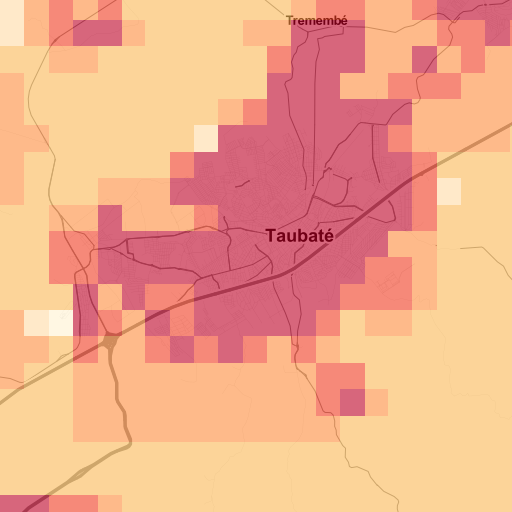
\includegraphics[scale=1]{Figuras/sedacGPWv4.png}
	\caption{\emph{GPWv4: Population Density - 2015} com foco na cidade de Taubaté }
	\label{fig:sedacGPWv4}
\end{figure}

O método de efetuar uma previsão espacial de alta resolução deve considerar como entrada diversos fatores \cite{willis2002spatial}, requer uma grande quantidade de dados, e neste caso, leva em consideração o crescimento local através da obtenção de características regionais usando matrizes de convolução e fatores de ponderação para se obter o crescimento de cada pequena região (quadrícula) de modo que não se ignore nenhuma região e também que tais regiões não ignoradas não venham a causar erros na previsão das demais regiões. Assim, divide-se o mapa de quadrículas em sub regiões compostas por quadriculas, de modo que a previsão ocorra naquela região independente das demais, evitando assim, que regiões mais distantes prejudiquem o processamento de previsão das demais regiões.

A previsão espacial de carga de cada região é feita através do uso de uma função de previsão que tem como entrada, um mapa base \cite{willis2002spatial} e valores otimizados pelo algoritmo competitivo imperialista \cite{atashpaz2007imperialist} modificado \cite{roche2011imperialist} e otimizado (com alterações propostas neste artigo), que por sua vez possui uma função semelhante à função de previsão, porém que possui rotinas para buscar quais valores são os ideais a serem usados para previsão de períodos à frente do mapa base.

São construídos diversos mapas da mesma região, durante diversos períodos diferentes, espaçados igualmente no tempo, para que se possa ser feita uma previsão espacial como uma série temporal de mapas de quadrículas. Algoritmos evolutivos já vem sendo usados para calcular parâmetros de entrada para funções de previsão de séries temporais \cite{whitehead1996cooperative}. No caso de \citeauthor{whitehead1996cooperative}, é criado um algoritmo genético (GA) \cite{mitchell1998introduction} cooperativo-competitivo capaz de evoluir os centros e larguras de uma rede neural RBF \cite{ren2006rbfnn} para ser aplicado na previsão de uma série temporal. Neste trabalho portanto, usa-se o algoritmo competitivo imperialista (ICA) para evoluir valores de uma função proposta capaz de fazer uma "regressão", usando fatores de ponderação e matrizes de convolução para a previsão de crescimento densidade espacial em mapas bidimensionais.

Em resumo, apresenta-se uma técnica capaz de fazer previsão espacial de densidades, sejam elas de quaisquer tipo (carga, populacional, etc.), em alta resolução, que considera diversos fatores na construção dos mapas de quadrículas e que ainda não deixa de ignorar nenhuma área mais afastada da região central urbana, podendo assim melhorar inferência dos resultados obtidos dos métodos de previsão espacial de baseados em quadrículas. 

\section{Objetivos}

O objetivo deste trabalho é efetuar a previsão de densidade espacial genérica (qualquer que seja o parâmetro analisado, densidade de carga, densidade populacional, etc.) sobre um período curto de tempo (de 6 meses a 5 anos), com capacidade de previsão sobre dados dispostos em alta resolução.

Para isto, desenvolve-se uma metodologia capaz de traduzir um conjunto de dados para um histórico de mapas de uma localização que então serão processados por um algoritmo evolutivo, que irá gerar indivíduos capazes de gerar previsões de 1 ou mais períodos a frente com vantagem sobre os modelos estatísticos convencionais. 

Mais especificamente, este trabalho aborda os seguintes tópicos:
\begin{itemize}
\item Modelagem e normalização dos dados para utilização dentro da aplicação.
\item Transformação dos dados iniciais em mapas da mesma localização, durante diferentes períodos, de acordo com o foco da previsão.
\item Regionalização dos mapas para previsão.
\item Definição de uma função de avaliação capaz de fazer previsão espacial sobre regiões.
\item Aplicação do processo evolutivo para definir a melhor curva de crescimento para cada pequena área de uma região.
\item Utilização do resultado do processamento evolutivo para criar as previsões desejadas.
\item Analisar as diferenças entre as previsões geradas pelo modelo proposto com o valores reais e comparar com o modelo de previsão convencional. 
\end{itemize}

\section{Revisão Bibliográfica}
Nesta seção são apresentados, trabalhos que possam servir como base para o desenvolvimento, trabalhos que possuam alguma relação com o objetivo, além de terem suas ideias discutidas para a solução do problema proposto em questão. Alguns conceitos simples e essenciais para o desenvolvimento da metodologia ou experimentos também podem vir a ser abordados.

Um dos conceitos básicos para se iniciar o desenvolvimento de uma metodologia de previsão espacial é a forma com que se definirá o espaço de trabalho e como os dados serão modelados para que o objetivo seja atingido. A proposta deste trabalho é trazer uma metodologia capaz de resultar em uma previsão de espacial sobre áreas urbanas. Assim, é necessário que se utilize dados que traduzam a realidade para os dados a serem processados, convertendo-os e ajustando-os de modo preciso para que não existam erros durante a aquisição e tradução dos dados reais.

Neste caso, este trabalho explora a filosofia de quadrículas, que diz respeito ao particionamento de uma região em pequenas regiões, para a previsão espacial de cargas aplicadas nestas pequenas áreas. Este modelo é apresentado por \citeauthor{willis2002spatial} \cite{willis2002spatial} que enfatizam que o planejamento de sistemas de potência deve sempre incluir a previsão de distribuição de carga, pois tais planos de expansão são baseados em diversas proposições, relacionadas ao crescimento futuro da carga, mesmo que este venha ser definido inadequadamente, seja forçado ou implícito. Assim, ao se utilizar este modelo, consegue-se aumentar a precisão da previsão para atender as necessidades do planejamento. No caso deste trabalho fazemos uma generalização da filosofia para que o modelo possa representar quaisquer tipos de dados, sejam eles do setor elétrico ou qualquer outro.

Atualmente, este método, conhecido também como previsão de pequenas áreas (\emph{small area forecast}) \cite{willis1995spatial}, é amplamente usado para previsão espacial do crescimento do consumo de carga. Não existe um critério fixo para a separação da região em pequenas regiões, porém, a mais comumente utilizada é a separação em regiões não uniformes, tais que cada uma represente uma região correspondente ao mapeamento elétrico da área de distribuição, sendo esta divisão definida por critérios como área de distribuição de subestações, ou áreas de atuação de concessionárias etc.. Outra forma, é a separação em regiões uniformes, quadradas que se encaixam em diversas situações, por manter o toda região homogênea e normalizada, denominada a filosofia de quadrículas ou quadriculamento da região. A Figura \ref{fig:RegionsAndQuadrics} mostra como pode ser dividido um mapa de uma região usando ambos os modelos citados no parágrafo anterior. 

\begin{figure}[h]
	\centering	
	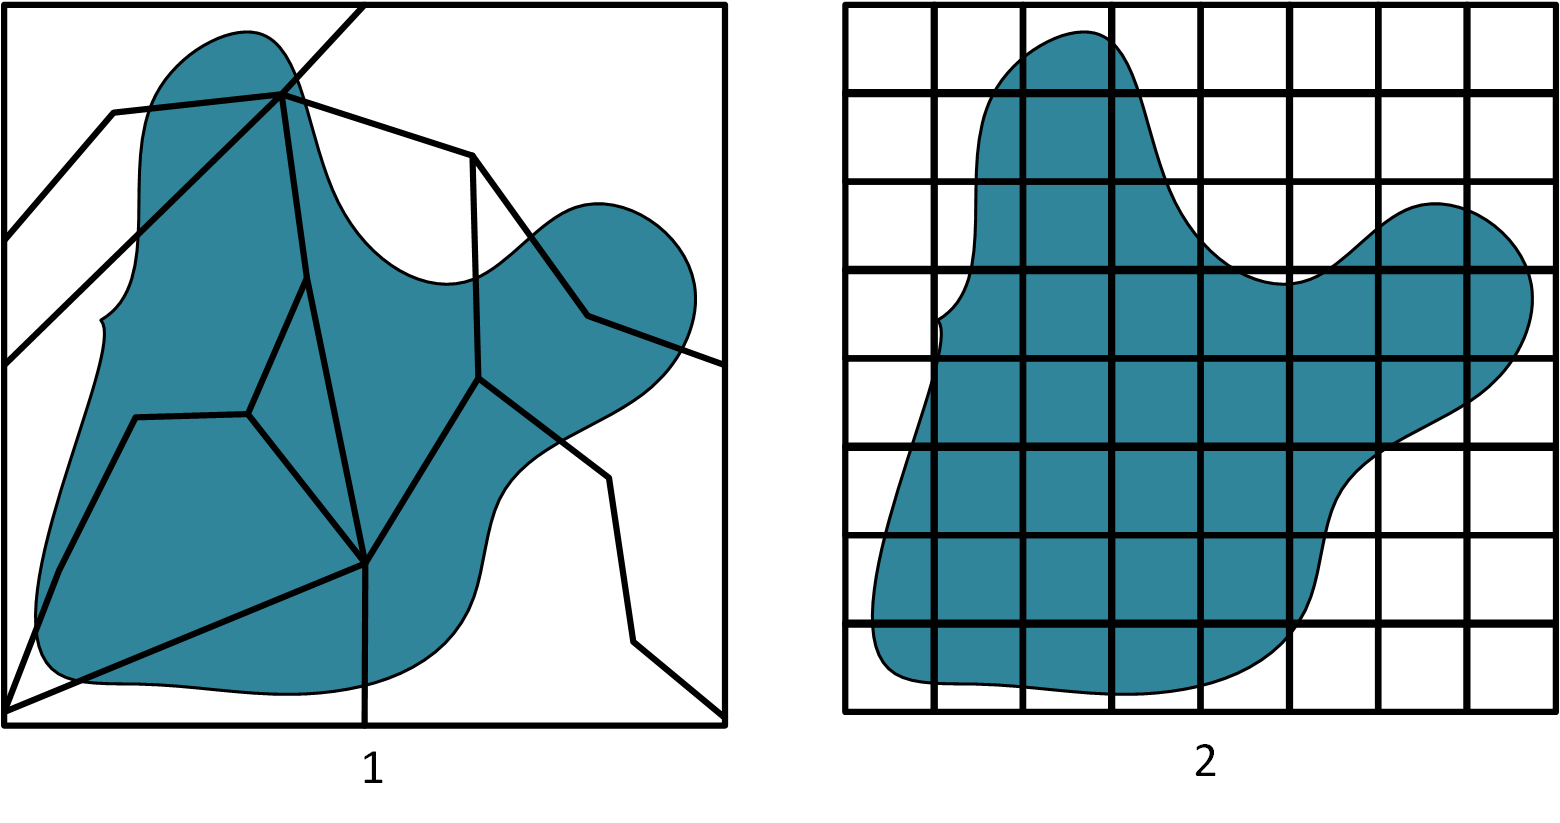
\includegraphics[scale=0.55]{Figuras/RegionsAndQuadrics.png}
	\caption{Regiões e Quadrículas}
	\label{fig:RegionsAndQuadrics}
\end{figure}

Ambas possuem vantagens e desvantagens segundo \citeauthor{willis2002spatial} \cite{willis2002spatial}, como por exemplo, a separação por quadrículas, ilustrada no item 2 da figura, pode produzir melhores resultados, porém pode ser mais complexo obter e processar os dados para formar as regiões. E a separação por regiões apesar de possuir sua separação formada por dados que classificam a região de alguma forma, é mais complexa de ser modelada computacionalmente para análise homogênea, pois suas área são de tamanhos e formas diferentes.

Existem muitos métodos de previsão de pequenas áreas, portanto eles sempre se encaixam em uma das duas categorias (definido por \citeauthor{willis2002spatial} \cite{willis2002spatial} e detalhado por \citeauthor{arango2000thesis} \cite{arango2000thesis}, sendo:

\begin{itemize}
\item Métodos de ajuste, que considera a curva de tendência do crescimento de períodos passados, ajustando-a através de métodos como mínimos quadrados, média móvel, etc. de modo que os períodos futuros possam ser extrapolados a partir desta curva ajustada.
\item Métodos baseados no uso da terra, que faz as previsões futuras baseando-se na análise de fatores de uso da terra, como planos diretores, zoneamentos, entre outros, os quais possam ser retiradas informações de como os crescimentos de carga (de regiões residenciais, industriais ou comerciais) irão crescer durante os períodos futuros.
\end{itemize}

No caso deste trabalho, o método desenvolvido se aplica principalmente ao primeiro modelo de métodos, apesar de processar os dados obtidos de modo que eles sejam transformados em informações de crescimento de carga residencial durante os períodos, ao processar tais dados, leva-se em consideração como estes dados crescem ao longo dos períodos, de modo que se possa gerar uma curva de tendência e extrapolar uma previsão de períodos futuros. O segundo método é usado apenas inicialmente, ao se ajustar os dados para que eles possam ser normalizado e traduzidos para um mapa de quadrículas, porém não se faz nenhum tipo de previsão ou geração de regras de previsão durante esta etapa de tradução.

Um modelo dinâmico de expansão de cargas é proposto por \citeauthor{arango2000thesis}, e baseia-se em conceitos de análise locacional, que aplica a teoria dos polos urbanos e se encaixa mais nos métodos baseados no uso da terra (segundo item). Deste modo, ele cria um simulador de expansão de cargas que evolui de forma dinâmica e continua as condições para uma nova unidade de carga. Tal modelo consegue representar a expansão de carga, usando uma adaptação do processo de recozimento simulado que fora especificamente desenvolvido para solucionar o problema. Este trabalho traz uma solução mais genérica, para a previsão de expansão de densidades, seja ela de cargas, populacional, entre outras.

Uma análise interessante sobre o erro de previsão espacial é desenvolvida por \citeauthor{arango2000thesis}, que avalia o erro de previsão espacial considerando as diferenças entre os valores reais e estimados para cada subárea urbana, e traz um exemplo muito bom, que demonstra a preocupação para com a avaliação da imprecisão dos modelos de previsão espacial. No exemplo ele imagina duas regiões, as quais tenham uma magnitude total de cargas iguais, porém distribuídas diferentemente, como mostra a Figura \ref{fig:ErrorDistArango}.

\begin{figure}[h]
	\centering	
	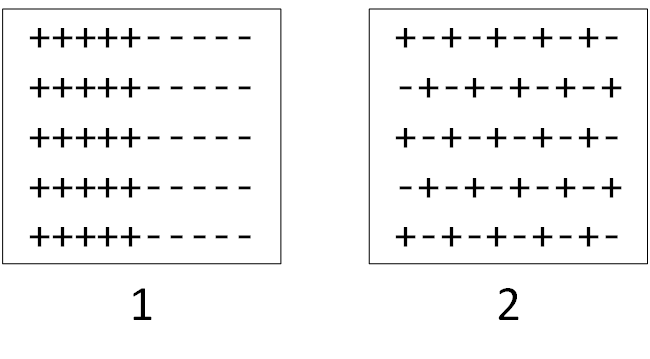
\includegraphics[scale=2]{Figuras/Ilustration-ErrorDistArango.png}
	\caption{Distribuições distintas do mesmo erro global, detalhado em \cite{arango2000thesis} e definido por \cite{willis1995spatial}}
	\label{fig:ErrorDistArango}
\end{figure}

A estimativa para ambas as áreas serão completamente distintas, sendo que na primeira existe uma tendencia bem direcionada e na segunda ocorrerá uma estimativa muito mais homogênea em relação a região. 

Ao se fazer uma análise estatística entre a uma região estimada e sua região real, comparando o erro absoluto de cada pequena área (quadrícula). É possível ocorrer que uma região seja estimada de forma absolutamente correta, assim como também pode ocorrer que uma região seja estimada de forma totalmente incorreta. Neste trabalho trabalha-se para que tais erros sejam minimizados de modo a fazer com que toda região tenha uma estimativa com o menor erro possível, seguindo as taxas de crescimento tanto das pequenas áreas, quanto da região como um todo, e ainda, também agrega o crescimento das pequenas áreas presentes nas redondezas da pequena área que esteja sendo analisada.

Para o desenvolvimento da aplicação foi necessária inicialmente a modelagem dos dados iniciais de modo que estes fossem convertidos com a menor ou nenhuma quantidade de erro residual. Pois neste caso, os dados estão representados em coordenadas geográficas, e são utilizadas diversos cálculos de distância para que eles sejam adequadamente identificados em sua pequena região. Para se calcular a distância entre dois pontos, dispostos em um mapa terrestre em coordenadas cartesianas, pode-se aplicar o teorema de Pitágoras:

\[d = \sqrt{(X2 - X1)^2 + (Y2 - Y1)^2}\]

Sendo \((X1, X2)\) e \((Y1,Y2)\) os pontos iniciais e finais de longitude e latitude respectivamente.

Esta fórmula de cálculo de distância, quando aplicada a pontos cuja distância é menor que 20 km, produz erros dependentes de suas posições reais dispostas no globo, sendo que tais erros variam como:
\begin{itemize}
\item De 0 a 30 metros para latitudes menores que 70 graus.
\item De 0 a 20 metros para latitudes menores que 50 graus. 
\item De 0 a 9 metros para latitudes menores que 30 graus.
\end{itemize}

Tal gestão de erros é desnecessária quando se usa a distância calculada pela fórmula de Haversine \cite{shumaker1984astronomical}, que calcula a distância entre dois pontos dispostos na superfície de uma esfera, relacionando os lados aos ângulos de uma esfera triangular. Assim, fazendo o uso de um mapa terrestre esférico, onde tal esfera possui raio \(R\), e tendo a representação dos pontos que se deseja calcular a distância como vetores compostos na forma (Longitude, Latitude), temos que o \(ponto1 = (lon1,lat1)\) e o \(ponto2 = (lon2,lat2)\), calculamos a distância como mostra a expressão:

\[dlon = lon2 - lon1\]
\[dlat = lat2 - lat1\]
\[a = \sin^2\left(\frac{dlat}{2}\right) + \cos(lat1) \cdot \cos(lat2) \cdot \sin^2\left(\frac{dlon}{2}\right)\]
\[c = 2 \cdot \arcsin(\min(1,\sqrt{a}))\]
\[d = R \cdot c\]

A distância calculada resulta em um valor exato, tanto computacionalmente quanto matematicamente, onde \(c\) é a distância do caminho mais curto entre os dois pontos, denominada ortodromia, representada em radianos, que multiplica \(R\), convertendo o resultado de d para a mesma unidade do Raio \(R\). 

A função \(min\) protege contra possíveis erros de arredondamento que podem sabotar a computação do arco-seno caso os dois pontos estejam em lados opostos da terra. Sob estas condições, a Fórmula Haversine é mal condicionada, mas o erro, que talvez pareça grande, que chega a ser de aproximadamente 2 km, está no contexto de uma distância próxima 20,000 km, sendo que este erro é de aproximadamente 0.00001\% da distância total.

No ambiente computacional, a maioria das funções ou componentes trigonométricos são expressados em radianos. Uma vez que os dados de coordenadas (Longitude e Latitude) geralmente estão expressos na forma Graus, Minutos e Segundos, é necessário convertê-los para graus decimais:

\[
\begin{matrix}
coordDec = 
& coordGMS.Graus +\\ 
& \left(\frac{CoordGMS.Minutos}{60}\right) +\\ 
& \left(\frac{CoordGMS.Segundos}{3600}\right)
\end{matrix}
\]

Com as coordenadas convertidas para graus decimais, ainda é necessário convertê-las para radianos, que é simplesmente multiplicar a coordenada em graus decimais por \(\frac{\pi}{180}\):

\[coordRad = \frac{coordDec \cdot \pi}{180}\]

Por fim, a definição de \(R\) como sendo o raio da esfera, deve ser levado em consideração que o planeta Terra não é uma esfera perfeita, mas sim, possui uma forma chamada esferóide oblato (Figura \ref{fig:OblateSpheroid}), e portanto, deve-se considerar diferentes raios para diferentes posições de latitude, uma vez que o achatamento ocorre nos polos.  

\begin{figure}[h]
	\centering	
	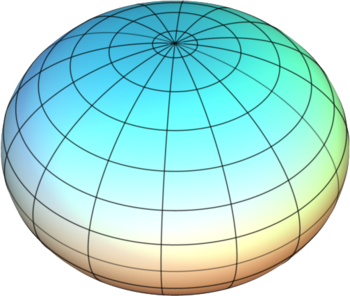
\includegraphics[scale=0.3]{Figuras/OblateSpheroid.PNG}
	\caption{Esferóide oblato}
	\label{fig:OblateSpheroid}
\end{figure}

A circunferência oficial terrestre é de 40003.2 km, que provém da definição de uma milha náutica, que historicamente é definida como 1 arco de minuto medido, à superfície média do mar, ao longo de um qualquer grande círculo da Terra. Como a terra não é uma esfera, tal definição é ambígua. Então, o valor aceito internacionalmente(SI) para uma milha náutica é de exatamente 1.852 km. Deste modo, define-se como circunferência terrestre, o valor de 40003.2 km:

\[40003.2 (km) = 360(grau) * 60\left(\frac{minuto}{grau}\right) * 1.852\left(\frac{km}{minuto}\right)  \]

Implicando então que o raio \(R\) seja de:

\[R = \frac{40003.2}{(2 \cdot \pi)} = 6367 (km) \]

Como o planeta Terra não é representado por uma esfera, mas sim por um esferóide oblato, e possui um Raio Polar de 6357 km e um raio equatorial de 6378 km, uma aproximação satisfatória seria como mostra a expressão:

\[R = 6378 - 21 \cdot \sin(lat) \]

Porém, tal aproximação é dependente apenas do valor de latitude, e o raio da curvatura é dependente não só do valor de latitude, mas também da direção, de acordo com \cite{snyder1987map}. Então, usa-se:

\[R = \frac{ a \cdot (1 - e^2)}{ (1 - e^2 \cdot \sin^2(lat))^\frac{3}{2}}\]

Onde \(a\) é o raio equatorial, \(b\) o raio polar, e \(e\) é a excentricidade do 
\(\text{elipsóide} = \left(1 - \frac{b^2}{a^2}\right)^\frac{1}{2}\). 
Então tem-se que \(e = 0.0167086\). Assim, haverá um erro mínimo sempre que as distâncias entre dois pontos de coordenadas geográficas forem calculadas utilizando a fórmula de haversine.

Este trabalho utiliza-se muito da fórmula de haversine para converter os dados iniciais, dispostos em coordenadas geográficas, para coordenadas cartesianas, de modo que se crie uma matriz de pequenas áreas (quadrículas), onde estas pequenas áreas possam vir a ser usadas para gerar um mapa cartesiano que represente fielmente os dados que foram convertidos, tanto para o processamento destes dados quanto para a apresentação dos resultados.

A previsão espacial apresentada por este trabalho é efetuada usando-se um algoritmo que classifica-se como evolutivo, isto é, está na mesma categoria que algoritmos como algoritmos genéticos (AG) \cite{mitchell1998introduction} e otimização por enxame de partículas (PSO). \cite{atashpaz2007imperialist} apresenta o algoritmo imperialista competitivo (ICA), que atinge resultados tão bem quanto algoritmos genéticos, atingindo o mínimo global geralmente ao mesmo tempo que o algoritmo genético. 

A vantagem do ICA sobre o GA se dá em relação média do custo de toda população, onde o GA geralmente fica estagnado em um patamar devido ao fato de que sempre que ocorrem mutações, seleções ou criação de novos indivíduos para complementar a população, estes indivíduos são gerados com valores aleatórios, impossibilitando a convergência de toda a população para a solução ótima. O ICA por sua vez consegue fazer com que toda a população seja convergida para a solução ótima, sem que fique estagnado ou ceia em mínimos locais.  

Outra sutil vantagem que o ICA possui sobre o GA é o fato de seus atributos serem valores numéricos de ponto flutuante, uma vez que no GA em sua versão canônica, utilizam-se vetores de atributos binários, que, desta forma, seria sempre necessário traduzir o valor do cromossomo para valores numéricos. 

Este trabalho utiliza um grande conjunto de números de ponto flutuante para sua função de avaliação, que são traduzidos para estruturas usadas pela função. Caso o vetor de atributos fosse de valores binários, seriam necessária uma tradução dos valores binários para valores numéricos de ponto flutuante, antes mesmo de se gerar as estruturas usadas pela função de avaliação, tornando este processo muito mais complexo.

\cite{roche2011imperialist} traz uma aplicação concreta do ICA voltado para otimizar o uso de ferramentas que definem estrategicamente a alocação de unidades de geração de energia para as usinas de acordo com diversos parâmetros. O ICA é comparado com modelos convencionais, como AG e PSO, tendo uma efetividade maior tanto em previsão quanto em velocidade. Voltando o Foco para a o desenvolvimento do ICA feito por \citeauthor{roche2011imperialist}, ele desenvolveu o ICA na linguagem Java, que pode ser acessado pelo repositório git em github.com/robinroche/jica \cite{jica}, sendo desenvolvido em uma linguagem orientada a objetos, de forma simples. Este trabalho propõe uma melhora na implementação orientada a objetos para o ICA de modo que ele possa ser usado genericamente para qualquer caso ou aplicação, de modo que a modelagem de qualquer problema seja rápida, prática, modular e sem a necessidade de alterar o código fonte principal da lógica do ICA. 

Tendo conhecimento que o desenvolvimento de uma metodologia para previsão espacial apresenta uma solução de alta complexidade, exige elevada quantidade de informação e a qual se deve levar em conta diversos fatores de crescimentos aleatórios e/ou imprevisíveis (como desejo político ou planejamento externo), tais problemas apresentam soluções de domínio não lineares. Assim, este trabalho propõe uma implementação diferenciada do ICA de forma que este seja capaz de atender a todas as requisições do problema de forma prática, precisa e rápida. 

A metodologia empregada faz uso do ICA para previsão espacial, em um ambiente (neste caso, urbano) bidimensional (2D). Então, para que tal problema possa ser solucionado de modo que múltiplas alterações sejam executadas e testadas afim de se obter os melhores resultados, algumas adaptações foram imprescindíveis ao ICA tanto em relação a otimização de seu desempenho na busca de soluções melhores em um tempo menor  quanto a organização e modelagem do conceito, que se deu na forma de uma implementação orientada a objetos \cite{booch1982object} e \cite{coad1991object}. 

A primeira preocupação durante o desenvolvimento foi encontrar quais seriam as abordagens mais certeiras e inovadoras para que a previsão de densidade espacial urbana fornecesse resultados aceitáveis. Tendo isto em mente, sabia-se que deveriam ocorrer diversos testes com diversas funções de avaliação diferentes, e ainda, que tais funções, devido a complexidade do problema, também teriam de ser diversas vezes ajustadas durante os testes. Assim, a aplicação dos conceitos de orientação a objetos foram utilizados para a modelagem do ambiente, para a implementação dos conceitos do ICA e de diversas funções de avaliação ou modelos de problemas diferentes.





\section{Estrutura da Dissertação}


Este documento está dividido nos capítulos: Introdução, Metodologia, Desenvolvimento, Experimentos e Resultados e Conclusão.

No capítulo introdução é contextualizado o conceito de previsão espacial urbana, que pode ser feita a partir de diversos métodos e técnicas. Também são apresentados os objetivos definidos e a justificativa da realização do trabalho.

Em Metodologia são detalhados os principais conceitos e técnicas pesquisados e aplicados no trabalho, abrangendo principalmente o Algoritmo Imperialista Competitivo e a operação matemática de convolução.

O capítulo Desenvolvimento descreve especificamente como as técnicas escolhidas foram desenvolvidas, modificadas e implementadas focando nos objetivos e na solução do problema.

Já no capítulo Experimentos e Resultados são apresentados como o ambiente foi modelado, como o método proposto se comportou sobre uma e sobre muitas regiões, e apresentação dos resultados sobre dados reais, apresentando os resultados em forma de imagens de alta resolução e uma tabela comparativa.

Por fim, no capítulo Conclusão são considerados os resultados obtidos frente aos objetivos propostos, a colaboração deste trabalho, assim como a indicação de trabalhos futuros para a continuidade da pesquisa.




\chapter{Metodologia}
\label{Metodologia}
%\externaldocument[met-]{metodologia}


Neste capítulo são apresentados os conceitos do algoritmo imperialista competitivo, a apresentação da operação de convolução e a convolução de imagens e a apresentação do Previsor Espacial de Mapas de Densidade, seguidos de uma breve análise sobre estes assuntos, direcionando como estes conceitos serão aplicados na busca da solução para o problema proposto.

\section{Algoritmo Imperialista Competitivo}

O algoritmo imperialista competitivo \cite{atashpaz2007imperialist} (ou ICA - \emph{Imperialist Competitive Algorithm} em inglês) é um algoritmo de busca, caracterizado como evolutivo, e baseado na ideia da disputa entre impérios pela extensão de seus domínios para além de seus territórios, aplicável à topologias complexas e com soluções não triviais. Para que um império aumente seu poder ele deve aplicar sua influência sob mais territórios dominando-os e assimilando-os. Territórios dominados por países imperialistas são chamados de colônias, e um império é denominado pelo conjunto formado por um país imperialista e suas colônias.

As colônias de um império tendem a ter suas características se assemelhando às de seu país imperialista a cada década que passa. Esta tendência pode ser vista como uma forma de movimento, ou seja, uma colônia se move em direção ao seu país imperialista de forma que suas características se pareçam mais com as dele.

A definição do poder dos países, sejam eles imperialistas ou colônias, é baseado na ideia de que um dado país tem um custo para se manter. Se um país é rico em recursos, significa que ele terá um custo muito baixo, e consequentemente poderá usar seus recursos de forma a expandir suas fronteiras através da assimilação de colônias. Assim o poder de um país é definido pelo inverso de seu custo, implicando em quando um país possuir um custo muito próximo de (ou tender a) zero, isto significará que seu poder seria imenso e tenderia a infinito.

Antes que a disputa imperialista comece, todos os países são gerados com características aleatórias. Os custos dos países gerados são calculados, e consequentemente seus poderes são definidos. Uma porcentagem dos países com maior poder se tornam impérios, e o restante se tornam colônias. As colônias são distribuídas aos impérios mais poderosos de uma forma proporcional.

Impérios disputam entre si usando como forma de medição o nível de poder total, que por sua vez é definido pela soma do poder do país imperialista com o poder de suas colônias. Assim, países imperialistas mais fortes tendem a tomar as colônias de um imperialista mais fraco, e os imperialistas mais fracos tendem a perder suas colônias para imperialistas mais fortes até que eles não tenham mais nenhuma colônia e sejam eliminados da disputa. 

Uma colônia pode se tornar um país imperialista quando seu poder superar o poder de seu atual imperialista, assim, todas as colônias do país imperialista, incluindo ele mesmo, passam a ser colônias da colônia que se tornou o novo país imperialista, alterando assim, a direção do movimento das colônias para a posição deste novo imperialista.

O resultado deste processo competitivo tende para que reste apenas um império na disputa possuindo todas as colônias, de forma que todas as colônias tenham as mesmas características se igualando às seu país imperialista.

Sendo o ICA um algoritmo de busca, seu objetivo é encontrar uma solução dentre diversas outras, tal que esta seja ótima, em termos das variáveis do problema (dimensões) em questão.  Como pode ser visto na Figura \ref{fig:Fluxograms-ICACanonic} antes de começar o processo evolutivo, deve-se inicializar os países formando os impérios e as suas respectivas colônias. Sendo assim, inicialmente deve-se definir a estrutura básica de um país que, analogamente a um cromossomo presente no algoritmo genético canônico (GA - \emph{Genetic Algorithm}), usa um vetor de valores de dimensão \(1xN_{var}\) apresentado pela equação \ref{eq:ica1}:

\begin{equation}
\label{eq:ica1}
\text{país} = [p_{1},p_{2},...,p_{N_{var}}] 
\end{equation}

Sendo que os elementos contidos no vetor representem as características deste país com valores numéricos de ponto flutuante, diferentemente do GA canônico, que usa uma tripa de valores booleanos que geralmente devem ser traduzidos quando se deseja usar valores numéricos. E define-se \(N_{var}\) o número de dimensões do problema a ser otimizado. 

\begin{figure}[h]
	\centering	
	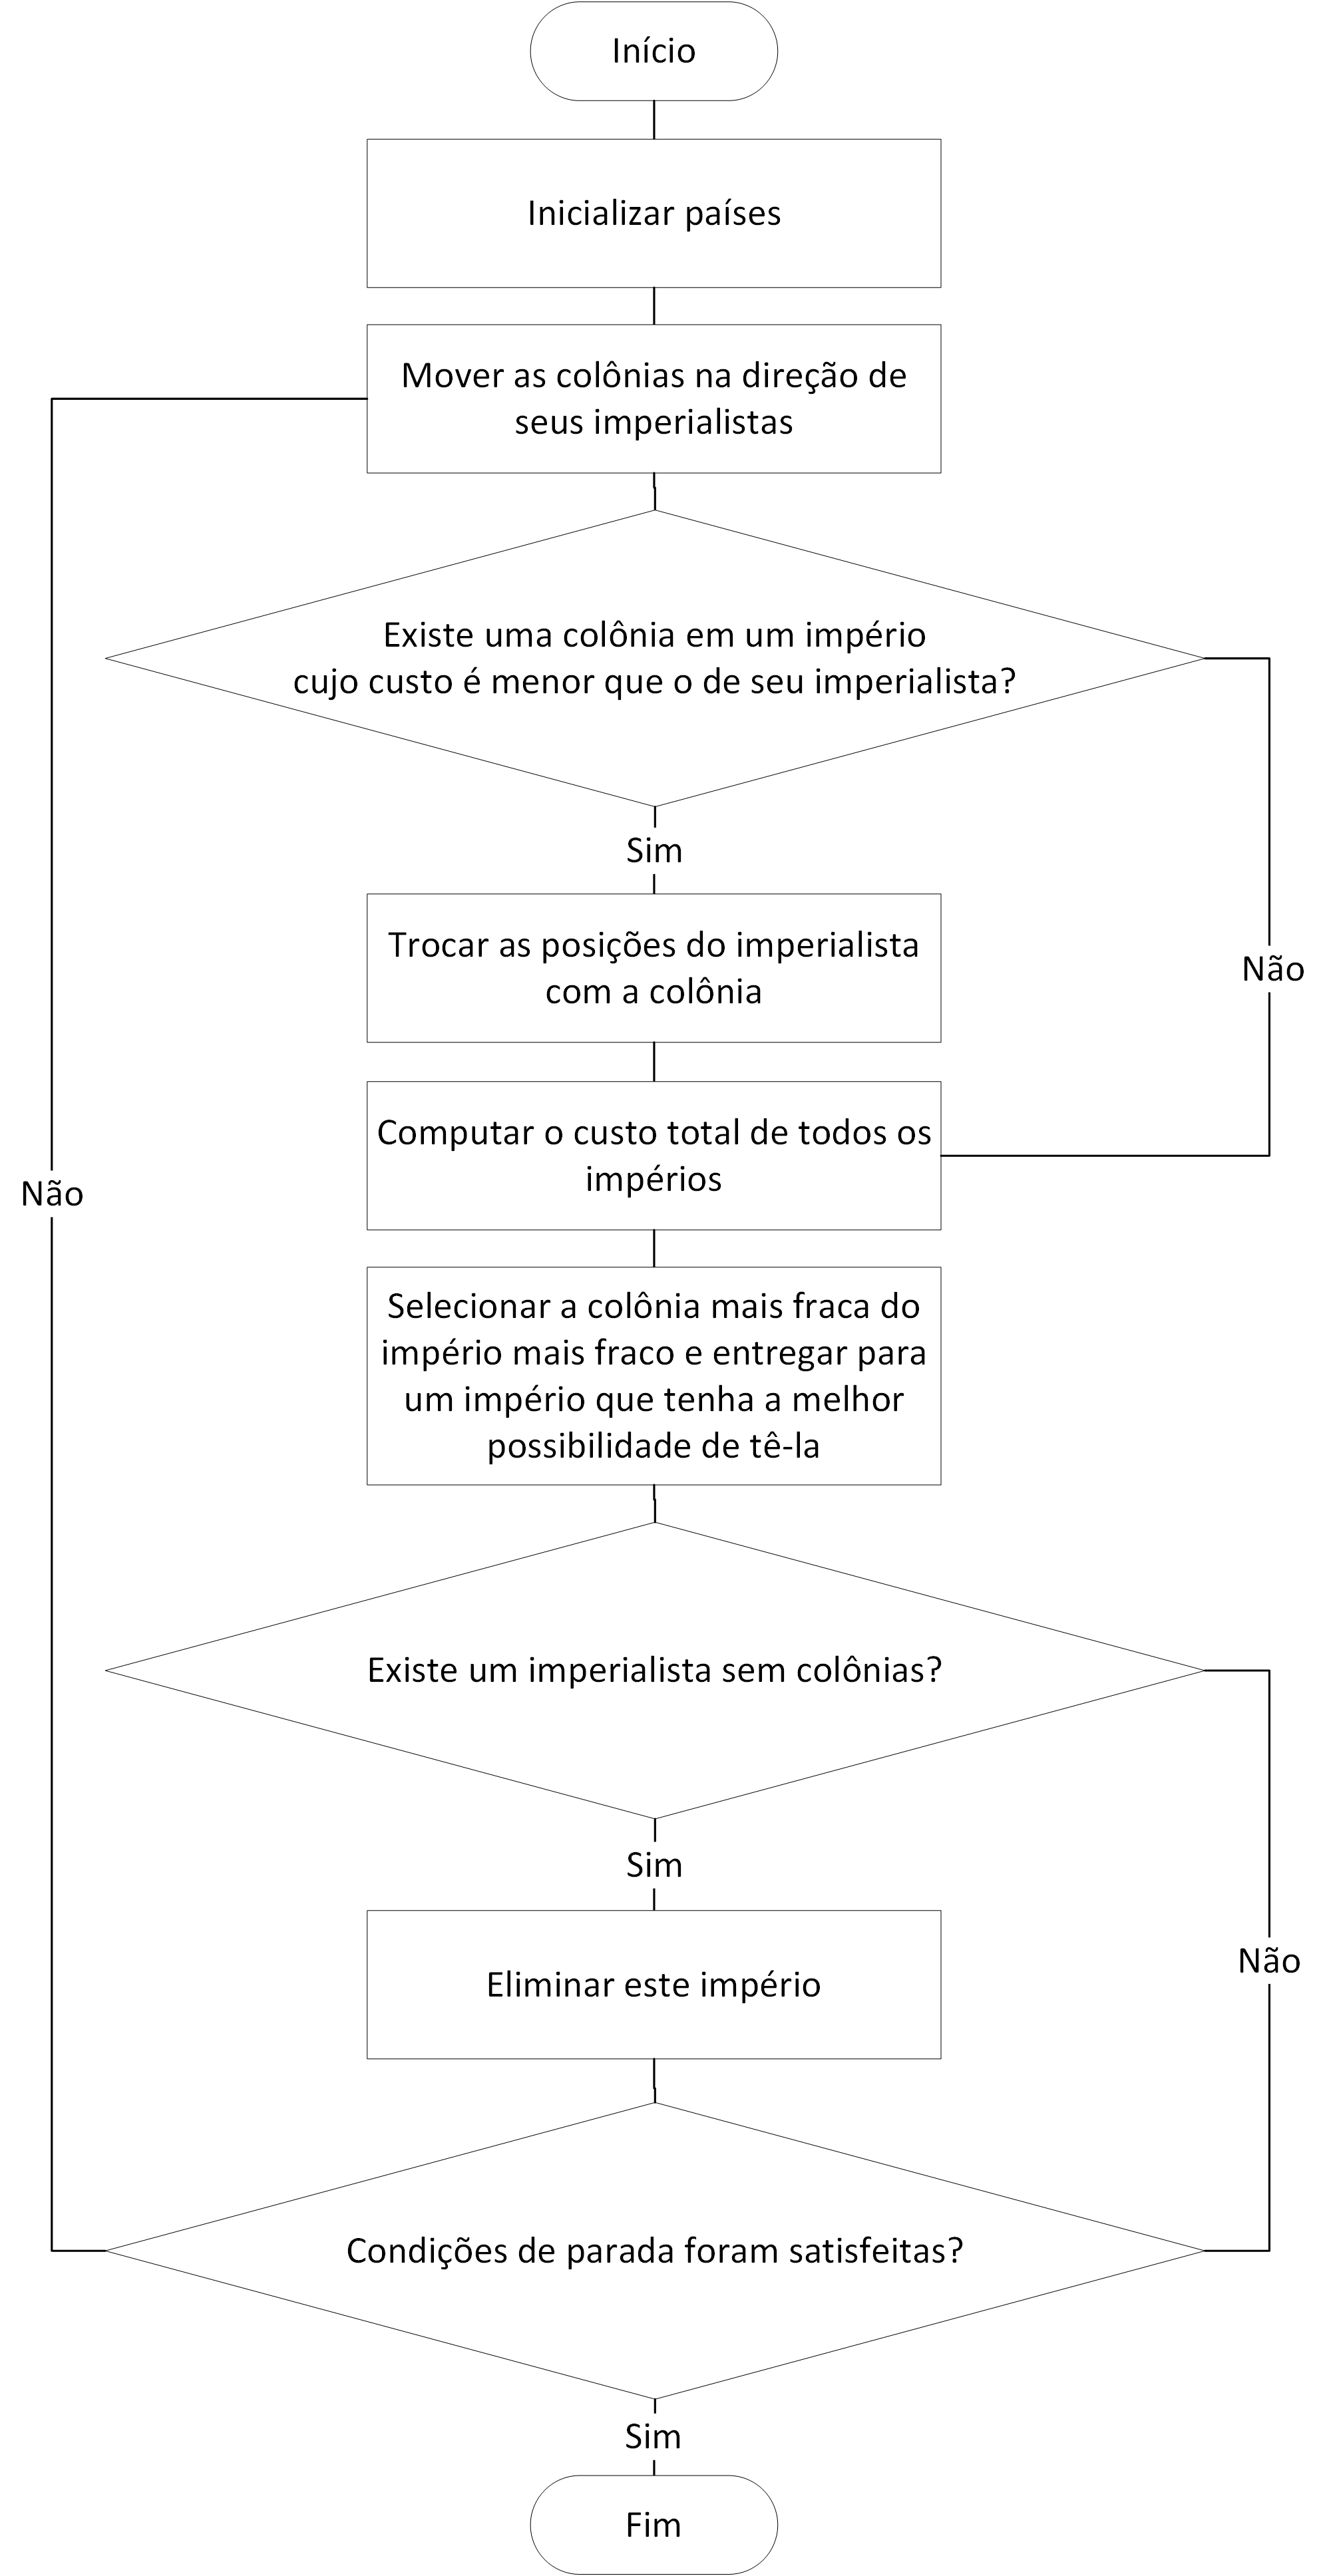
\includegraphics[scale=0.55]{Figuras/Fluxograms-ICACanonic.png}
	\caption{Fluxograma ICA canônico}
	\label{fig:Fluxograms-ICACanonic}
	\end{figure}

O custo de um país deve ser calculado através da aplicação dos valores presentes no país a uma função \(f\) de acordo com a equação \ref{eq:ica2}:

\begin{equation}
\label{eq:ica2}
custo = f (\text{país}) = f (p_{1},p_{2},...p_{N_{var}})
\end{equation}

Sendo o custo um valor análogo ao valor de aptidão de um cromossomo no algoritmo genético e \(f\) uma função de avaliação.

Um valor inicial \(N_{pop}\) define a quantidade de países que serão gerados com valores (características) aleatórios na sua inicialização, antes que se comece a etapa de otimização (competição imperialista). Seleciona-se também uma porção de \(N_{pop}\), denominada \(N_{imp}\), como sendo o número de países imperialistas inicial. A partir disso, são escolhidos como os \(N_{imp}\) países imperialistas, os países mais poderosos dentre os \(N_{pop}\) países. A quantidade de países restantes é denominada \(N_{col}\), tal como mostra a equação \ref{eq:ica3}: 

\begin{equation}
\label{eq:ica3}
N_{col} = N_{pop} - N_{imp} 
\end{equation}

E que posteriormente serão distribuídas proporcionalmente a cada um dos imperialistas.

Para a distribuição  das \(N_{col}\) colônias para os \(N_{imp} \) imperialistas ser feita de modo proporcional ao poder de cada um destes países imperialistas, define-se o valor normalizado do custo de um imperialista segundo a equação \ref{eq:ica4}

\begin{equation}
\label{eq:ica4}
C_{n} =  c_{n} - maxi{c_{i}}
\end{equation}

Onde \(C_{n}\) é o custo atual do n-ésimo imperialista, \(c_{n}\) é o custo normalizado deste enésimo imperialista, e a operação \(maxi{c_{i}}\) representa o valor máximo dos custos dentre todos os países. Assim, pode-se definir o poder normalizado de cada país imperialista como mostra a equação \ref{eq:ica5}:

\begin{equation}
\label{eq:ica5}
P_{n} = \left| \frac{C_{n}}{\sum_{i=1}^{Nimp}C_{i}}\right| 
\end{equation}

Que é basicamente o custo normalizado do enésimo imperialista dividido pela soma dos custos normalizados dentre todos os imperialistas. Sendo assim, este poder normalizado pode ser entendido como um valor que representa a porção de colônias que devem ser possuídas por aquele imperialista. Então o número de colônias de um império é definido pela equação \ref{eq:ica6}:

\begin{equation}
\label{eq:ica6}
N.C.n = arredondamento ( P_{n} \cdot N_{col})
\end{equation}

Sendo \(N.C.n\) o número inicial de colônias do enésimo imperialista.

Com os impérios já formados, contendo um país imperialista e suas colônias, a sequencia do fluxograma indica que as colônias de um império devem se movimentar em direção ao seu país imperialista, como pode ser visto na Figura \ref{fig:Ilustrations-ColonyEmpireMove}. O movimento de uma colônia até seu imperialista deve ser calculado considerando um fator aleatório e um fator de controle de intensidade, sendo que o fator aleatório pode ser de distribuição uniforme (ou qualquer outra que seja apropriada a situação) e  o fator de controle de intensidade deve ser relativo ao império, portanto usa-se a distância entre o imperialista e a colônia. Assim, tem-se que um valor \(x\), representado o movimento que será efetuado pela colônia, seja o produto vetorial entre a distância e o fator aleatório, como mostrado na equação \ref{eq:ica7} a seguir:

\begin{equation}
\label{eq:ica7}
x  = URand(0, \beta \times d)
\end{equation}

Sendo \(\beta\) um valor aleatório maior que 1 e \(d\) a distância absoluta entre o país imperialista e a colônia.

\begin{figure}[h]
	\centering	
	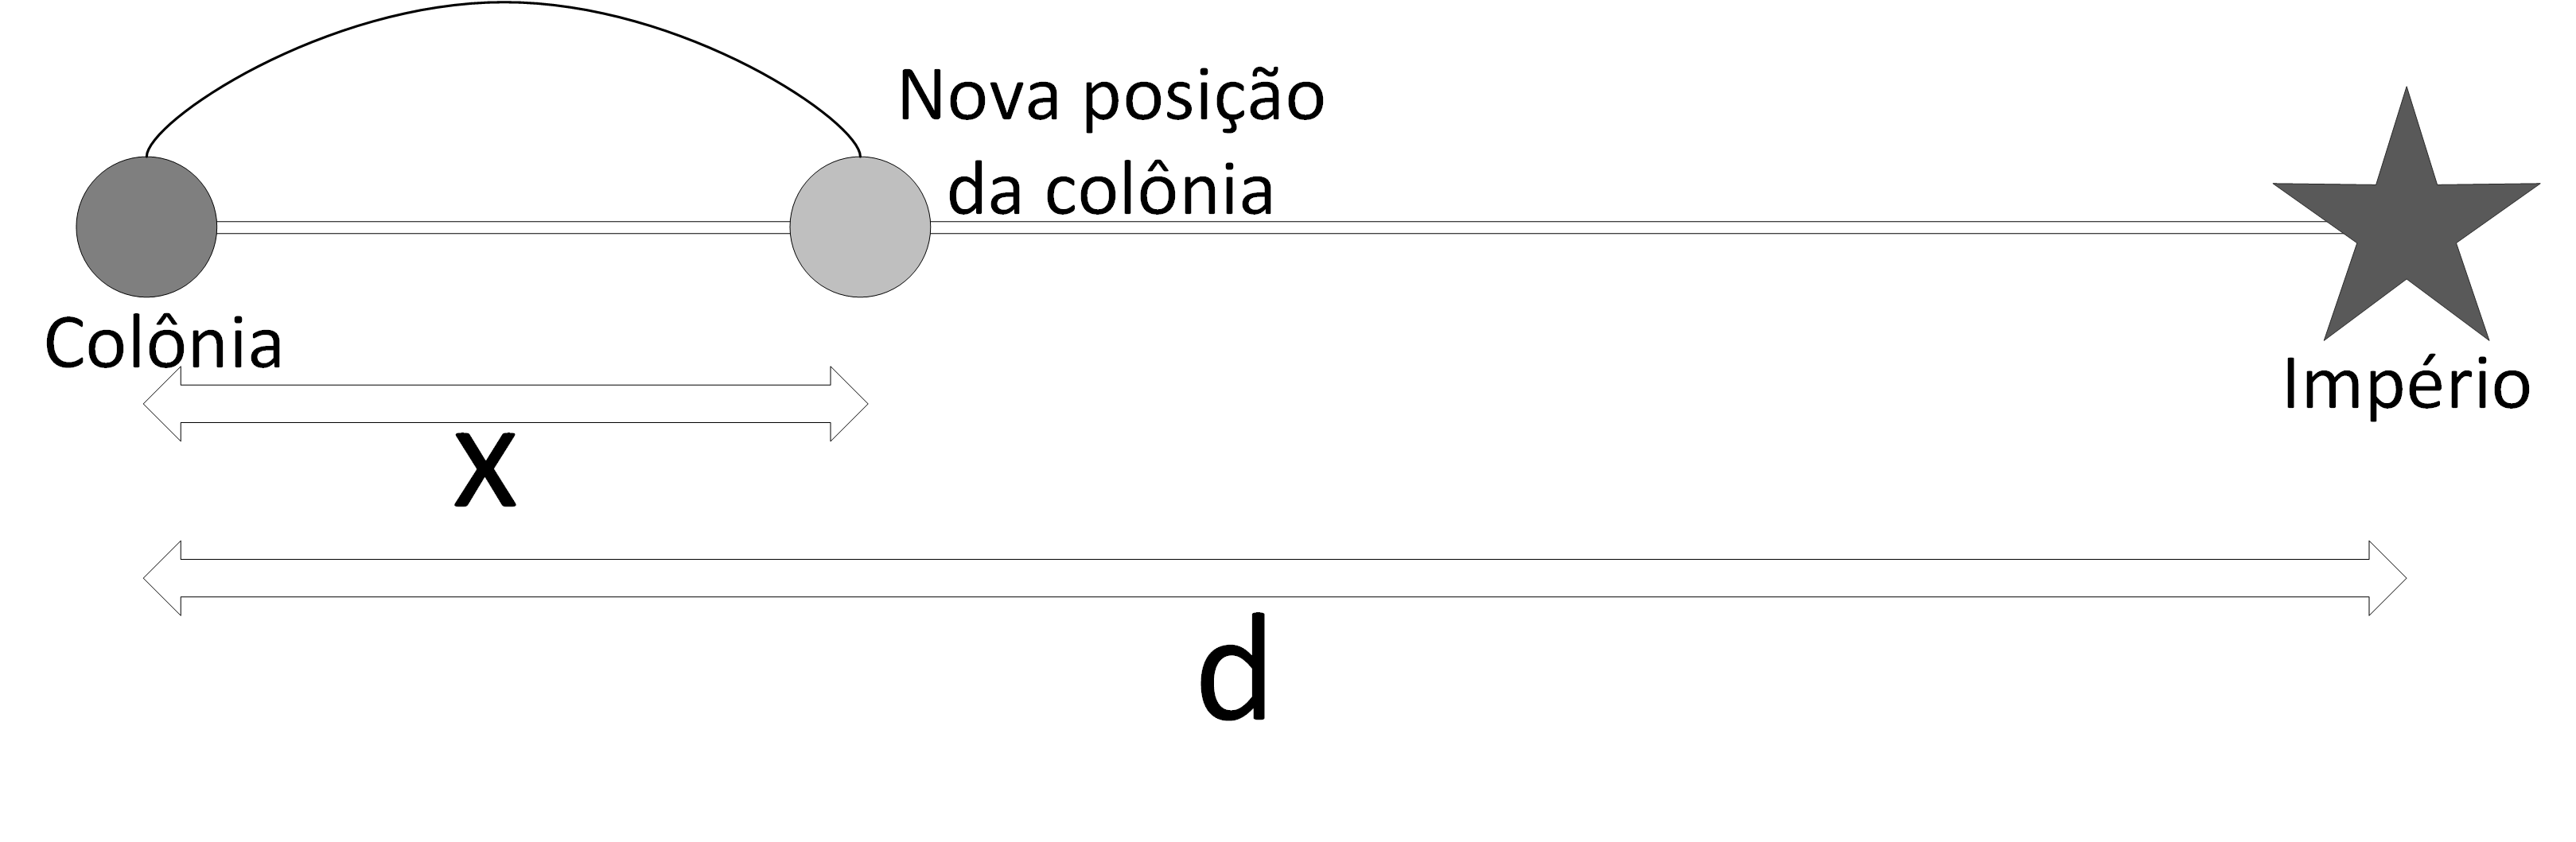
\includegraphics[scale=0.5]{Figuras/Ilustrations-ColonyEmpireMove.png}
	\caption{Movimento da colônia para seu imperialista}
	\label{fig:Ilustrations-ColonyEmpireMove}
\end{figure}

Usa-se \(\beta\) maior que 1 por resultar em um efeito elástico no espaço de busca, fazendo que uma colônia se aproxime de seu imperialista explorando ambos os lados da dimensão como pode ser visto na Figura \ref{fig:Ilustrations-BetaComparison}. 

\begin{figure}[h]
	\centering	
	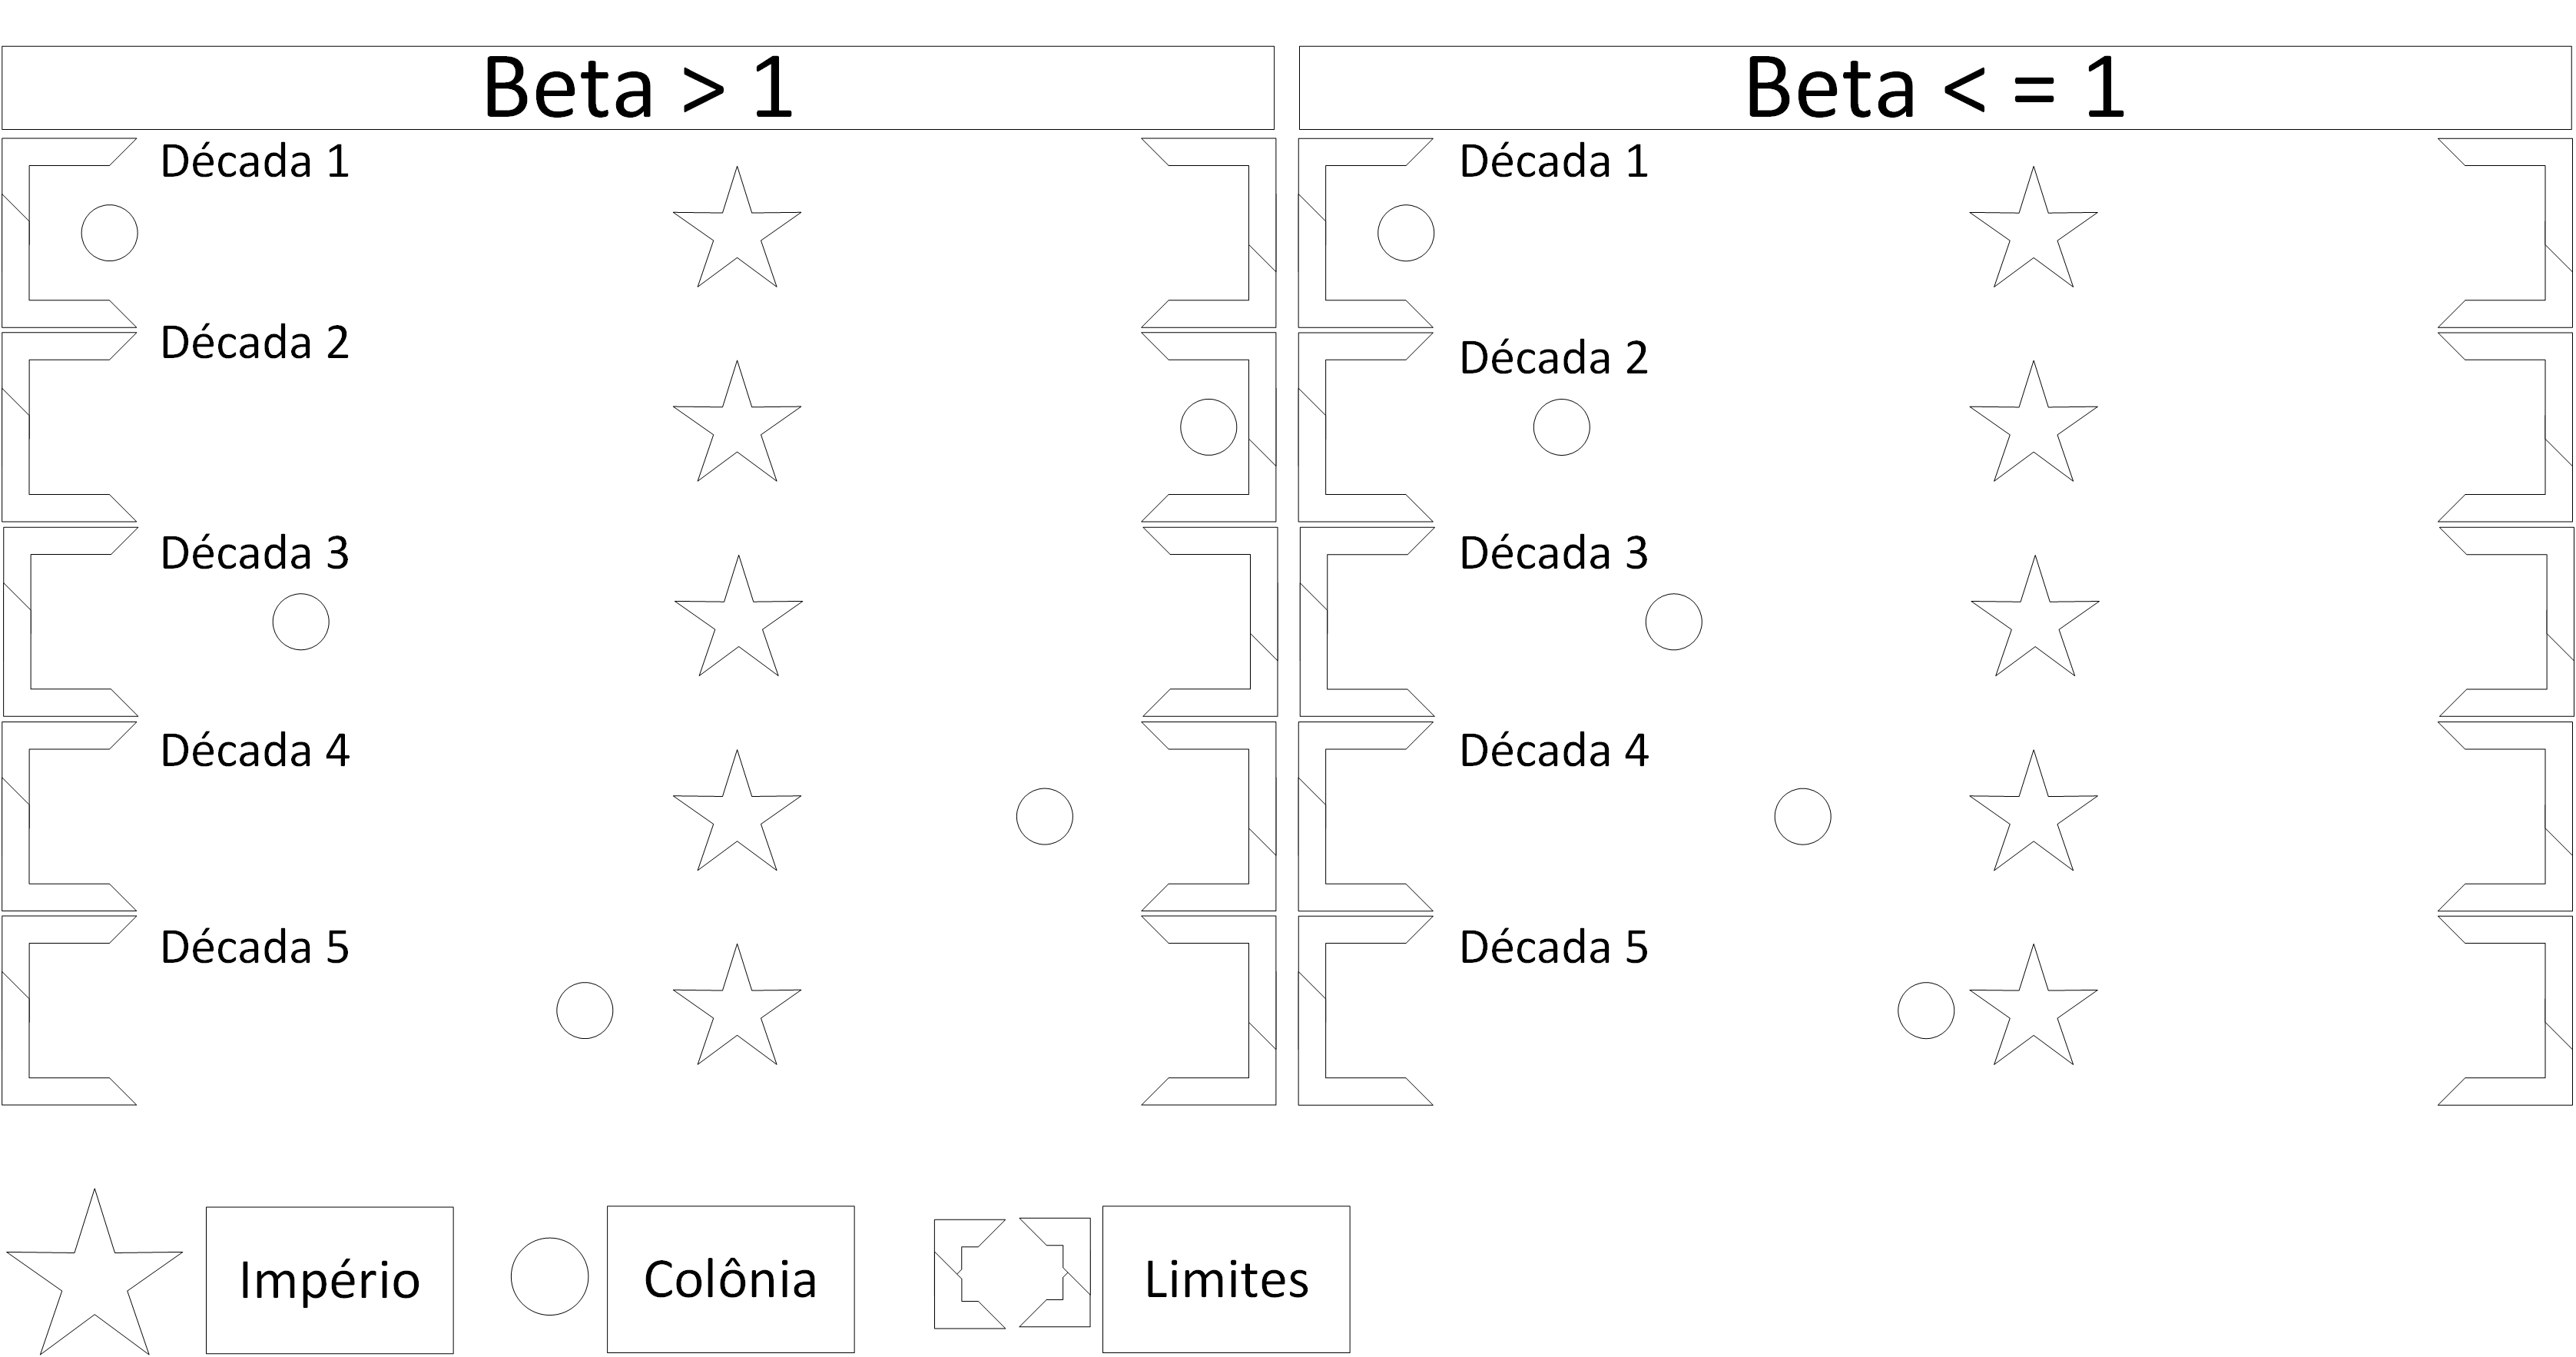
\includegraphics[scale=0.5]{Figuras/Ilustrations-BetaComparison.png}
	\caption{Comparação $\beta$ \textless 1 e $\beta$ \textgreater 1}
	\label{fig:Ilustrations-BetaComparison}
\end{figure}

Para que se tenha uma busca mais diferenciada, e que explore pontos mais diferenciados ao redor do país imperialista, ainda há a adição de um valor aleatório de desvio na direção do movimento , como mostrado na Figura \ref{fig:Ilustrations-ColonyEmpireMoveWithDistortion}. \(\theta\) é um outro valor aleatório de distribuição uniforme (ou qualquer outra que seja apropriada a situação), tal que seus limites sejam inversos e de mesma intensidade Gama, como:

\begin{equation}
\label{eq:ica8}
\theta = URand(-\gamma, \gamma)
\end{equation}

Onde \(\gamma\) é o parâmetro de ajuste de desvio da direção original. Sendo assim, a nova posição da colônia pode ser entendida como um ponto aleatório proporcional a distância entre esta colônia e seu imperialista, que explora as redondezas do império limitando-se na distância e com a adição de um ruído para a exploração mais dinâmica do espaço de busca.

\begin{equation}
\label{eq:ica9}
\text{Posição} (t+1) = \text{Posição}(t) + x + \theta
\end{equation}

\begin{figure}[h]
	\centering	
	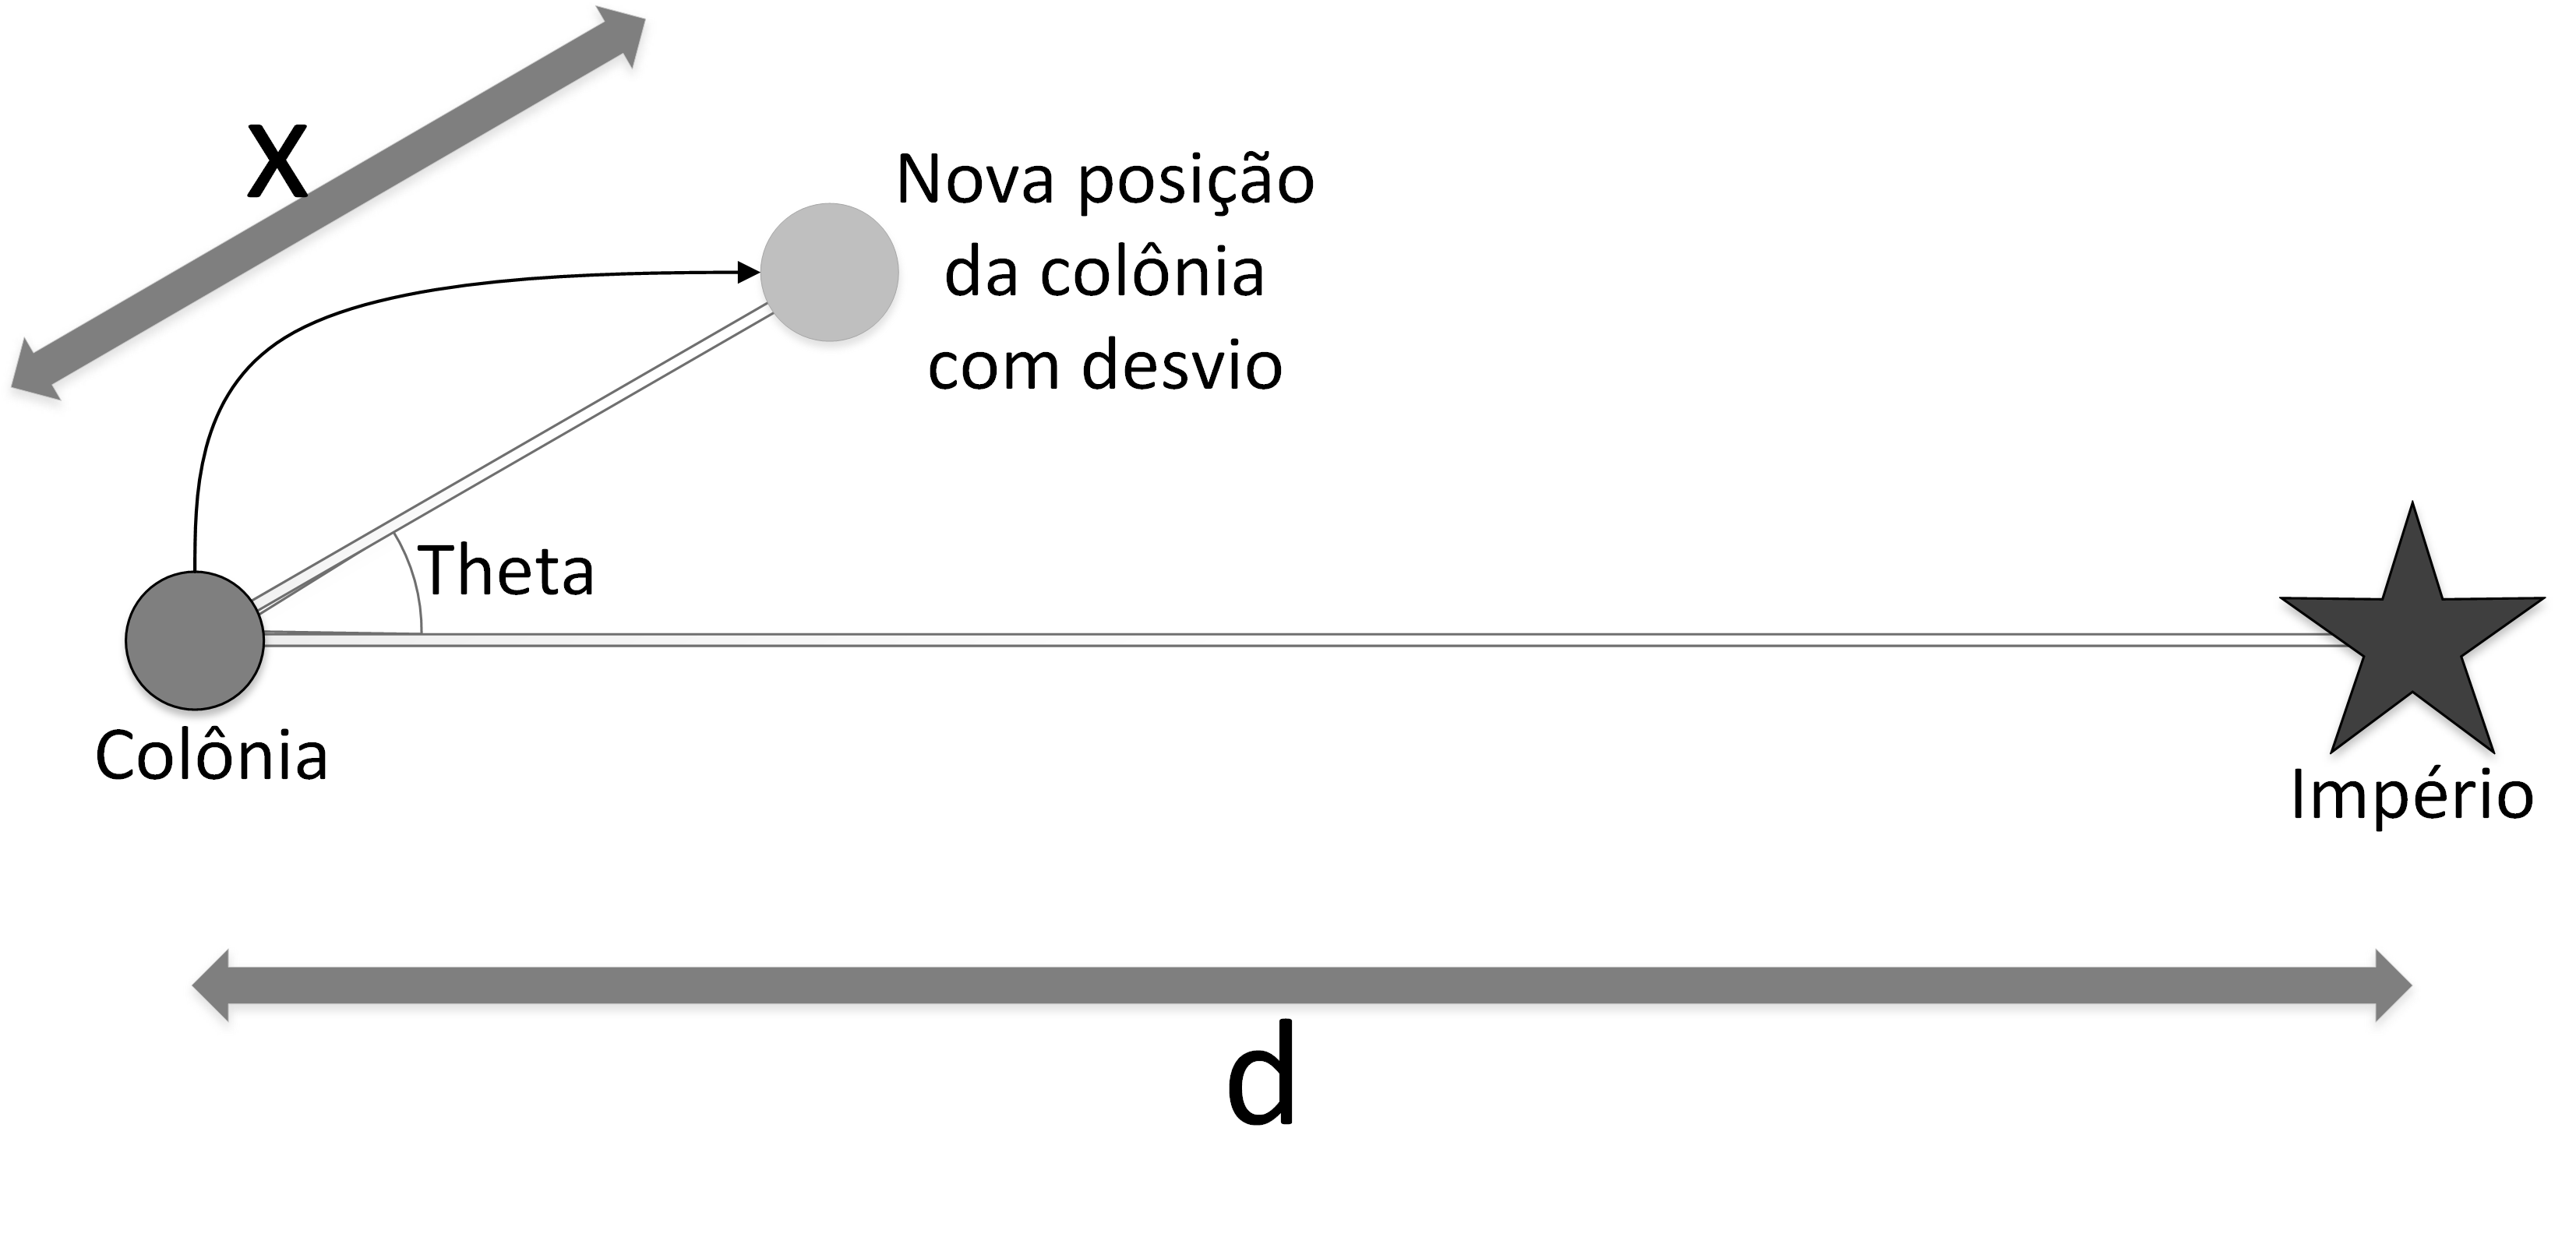
\includegraphics[scale=0.5]{Figuras/Ilustrations-ColonyEmpireMoveWithDistortion.png}
	\caption{Movimento da colônia para seu imperialista com desvio de direção}
	\label{fig:Ilustrations-ColonyEmpireMoveWithDistortion}
\end{figure}

Este processo de movimentação é executado para todas as colônias de cada país imperialista, assim que todas as colônias terminam sua movimentação, ainda é possível haver o que é chamado de processo de revolução colonial, ou apenas revolução, que é uma operação muito semelhante a operação de mutação no AG, onde todas as características (valores do vetor país) da colônia são geradas novamente de forma aleatória.

A segunda etapa, seguindo o fluxograma, faz a verificação dentre todos os imperialistas se uma de suas colônias possui características melhores que seu país imperialista, assim a colônia passa a ser o país imperialista tomando todas as colônias deste antigo imperialista em questão e inclusive, tornando este país imperialista uma colônia. Situações como esta ocorrem quando a colônia ao mover em direção ao seu país imperialista acaba se posicionando em um local onde suas características passam a apresentar um custo menor que o custo de seu país imperialista, como pode ser visto na Figura \ref{fig:Ilustrations-ColonialRevolution}. Nesta mesma figura, observa-se o movimento de colônias em direção ao seu país imperialista (quadro 1), e quando uma colônia passa por uma posição melhor que a de seu país imperialista (quadro 2), ela altera a sua cor e inicia o processo de tomada do império para si, se tornando o novo império, assimilando as colônias do antigo império e consequentemente transformando este antigo imperialista em uma colônia (quadro 3). Posteriormente, observa-se que as colônias passam a se movimentar em direção a este novo imperialista (quadro 4).

\begin{figure}[h]
	\centering	
	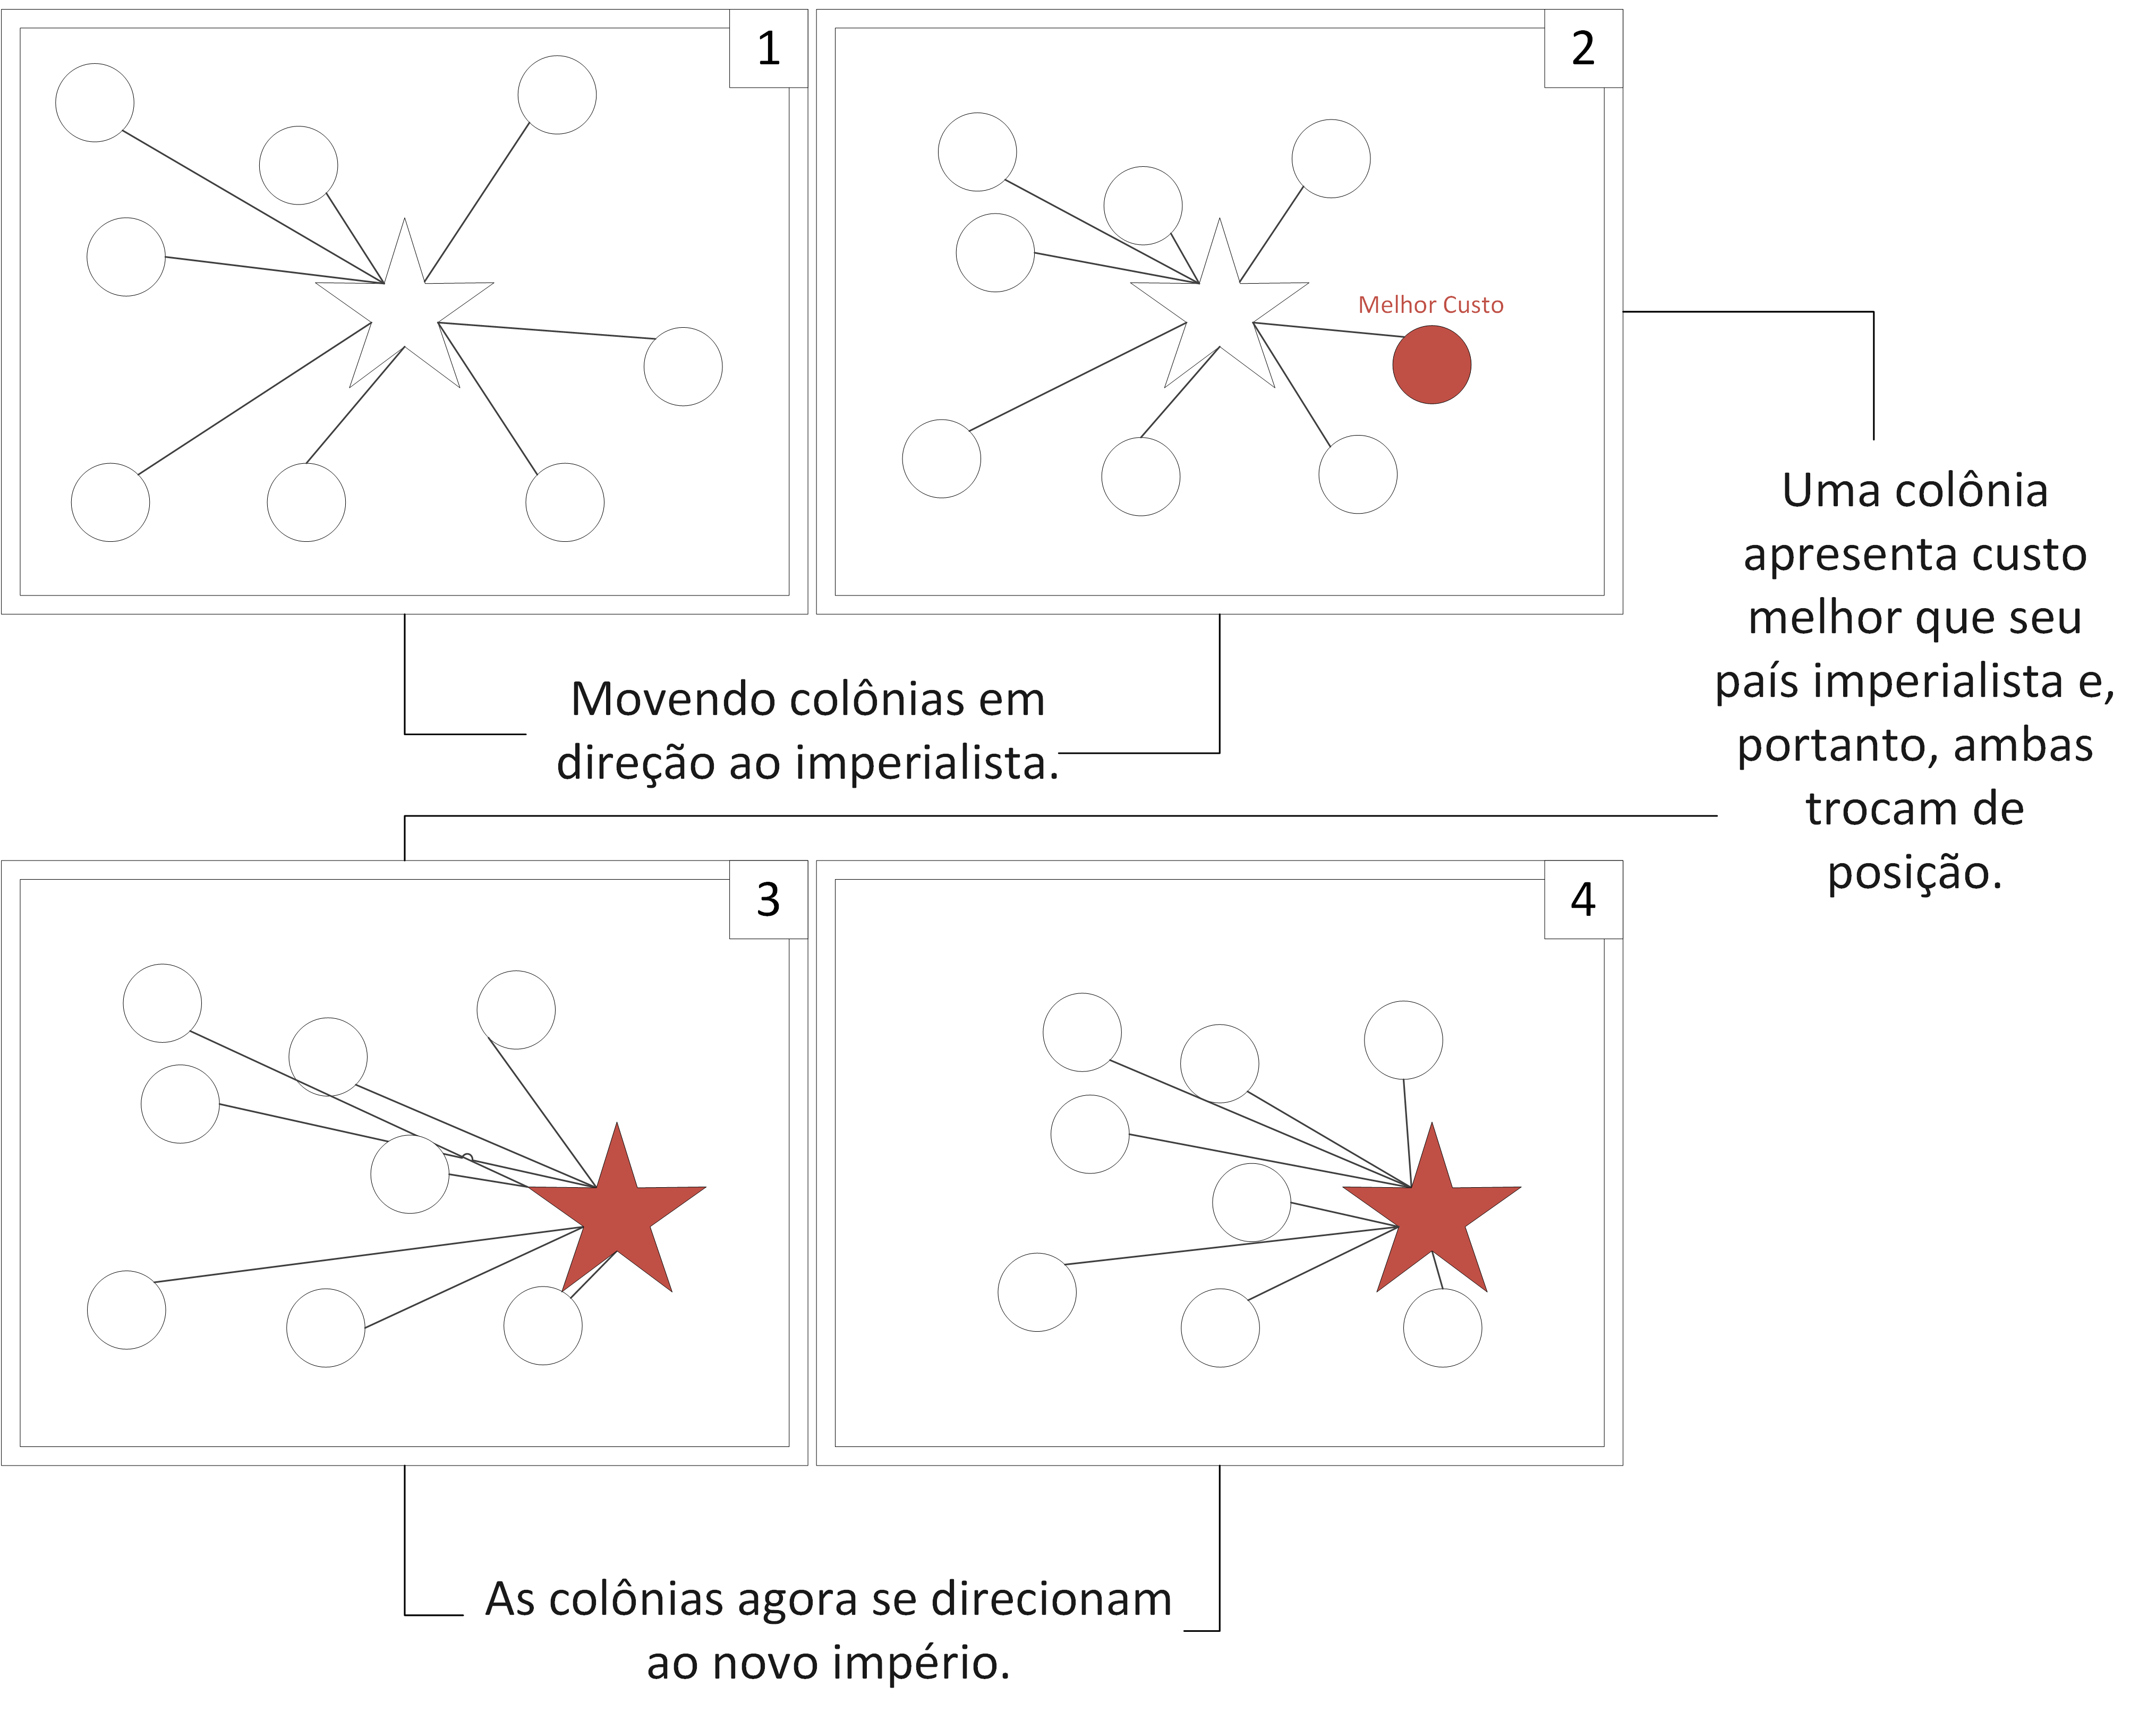
\includegraphics[scale=0.5]{Figuras/Ilustrations-ColonialRevolution.png}
	\caption{Tomada de império por colonia}
	\label{fig:Ilustrations-ColonialRevolution}
\end{figure}

Em seguida, o próximo passo, após as trocas entre impérios e colônias (caso existam), é o cálculo de todos os custos totais dos impérios, que também leva em consideração o valor do custo de suas colônias. Assim, define-se custo total de um império, como sendo a soma entre o custo do país imperialista mais uma porção da média dos custos das colônias pertencentes a este império, definido pela equação \ref{eq:ica10}:

\begin{equation}
\label{eq:ica10}
T.C.n =   Custo(Imperialista n) + \\
 \epsilon \cdot \text{Média}(Custo(Colonias do \text{império} n))
\end{equation}

No qual T.C.n é o custo total do enésimo imperialista, \(\epsilon\)  é o valor que define o quanto a média dos custos das colônias do enésimo império influenciará no custo total, sendo \(\epsilon\) menor que 1. O cálculo do custo total de um império é usado para calcular o poder de um império durante a competição imperialista. Assim, quando usa-se um valor muito baixo para \(\epsilon\) o poder do império será definido basicamente pelo custo do país imperialista, e quando aumenta-se este valor, os custos das colônias passam a ter uma maior influência no poder do império, o qual implica diretamente na competição imperialista, ou seja, se o império tem um custo baixo, porém as suas colônias tem custos muito altos, se \(\epsilon\) for baixo, este império tem maiores chances de ganhar uma competição imperialista do que se este valor de \(\epsilon\) fosse um valor mais alto.

A partir deste ponto inicia-se a competição imperialista, que se resume em selecionar a colônia mais fraca do império mais fraco e colocá-la sob o comando de um império que tenha a maior afinidade para tê-la. Assim, a competição imperialista é uma forma de aumentar o poder dos melhores impérios e diminuir o poder dos piores impérios. O império com mais chances de tomar uma colônia para si é aquele com maior poder dentre os impérios competidores, porém não é sempre que o império mais poderoso adquire a colônia em jogo, lembrando que quem adquire a colônia é aquele que tem maior afinidade para tê-la, e não maior poder. Assim, para definir o país com maior afinidade de possessão durante a competição imperialista, usa-se os valores de custo total dos impérios, calculados no passo anterior, para calcular o custo total normalizado, como mostra a equação \ref{eq:ica11}:

\begin{equation} 
\label{eq:ica11}
N.T.C.n = T.C.n - max(T.C.i)
\end{equation}

Sendo \(N.T.C.n\) o valor normalizado do custo total do enésimo império, \(T.C.n\) o custo total do enésimo império e \(max(T.C.i)\) o máximo valor dentre todos os custos totais. Assim que se calculam todos os custos normalizados, calcula-se as probabilidades de possessão de cada imperialista como mostra a equação \ref{eq:ica12}:

\begin{equation} 
\label{eq:ica12}
P_{pn} = \left| \frac{N.T.C.n}{\sum_{i=1}^{N_{imp}}N.T.C.i} \right| 
\end{equation}

Com estes valores de probabilidades de possessão para cada império, cria-se o vetor \(P\), apresentado pela equação \ref{eq:ica13}:

\begin{equation} 
\label{eq:ica13}
P = [P_{p1}, P_{p2}, ..., P_{pN_{imp}}] 
\end{equation}

Cria-se também o vetor \(R\), com o mesmo tamanho de \(P\) porém preenchido com valores aleatórios distribuídos uniformemente e limitados entre 0 e 1, tal como mostra a equação \ref{eq:ica14}:

\begin{equation} 
\label{eq:ica14}
R = [r1, r2, ..., rN_{imp}]; r1, r2,..., rN_{imp} \sim  U(0,1)  
\end{equation}

Finalmente, para definir qual será o império vencedor, que por sua vez irá tomar a colônia para si, cria-se o vetor de diferenças \(D\) de representado pela equação \ref{eq:ica15}:

\begin{equation} 
\label{eq:ica15}
D = P - R = [P_{p1}-r1, P_{p2}-r2, ..., P_{pN_{imp}}-rN_{imp}] 
\end{equation}

Os índices dos vetores \(P\), \(R\) e \(D\) representam os índices dos impérios. Assim, o índice de \(D\) que possuir o maior valor dentre os demais valores representará o império que de fato irá tomar a colônia para si. Observa-se ainda, que por meio destes cálculos não necessariamente será o país com maior poder quem irá vencer a competição e tomar a colônia para si. Mas este terá uma chance maior, e de forma proporcionalmente distribuída, de tomá-la.  

Assim que a colônia mais fraca do império mais fraco é passada para o vencedor da competição imperialista, é feita uma verificação dentre todos os impérios, que elimina aqueles impérios que não mais possuem colônias, e portanto não mais participarão das competições imperialistas e entram em colapso. O fato de eliminar o império assim que ele não possua mais colônias é só um critério que define o colapso, porém outros fatores podem fazer um império colapsar, de modo que as colônias deste tenham que ser distribuídas para os demais impérios.

O último passo do Fluxograma é a verificação das condições de parada para decidir se finaliza o algoritmo ou se repete os passos a partir do movimento das colônias para seus imperialistas. As condições de parada podem ser diversas, como número máximo de iterações (ou décadas, contextualizando), valor de custo atingido, etc. Entretanto a condição de parada ideal para convergência do ICA (verificada a cada década) deve ocorrer quando restar apenas um império e todos os demais países forem colônias pertencentes ao país imperialista. Ao considerar um cenário ideal, no qual existe apenas um império, e todas as suas colônias se situam na mesma posição de seu país imperialista, não existirá diferença nenhuma entre as colônias, e a única diferença existente entre as colônias e o império serão seus títulos.Assim, a condição de parada ideal para o ICA, em uma situação normal(não ideal), seria esperar que reste apenas um império, e ainda, se preciso, pode-se também esperar para que todas as colônias se movimentam para a posição de seu país imperialista, refinando ainda mais a solução.










\section{A operação de convolução e convolução de imagens}
   
A convolução é um operador matemático formal assim como a operação de soma ou subtração. Tal operação é uma operação linear, que é executada sobre duas funções dadas e resulta em uma terceira, a qual será a área super posicionada das mesmas em função do deslocamento existente entre ambas.

Este operador tem sido amplamente utilizado em diversas áreas, sendo aplicado em áreas como processamento de sinais e imagens, circuitos elétricos, telecomunicações, probabilidades e estatísticas, entre outras, visando a filtragem e detecção de características em sinais ou imagens. No caso deste trabalho aplica-se a convolução para o processamento de imagens (também conhecido como filtragem no domínio do espaço), sobre uma metodologia diferente do convencional, descrita mais adiante, de modo que os resultados da aplicação de um filtro \(g\), que \emph{convoluciona} por toda uma imagem \(f(t)\) sejam os mais próximos possíveis de uma previsão futura de expansão, \(f'(t+1)\), tal que \(f(t+1)\) seja uma imagem um período à frente de \(f(t)\).

Em A Origem e História da Convolução \cite{dominguez2010origin}, são apresentadas diversas definições matemáticas sobre a operação de convolução, e neste caso, o que nos interessa é a convolução discreta, que tem seu conceito aplicado no processamento de imagens como:

\begin{citacao}
Seja \(\{x_{i}\}\) e \(\{y_{i}\}\) duas sequências de valores reais ou complexos tal que \(-\infty \textless i \textless \infty\). A convolução discreta dessas sequências resulta em uma nova sequência definida pela expressão:
\[\begin{split}
\sum_{n=-\infty}^{\infty}x_{n} \cdot y_{i+-n}, \\ \small{-\infty \textless i \textless \infty}
\end{split}\] 
Nota-se que se uma sequência, \(\{x_{i}\}, i = 0, 1, ..., n1-1\), tem um número de termos \(n1\) e a sequência \(\{y1\}, i = 0, 1, ... n2-1\), tem um número de termos \(n2\), então a convolução discreta dessas duas sequencias deve ser escrita na forma:
\[\begin{split}
\sum_{n=0}^{i} x_{n} \cdot y_{i+-n}, \\i = 0, 1, ..., n1-1; \\n = n1 + n2 - 1
\end{split}\]
A convolução discreta dessas duas sequências finitas que tem \(n1\) e \(n2\) termos respectivamente, e resulta em uma nova sequencia contendo \(n1+n2-1\) termos. \cite{dominguez2010origin}
\end{citacao}

Este conceito mostra como a convolução é aplicada sobre duas sequências de valores resultando no valor final do somatório, portanto, a técnica aplicada neste trabalho utiliza a convolução para fazer a filtragem espacial de imagens, que gera de uma nova imagem \(g\) a partir da convolução dos pontos de uma imagem \(f\) sobre uma matriz ou filtro de convolução \(m\).

Esta técnica de filtragem espacial, então, pode ser representada como sendo uma transformação da imagem, de forma ponto a ponto, que dependem do valor de um determinado ponto e do valor dos pontos vizinhos na imagem original. Assim o ponto a ser filtrado terá um valor referente à região que ele se encontra na imagem original. 

Assim, a filtragem por convolução pode ser efetuada como mostra a expressão \ref{eq:g=fm}:

%\[g = f * m\]
\begin{equation}
\label{eq:g=fm}
g = f * m
\end{equation}

sendo:

\begin{itemize}
\item \(g\) a imagem resultado da filtragem, 
\item \(f\) a imagem original, 
\item \(m\) a máscara ou filtro de convolução e 
\item \(*\) o operador de convolução.
\end{itemize}

Para se obter a imagem \(g\), executa-se a operação de convolução de \(m\) sobre todos os pontos da imagem \(f\), assim, um ponto \((x,y)\) da imagem \(g\) é calculado como mostra a equação \ref{eq:convolucao}:
	
%\[
\begin{equation}
\label{eq:convolucao}
\begin{split}
g(x,y) = \
\sum_{i=\left\lfloor\frac{O}{2}\right\rfloor}^{\left\lfloor\frac{O}{2}\right\rfloor} \
\sum_{j=\left\lfloor\frac{O}{2}\right\rfloor}^{\left\lfloor\frac{O}{2}\right\rfloor}  f(x+i, y+j) \cdot m(i,j)
\end{split}
\end{equation}
%\]

Sendo \(O\) a ordem da máscara de convolução, que tem altura e largura iguais a \(O\) e \(i\) e \(j\) os iteradores sobre a máscara. Tal operação de filtragem pode ser ilustrada como mostra a Figura \ref{fig:Convolution}, que apresenta uma matriz \emph{m} convoluindo uma matriz \emph{f} para gerar uma matriz \emph{g}:

\begin{figure}[h]
	\centering	
	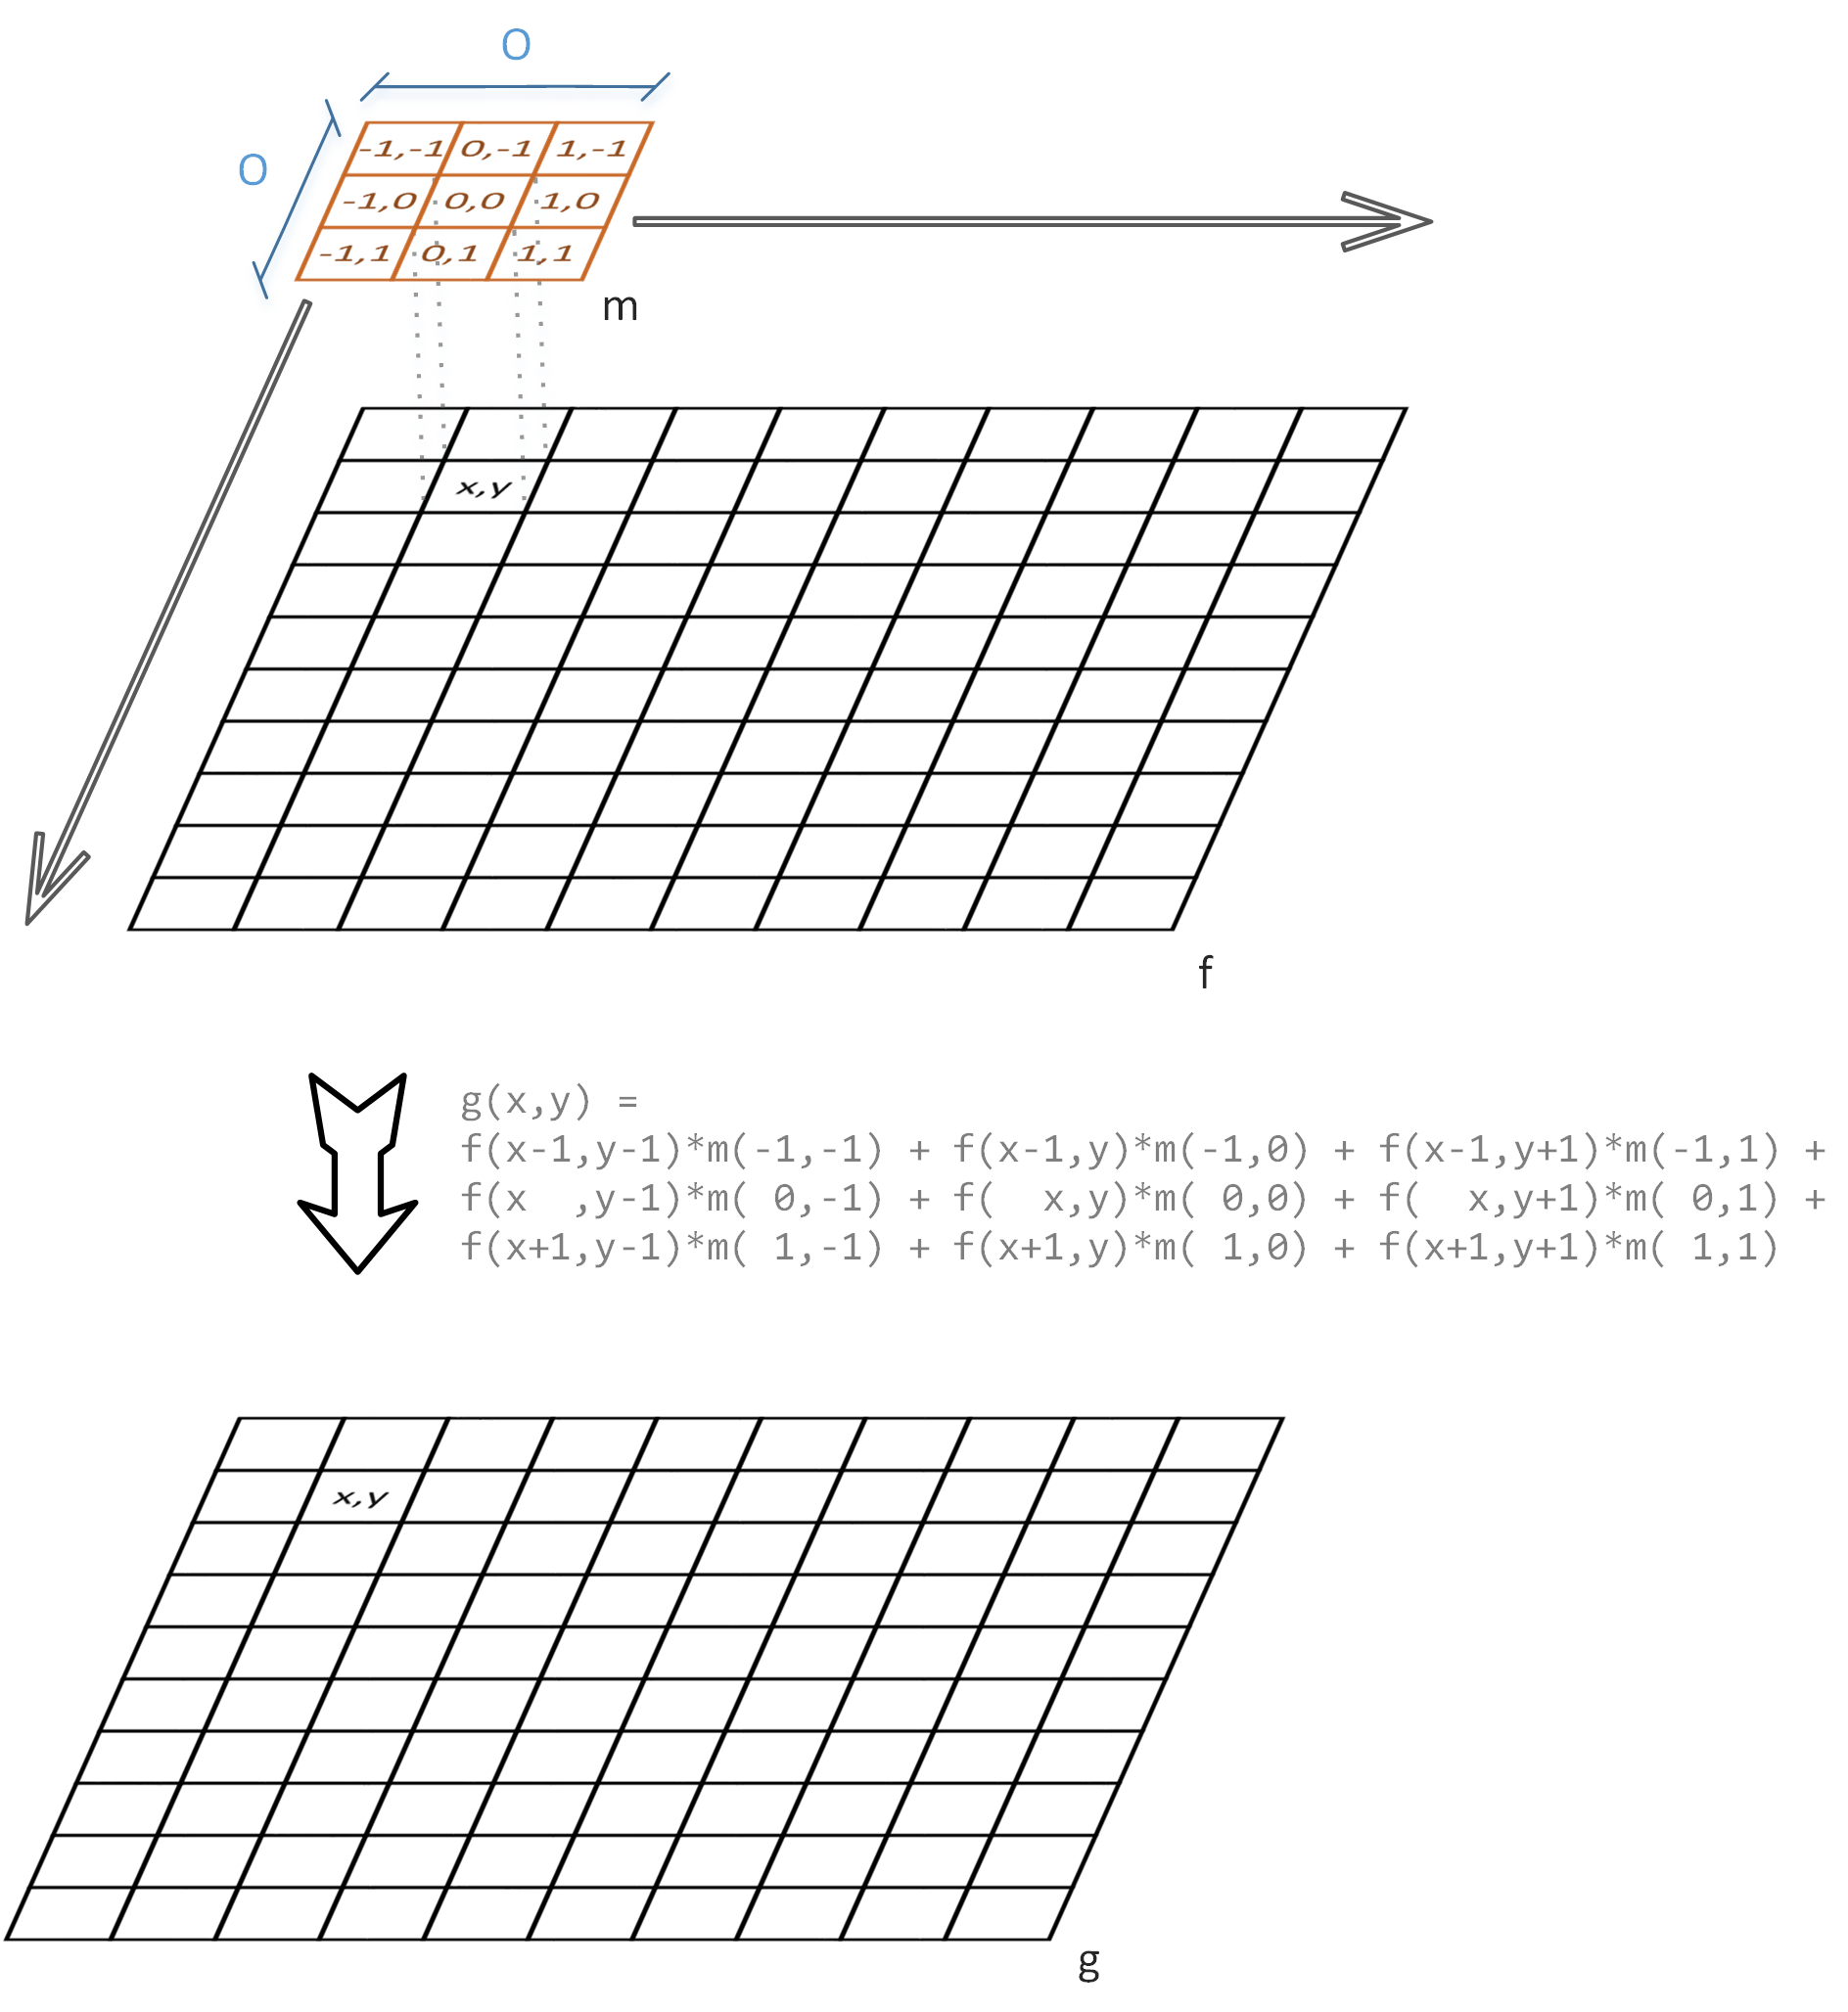
\includegraphics[scale=0.55]{Figuras/Convolutio.png}
	\caption{Filtragem por convolução}
	\label{fig:Convolution}
\end{figure}

Observe que o elemento central da máscara fica posicionado sobre o ponto \((x,y)\) da imagem, para que se possa calcular o ponto \((x,y)\) de \(g\) efetuando a convolução de \(f\) por \(m\). Observe ainda, que a matriz de convolução, para gerar toda a imagem \(g\), percorrendo todos os pontos de \(f\)  e aplicando a convolução ponto a ponto. E note também, no cálculo de \(g(x,y)\) na Figura \ref{fig:Convolution}, que a convolução faz a soma das multiplicações entre os elementos da matriz \(m\) com a imagem \(f\), de modo que os índices dos elementos estejam sempre nas mesmas posições, ou seja, o ponto \((x,y)\) de \(f\) será multiplicado pelo elemento \((0,0)\) de \(m\), o ponto \((x+1,y)\) de \(f\) será multiplicado pelo elemento \((1,0)\) de \(m\), e assim por diante.

Com isso pode-se elaborar um algoritmo para processar uma imagem \(f\) sob uma matriz de convolução \(m\) dadas, ambas na forma de matriz de valores, de modo a se gerar uma imagem resultante \(g\) a partir da convolução da matriz \(m\) sobre a imagem \(f\), como mostrado a seguir no algoritmo \ref{alg:Convolution}:

\begin{algorithm}[H]
\SetAlgoLined
\KwData{
\\m \(\Rightarrow\) Matriz de convolução.
\\f \(\Rightarrow\) Imagem Inicial.
\\w \(\Rightarrow\) Largura da imagem em pixels.
\\h \(\Rightarrow\) Altura da imagem em pixels.
\\o \(\Rightarrow\) Ordem da matriz de convolução.

}
\KwResult{g - Imagem resultante da convolução de m sobre f }
Inicializar g como uma nova matriz[w][h] com zeros\;
\Para{$x \leftarrow $0 \KwTo $w$}
{
  \Para{$y \leftarrow $0 \KwTo $h$}
  {
    OffsetX - x - (int)(o/2)\;
    \Para{$i \leftarrow $0 \KwTo $o$}
    {
      OffsetY = y - (int)(o/2)\;
      \Para{$j \leftarrow $0 \KwTo $o$}
      {
        \Se{! (OffsetX < 0 OU\\ OffsetX >= w OU\\ OffsetY < 0 OU\\ OffsetY >= w) }
        {
        g[x][y] = g[x][y] + f[OffsetX][OffsetY] * m[i][j]\; 
        }
        OffsetY++\;
      }
      OffsetX++\;
    }
  }
}
\caption{Algoritmo de convolução de imagens}
\label{alg:Convolution}
\end{algorithm}

O algoritmo apresentado é o mais simples possível, e é otimizado para a rápida execução da tarefa, portanto ele não apresenta alguns recursos extras, que geralmente aparecem em algoritmos de convolução de imagens digitais, como a adição de um fator de multiplicação \(r\) e de um fator de soma \(baias\), que altera a imagem resultante g gerada, de modo que o fator \(r\), geralmente dentro do intervalo \([0,1]\), multiplica todos os elementos da imagem após o cálculo do ponto, e analogamente, o fator de soma \(baias\), que soma todos os elementos calculados da imagem resultante \(g\).  Tais fatores, no caso deste trabalho não são necessários, pois a matriz de convolução será gerada a partir de um algoritmo evolutivo, que já integra tais valores nos próprios elementos da matriz de convolução, caso seja necessário. Outro fato interessante a se analisar é que este algoritmo utiliza muito processamento e é diretamente dependente do tamanho da imagem e da máscara de convolução, pois, tomando como exemplo uma matriz de tamanho 5x5 e uma imagem 100x100, haverão 250000 multiplicações e 250000 somas para gerar a imagem final como resultado da convolução entre a imagem e a matriz.

Os filtros ou matrizes de convolução, quando aplicados sobre imagens, utilizando a técnica mostrada anteriormente tem diversas aplicações, como nas áreas de pré-processamento, remoção de ruídos, segmentação, suavização, detecção de bordas etc. No caso deste trabalho, é apresentado uma nova aplicação, dentro de uma metodologia que leva a geração de uma imagem resultante a qual representará uma imagem futura a partir de imagens anteriores.


\section{Previsor Espacial de Mapas de Densidade}

Este trabalho propõe o desenvolvimento de uma aplicação chamada Previsor Espacial de Mapas de Densidade (P.E.M.D.) para que sejam gerados mapas de previsão utilizados como fatores essenciais em planejamentos de expansão.

O previsor Espacial de Mapas de Densidade utiliza como entrada um conjunto de dados dispostos em uma tabela, de modo que tais dados representem fatores de Posição geográfica, Data, Tipo e Quantidade. os fatores Tipo e Quantidade podem ser utilizados de forma combinada para alterar o valor de intensidade cada quadrícula do histórico de mapas a ser gerado, possibilitando assim que tal histórico de mapas de quadrículas seja utilizado para gerar mapas de previsão futura.

A aplicação consiste nas etapas de:
\begin{itemize}
	\item Criação do histórico de mapas de quadrículas,
	\item Regionalização do histórico do mapa de quadrículas,
	\item Otimização dos parâmetros de previsão utilizando o ICA,
	\item Utilização dos parâmetros de previsão para geração de previsões futuras utilizando o último mapa do histórico de mapas como mapa base das previsões.
\end{itemize}    

Um dos grandes desafios do previsor é a criação da função de previsão, que neste caso é baseada na operação de convolução, e que utilizará um mapa de quadrículas e um conjunto de fatores de previsão para gerar um mapa previsto de um período à frente do mapa base.

O conjunto de fatores de previsão utilizado pela função de previsão é otimizado pelo ICA, que em sua função de avaliação, faz uma análise do histórico do mapa de quadrículas criando uma espécie de regressão linear espacial, minimizando as diferenças entre os períodos com o ajuste dos fatores de previsão.



\chapter{Desenvolvimento do ICA Genérico}
\label{Desenvolvimento}


Neste capítulo são detalhados como os conceitos relacionados ao ICA apresentados previamente foram desenvolvidos. Suas melhoras, adaptações e correções são apresentadas de forma a facilitar a organização e desempenho computacional. 

Foram propostas modificações no ICA de forma a produzir uma implementação que possui maior desempenho na busca pela solução ideal para o problema proposto, fazendo com que suas operações possam ser processadas em paralelo, corrigindo um problema de valores aleatórios não proporcionais (o Problema da Dimensionalidade) quando se usa dimensões de intervalos variados e a generalização na modelagem dos problemas.

%A formulação do ambiente apresenta como os dados são trabalhados, formando os mapas de quadrículas para serem processados pelo ICA, e como o problema de previsão é modelado em uma função de avaliação do ICA, onde todo o processo é descrito na seção \ref{Inicialização do ICA}, que usa uma aplicação diferenciada, combinando matrizes de convolução e fatores de ponderação.




\section{ICA Orientado a Objetos}
\label{ICA Orientado a Objetos}

Esta seção contém todas as melhorias efetuadas no ICA, independente de seu uso para previsão, sendo que tais modificações são genéricas para qualquer aplicação. Então esta seção foca em duas formas de otimização, sendo a primeira, a organizacional, impactando diretamente no desenvolvimento, e a segunda, as alterações para desempenho. Visto que originalmente, o ICA não é implementado, é apenas conceituado, e ainda tem-se que a função de previsão baseada em convolução é uma operação muito pesada, forçando que se desenvolva uma implementação que apresente desempenho satisfatório e seja genérica para que diversos testes possam ser realizados.

Assim, o desenvolvimento do ICA de forma orientada a objetos é classificada como uma modificação organizacional, e é focada nos quatro pilares da orientação a objetos:
\begin{itemize}
\item Abstração, que é responsável por fazer a separação dos elementos presentes no ICA por identidade, propriedades e métodos, e neste caso criando-se 4 elementos:

\begin{itemize}
\item Classe ‘ImperialistCompetition’, que define todo o processo evolucionário da competição imperialista desde sua inicialização até o término da repetição presente no algoritmo, obedecendo as condições de parada. Esta é a principal classe do sistema que faz o uso de todos os outros elementos descritos abaixo, dando sentido a cada um deles.
\item Classe ‘Country’, que por sua vez descreve as propriedades e métodos que um país possuirá na competição imperialista, é esta classe que define, após a inicialização se um país é um imperialista ou uma colônia, além de armazenar e gerenciar o vetor país(citado nos conceitos do ICA).
\item Interface ‘IFitness’, que traz a definição do problema a ser abordado pelo os países em competição.
\item  Classe abstrata ‘StopCondition’, que representa uma condição de parada. Na qual após uma competição imperialista, uma ou mais condições de parada podem ser verificadas em sequência, parando a execução do algoritmo. Assim pode-se ter uma condição de parada por número máximo de décadas, ou por número de imperialistas competindo sendo verificadas ao mesmo tempo. A condição que primeiro for verificada como verdadeira irá parar a execução do ICA.
\end{itemize}
 
\item Encapsulamento, que torna o desenvolvimento mais flexível, de modo que novas implementações sejam mais fáceis de criar ou modificar, pois mantém as partes da implementação separadas, como se fosse blocos ou módulos, os quais apenas precisam ser conectados para que funcionem. 
Permite também o isolamento de propriedades privadas, sendo estas acesso apenas por métodos específicos \emph{getters} e \emph{setters}. Permitindo a adição de propriedades que facilitam o acesso aos atributos específicos de um elemento, ou validando valores inseridos ou alterados por agentes externos ao escopo do objeto.

\item Herança, usada para modelar elementos mais complexos definidos de acordo com o modelo do problema, permitindo a extensão da classe \emph{Country} para adicionar propriedades ou métodos. Além de que ao se usar em combinação com polimorfismo pode alterar o comportamento de métodos através de sobrescrita.

\item Polimorfismo, que permite referenciar tipos mais abstratos, os quais apenas definem o comportamento dos elementos concretos que os implementa. Neste caso, a definição da interface \emph{IFItness} e da classe abstrata \emph{StopCondition}, é a aplicação do polimorfismo no ICA, que faz com que diversos problemas possam ser criados separadamente e sem que seja preciso alterar o funcionamento interno do  ICA.
A sobrescrita de métodos da classe \emph{Country}, quando estendida para alteração de comportamento e/ou funcionalidade, também é uma utilização de polimorfismo, uma vez que o ICA continua usando apenas os métodos e propriedades da classe base \emph{Country} (mesmo se sobrescritos), e não de sua extensão, que provavelmente será usada pela implementação da interface \emph{IFitness} em questão.
\end{itemize}

Uma vez definido como será o desenvolvimento no aspecto de organização, aplicando os conceitos de orientação a objetos, os próximos passos devem focar no aspecto de otimização da aplicação para a obtenção das respostas em um período de tempo aceitável. Assim, foram definidas duas alterações, na qual uma delas não implica diretamente na alteração do funcionamento do ICA, sendo estas, a implementação do ICA de forma que este processe as funções de aptidão de forma paralelizada, e uma outra modificação que altera como as colônias se relacionam com seus países imperialistas durante o processo evolutivo.

Dentro da segunda categoria de  modificações, relacionadas à performance, são propostas algumas alterações no funcionamento de como algumas etapas do ICA são efetuadas e também são propostas algumas funcionalidades adicionais que podem ocorrer entre as etapas básicas do ICA.

Uma modificação que resultou em um bom aumento de precisão do ICA para soluções complexas é a alteração da forma com que uma colônia se movimenta para seu país imperialista, a qual fora denominada de “movimento refinado”, e que é uma otimização feita no algoritmo do ICA para que ele explore o espaço de busca de uma forma mais homogênea, controlando os ruídos (durante a movimentação) e mantendo a velocidade e precisão de convergência. Outra abordagem, denominada “visão imperial distorcida”, também foi utilizada com o mesmo intuito, buscando outra abordagem de movimento aleatorizado, apresentando bons resultados e com uma capacidade de ser combinado com o primeiro.

As funcionalidades de Revolução Colonial e União Imperial são duas adições mencionadas por \cite{roche2011imperialist} que implicam na alteração do comportamento dos países e impérios, responsáveis por aumentar a velocidade de convergência do ICA para uma solução ótima. 

A Revolução Colonial é uma funcionalidade muito semelhante a mutação presente no algoritmo genético canônico, e por sua vez, neste contexto, faz com que um país que seja colônia de um país imperialista, tenha todos os seus atributos aleatorizados de forma que o ICA se torne capaz de evitar máximos/mínimos locais. A revolução colonial tem uma chance de ocorrer, podendo esta chance cair ou aumentar ao longo das décadas.

A União Imperial é uma funcionalidade adicionada para aumentar a velocidade de assimilação de um império por outro e evitar que dois impérios ocupem as mesmas posições. Assim, deve existir um limiar de união, que quando um império chegar próximo o suficiente de outro, inicia-se o processo de união, onde o império mais fraco é englobado pelo império mais forte.
    
    
    
    
    
    
    
    
    
    
    
\subsection{Modelagem e desenvolvimento}
\label{Modelagem e desenvolvimento}

O desenvolvimento de problemas que venham a utilizar de técnicas de inteligência artificial são implementados a partir de seu modelo matemático, que geralmente não são otimizados computacionalmente, ou ainda, que não são nem modelados apropriadamente para serem ótimos em determinado ambiente computacional. No ambiente em questão existem diversos tipos de linguagens de programação, as quais possuem diversas características, que por sua vez, definem as qualidades e desvantagens desta linguagem. As linguagens de programação e suas características principais são diferenciadas em sua essência pelos paradigmas de programação, onde os quatro principais paradigmas são bem caracterizados por  \cite{normark2013overview}. Tais paradigmas são uma forma de classificar determinada linguagem de acordo com seu estilo de programação e classifica suas características principais como apresentado na Figura \ref{fig:Ilustrations-Paradigms}.


\begin{figure}[h]
	\centering	
	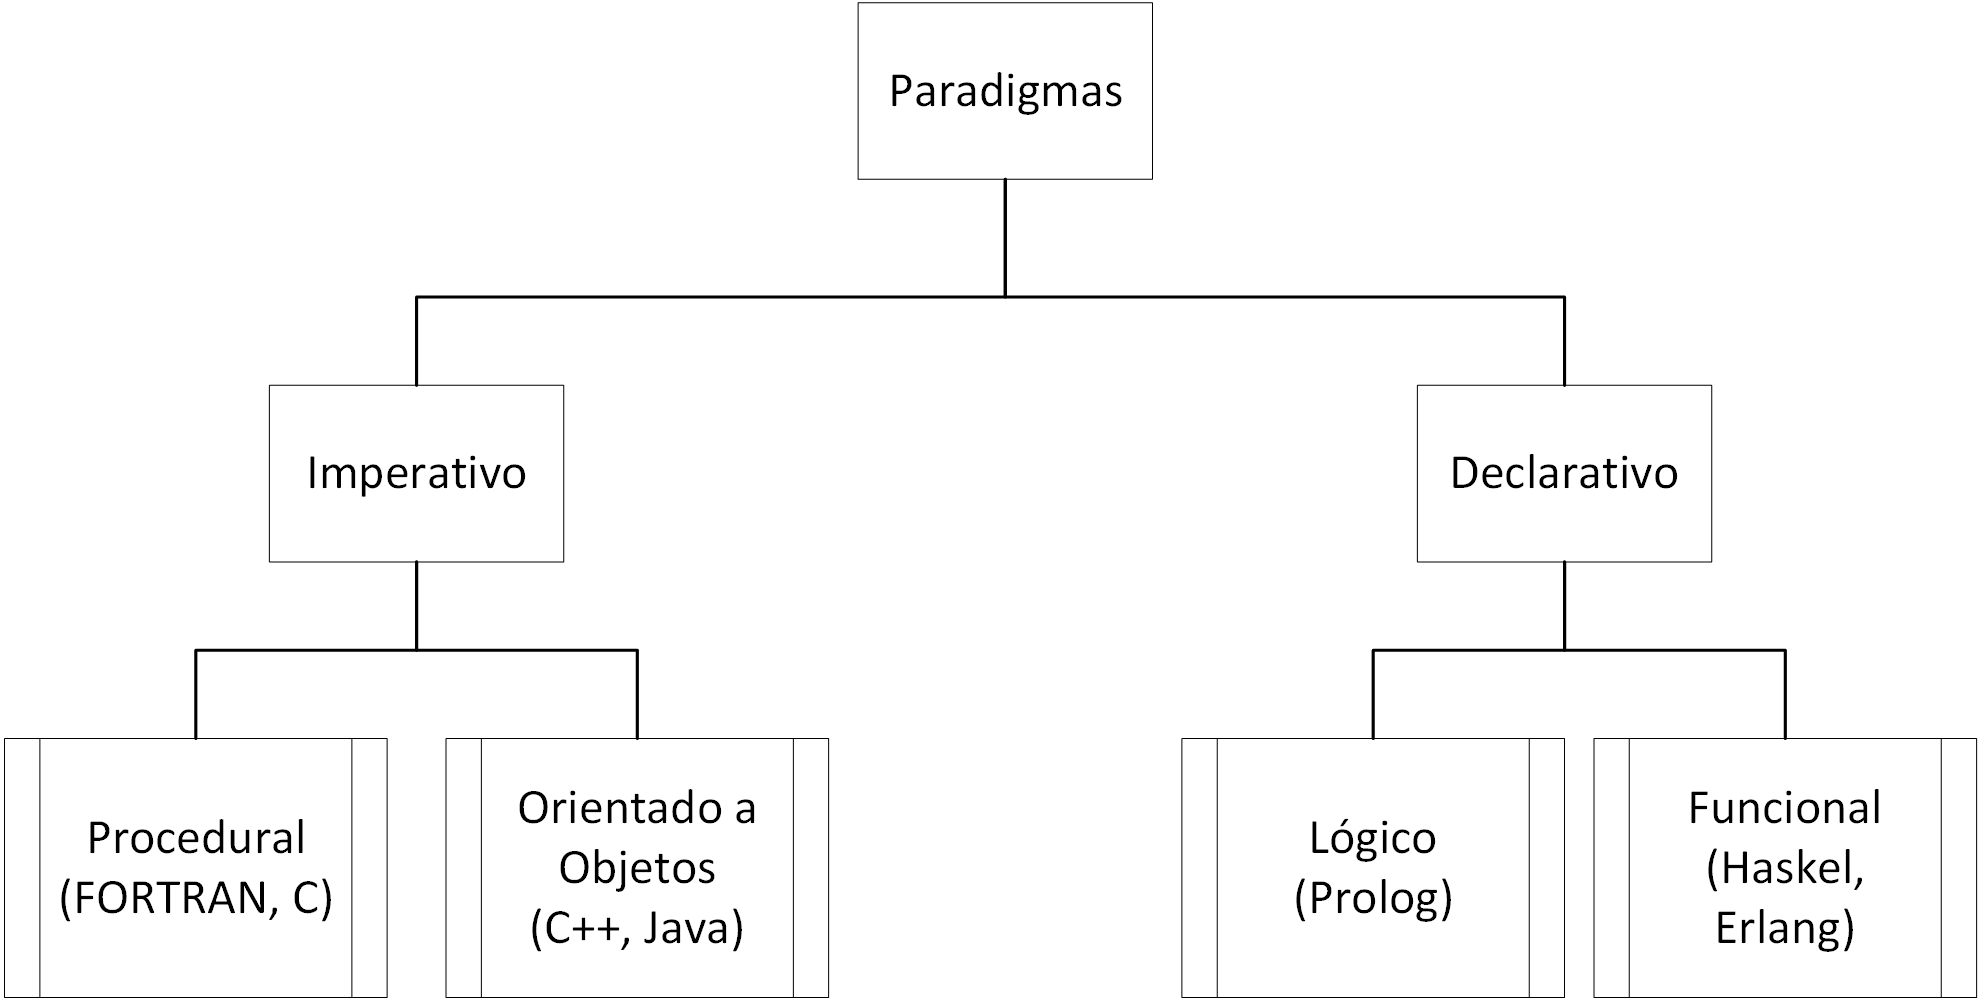
\includegraphics[scale=0.7]{Figuras/Ilustrations-Paradigms.png}
	\caption{Paradigmas de programação}
	\label{fig:Ilustrations-Paradigms}
	\end{figure}


Para a modelagem de problemas de inteligência artificial, geralmente são escolhidas linguagens que pertencem aos paradigmas funcionais, porém, tais linguagens possuem mais limitações que as pertencentes ao paradigma imperativo, seja este limite em relação ao controle sobre o sistema ou aos dados. Este é um dos motivos de se ter escolhido uma linguagem pertencente ao paradigma imperativo (em sua essência) para o desenvolvimento deste trabalho. Como pode-se ver na Figura \ref{fig:Ilustrations-Paradigms} o paradigma imperativo divide-se em dois principais sub paradigmas, o procedural e o orientado a objetos (paradigma escolhido como melhoria para o desenvolvimento). 

A linguagem de programação escolhida para o desenvolvimento do ICA pertence ao paradigma de programação imperativo orientado a objetos em sua maior parte, porém algumas de suas características se encaixam nas funcionalidades do paradigma declarativo funcional, que são funcionalidades como delegados (\emph{Delegate} - os quais permitem que funções sejam tratadas como objetos de primeira ordem, o que nada mais é do que um tipo seguro de ponteiro de função), inferência de tipo (que faz dedução automática de um tipo de dados), funções anônimas (ou abstrações lambdas), linguagem de consulta integrada LINQ, entre outros. Estes recursos são capazes de otimizar e imitar algumas das características utilizadas pelo paradigma declarativo funcional dentro de uma linguagem imperativa orientada a objetos. Assim, pode-se dizer que a linguagem é multi paradigmas, pois possui características de orientação a objetos, que permite tratar os campos de dados como objetos manipuláveis através de métodos pré-definidos, e permitindo também que a implementação faça o uso dos seus quatro conceitos mais importantes: abstração, encapsulamento, polimorfismo e herança, além de usufruir dos conceitos que não fazem parte do paradigma imperativo, que também estão presentes na linguagem. 

O algoritmo do ICA foi desenvolvido neste trabalho utilizando a linguagem de programação C\#. Como descrito acima, esta linguagem multi paradigmas permite o uso dos conceitos de orientação a objetos, que possibilitam uma forma diferente de organizar o problema. Tendo em mente que para se desenvolver uma solução que resolva o problema proposto, será necessário efetuar diversos testes com diversos modelos. A aplicação dos conceitos de orientação a objetos será imprescindível para organizar e manter o desenvolvimento de forma ágil e resiliente. A modelagem do ICA orientado a objetos foi particionado em 4 etapas básicas, na qual cada uma referência a um dos 4 pilares da Orientação a Objetos.

Primeiramente, foi pensado em como separar os elementos básicos do ICA em objetos de forma que tais objetos pudessem ser caracterizados de forma a ter uma identidade única, seus próprios métodos e propriedades dentro do escopo em questão, abstraindo a concepção do ICA para algo mais tangível como na separação em objetos que podem ser descritos por classes (inclusive interfaces e classes abstratas). Assim, foram criadas duas classes, uma classe abstrata e uma interface, sendo elas:
\begin{itemize}
\item Classe \emph{ Country }
\item Classe \emph{ImperialistCompetition  }
\item Interface \emph{IFitness}
\item Classe Abstrata \emph{ StopCondition}
\end{itemize}

A classe \emph{Country} (Figura \ref{fig:ClassesICA-Country})  representa um país do ICA, sendo este colônia ou império, e é semelhante a um indivíduo no GA. O país possui o conjunto de atributos que serão usados pela função de avaliação de modo que esta função de avaliação calcule um custo para este país, sendo este valor de custo armazenado na própria classe. Esta classe ainda armazena atributos que definem se o país é um país imperialista ou se ele é uma colônia. Logo, para que se possa manusear melhor o país, independente de sua posição política, existe um valor que representa dois estados, dependendo do que o país possa ser, colônia ou império. Se este país for uma colônia, este valor representará o número do império a que este país pertence. Se este país for um império, este valor será o índice do vetor de impérios ordenados por custos presente na classe \emph{ImperialistCompetition} descrita logo abaixo.

Durante o desenvolvimento foi pensado que poderiam ser criadas mais duas classes, sendo estas a classe Colônia e a classe Imperialista, que derivariam da classe \emph{Country}, porém não foram criadas por dois motivos: (1) A concepção de uma classe Colônia e uma classe Imperialista que derivassem da classe \emph{Country} não teriam nem propriedades e nem métodos que as diferenciassem da classe, sendo estas diferentes apenas suas identidades (OBS: a classe imperialista até poderia possuir um vetor para as colônias que controla, mas seria redundante e aumentaria a complexidade no controle das operações efetuadas pelo ICA). (2) O segundo motivo é referente ao impacto da implementação destas duas classes, que necessitaria de muito mais lógica para manuseio dos objetos, sendo que o foco não é implementar uma abstração tão afundo da ideia original, mas sim uma implementação de baixa complexidade, que faça com que o sistema seja simples de ser mantido e testado. 

\begin{figure}[h]
	\centering	
	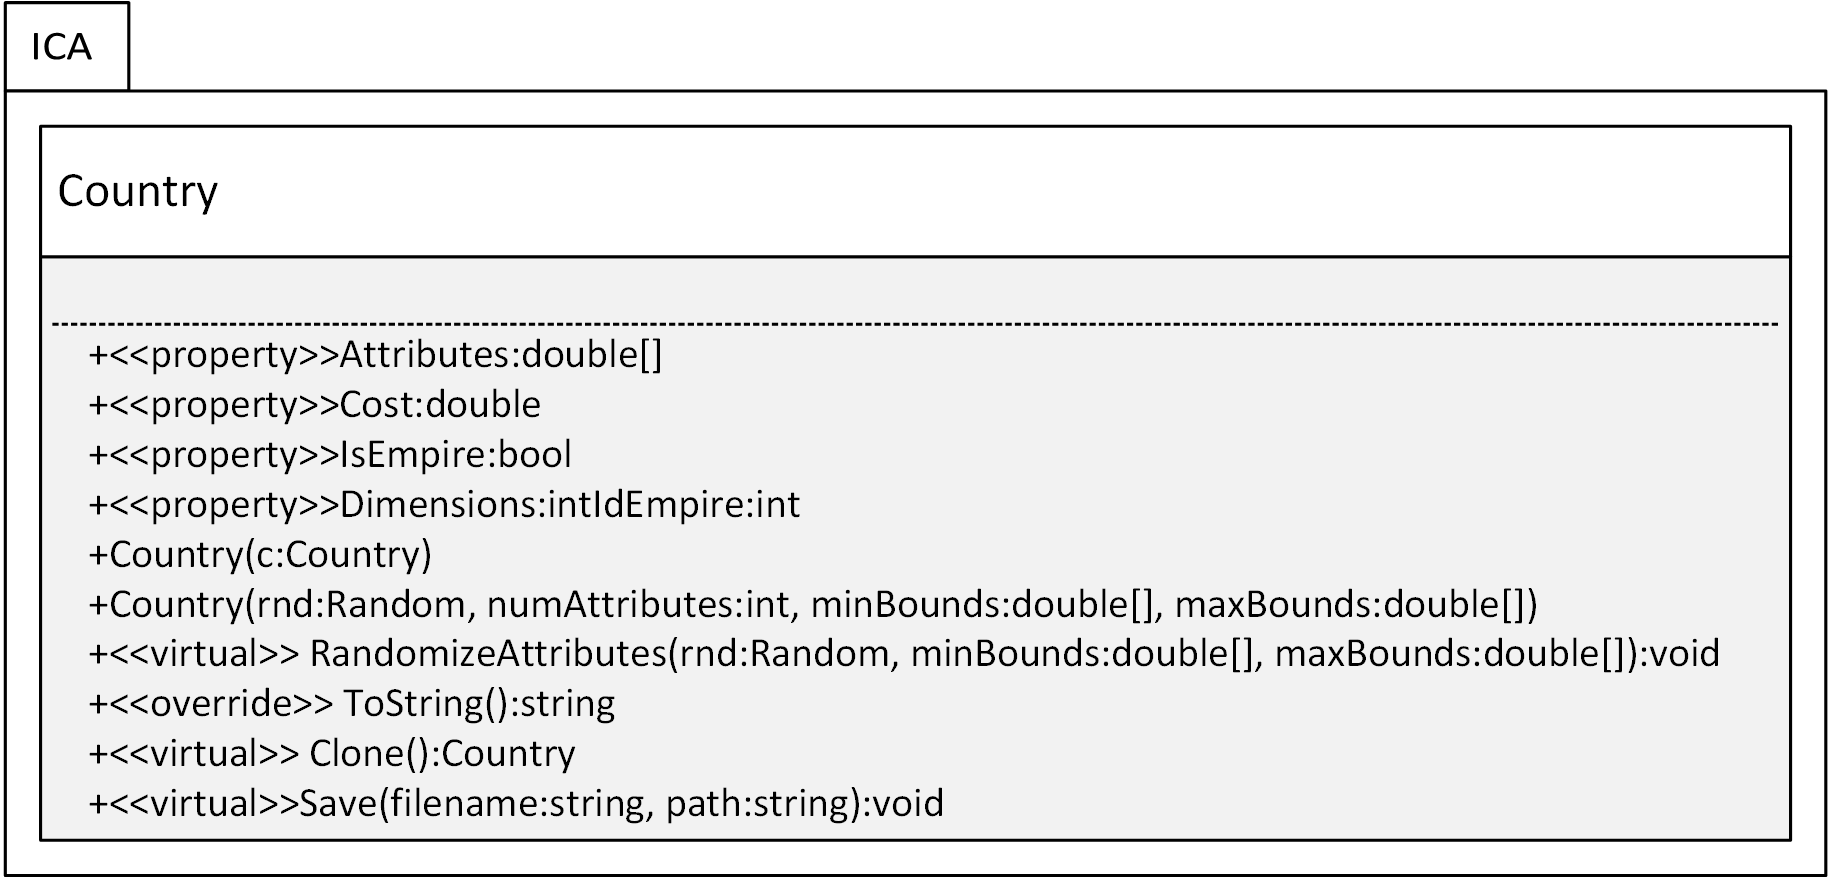
\includegraphics[scale=1]{Figuras/ClassesICA-Country.png}
	\caption{Classe Country}
	\label{fig:ClassesICA-Country}
	\end{figure}

Para completar a modelagem da classe \emph{Country}, foram adicionados alguns métodos essenciais para o funcionamento genérico do ICA. Dois destes métodos são construtores para a classe, no qual o primeiro recebe como parâmetro um outro objeto do tipo \emph{Country} e inicializa seus valores fazendo uma cópia direta de todos os atributos do parâmetro, o segundo construtor inicializa todos os seus valores com valores padrão da linguagem, porém recebe diversos parâmetros, nos quais são basicamente usados para chamar o método \emph{RandomizeAttributes} logo após a inicialização dos valores da classe. Dentre os quatro métodos restantes o método \emph{ToString} é o mais simples, apenas retornando uma cadeia de caracteres formatada dos valores da classe, o método \emph{Clone} faz uma cópia do objeto em questão usando o primeiro construtor, o método \emph{Save} grava em um arquivo de texto com os dados do objeto, e por fim, o método \emph{RandomizeAttributes} faz uma randomização dentro dos valores \emph{minBounds} e \emph{maxBounds} para todos os atributos do indivíduo. 


Nota-se ainda que os métodos \emph{RandomizeAttributes} e \emph{Clone} são virtuais, isto indica que quando a classe \emph{Country} for derivada (usando o conceito de herança), estes métodos poderão ser substituídos por novos com uma lógica diferenciada (OBS: o construtor da classe também pode ser sobrescrito e ter sua lógica alterada em um cenário de extensão da classe \emph{Country}). O fato de poder se criar uma classe tomando como base a classe \emph{Country} e mesmo assim o ICA continuar funcionando é devido à aplicação do conceito de polimorfismo aplicado na modelagem da aplicação. Neste caso, quando se implementa uma classe\emph{ Country} estendida, o ICA não é responsável por instanciar a lista de países, esta responsabilidade é do método \emph{GenerateCountries}, que deve ser implementado por classes derivadas da interface \emph{IFitness} (descrita logo abaixo). Assim, na classe \emph{Country}, foram abordados todos os quatro conceitos essenciais de orientação a objetos, mantendo uma grande flexibilidade para a utilização genérica do ICA.    

A classe \emph{ImperialistCompetition} será abordada por último, pois é nela que todos os outros componentes são interligados e é necessário que os demais estejam bem definidos. Então, continuando com a interface \emph{IFitness}, que é responsável por fazer com que os objetos que venha a implementá-la, obrigatoriamente tenham os métodos de interface implementados. Como pode-se observar na Figura \ref{fig:ClassesICA-IFitness}, de todos os métodos, o mais importante é o método \emph{Eval} e em seguida o método \emph{GenerateCountries}, descritos mais detalhadamente logo abaixo.


\begin{figure}[h]
	\centering	
	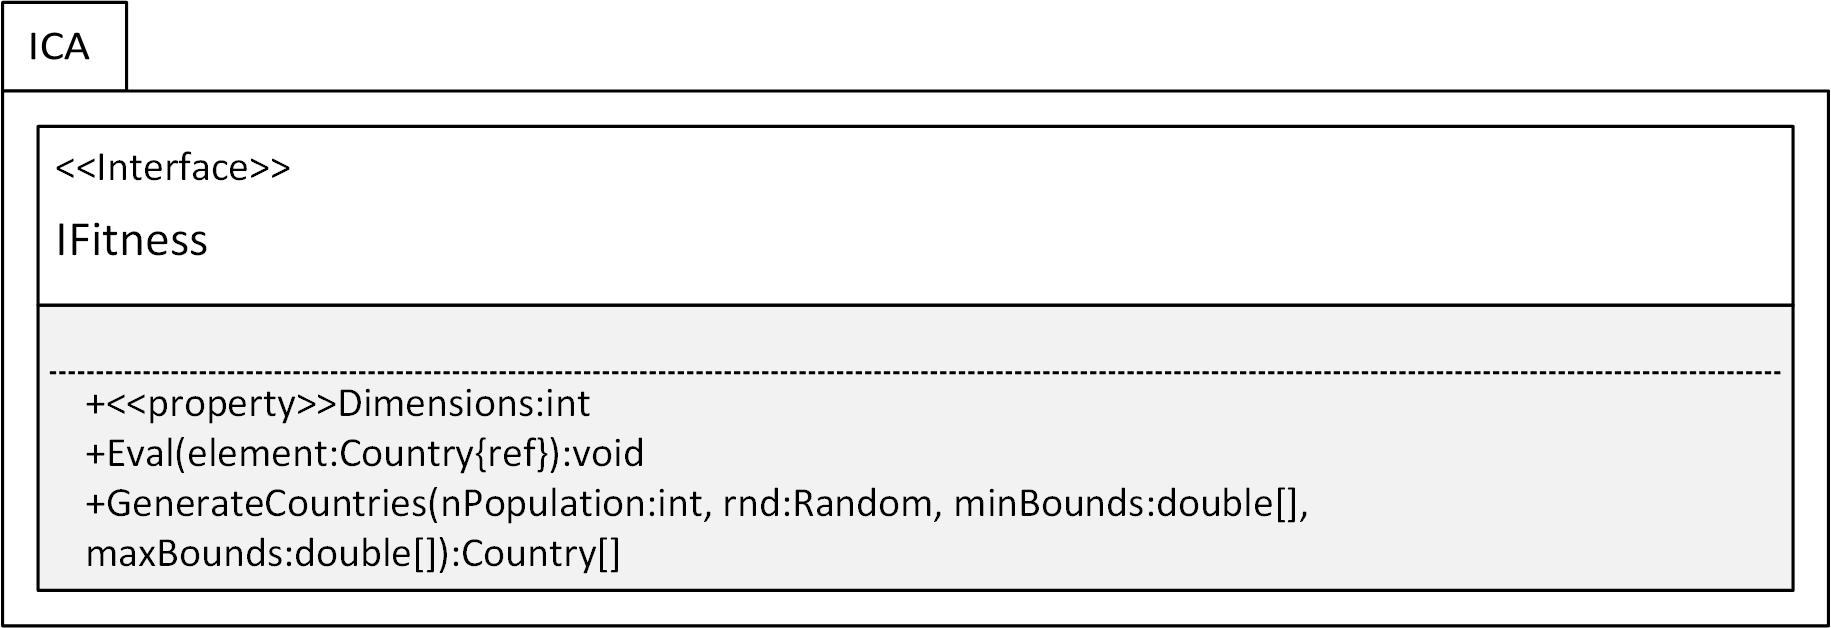
\includegraphics[scale=1]{Figuras/ClassesICA-IFitness.png}
	\caption{Interface IFitness}
	\label{fig:ClassesICA-IFitness}
	\end{figure}


O método \emph{Eval} é o mais importante, ele representa a própria função de avaliação do problema em questão e é o principal fator que levou a criação desta interface. É neste método que ocorrem os cálculos para a avaliação de cada país e consequentemente a atribuição do valor do custo calculado a cada país em questão. É essencial que seja passado como parâmetro a referência de um país para que o custo seja calculado a partir dos valores deste, e em seguida já atribuir o valor do custo a este país passado por referência. Assim, qualquer alteração ao país, que ocorra dentro da função \emph{Eval} será persistida para o objeto no escopo da classe \emph{ImperialistCompetition}, vista mais adiante que é a responsável por fazer as chamadas de avaliação dos países, desta forma evita-se múltiplas trocas de mensagens e simplifica-se o funcionamento, tanto para o processamento serial, quanto para paralela.
 
Na sequência, o segundo método, \emph{GenerateCountries}, é quem define a construção da lista de países para que o ICA possa iniciar sua execução, a lista de países pode ser iniciada normalmente, gerando-se uma lista e inicializando seus elementos, porém, a grande vantagem de se ter este método de forma explícita e obrigatória para cada problema a ser implementado é referente a liberdade de poder inicializar alguns países (ou todos) em posições privilegiadas, ou seja, se existir algum pré processamento nos dados, pode-se iniciar os países e seus atributos de forma que estes estejam próximos da solução ótima sem que se precise limitar o espaço de busca. Os parâmetros de entrada para este método são:
\begin{itemize}
\item \emph{nPopulation} - valor que representa a quantidade de países a serem criados,
\item \emph{rnd} - um objeto do tipo \emph{Random} para que a aleatorização inicial seja efetuada sem que ocorram problemas com a paralelização (discutidos no tópico sobre Paralelização),
\item \emph{maxBounds} e \emph{minBounds} -  que são as duas listas de valores representando os limites superior e inferior respectivamente para cada dimensão do problema.
\end{itemize}

Nota-se ainda uma propriedade chamada \emph{Dimensions} na interface, sendo que esta propriedade é responsável por definir o número de dimensões do problema em questão. Como visto anteriormente o valor de dimensão é que definirá o tamanho do vetor de atributos dos países, sendo este valor muito usado pelo ICA. A inserção desta propriedade para definir este valor na interface implica que a classe responsável pelo controle do algoritmo não precisa se preocupar em inicializar tal valor (pois, na maioria dos casos, seu valor dependerá da modelagem do problema). Cada problema no ICA deve ser modelado de forma que possa ter suas soluções na forma de um vetor de valores, no caso do ICA tais valores são números de ponto flutuante, sendo o número de elementos deste vetor o número de dimensões do problema.

Por fim, percebe-se que a interface \emph{IFitness} é a responsável por encapsular a lógica do problema a ser otimizado através da implementação de seus membros em uma classe separada para cada problema. Assim, cria-se um nível de abstração que separa o funcionamento do algoritmo da implementação/avaliação do problema, sendo que a classe \emph{ImperialistCompetition} deve obrigatoriamente obter os valores necessários para sua execução (Lista de países, número de dimensões do problema e chamada da função de avaliação de um país) a partir de uma implementação da interface \emph{IFitness}, porém não precisa ter informação alguma sobre como a acontece a geração da lista de países, como avaliação de um dado país ocorre ou como se define o valor de dimensões do problema etc.. Assim, quando se implementa uma função de avaliação para um dado problema, na maioria das vezes existe a necessidade de manter variáveis do problema que não fazem parte diretamente da solução, mas sim do modelo do problema. Estes valores devem estar inseridos na classe que implementa o problema, para que o ICA não precise ter suas funcionalidades principais alteradas, mantendo a aplicação genérica a qualquer problema deve-se implementar a interface \emph{IFitness} e seus métodos com o foco no problema em questão. Desta forma, o ICA se mantém genérico a qualquer solução, sendo que qualquer classe que implemente um problema diferente seja polimórfica, ou seja independente do problema em questão, o ICA apenas utilizará os métodos e propriedades expostos pela interface \emph{IFitness}, não tendo contato algum com os demais elementos da modelagem do problema.

Na metodologia do ICA foi mostrado que podem haver diversas formas de convergir um problema, porém a solução ótima geralmente se apresenta quando existe apenas um país imperialista, e este possui todas as colônias geradas inicialmente, de forma que tais colônias estejam na mesma posição em que o país imperialista se encontra. Durante a execução de alguns problemas, notou-se que a convergência para apenas um país pode levar muito tempo, ou também que pode-se atingir uma solução aceitável mesmo ela não sendo pertencente ao cenário ótimo de convergência do ICA. Assim, para que o ICA possa gerenciar diversas condições de parada para um dado problema foi pensada uma abstração que permite extrair apenas a lógica das condições de parada para fora do ICA.

A Figura \ref{fig:ClassesICA-StopCondition} apresenta a classe \emph{StopCondition}, que define como foi modelada a abstração das condições de parada. Uma condição de parada deve implementar esta classe e definir as regras de parada dentro do método \emph{VerifyBreak}, que é chamado sempre que se inicia um ciclo (ou década, contextualizando para o ICA) no algoritmo. Observa-se que diversos parâmetros são passados para este método, assim, as condições de parada mais comuns podem ser implementadas e adicionadas no ICA. Ainda existem duas propriedades na classe abstrata, a primeira, é usada apenas para definir o nome da condição de parada, para fins de análise. Já a segunda, é usada exclusivamente pelo ICA para gerenciar uma lista de diversas condições de parada que possam estar sendo verificadas em sequência. Note que tal propriedade é pública, porém possui o método \emph{set} como interno (definido pela palavra chave \emph{Internal}), o que significa que apenas a própria instância pode alterar o valor, mas qualquer um pode lê-lo (pois o seu método \emph{get} continua público).
 
\begin{figure}[h]
	\centering	
	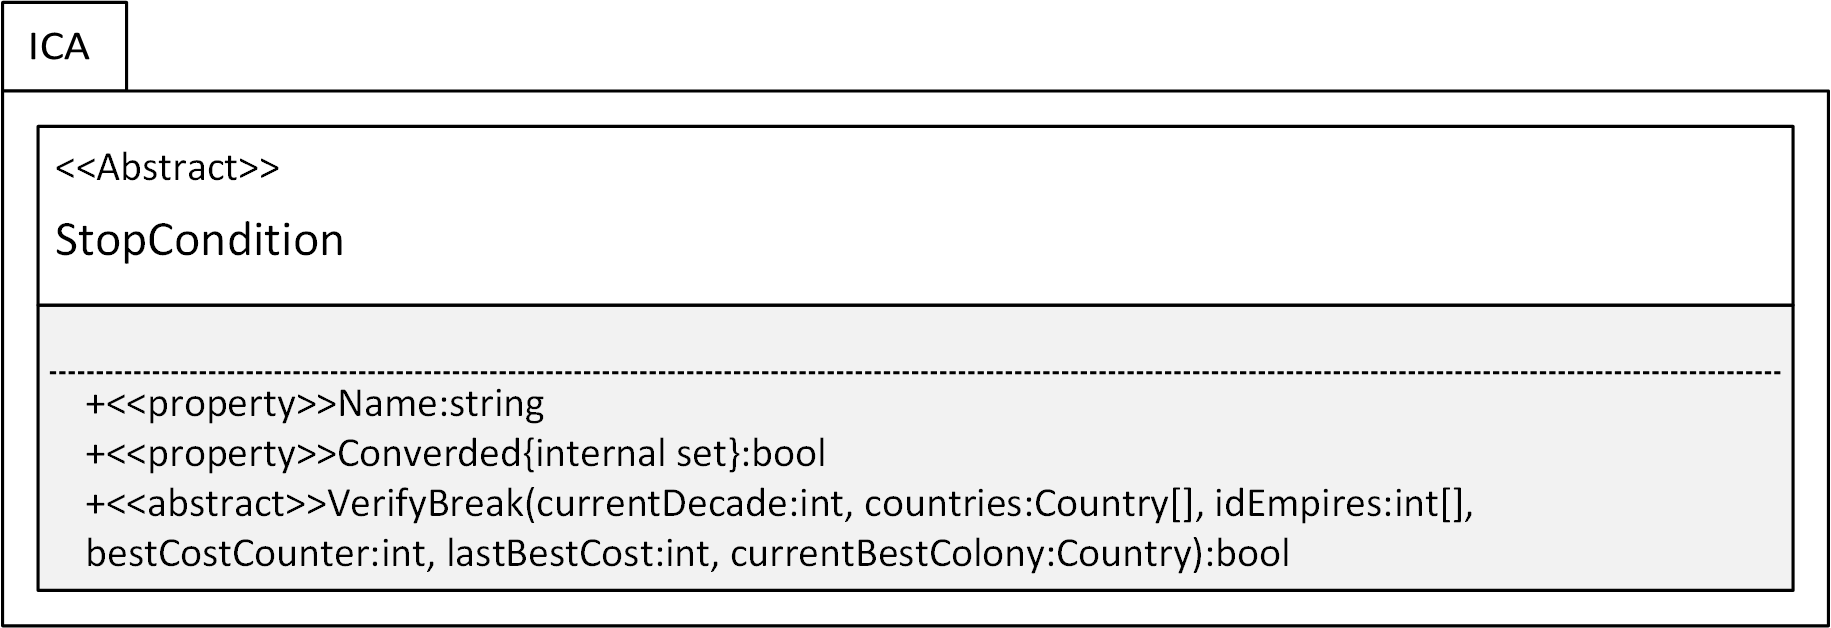
\includegraphics[scale=1]{Figuras/ClassesICA-StopCondition.png}
	\caption{Classe Abstrata StopCondition}
	\label{fig:ClassesICA-StopCondition}
	\end{figure}

A Figura\ref{fig:ClassesICA-StopConditionsImplements} define as condições de parada:
\begin{itemize}
\item Número máximo de décadas - que força parada da evolução do ICA quando um valor de iterações (décadas) for atingido. 
\item Estagnação por década - que força parada da evolução do ICA quando o valor do melhor custo da solução não se alterar durante um número de ciclos (décadas) estipulado.
\item Estagnação por porcentagem de custo - que força a parada da evolução do ICA quando o valor do melhor custo subtraído do melhor custo anterior  se manter dentro de uma variação percentual durante um número de ciclos (décadas) estipulado.
\end{itemize}
Tais condições de parada foram implementadas e inseridas na rotina de iteração do ICA, para que este possa convergir mais rapidamente para uma solução aceitável. A utilização destas condições de parada é configurável e portanto pode-se utilizar a condição padrão citada na metodologia, que apenas irá parar o algoritmo quando todas as colônias estiverem sob o poder de apenas um império de tal forma que suas posições sejam as mesmas.

\begin{figure}[h]
	\centering	
	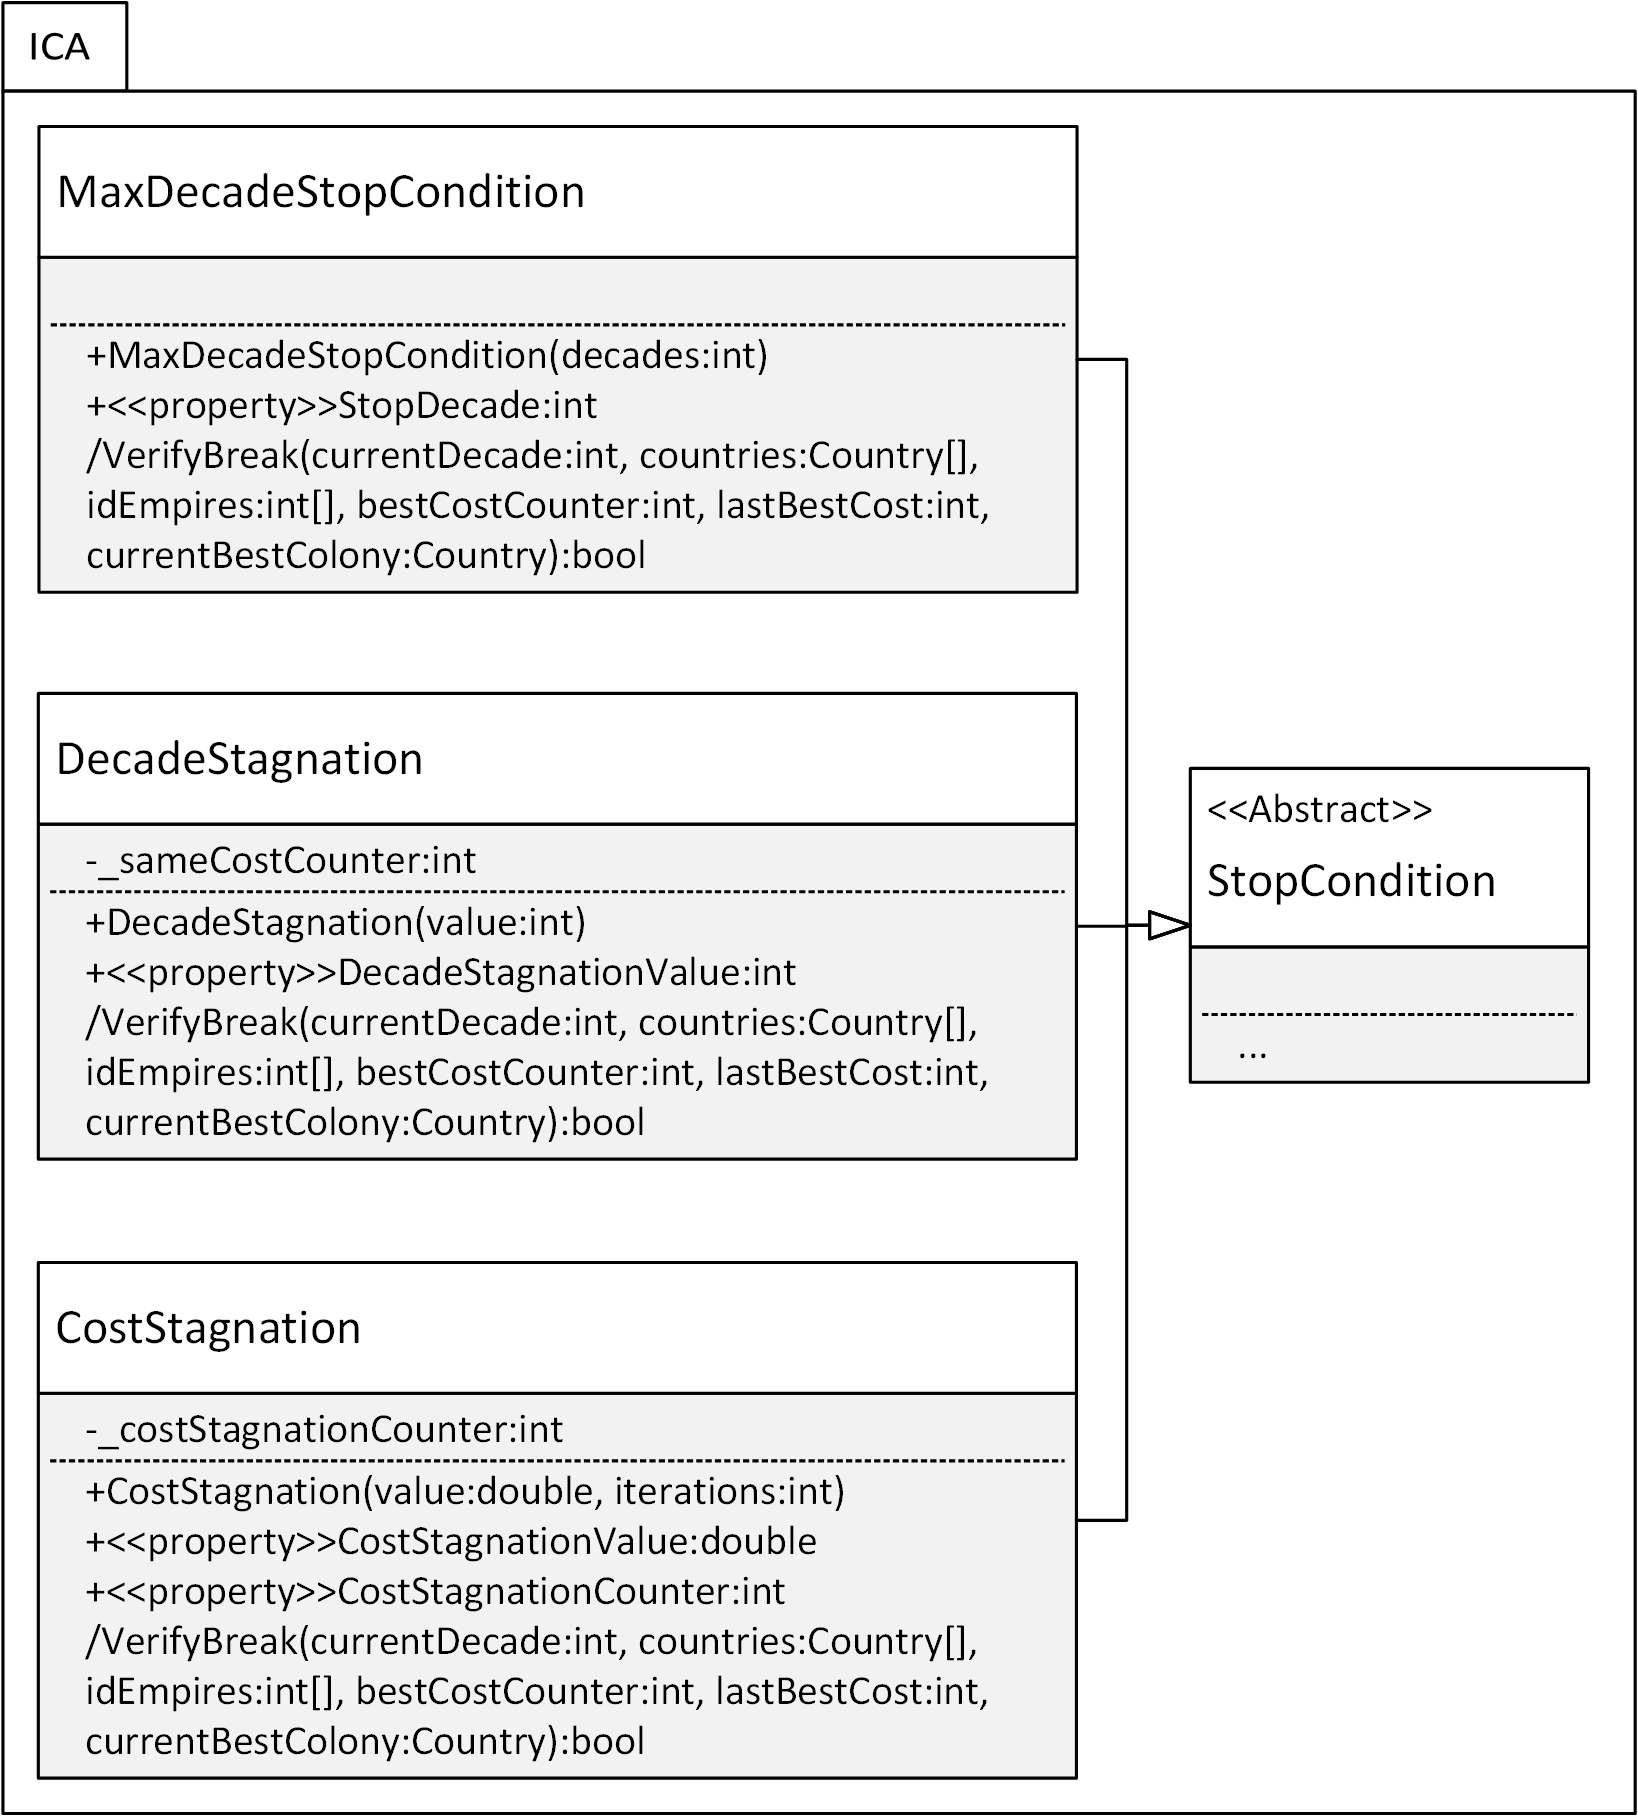
\includegraphics[scale=1]{Figuras/ClassesICA-StopConditionsImplements.png}
	\caption{Implementação das condições de parada}
	\label{fig:ClassesICA-StopConditionsImplements}
	\end{figure}

Por fim, a classe \emph{ImperialistCompetition} controla toda a competição imperialista, desde a inicialização dos países até o término da competição. Ela é a implementação do fluxograma do ICA apresentado na metodologia, com alterações para adição de novos recursos como processamento paralelo e orientação a objetos, tornando o ICA genérico a qualquer problema. Sendo assim, todos os elementos, lógicas, condições e ideias descritas anteriormente no fluxograma são abstraídas de modo que esta classe processe a competição imperialista idealizada, usando de seus métodos e propriedades em conjunto com os demais elementos modelados (classe \emph{Country}, classe abstrata \emph{StopCondition} e interface \emph{IFitness}).

A Figura \ref{fig:ClassesICA-ImperialistCompetition} representa apenas a classe em questão, destacando em tom mais claros, na área onde se situam os membros da classe, elementos que fazem alguma ligação de relacionamento, seja esta uma associação, agregação ou composição, que podem ser melhor visualizados na Figura \ref{fig:ClassesICA-ICAResumed}, que por sua vez representa toda a implementação do ICA orientado a objetos e como os elementos se interagem, porém omite as propriedades e métodos das classes para que melhor visualização. Nota-se também na imagem que descreve a classe \emph{ImperialistCompetition} com suas propriedades e métodos, que para facilitar o entendimento foram adicionados comentários (texto entre \emph{'/*'} e \emph{'*/'}) que regionalizam as propriedades e métodos usados nesta classe, já que ela é a responsável por implementar, além dos conceitos básicos do ICA, todas as alterações estruturais e de otimização.

%Como a classe \emph{ImperialistCompetition} tem uma quantidade muito grande de propriedades e métodos, estes serão melhores detalhados no anexo, e neste texto, apenas serão detalhados os processos principais ao funcionamento da classe e como os elementos são usados para executar o processo evolutivo do ICA.

Uma das partes mais complexas do ICA é o preparo para o processo evolutivo, referindo-se a etapa de inicialização dos países presente no do fluxograma do ICA apresentado na metodologia pela Figura \ref{fig:Fluxograms-ICACanonic}, países estes, que por sua vez, devem estar separados em impérios antes que o este processo evolutivo de fato comece. Quando se instancia a classe \emph{ImperialistCompetition}, ainda não são efetuadas as tarefas responsáveis por esta etapa de inicialização dos países, pois ainda existirão valores que devem ser configurados, como a adição de um objeto do tipo \emph{IFitness} através da propriedade \emph{Fitness}, e definição dos limites do problema, sejam estes chamados pelo método \emph{InitializeBounds} ou adicionados manualmente nas propriedades \emph{MinBounds} e \emph{MaxBounds}.

A partir do momento em que todos os valores estão configurados apropriadamente, pode-se executar o método \emph{Run()}, que é dividido em duas etapas principais, onde uma delas consiste na etapa de inicialização dos países, e refere-se diretamente à primeira atividade presente no fluxograma do ICA apresentado na metodologia pela Figura \ref{fig:Fluxograms-ICACanonic}, e a segunda consiste no conjunto formado por todos os elementos presentes no \emph{loop} principal, definido como processo evolutivo, referentes ao restante das atividades presentes no fluxograma.


 \begin{figure}[h]
	\centering	
	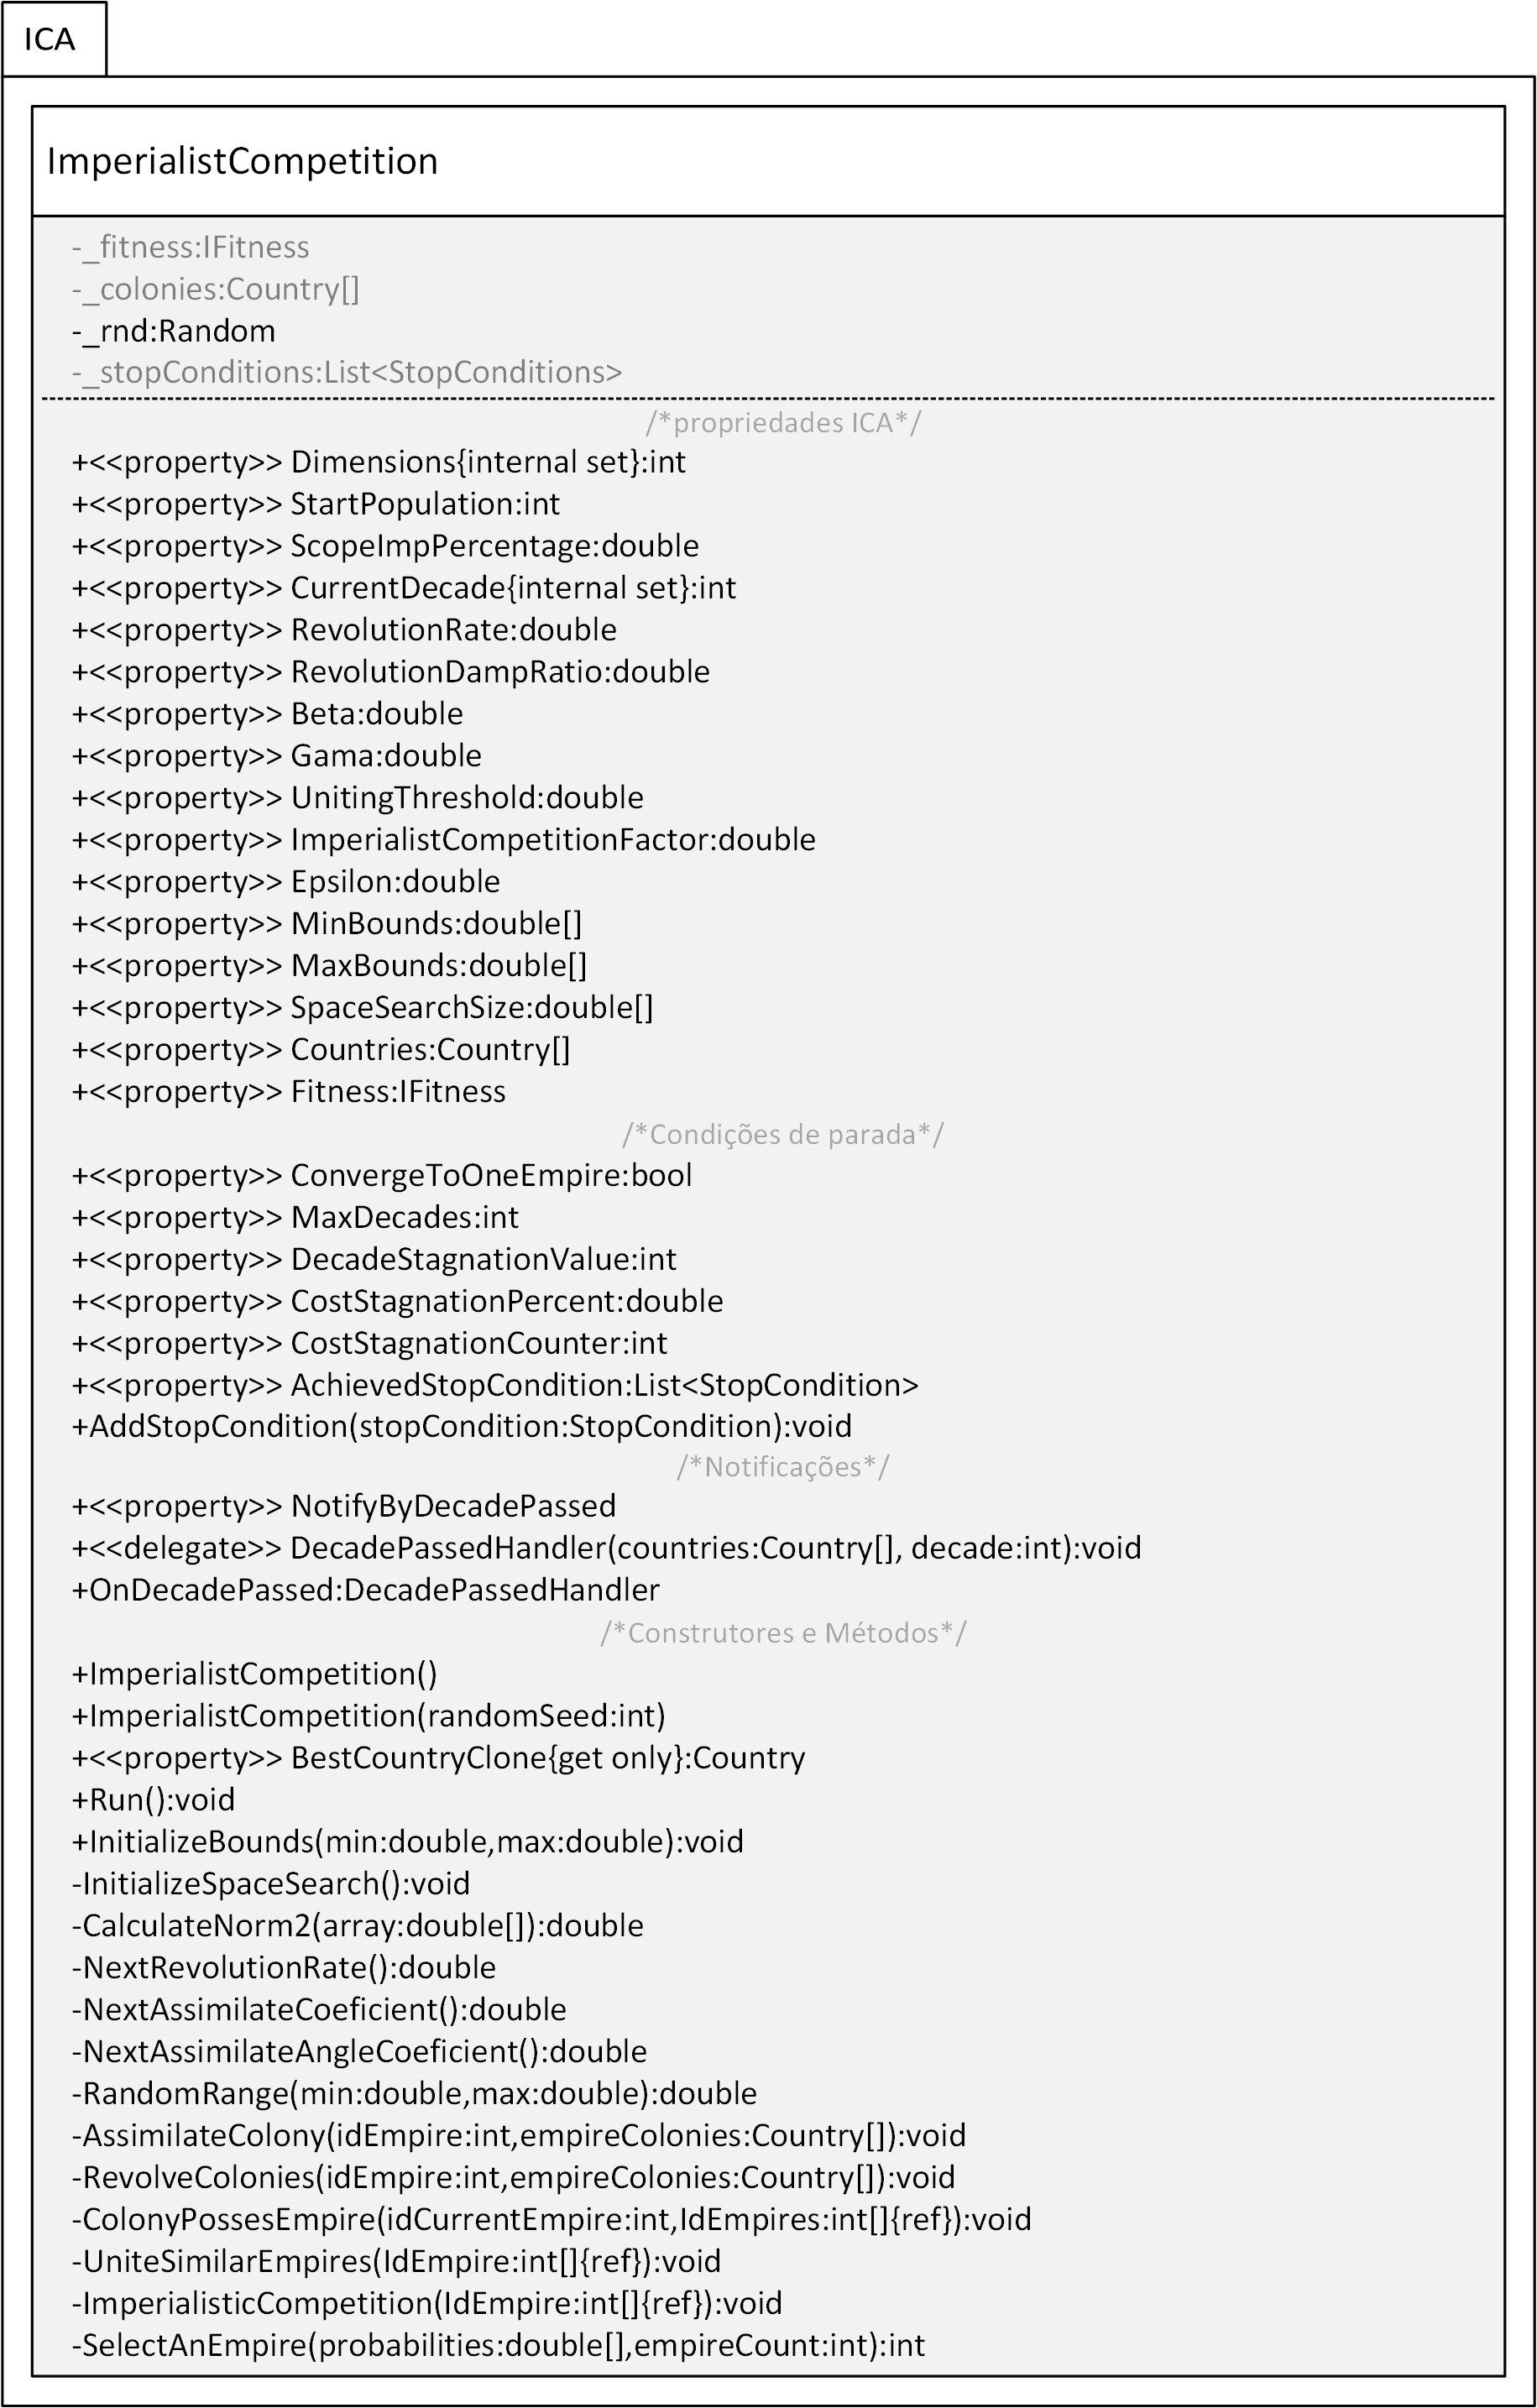
\includegraphics[scale=0.8]{Figuras/ClassesICA-ImperialistCompetition.png}
	\caption{Classe ImperialistCompetition}
	\label{fig:ClassesICA-ImperialistCompetition}
	\end{figure}
    
Então, assim que o método \emph{Run()} é chamado, inicia-se a etapa de inicialização dos países, que por sua vez tem como atividade inicial, instanciar as condições de parada padrões, sendo elas:

\begin{itemize}
\item Condição de parada por número máximo de décadas; 
\item Condição de parada por estagnação de custo idêntico durante as décadas; 
\item Condição de parada por estagnação de custo em um intervalo durante as décadas, do ICA. 
\end{itemize}

Observe ainda, que o relacionamento apresentado na Figura \ref{fig:ClassesICA-ICAResumed} é de agregação para estas três condições de parada, pois é nesta classe que elas são criadas e mantidas, porém o ciclo de vida destes objetos podem se estender para além do deste objeto, uma vez que existe a propriedade \emph{AchievedStopCondition}, que expõe tais objetos publicamente de forma que estes possam ser referenciados fora desta classe, caso contrário, o relacionamento em questão deveria ser de composição.

\begin{figure}[h]
	\centering	
	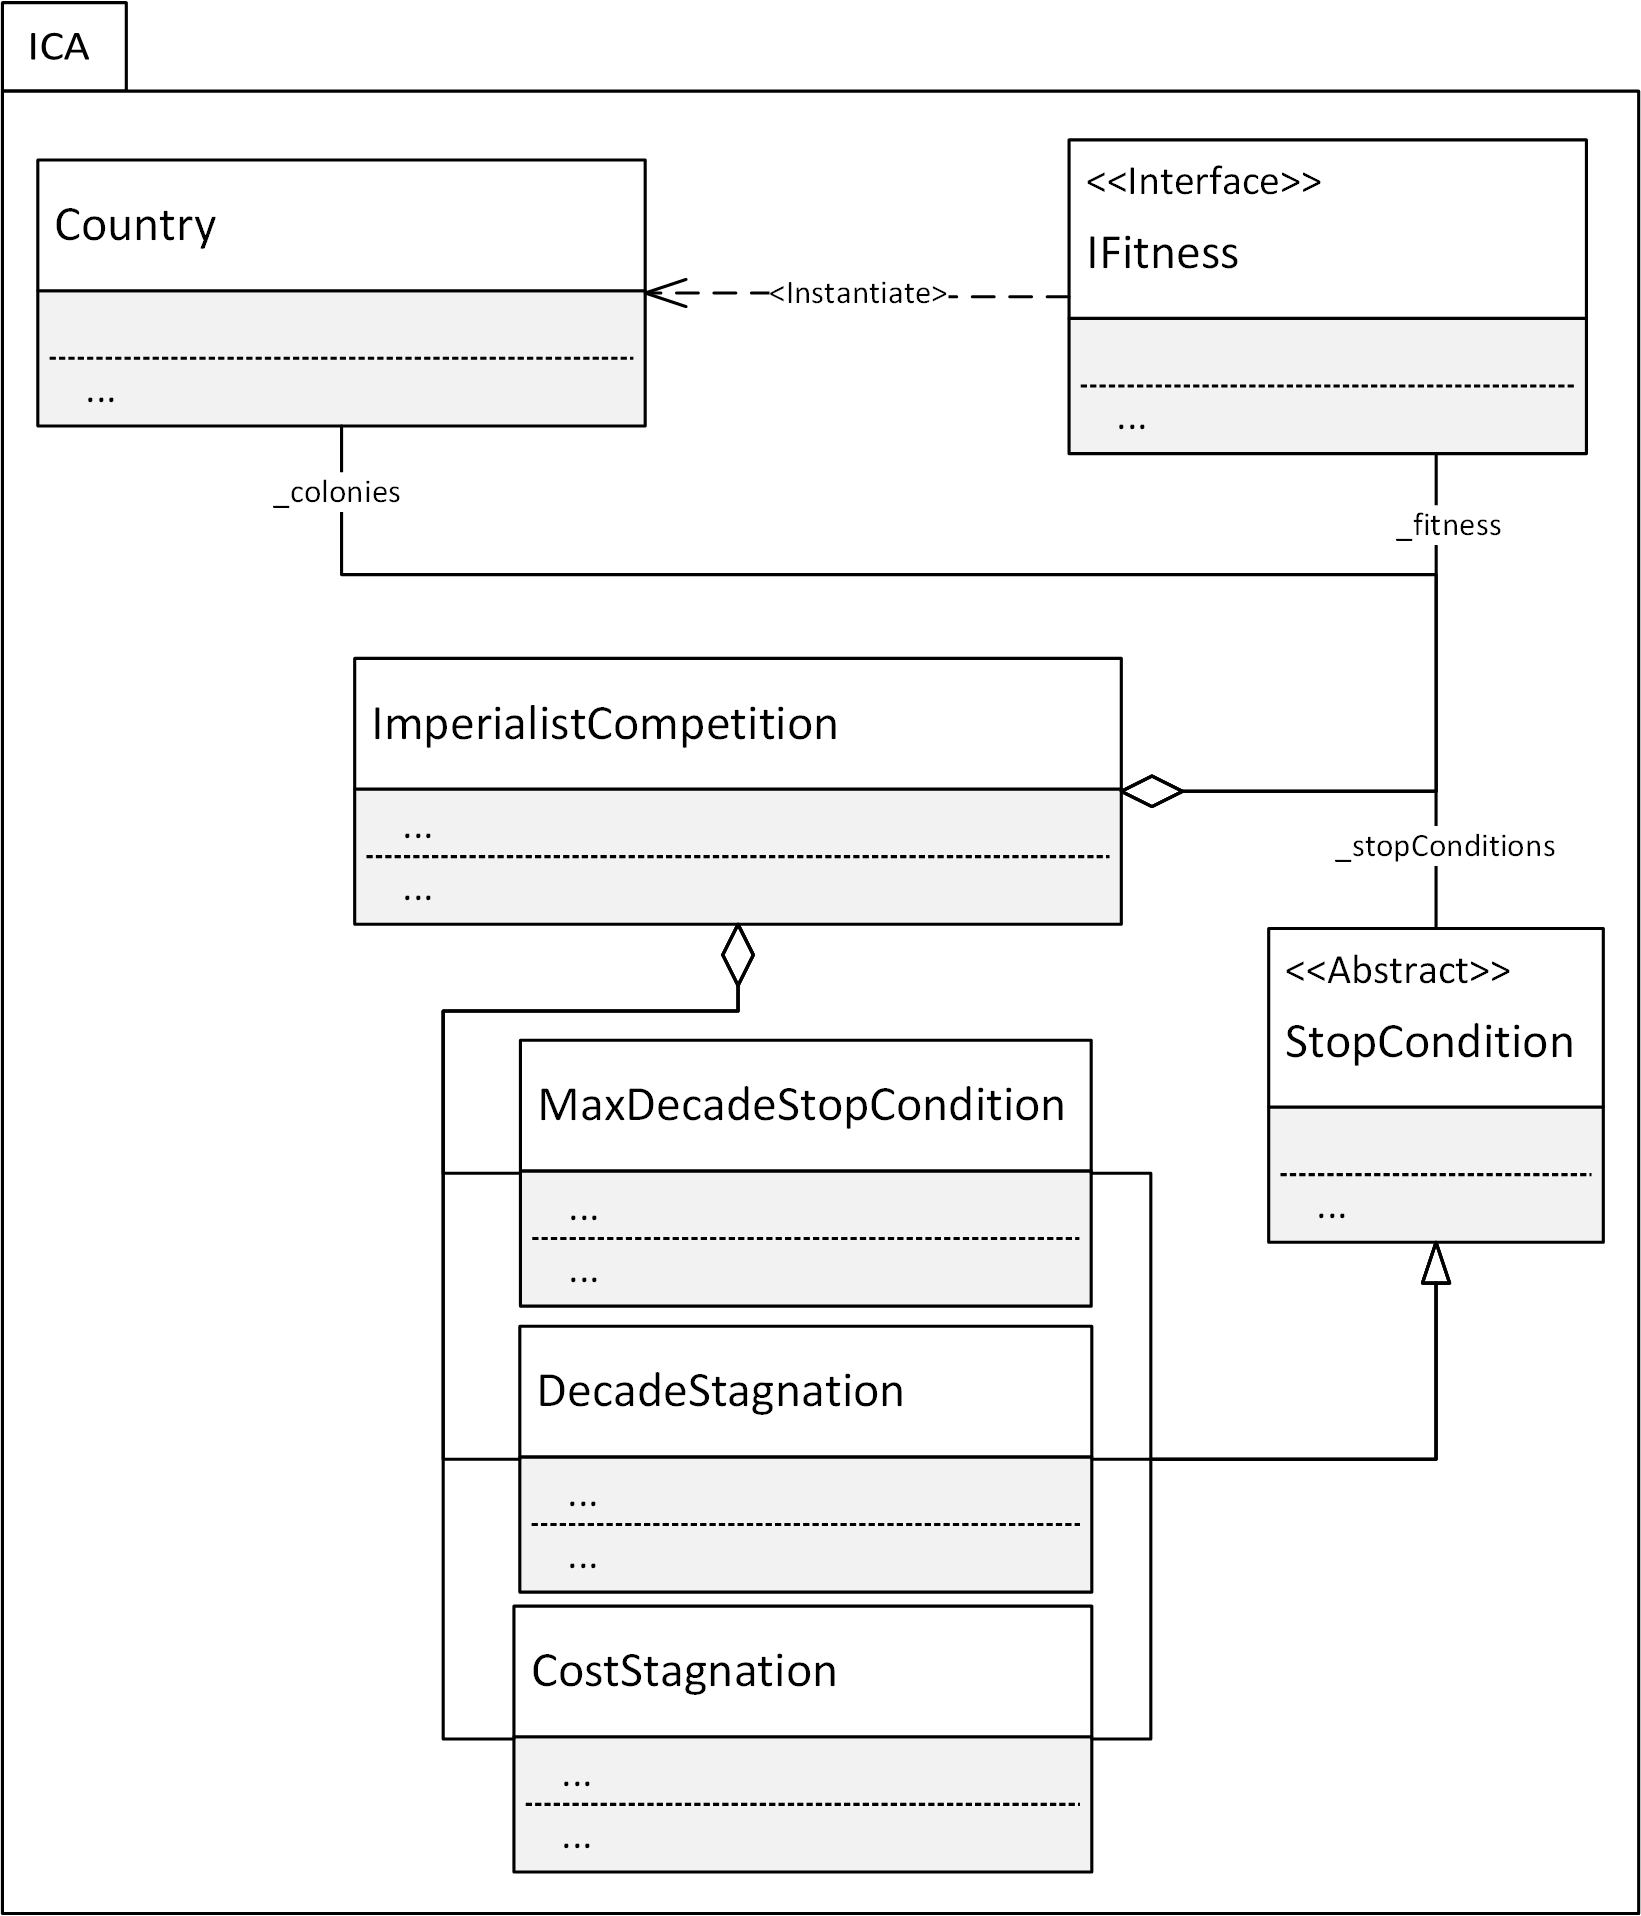
\includegraphics[scale=0.9]{Figuras/ClassesICA-ICAResumed.png}
	\caption{Diagrama de classes resumido do ICA }
	\label{fig:ClassesICA-ICAResumed}
	\end{figure}
    
Em seguida, inicializam-se os valores constantes ou de cálculo simples, como tamanho do espaço de busca (\emph{SpaceSearchSize}, pelo método \emph{InitializeSpaceSearch}), número populacional (\emph{nPop}), número de impérios (\emph{nImp}) e número de colônias (\emph{nCol}). Então, com estes valores já estipulados, faz-se uma chamada ao método \emph{GenerateCountries} do objeto \emph{Fitness} para que seja criado o vetor de países que será usado no processo evolutivo.

Mesmo tendo em mão este vetor com os países já inicializados para o problema em questão, não se pode dar a etapa de inicialização como terminada, pois ainda não foram gerados os impérios para que se comece a competição imperialista. Então, tão logo que se crie o vetor de países \emph{Countries}, deve-se fazer a chamada para a avaliação do custo de cada país contido nele. Neste caso, o processamento dos custos de cada país é feito pela chamada do método de avaliação \emph{Eval} do objeto \emph{Fitness} para cada país, que é feito de forma paralela, agilizando o processo de avaliação. Observe que deve-se tomar muito cuidado ao implementar o método de avaliação no objeto \emph{Fitness} para que este não compartilhe recursos globais (somente para escrita, pois a leitura de dados pode ser feita paralelamente), de forma que as diversas chamadas a este método de forma paralela não entrem em conflito, prendendo os recursos de processamento apenas para a tarefa em questão.

Com todos os custos calculados, deve-se definir agora, quais dos países serão os países imperialistas, porém, como foi decidido não criar classes extras apenas para separar imperialistas de colônias, foi criado um vetor de índices, que armazena quais os índices presentes no vetor de países \emph{Countries} representam os países imperialistas. Este vetor foi criado utilizando o recurso da linguagem C\# chamado LINQ, em apenas uma linha de código. Caso este recurso não existisse, seriam necessárias dezenas de linhas de código e chamadas de método para a criação deste vetor de índices. O processo para a criação deste vetor utilizando este recurso é relativamente simples, e envolve a seleção dos índices do vetor de países, ordenado-os e pegando os \emph{nImp} primeiros valores.

Após a criação deste vetor de índices de países imperialistas, deve-se calcular o poder de cada império para que os países restantes sejam distribuídos como colônias dos países imperialistas formando assim os impérios, e para isto, cada país imperialista deve ter um número de colônias que seja proporcional ao seu poder. Para se obter tal valor, gera-se o vetor de valores inteiros \emph{nOfColonies} de tamanho \emph{nImp}, onde cada índice deste vetor representará a quantidade de colônias que cada império terá. 

Para se obter os valores do vetor \emph{nOfColonies} deve-se calcular o poder dos países imperialistas, multiplicá-lo pelo número de colônias \emph{nCol} e por fim arredonda-lo como proposto na equação. Para se obter o valor de poder \emph{pn} de cada país imperialista deve-se calcular inicialmente o custo normalizado para todos os países imperialistas e então atribuir como poder \emph{pn}, de um dado império \emph{n}, a divisão entre seu custo normalizado \emph{C.N.n} pela soma te todos os custos normalizados como demonstrado na metodologia. 

Originalmente o resultado do número de colônias é o arredondamento da multiplicação entre o poder \emph{pn} calculado e o número de colônias \emph{nCol}, porém computacionalmente existe o problema que arredondamentos na computação na verdade são truncamentos, por este ser um ambiente discreto e não contínuo, então é necessária uma etapa extra para verificar se o número total de colônias está correto, e caso não esteja, corrige-se o valor até que a soma dos valores do vetor \emph{nOfColonies} seja igual ao \emph{nCol}, adicionando-se 1 e incrementando o índice do vetor, como pode ser visto na primeira atividade condicional do fluxograma presente na Figura \ref{fig:Fluxograms-RunMethodStart}.

 \begin{figure}[h]
	\centering	
	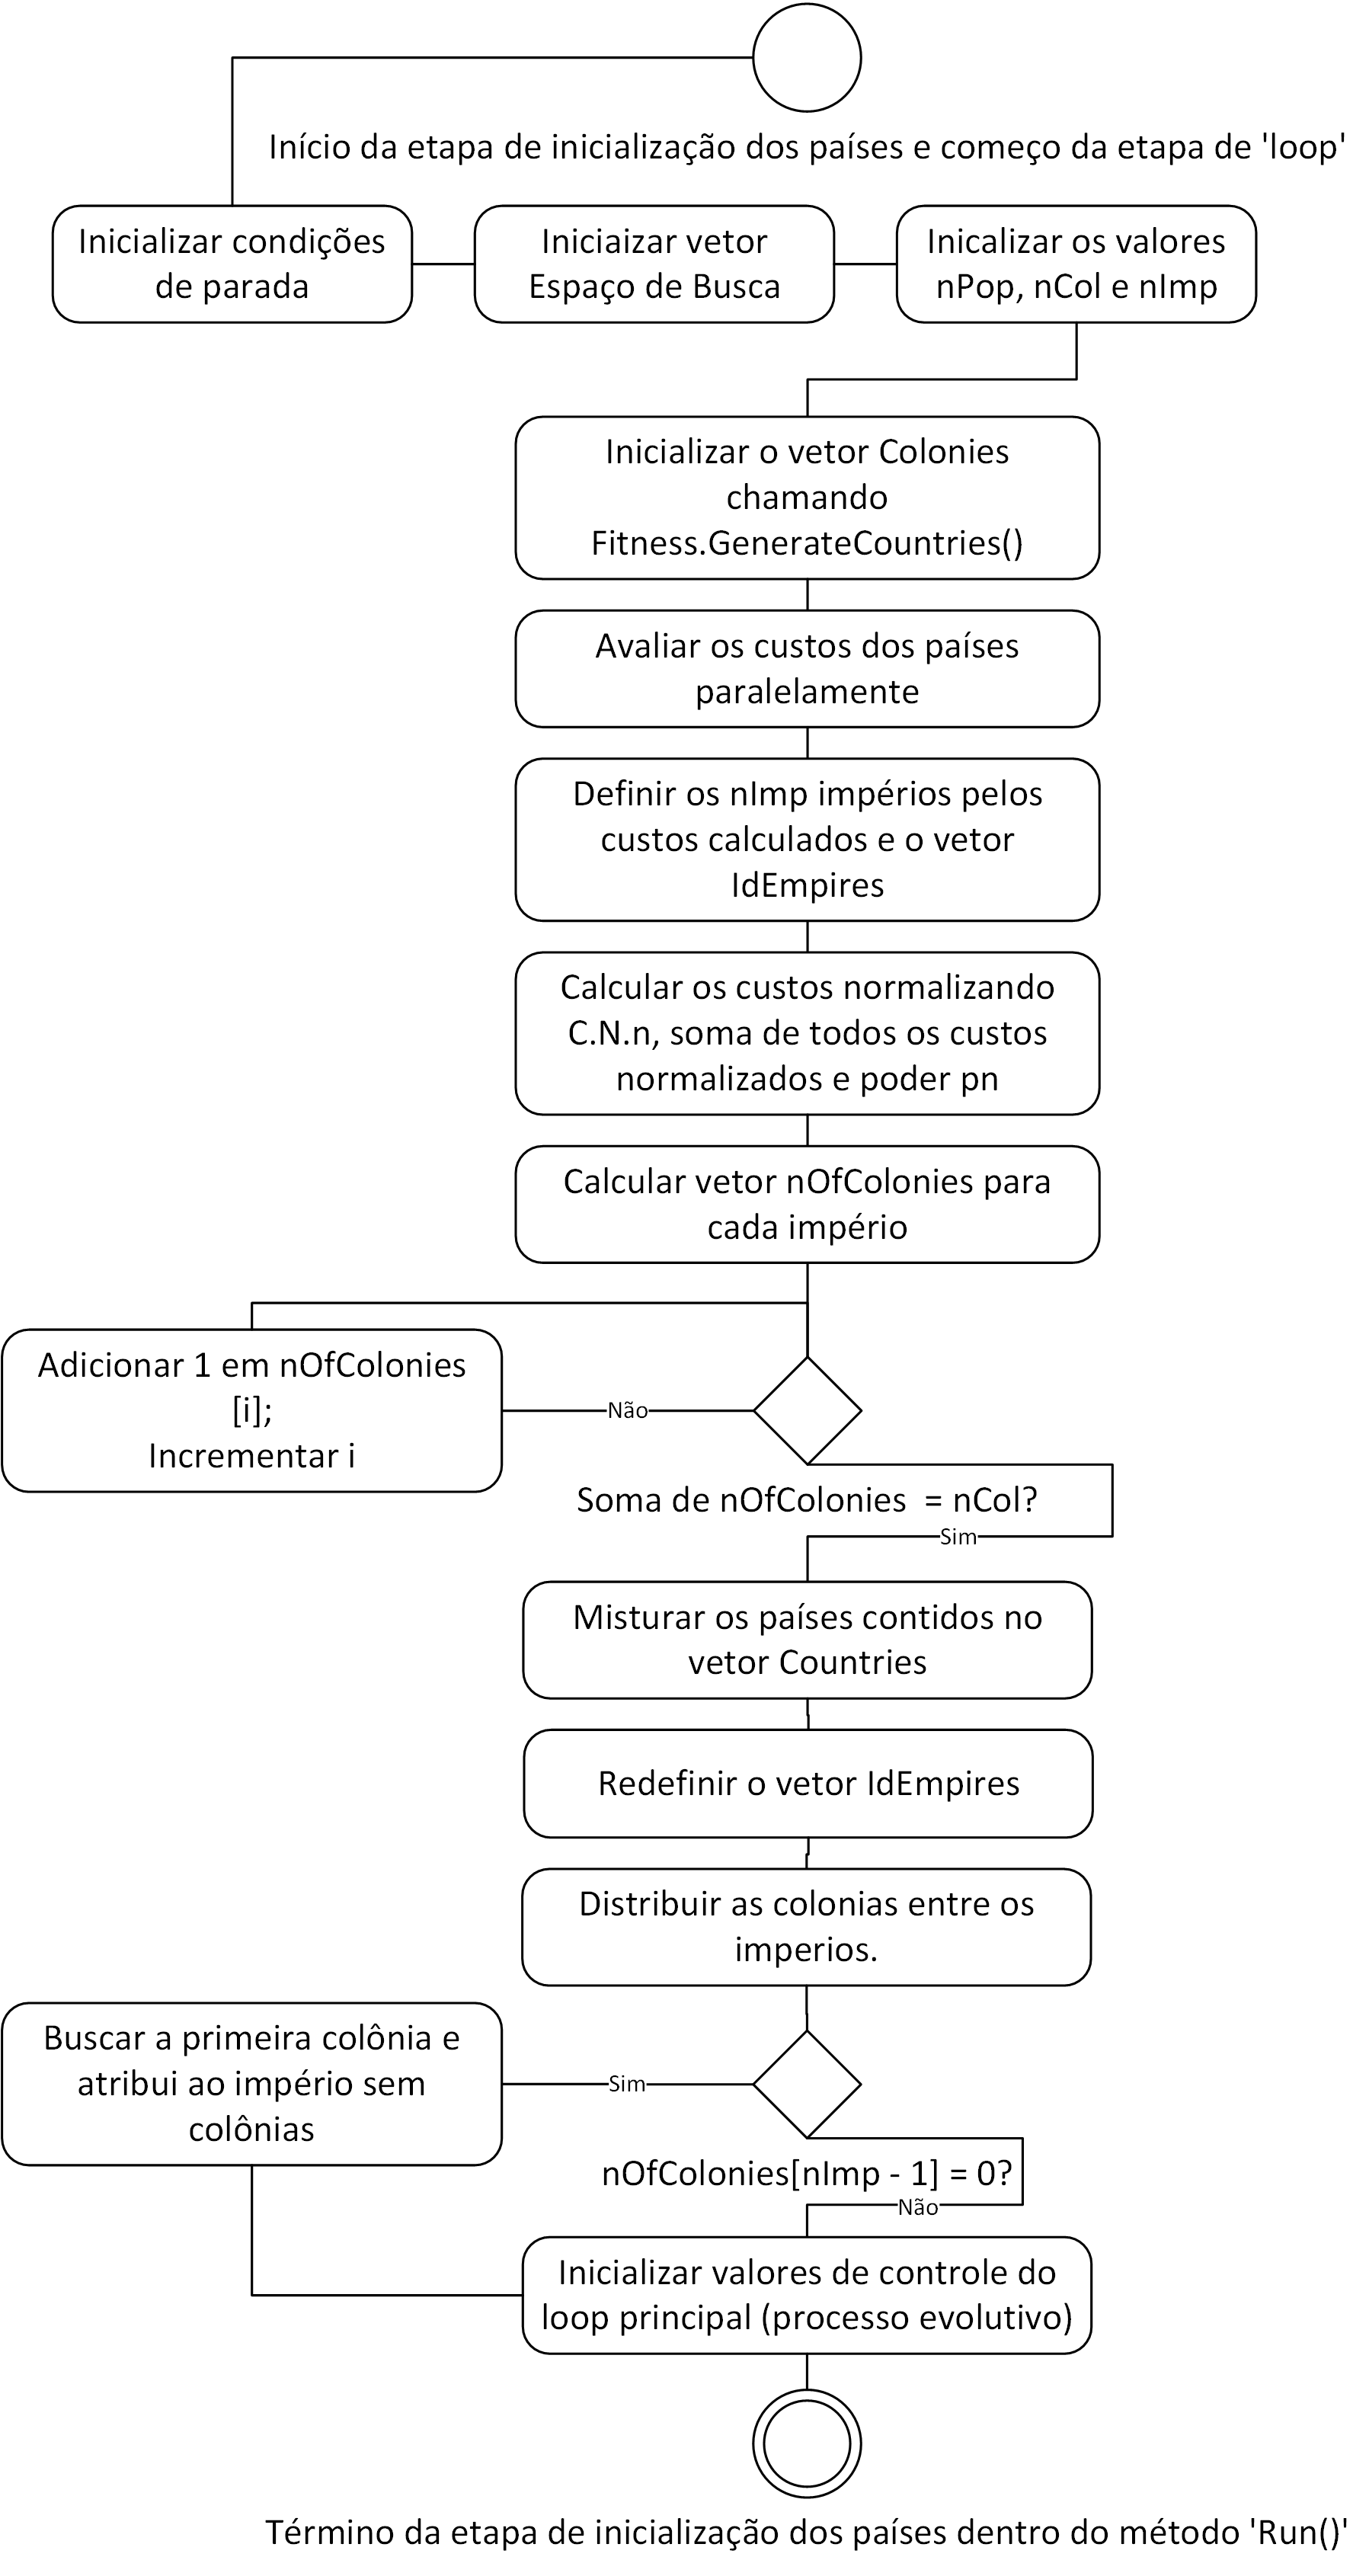
\includegraphics[scale=0.7]{Figuras/Fluxograms-RunMethodStart.png}
	\caption{Fluxograma da etapa de inicialização no método Run}
	\label{fig:Fluxograms-RunMethodStart}
	\end{figure}
    
Antes que se distribua as colônias para os impérios, o vetor contendo os países deve ser misturado, pois as colônias devem ser aleatoriamente distribuídas entre os impérios. Quando se efetua esta mistura, o vetor \emph{IdEmpires} deve ser redefinido para que se atualize os novos índices dos países imperialistas, pois o vetor de países \emph{Countries} sempre conterá os países imperialistas e suas colônias, e também nunca terá sua quantidade alterada. O ICA é um algoritmo que não destrói ou constrói países durante seu processo evolutivo, ele apenas altera seus atributos. 

A distribuição das colônias para os impérios ocorre iterando-se em \emph{i} inicialmente pelo vetor de impérios \emph{IdEmpire} uma única vez, e a cada iteração de \emph{i}, itera-se em \emph{j}, \emph{nOfColonies[i]}, efetuando assim a relação império (pelo vetor \emph{IdEmpire}) por número de colônias (pelo vetor \emph{nOfColonies}). Agora basta ir iterando o valor \emph{nCountry} sempre que se atribuir uma colônia a um império. Esta atividade que distribui as colônias entre os impérios pode ser melhor visualizada pelo fluxograma apresentado na Figura \ref{fig:Fluxograms-RunMethodEmpireDistribution}.

 \begin{figure}[h]
	\centering	
	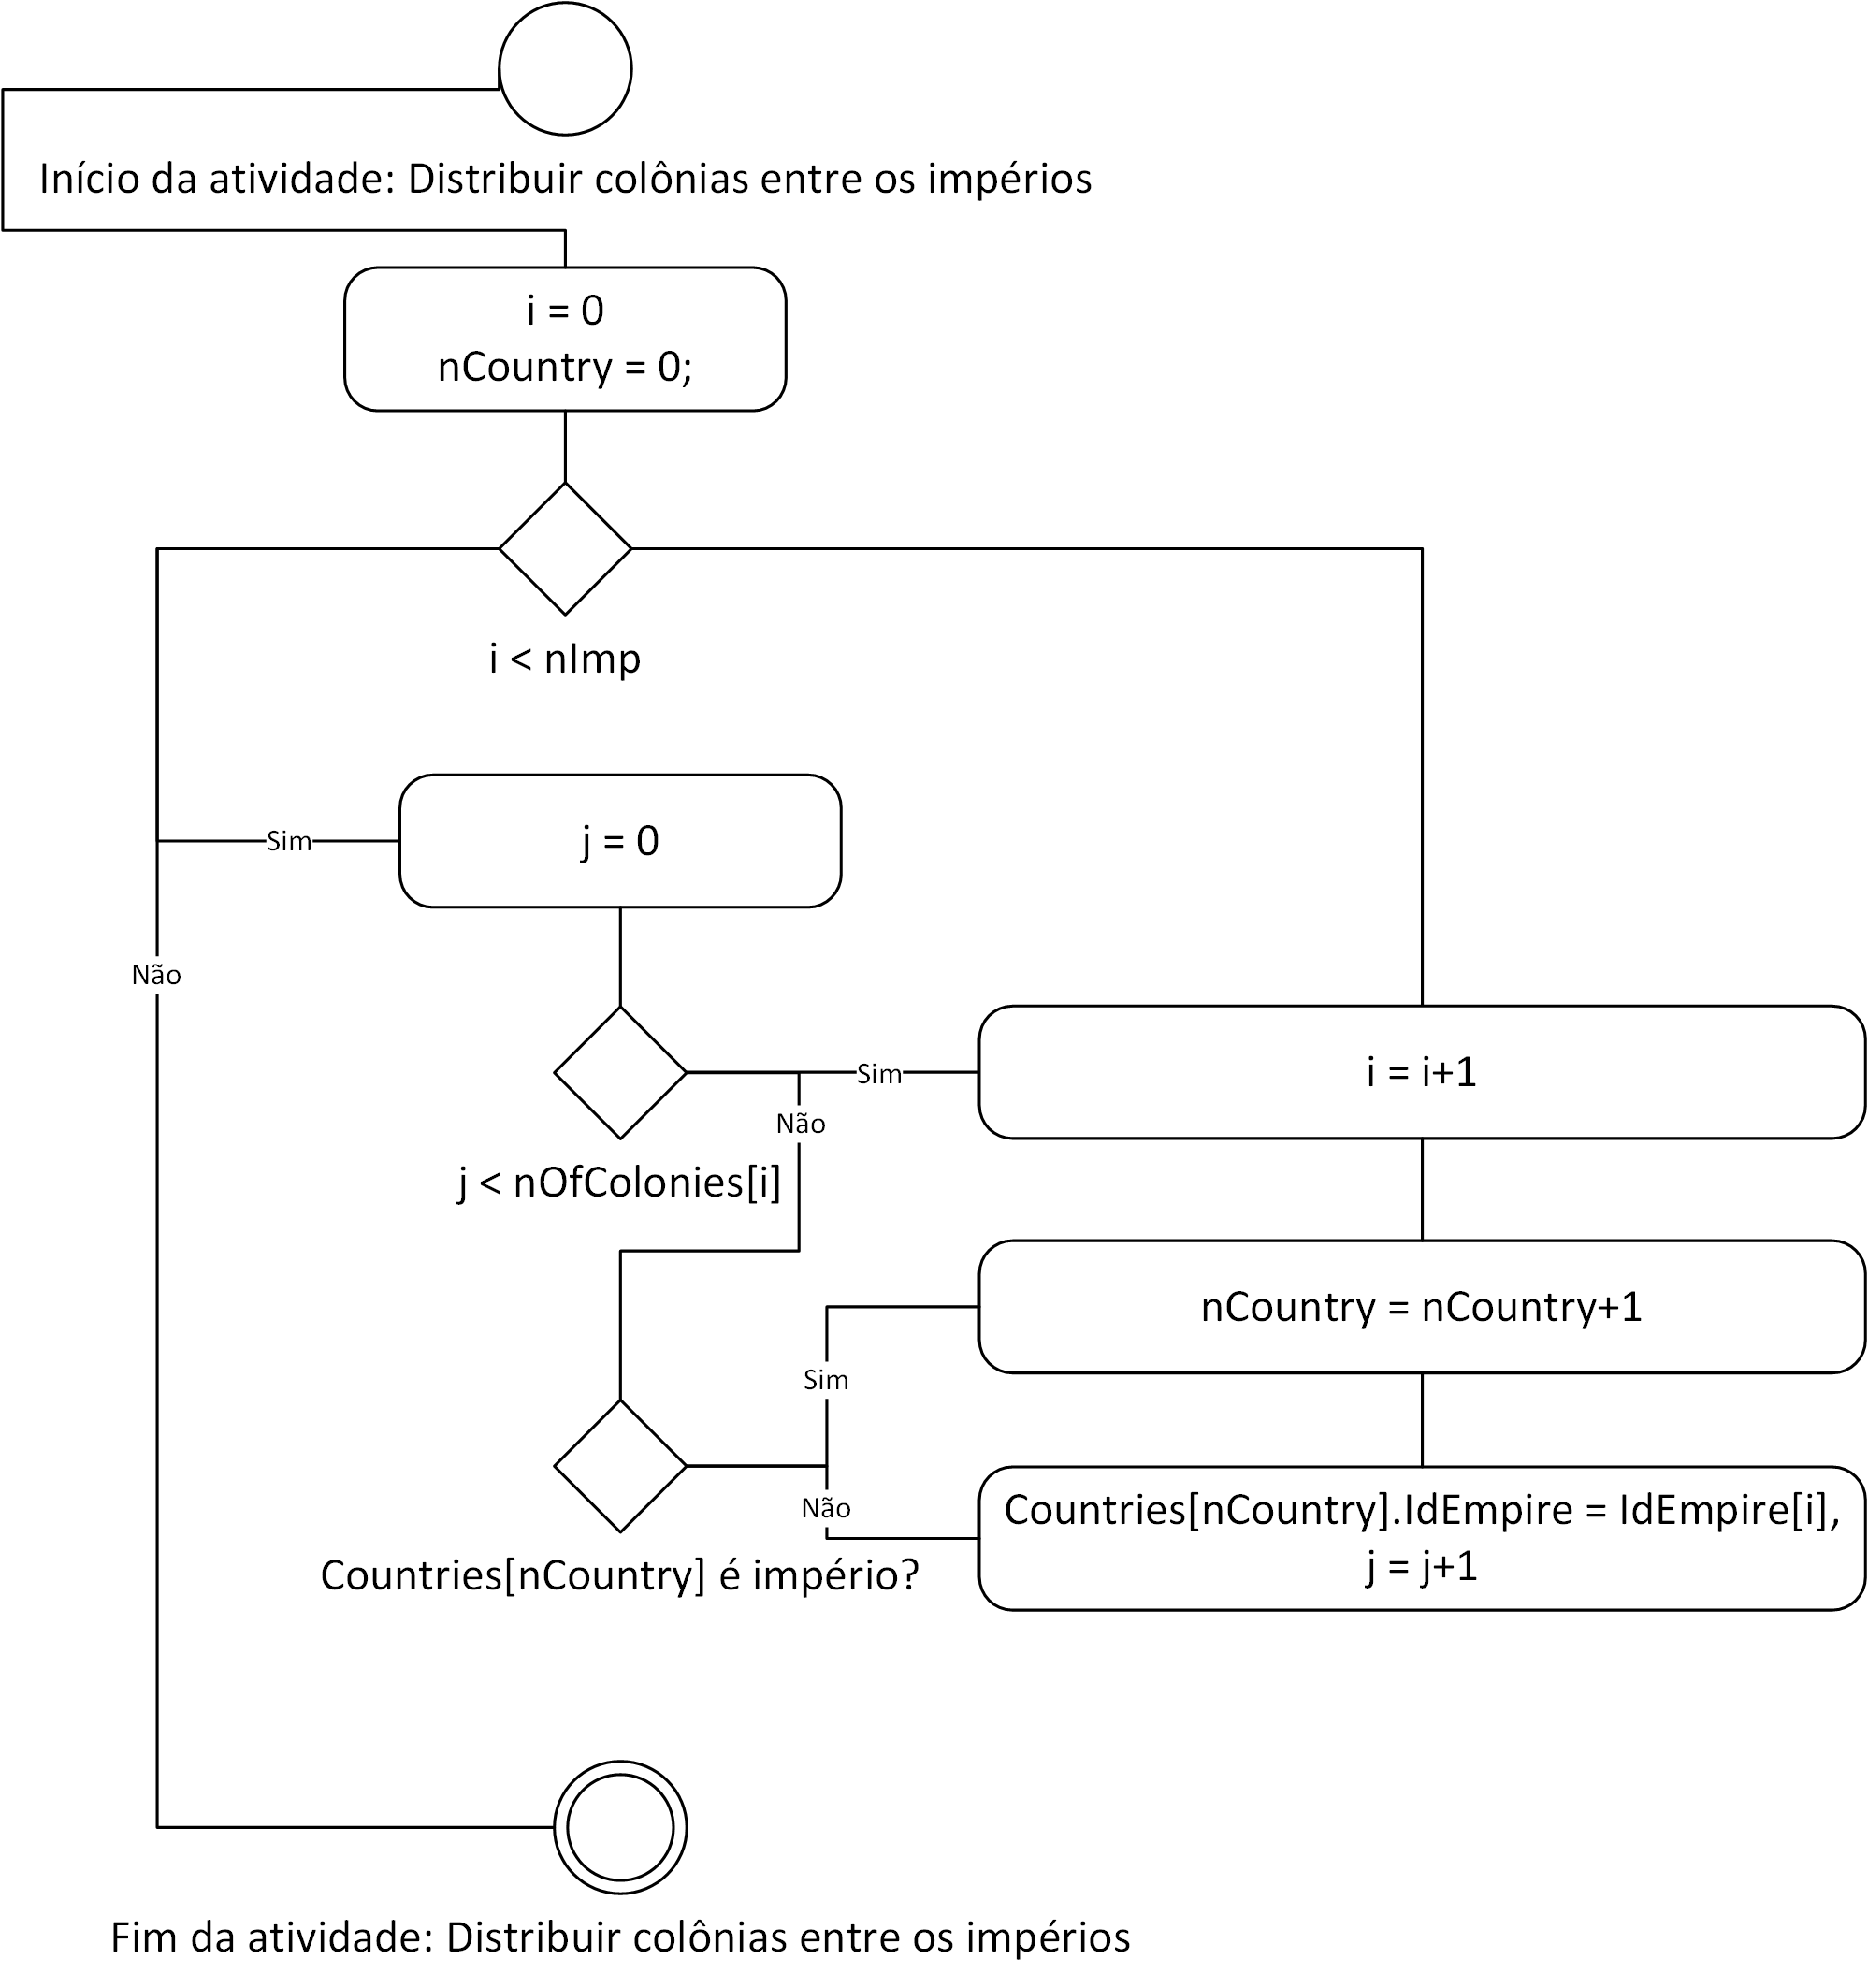
\includegraphics[scale=0.7]{Figuras/Fluxograms-RunMethodEmpireDistribution.png}
	\caption{Fluxograma sobre a distribuição de colônias entre os impérios}
	\label{fig:Fluxograms-RunMethodEmpireDistribution}
	\end{figure}

Após a distribuição das colônias entre os impérios, ocorre uma verificação para certificar-se de que o último império tem pelo menos uma colônia, e caso ele não tenha, a ele é atribuída uma colônia arbitrária de um dos outros império. Note que esta etapa traz a impressão de ser semelhante a etapa que verifica se a soma do vetor \emph{nOfColonies} é igual a \emph{nCol}, porém são coisas distintas, pois a condição \emph{nOfColonies} == \emph{nCol} não implica que todos os impérios devam ter pelo menos 1 colônia. 

Com a etapa de inicialização dos países finalizada, agora existem impérios, os quais possuem colônias que foram atribuídas de forma proporcional e arbitrariamente, e estes impérios e suas colônias estão espalhados por todo espaço de busca aleatoriamente, prontos para iniciar o processo evolutivo do ICA. O processo evolutivo no ICA caracteriza-se por um processo iterativo (\emph{loop}) onde os elementos, que já estão dispostos no espaço de busca, começam a alterar seus atributos para encontrar a melhor solução presente neste espaço de busca. Então, durante o processo evolutivo ocorrem várias operações nas colônias  e impérios de forma a atingir a melhor solução, e consequentemente parar este processo iterativo. 

Observando novamente o fluxograma do ICA apresentado na metodologia pela Figura \ref{fig:Fluxograms-ICACanonic}, é possível notar as operações:
\begin{itemize}
\item Assimilação colonial - movimentação da colônia para o império,
\item Possessão imperial - colônia mais poderosa toma o império para si, e
\item Competição imperialista - a colônia mais fraca do império mais fraco é passada para o império mais propenso a tê-la.
\end{itemize}

A delimitação destes elementos pode ser observada na Figura \ref{fig:Fluxograms-ICACanocicDetailed}, assim como a separação entre a etapa de inicialização e o processo evolutivo. Estas operações são suficientes para encontrar soluções em qualquer espaço de busca, porém, este trabalho apresenta algumas adições de operações  ou melhoras de alguns métodos, a fim de otimizar tanto o tempo de convergência quanto a precisão da busca pela melhor solução, e ainda, de modo que estas operações ocorram de forma agregada ao fluxo anterior. Estas alterações são mencionadas nas subseções seguintes, e aqui nesta seção serão apresentados apenas alguns detalhes referentes ao funcionamento de tais alterações. 

A primeira etapa, logo após a entrada no \emph{loop} principal é a de notificação, que envia para todos os elementos registrados nesta classe uma cópia do vetor de países \emph{Countries} e o valor da década atual \emph{CurrentDecade}. Assim, qualquer objeto que esteja "ouvindo" pode fazer o rastreio de todos os países e impérios durante as décadas.

 \begin{figure}[h]
	\centering	
	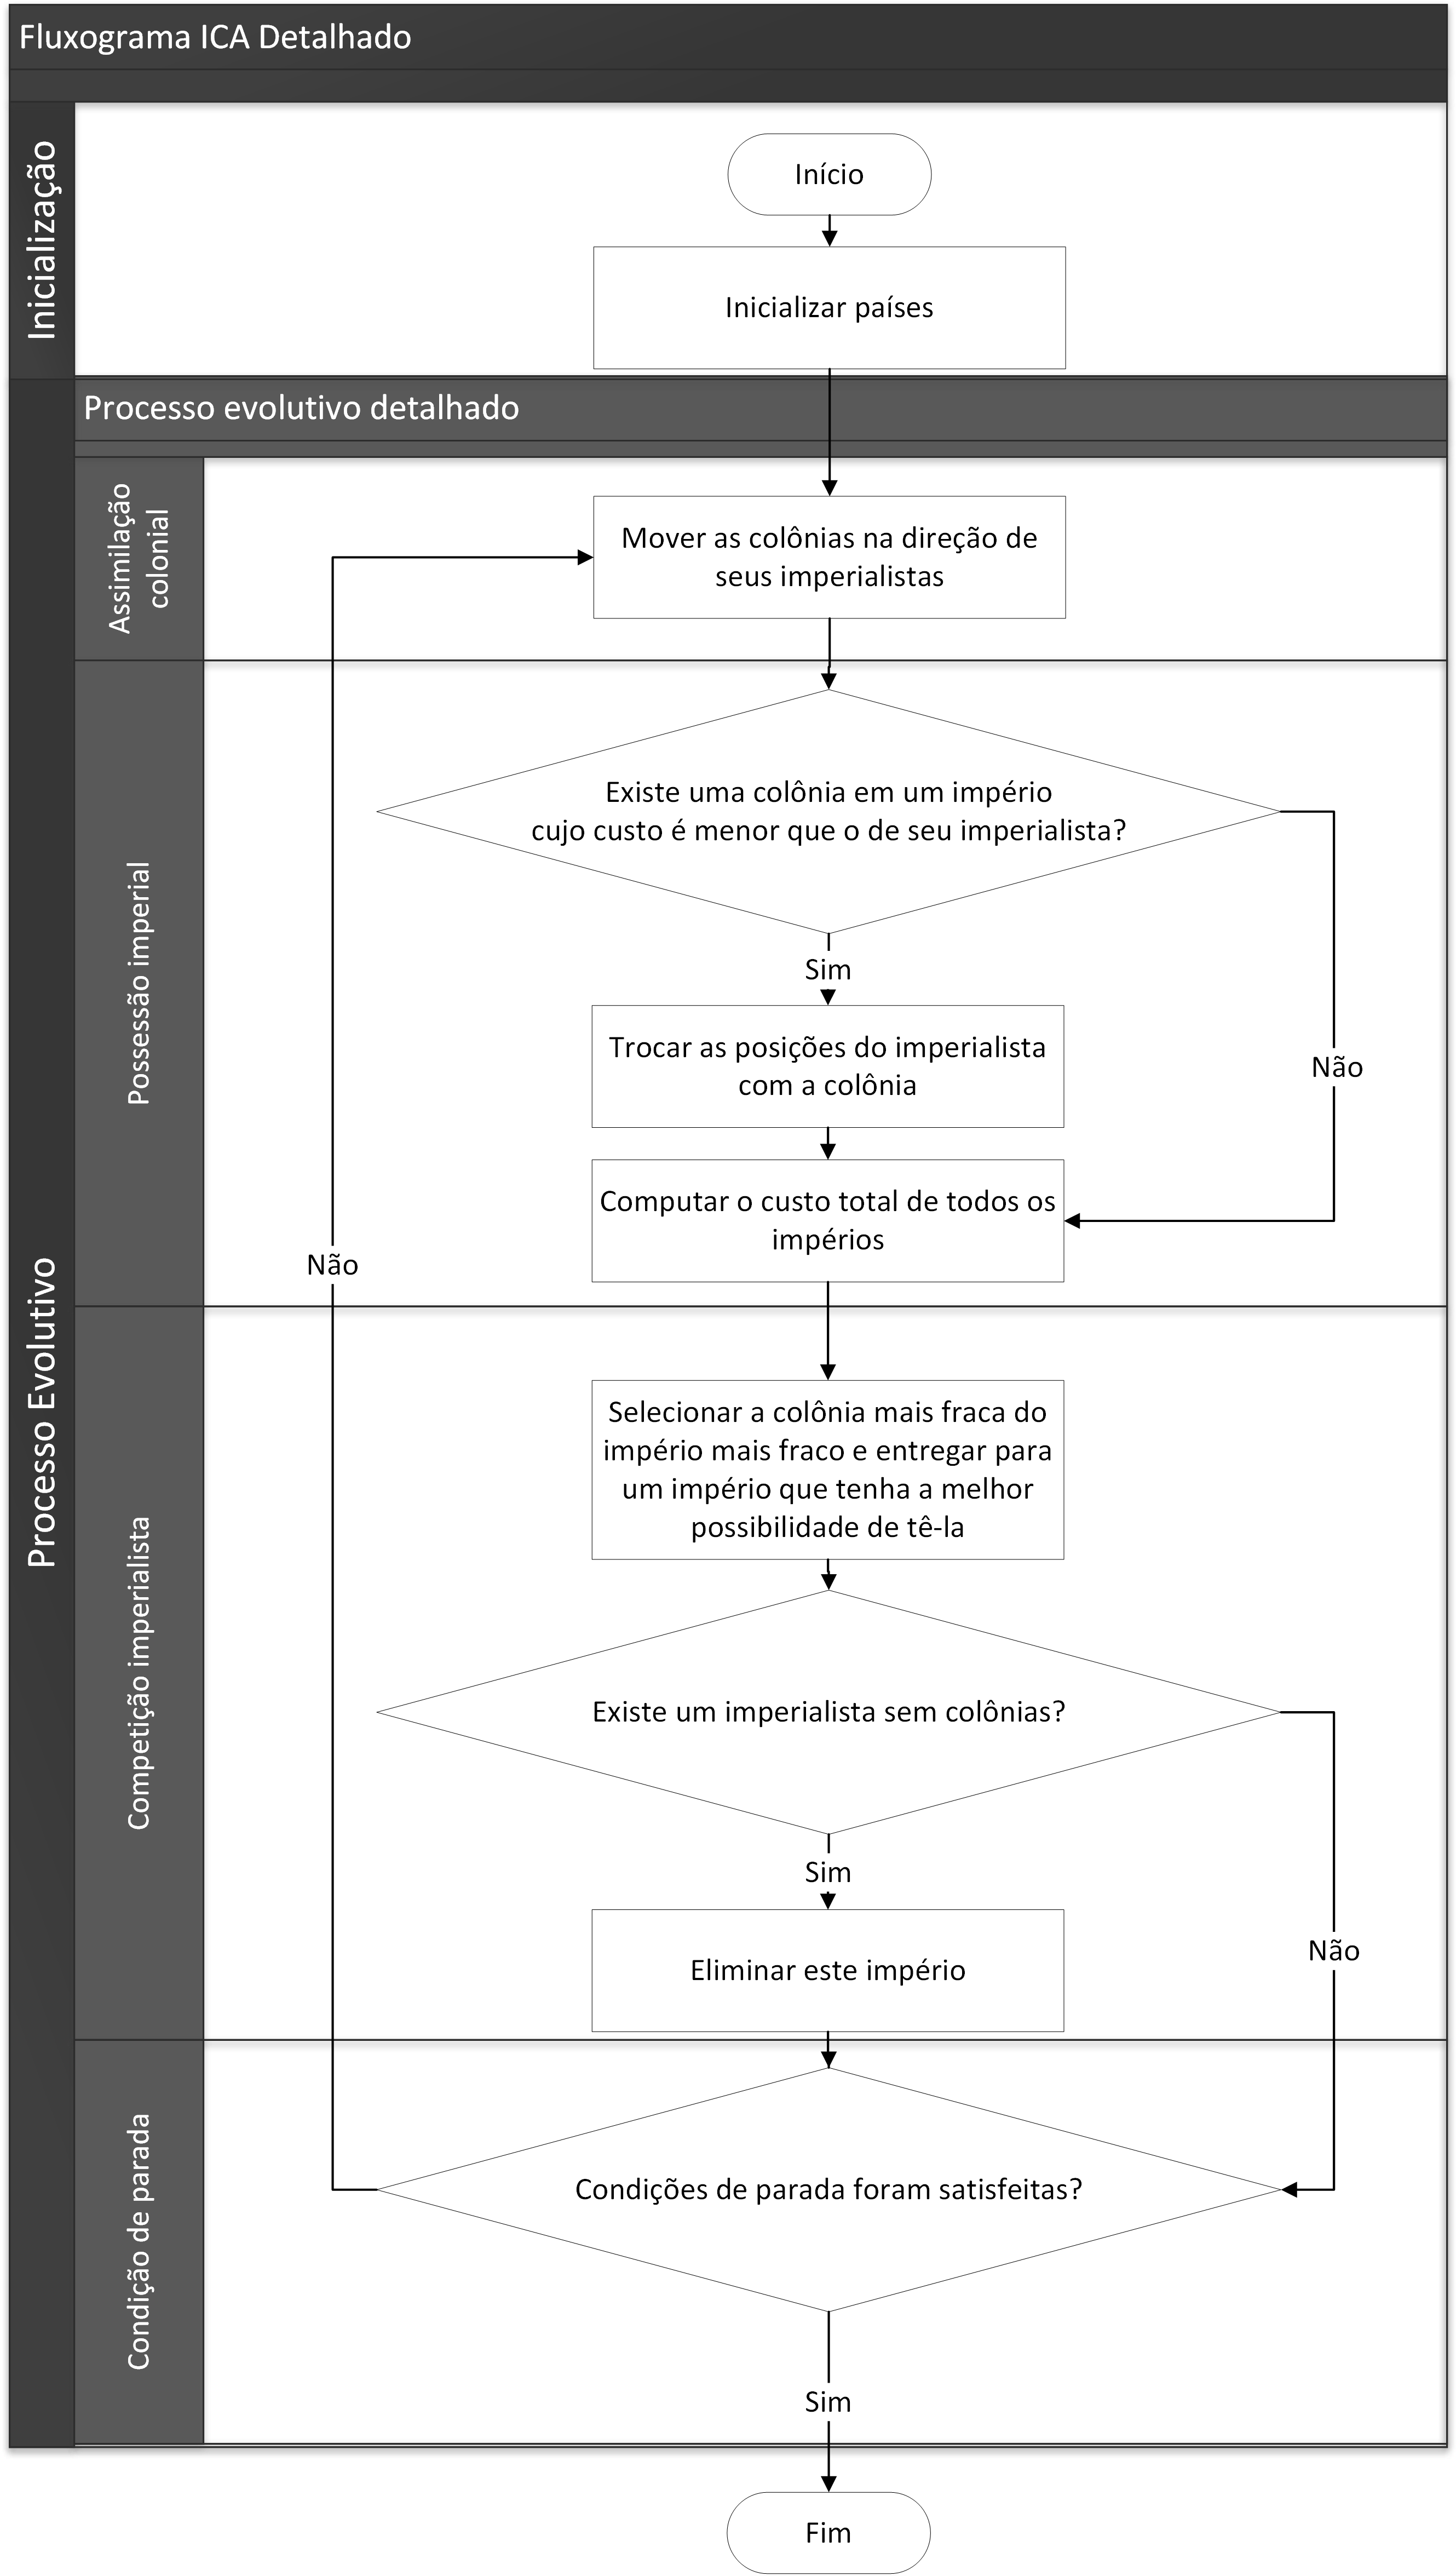
\includegraphics[scale=0.5]{Figuras/Fluxograms-ICACanocicDetailed.png}
	\caption{Fluxograma ICA detalhado}
	\label{fig:Fluxograms-ICACanocicDetailed}
	\end{figure}
	
Foram efetuadas algumas alterações na ordem de algumas etapas, mas sem alterar o funcionamento do ICA. Assim, para esta próxima etapa foi inserido o bloco responsável por fazer a verificação das condições de parada, que antes de fazer uma verificação pela lista que contém todas estas condições de parada, passa por uma pré verificação, que não é uma condição de parada, que verifica se o ICA deve convergir para apenas um império (se o número de impérios é 1). Tal lógica de entrada para verificação das condições de parada pode ser vista no diagrama da Figura \ref{fig:Fluxograms-StopConditions}.

 \begin{figure}[h]
	\centering	
	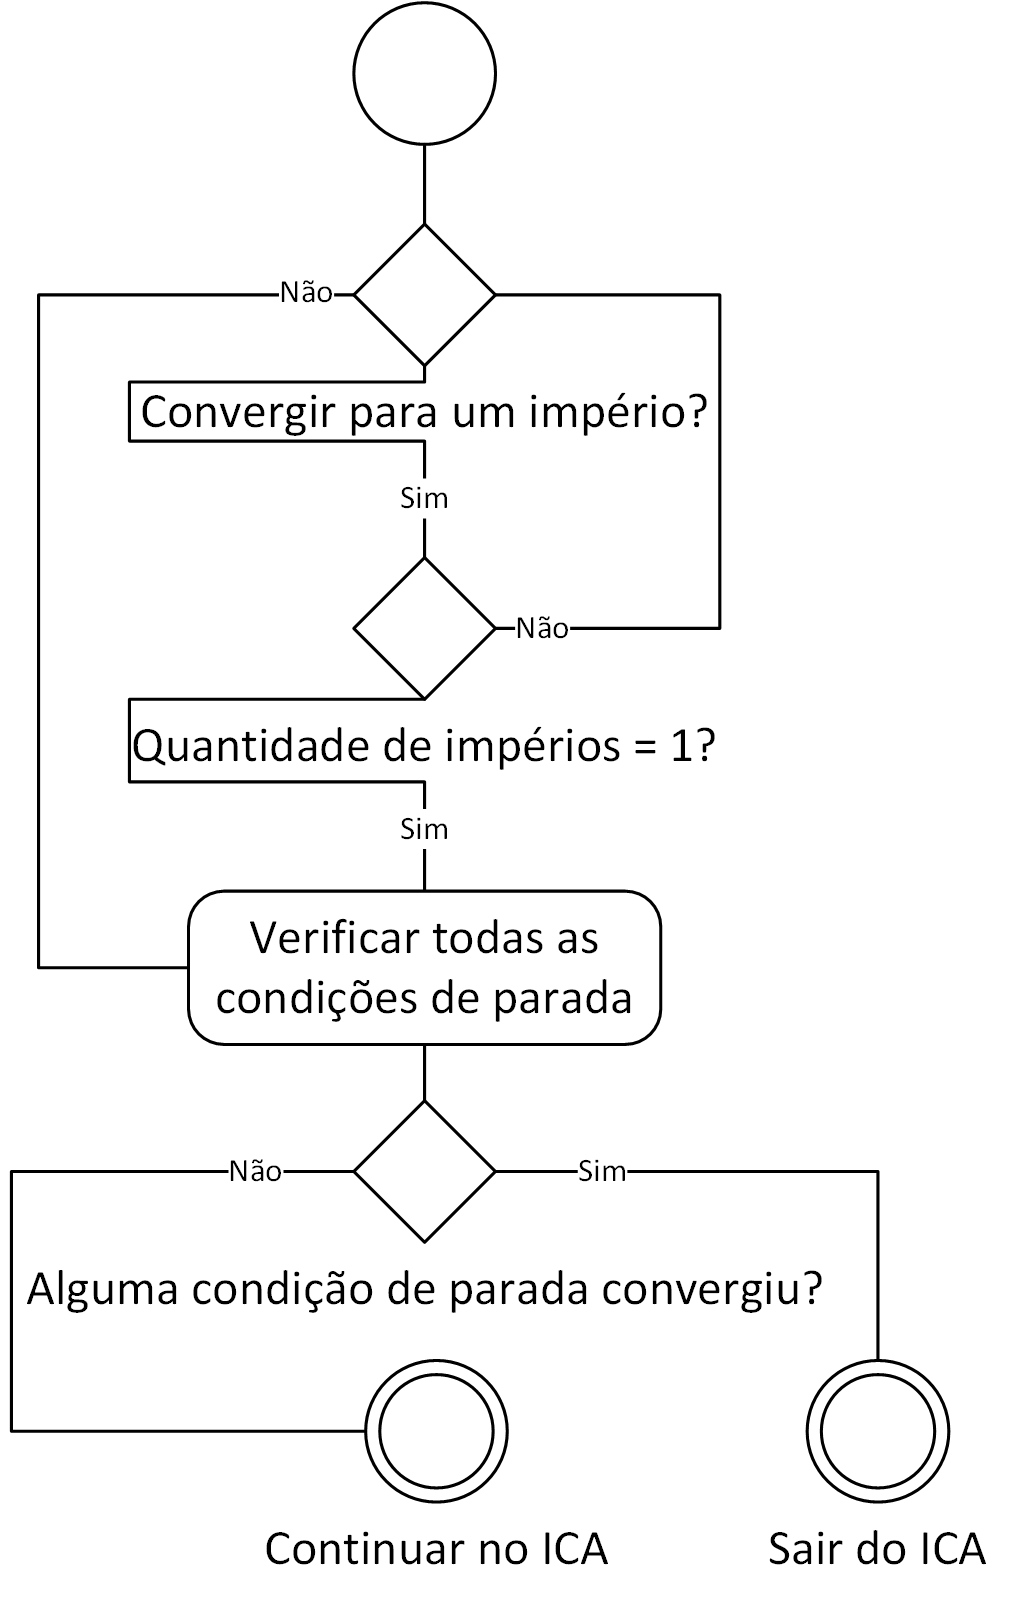
\includegraphics[scale=0.7]{Figuras/Fluxograms-StopConditions.png}
	\caption{Fluxograma sobre as condições de parada}
	\label{fig:Fluxograms-StopConditions}
	\end{figure}

Logo após a verificação das condições de parada, atualiza-se o valor da taxa de revolução, e em seguida efetua uma iteração por todos os impérios, fazendo a chamada para duas operações, sendo a primeira, a operação de assimilação colonial, que move as colônias em direção ao seu país imperialista, e a segunda, a nova operação de revolução, que por sua vez gera novos valores completamente aleatórios para o vetor de atributos de um dado país baseando-se em uma chance de ocorrência relativa a taxa de revolução mencionada anteriormente. Ambas operações são implementadas em métodos que recebem como parâmetro o valor do índice do império no vetor de colônias e uma lista de países contendo apenas as colônias pertencentes a este império.

Assim que a chamada destas duas operações ocorrer para todos os impérios, sabe-se que todas as colônias efetuaram a movimentação em direção ao seu imperialista e que uma porcentagem destas colônias pode ter passado pelo processo de revolução. Como os atributos destes países são alterados, é essencial que se recalcule os custos de todos os países, atualizando-os para que sejam utilizados nas demais operações do ICA. Nota-se também que apenas estas duas operações são as responsáveis por alterar os atributos dos países, assim, além de essencial, é imprescindível que a atualização dos custos ocorra.

O cálculo dos custos é feito pela chamada do método Eval pertencente ao objeto \emph{Fitness}, que por sua vez é o responsável por avaliar um dado país segundo o problema modelado pelo objeto em questão que implementa os métodos da interface \emph{IFitness}. A avaliação dos países é efetuada de modo paralelo não obstrutivo, ou seja, a avaliação de um dado país não depende dos demais países (Observa-se que a não obstrução no escopo do ICA é garantida, porém quando se implementa a interface \emph{IFitness} deve-se tomar cuidado para que o compartilhamento de recursos entre as tarefas não faça com que o processamento da avaliação de um país seja interrompido por outra, que requer o uso do mesmo recurso compartilhado). O fluxo do ICA só é continuado quando a avaliação de todos os países é finalizada, independente de se estar avaliando em paralelo ou série.

Seguindo o fluxo, a próxima operação verifica se existe uma colônia com poder maior que seu império, em caso positivo, esta colônia se torna o país imperialista, tomando para si as colônias do antigo império. São feitas diversas chamadas a esta operação, de forma iterativa, passando por todos os impérios, para que tal verificação possa ser efetuada através de um método que recebe como parâmetro o valor do índice do império no vetor de países \emph{Countries} e a referência do vetor que contém os índices de todos os impérios \emph{IdEmpires}.  


Esta operação executa, inicialmente, uma seleção no vetor \emph{Countries} a fim de filtrar todas as colônias do império em questão, em seguida, é necessário verificar se esta seleção resultou em um número de colônias igual a 0, o significa que este é um país imperialista sem colônias, e caso isto ocorra, para manter a consistência do ICA para as próximas operações, deve-se eliminar este império. Como mencionado anteriormente, um império quando é eliminado, têm seu país imperialista se tornando uma colônia do império mais forte, assim, esta operação segue os seguintes passos durante sua execução:
\begin{itemize}
\item Buscar pelo índice do melhor império e armazena localmente em \emph{bestEmpireId}.
\item Transforma o país imperialista sem colônias em uma colônia do país de índice \emph{bestEmpireId}.
\item Remove o índice do país imperialista que se tornara colônia, do vetor de índices de impérios \emph{IdEmpires} (sendo este o primeiro motivo de se passar a referência do vetor \emph{IdEmpires}, pois ele será atualizado). 
\end{itemize}

Caso a seleção das colônias seja maior que 0, significa que pode existir uma colônia cujo poder é maior que o de seu império, então se esta verificação for verdadeira, a colônia possuirá seu império, transformando o antigo país imperialista e suas colônias em colônias suas. Para efetuar esta troca executa-se a operação na sequência:

\begin{itemize}
\item Armazenam-se ambos os índices, da colônia que tomara o império e do país imperialista respectivamente em \emph{newEmpireId} e \emph{oldEmpireId},  em cache local;
\item Transforma o país de índice \emph{newEmpireId} o novo país imperialista.
\item Transforma o país de índice \emph{oldEmpireId} em uma colônia do país de índice \emph{newEmpireId}.
\item Passa pela lista de colônias do antigo império alterando o índice das colônias para \emph{oldEmpireId}, obviamente com exceção do país de índice \emph{newEmpireId}, que agora é o novo país imperialista.   
\item Altera o valor do \emph{IdEmpires}, atualizado-o com o valor do índice do novo império \emph{newEmpireId} (sendo este o segundo motivo para se passar a referência do vetor \emph{IdEmpires} para este método).
\end{itemize}

Assim termina-se a etapa de possessão imperial, que pode efetuar duas operações no vetor \emph{IdEmpires}, sendo estas, o rebaixamento de um império sem colônias para colônia do império mais poderoso e a própria possessão imperial propriamente dita. Nota-se que a primeira deve sempre ocorrer antes de operações que fazem o remanejamento de colônias e impérios, assim, operações descritas mais adiante, que fazem tal remanejamento, já implicará nesta pré verificação.

A próxima operação, idealizada por \cite{roche2011imperialist}, é uma das adições ao fluxo normal do ICA e diz respeito a união de dois impérios próximos. Esta funcionalidade agiliza o processo de convergência, pois quando dois impérios se aproximam e ambos possuem muitas colônias, seriam necessárias diversas décadas até que o império mais forte conseguisse assimilar por completo o império mais fraco, utilizando-se apenas a competição imperialista, tomando colônia por colônia.

Esta operação calcula um valor de limiar para união de dois impérios, sendo que este valor é definido com o valor armazenado em \emph{UnitingThreshold} vezes a norma do do vetor que contém os valores dos tamanhos do espaço de busca de cada dimensão, representado por \emph{SpaceSearchSize}, então tem-se que o limiar é definido como mostra a equação \ref{eq:icaLimiar}: 

\begin{equation}
\label{eq:icaLimiar}
Limiar = UnitingThreshold \cdot Norma2(SpaceSearchSize) 
\end{equation}
%\[Limiar = UnitingThreshold \cdot Norma2(SpaceSearchSize) \]

Com o limiar já calculado, itera-se por cada império comparando-o com os demais impérios. Para comparar um império com outro, e de fato iniciar o processo de união, deve-se antes calcular a distância entre ambos, e se esta distância for menor que o limiar definido acima, unem-se os dois impérios. Assim, a operação de união entre impérios é muito semelhante com a operação de eliminação de um império, apenas adicionando a transferência das colônias do império mais fraco para o mais forte. Nota-se que este método exige a referência do vetor \emph{IdEmpires} para que ele possa ser alterado também no escopo (global) em que este método fora chamado.

Por fim, o último método a ser chamado é o responsável por executar a competição imperialista, removendo a pior colônia do pior império e dando esta colônia para o império mais propenso a possuí-la. Nota-se novamente que este método também exige a referência do vetor \emph{IdEmpires} para que ele possa ser alterado também no escopo em que este método foi chamado, pois assim que uma tomada de colônia ocorrer, pode acontecer de um império ficar sem colônias, então a eliminação deste império ocorrerá logo após a tomada (ou tentativa de tomada) de uma colônia deste império.

Os detalhes do que ocorre dentro deste método podem ser vistos no fluxograma da Imagem \ref{fig:Fluxograms-RunMethodImperialistCompetition}. Observe que antes mesmo de se iniciar o processo, existem duas verificações sendo a primeira a verificação da chance de ocorrência da competição nesta década, e a segunda é a verificação de certificação por número de impérios (obviamente é necessário que existam no mínimo 2 impérios para que se ocorra a competição imperialista). Logo após as verificações calcula-se o poder total de todos os impérios baseando-se no seu custo e em uma proporção da média dos custos de suas colônias, como pode-se ver na equação \ref{eq:posprob}.

\begin{equation}
\label{eq:posprob}
possessionProbability[i] = \frac{power[i]}{ \sum(power)}, i : 0 \ \textrm{até} \ nImp
\end{equation}

%\[
%possessionProbability[i] = \frac{power[i]}{ \sum(power)}, i : 0 \ \textrm{até} \ nImp
%\]

Com o poder total de cada império calculado e armazenado no vetor \emph{power} seleciona-se qual é o império mais fraco, e em seguida normaliza-se os custos totais, sobrescrevendo os valores do vetor \emph{power}, e calcula-se o vetor de probabilidade de possessão \emph{possessionProbability}.

A partir do vetor de probabilidade de possessões seleciona-se o império que mais tiver a probabilidade de possuir uma colônia do império mais fraco selecionado anteriormente. Na conceituação do ICA seleciona-se a colônia mais fraca do império mais fraco, mas nesta implementação optou-se por selecionar uma colônia aleatória do império mais fraco com a intenção de acelerar a convergência. Lembrando que a seleção da colônia só acontecerá se o número de colônias do império for maior ou igual a 1. Por fim, verifica-se se o império que teve a colônia trocada não tem mais colônias, e caso verdadeiro elimina-se este império fazendo com que ele se torne uma colônia do império mais forte.
    
 \begin{figure}[h]
	\centering	
	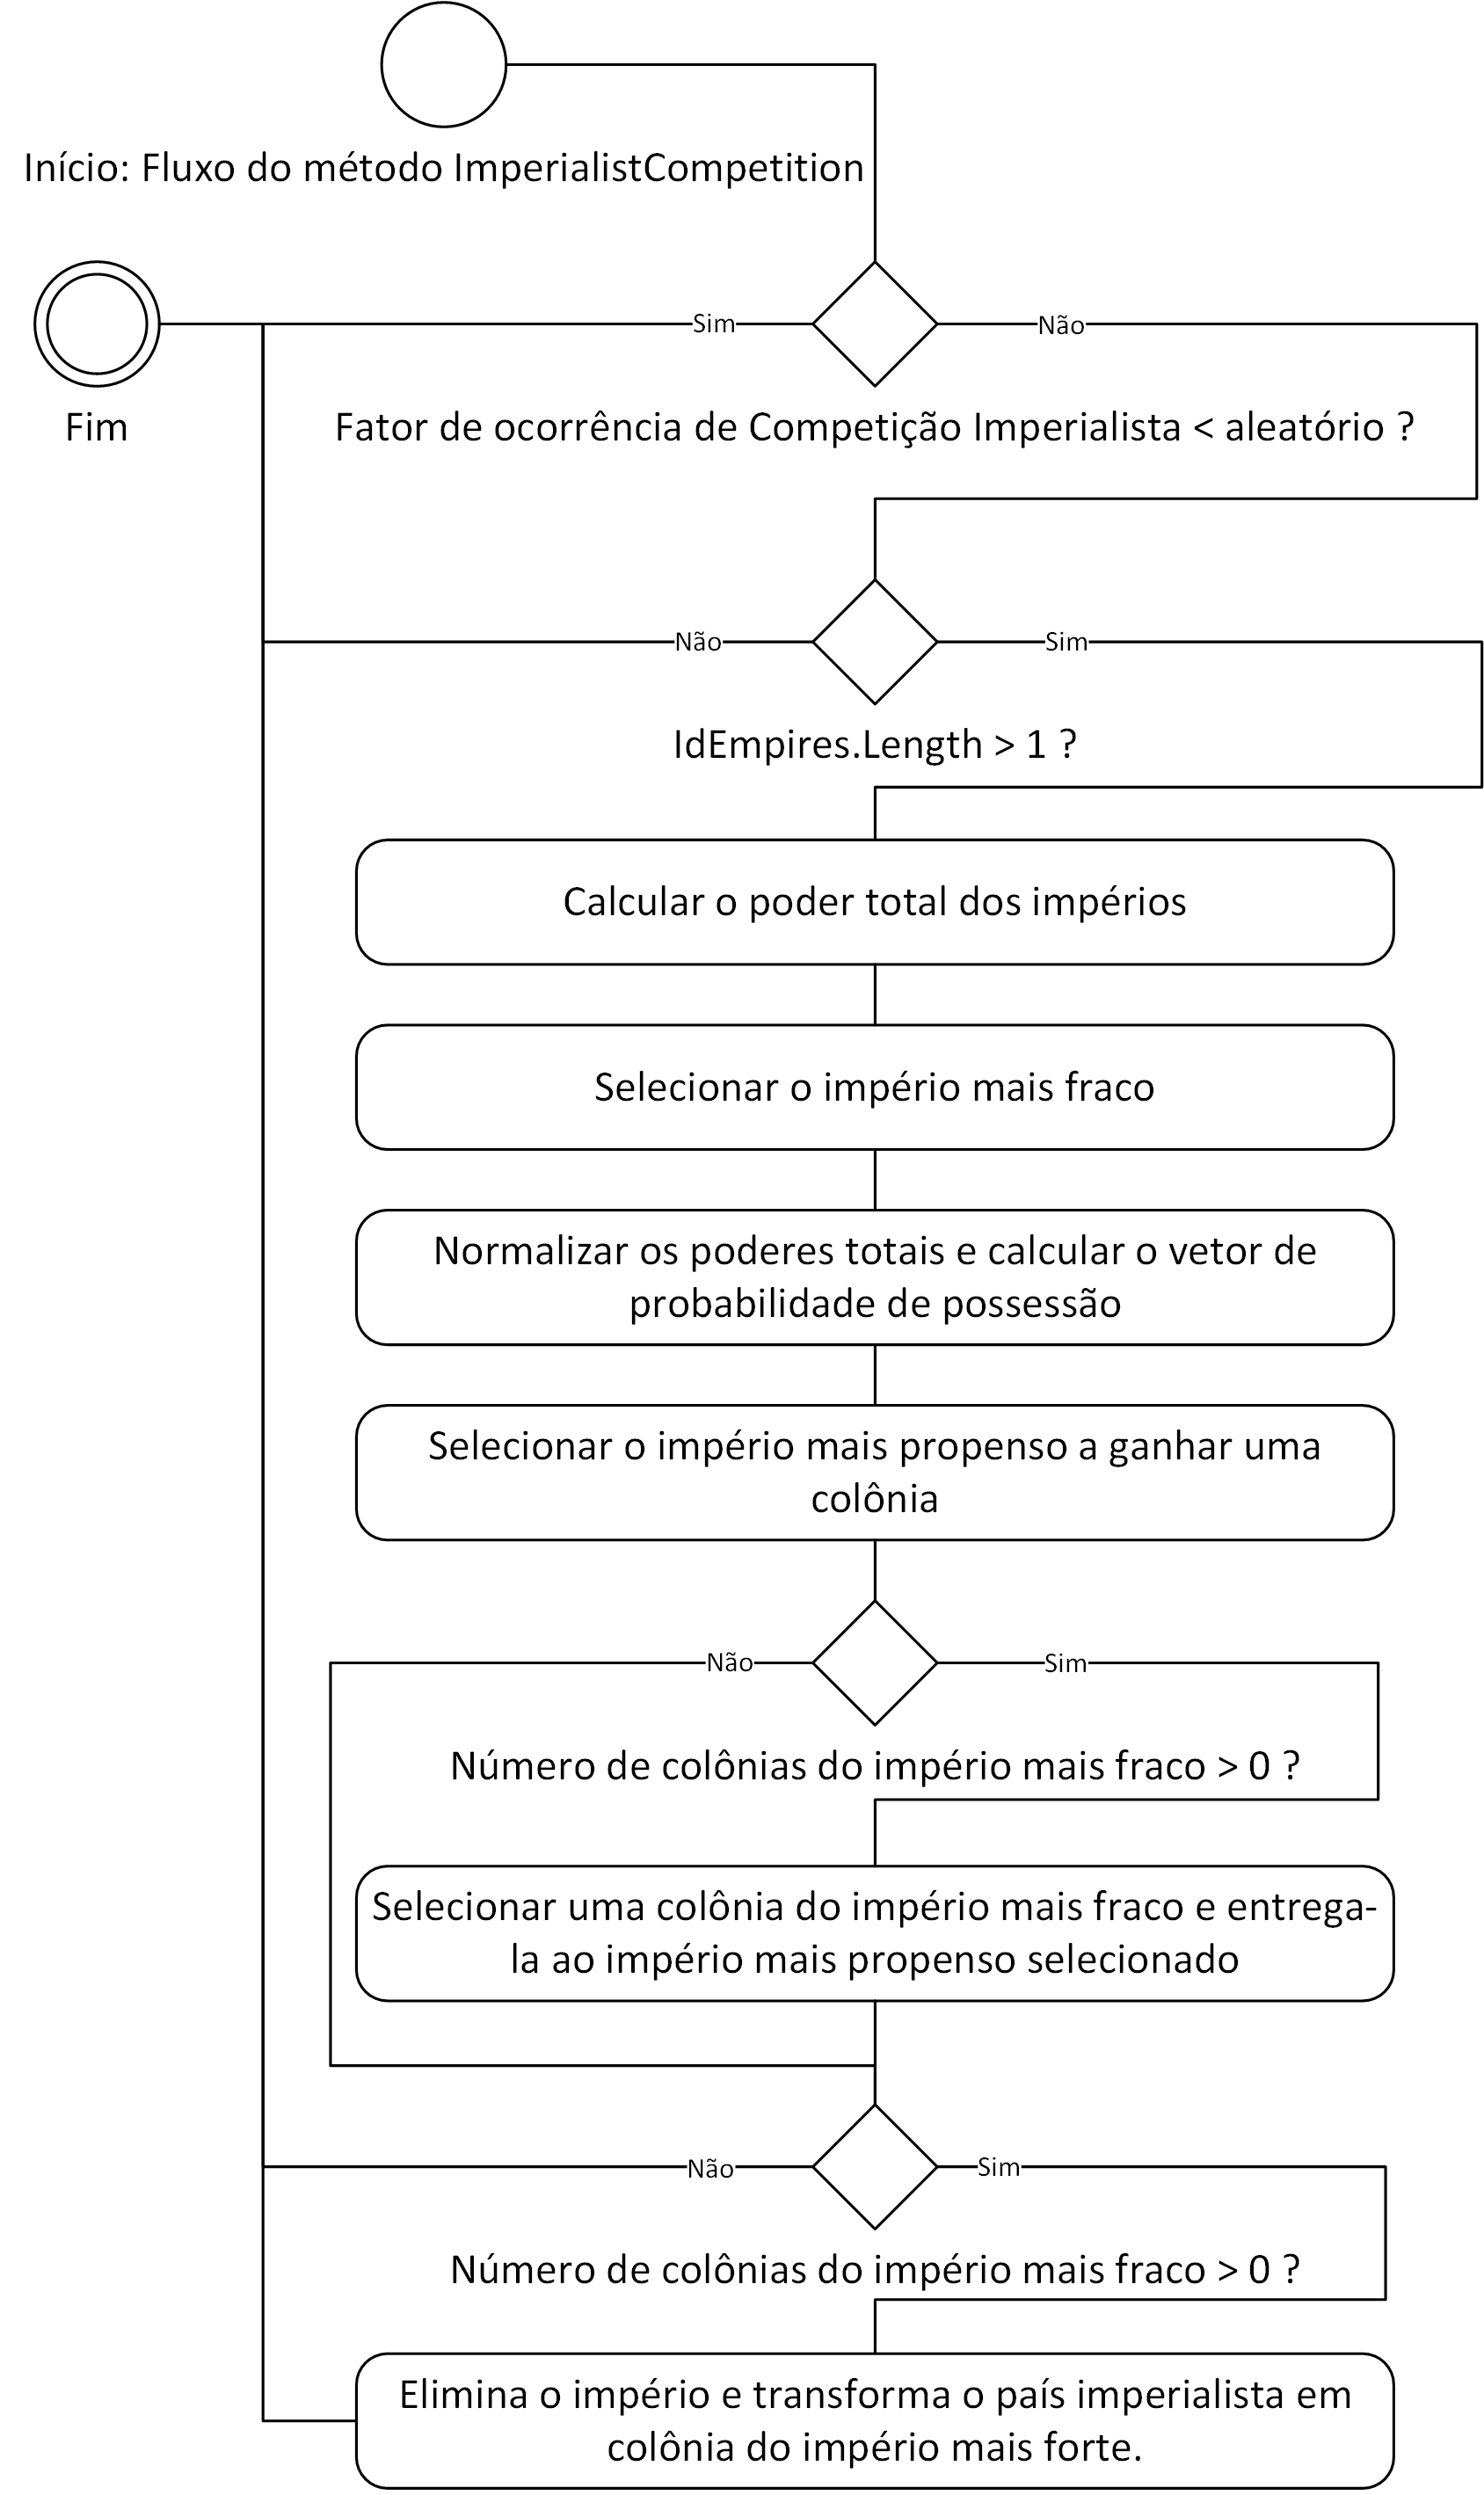
\includegraphics[scale=0.7]{Figuras/Fluxograms-RunMethodImperialistCompetition.png}
	\caption{Fluxograma competição imperialista}
	\label{fig:Fluxograms-RunMethodImperialistCompetition}
	\end{figure}
    
Após terminar a chamada do método \emph{ImperialistCompetition}, conclui-se o \emph{loop} principal incrementando o valor de década. Ao retornar  para o início do \emph{loop}, são verificadas as condições de parada até que alguma delas retorne o valor de parada e o algoritmo finaliza sua execução. Quando o algoritmo termina a execução do método \emph{Run}, a lista de colônias estará posicionada no lugar ótimo para o problema em questão (isto é, seus atributos já estarão otimizados). Os dados podem ser acessados através de suas propriedades públicas pertencentes ao objeto do tipo \emph{ImperialistCompetition} instanciado em memória.

O desenvolvimento do ICA orientado a objetos proporciona principalmente praticidade no que diz respeito a modelagem genérica de problemas, ou seja, qualquer problema que se queira otimizar pode fácil e rapidamente ser implementado para que o ICA consuma os métodos da interface \emph{IFitness} que descreve o problema a ser otimizado. Outra vantagem que a orientação a objetos trouxe foi a organização dos conceitos, de forma que se possa ter um profundo entendimento de como o algoritmo efetua suas operações até que se chegue em soluções ótimas. E por fim, num contexto geral a modelagem do ICA foi pensada para que ele demonstrasse desempenho ótimo, dependendo basicamente do tempo que a função de avaliação leva para executar e nada mais.

Todas estas alterações de otimização do ICA apenas foram possíveis através do desenvolvimento Orientado a Objetos, que permite encapsular as entidades e desenvolver suas lógicas separadas em métodos bem definidos, assim, abstrai-se a solução em objetos capazes de atender e concentrar os aspectos essenciais do contexto (competição imperialista) de uma forma bem definida. Assim, a implementação do ICA permite fácil adaptação a qualquer abordagem ou ambientação de otimização para um dado problema.







\subsection{Exemplos de aplicação do ICA genérico}
\label{Exemplos de aplicação do ICA genérico}

Abaixo apresentam-se dois cenários distintos de implementação do ICA Generalista abordando dois problemas, G1 e G2. O primeiro é uma implementação mais simples, em que a avaliação se dá pela necessidade de minimização da função matemática:

\begin{equation}
\centering
\begin{split}
\text{Problema G1:} \\
& F(x,y) = x \cdot \sin(4 \cdot x)+ 1.1 \cdot y \cdot \sin(2 \cdot y), \\ 
& 0 < x,y < 10, \\ 
& mínimo: f(9.039, 8.6680) = -18.5547.
\end{split}
\end{equation}

A implementação deste problema fica muito simples, pois será um problema de minimização de função matemática dentro de um intervalo fechado, assim, o diagrama de classes simplificado fica como apresentado na Figura \ref{fig:Problems-G1Model}.

\begin{figure}[h]
	\centering
	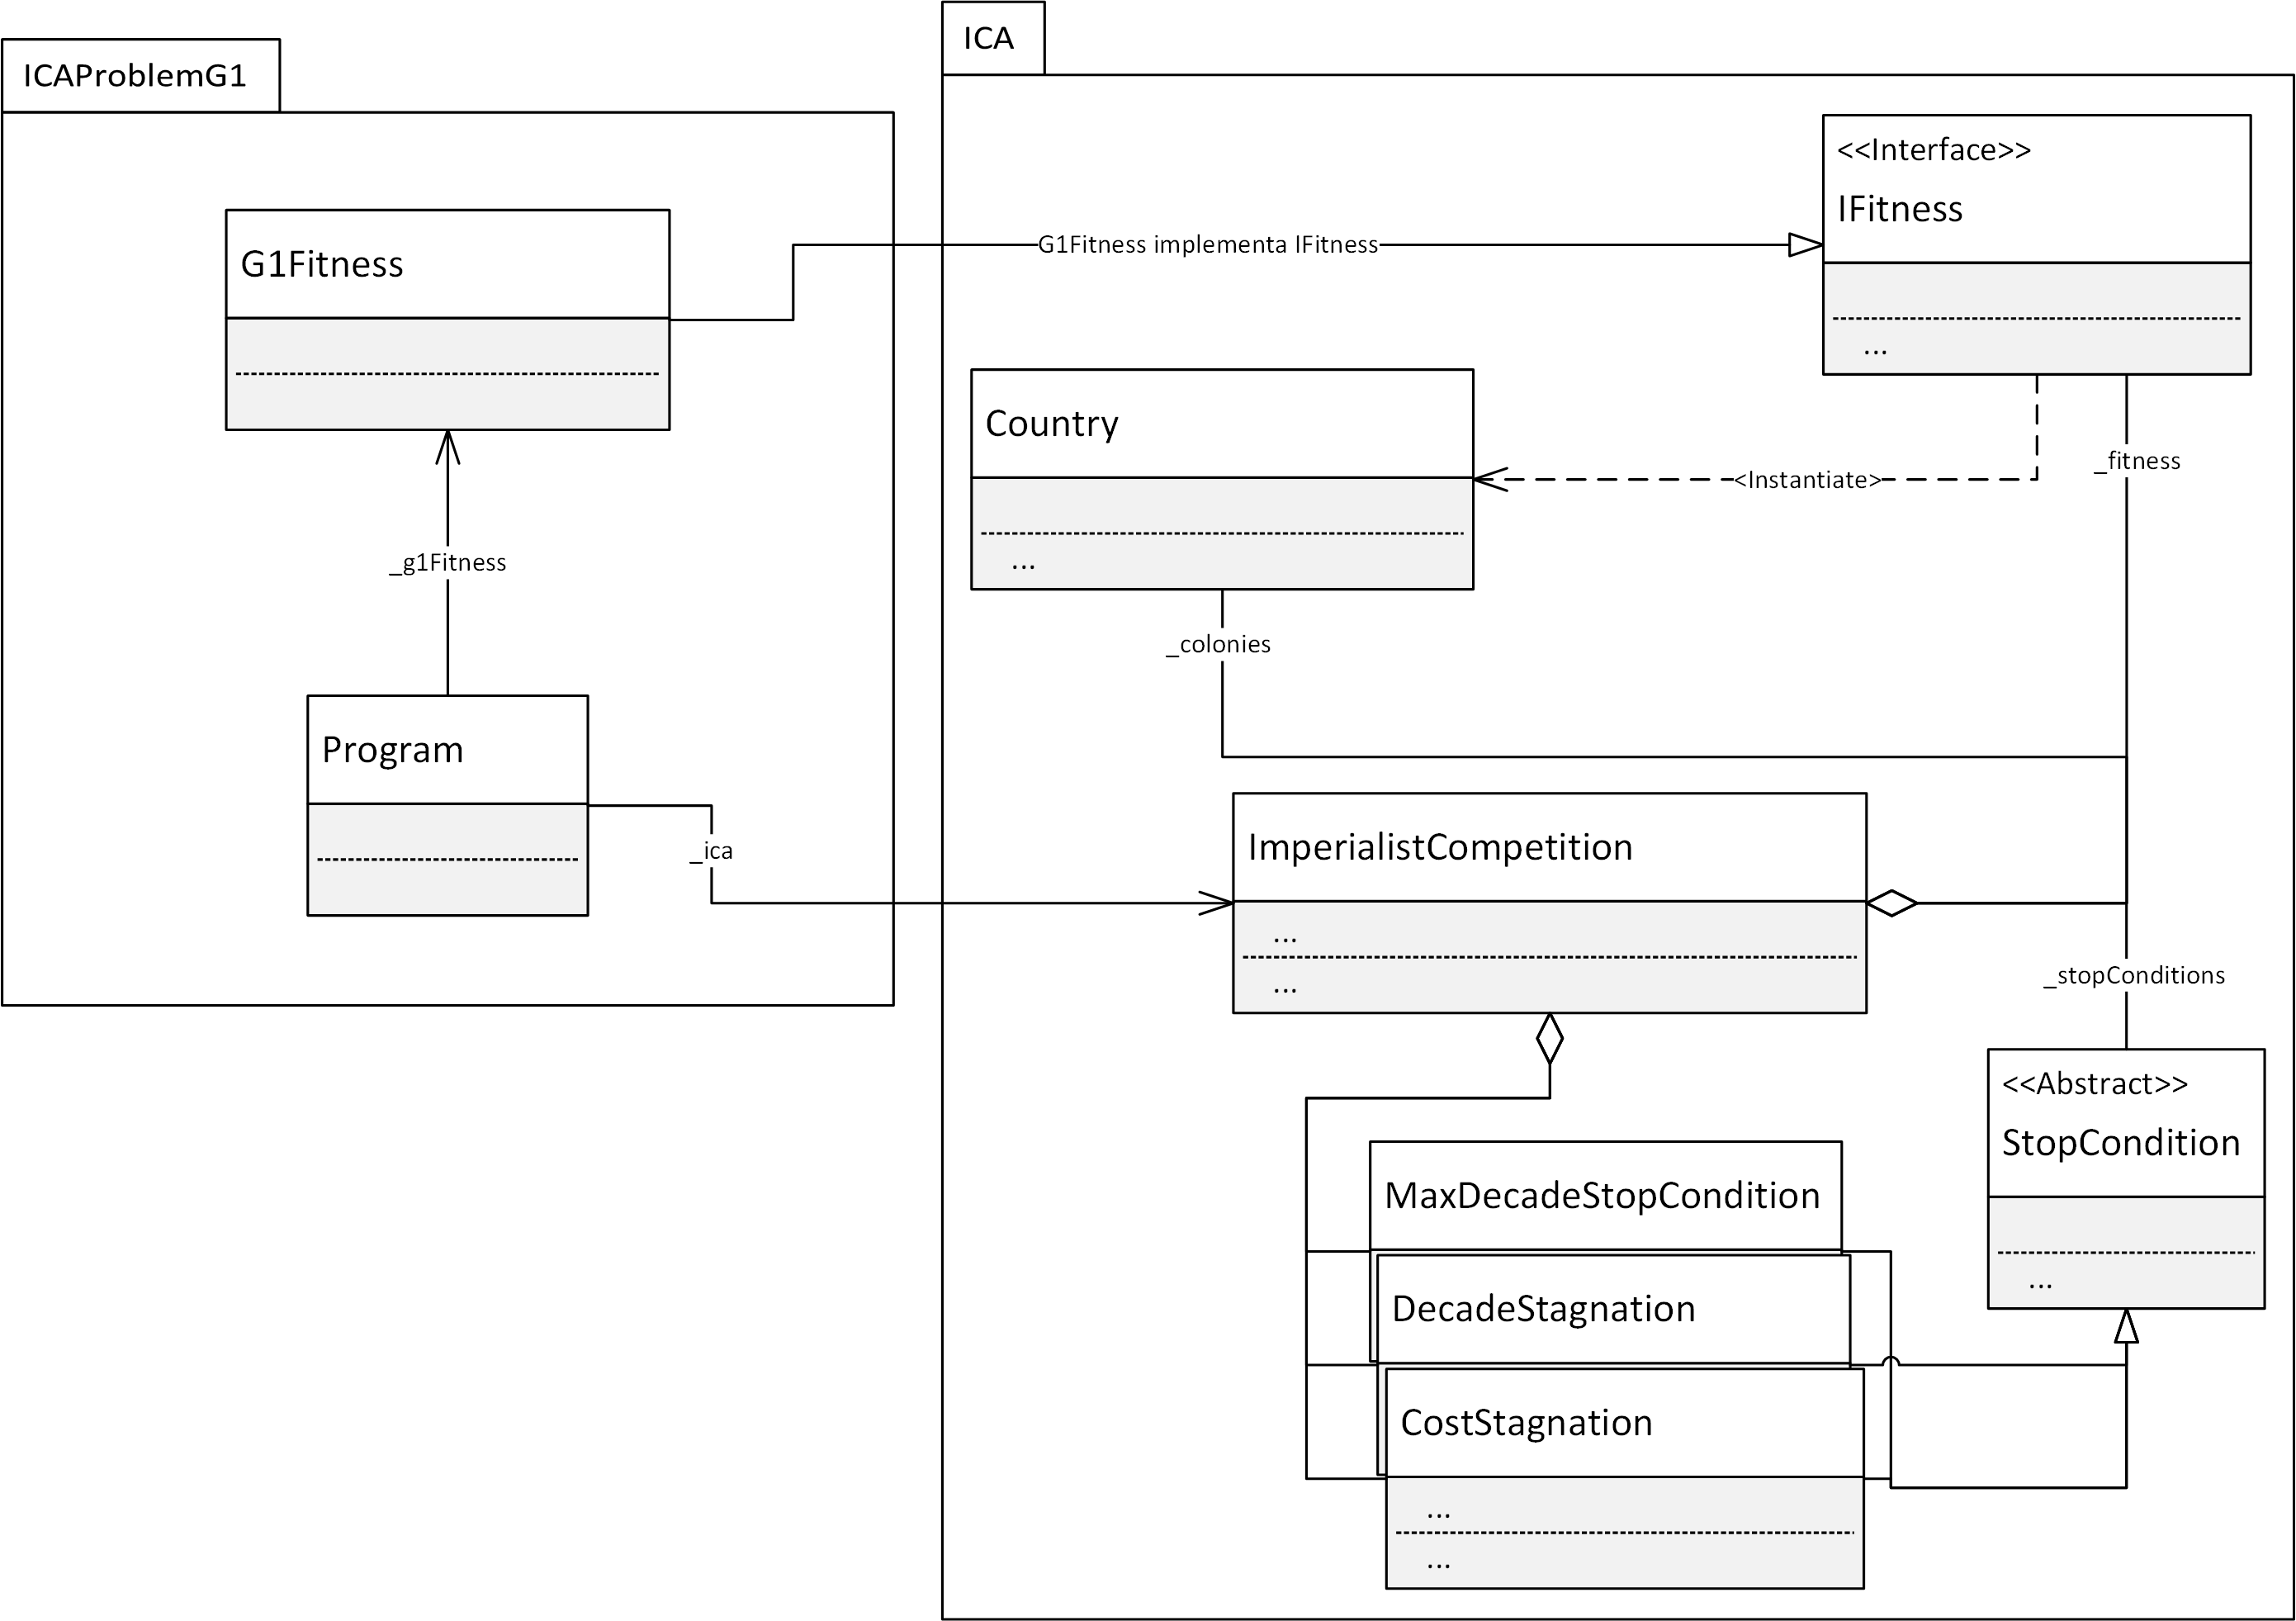
\includegraphics[scale=0.6]{Figuras/Problems-G1Model.png}
	\caption{Diagrama de classes simplificado do problema G1}
	\label{fig:Problems-G1Model}
\end{figure}

No diagrama simplificado é possível observar que a estrutura inicial do ICA não foi alterada. No desenvolvimento da solução foi criada uma classe \emph{G1Fitness} implementando a interface \emph{IFitness}, na qual define o problema implementando os métodos obrigatórios da interface \emph{IFitness}.

A modelagem deste problema para o ICA é simples, pois tem 2 dimensões onde seus limites são fechados entre 0 e 10. Assim, tem-se que o vetor de atributos para cada país será como apresentado na Figura \ref{fig:Problems-G1Vector}.

\begin{figure}[h]
	\centering
	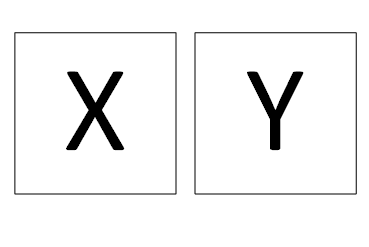
\includegraphics[scale=0.6]{Figuras/Problems-G1Vector.png}
	\caption{Vetor de atributos dos países do problema G1}
	\label{fig:Problems-G1Vector}
\end{figure}

A classe implementada para o problema G1, \emph{G1Fitness}, implementa todos os métodos existentes na interface \emph{IFitness}, sendo assim, a propriedade \emph{Dimensions} apenas retorna o valor 2, pois o problema apresenta duas dimensões(valores de ponto flutuante para \(x\) e para \(y\)). O método \emph{GenerateCountries} não tem nada de especial, apenas cria instâncias simples da classe \emph{Country}, passando os parâmetros necessários no seu construtor padrão, e agrega-as em um vetor para o retorno. E por fim o método \emph{Eval} foi implementado de forma que o custo do país seja o valor da função \(f(x,y)\) tal que \(x = Atributo0\) e \(y = Atributo1\), como descrito no algoritmo \ref{alg:G1Problem}.

\vspace{10px}
\begin{algorithm}[h]
\SetAlgoLined
\KwData{\\ \textbf{ref} element - A referência do país a ser avaliado}
\KwResult{ nenhum valor de retorno, pois altera-se diretamente na referência de element}
x = element.Attributes[0]\;
y = element.Attributes[1]\;
Fxy =\( x \cdot \sin(4.0 \cdot x) + 1.1 \cdot y \cdot \sin(2.0 \cdot y);\)\;
element.Cost = Fxy\;
\caption{ Pseudocódigo método \emph{Eval} do problema G1.}
\label{alg:G1Problem}
\end{algorithm}
\vspace{10px}

Para a apresentação dos resultados foi utilizado o próprio console, e os parâmetros de entrada para o ICA foram: 

Total de países: 128, 

Número de décadas: 512, 

Taxa de revolução: 0.9, 

Taxa de decaimento de revolução: 0.95, 

Coeficiente de assimilação: 0.0001, 

Epsilon: 0.025,

Porcentagem inicial de impérios: 0.15

E no término o melhor indivíduo apresentou os resultados: 

X = 9.0376,

Y = 8.6725,

F(X,Y) = -18.55422.

Este teste apresentou um erro muito menor que 1\%, calculado a seguir: 

\begin{equation}
\begin{split}
e = Abs(Valor Esperado - Valor Obtido ) 
\\= Abs((-18.5547) - (-18.55422)) = 0.00048 \\
e\%= 0.00258695\%
\end{split}
\end{equation}



O problema G2 exige uma função de avaliação mais complexa, e se dá no seguinte cenário: Dadas duas imagens, sendo que a segunda (I') é a imagem resultado da passagem de um filtro de convolução (M) qualquer sobre a primeira imagem(I), o objetivo do ICA é encontrar qual foi o filtro (máscara de convolução) utilizado neste processamento. O nível de complexidade deste problema é altíssimo, por este ser um problema de inversão de uma função que quando aplicada pode ocasionar em perda ou geração de informação ou ruído no seu resultado, tornando impossível a descoberta do filtro de uma forma direta. A princípio, nos exemplos, foram utilizados apenas filtros de ordem 3 e imagens em escala de cinza(I e I'), todos representados por matrizes de valores.

A implementação do problema G2 foi mais complexa, e usa quase todas as novas funcionalidades do ICA descritas neste trabalho. Na Figura \ref{fig:Problems-G2Model} pode-se observar que não só a classe \emph{IFitness} fora estendida, mas também a classe \emph{Country}. O motivo de se estender a classe \emph{Country} foi para demonstrar duas funcionalidades extras, na qual a primeira tem como objetivo armazenar o resultado obtido pela função de avaliação para que se possa fazer uso posterior sem a necessidade de reprocessamento, já a segunda tem como objetivo alterar o funcionamento da função de randomização de todos os atributos do país, que é chamada sempre que se iniciam os países e também quando ocorre a revolução de uma colônia durante a evolução das décadas. 

\begin{figure}[h]
	\centering
	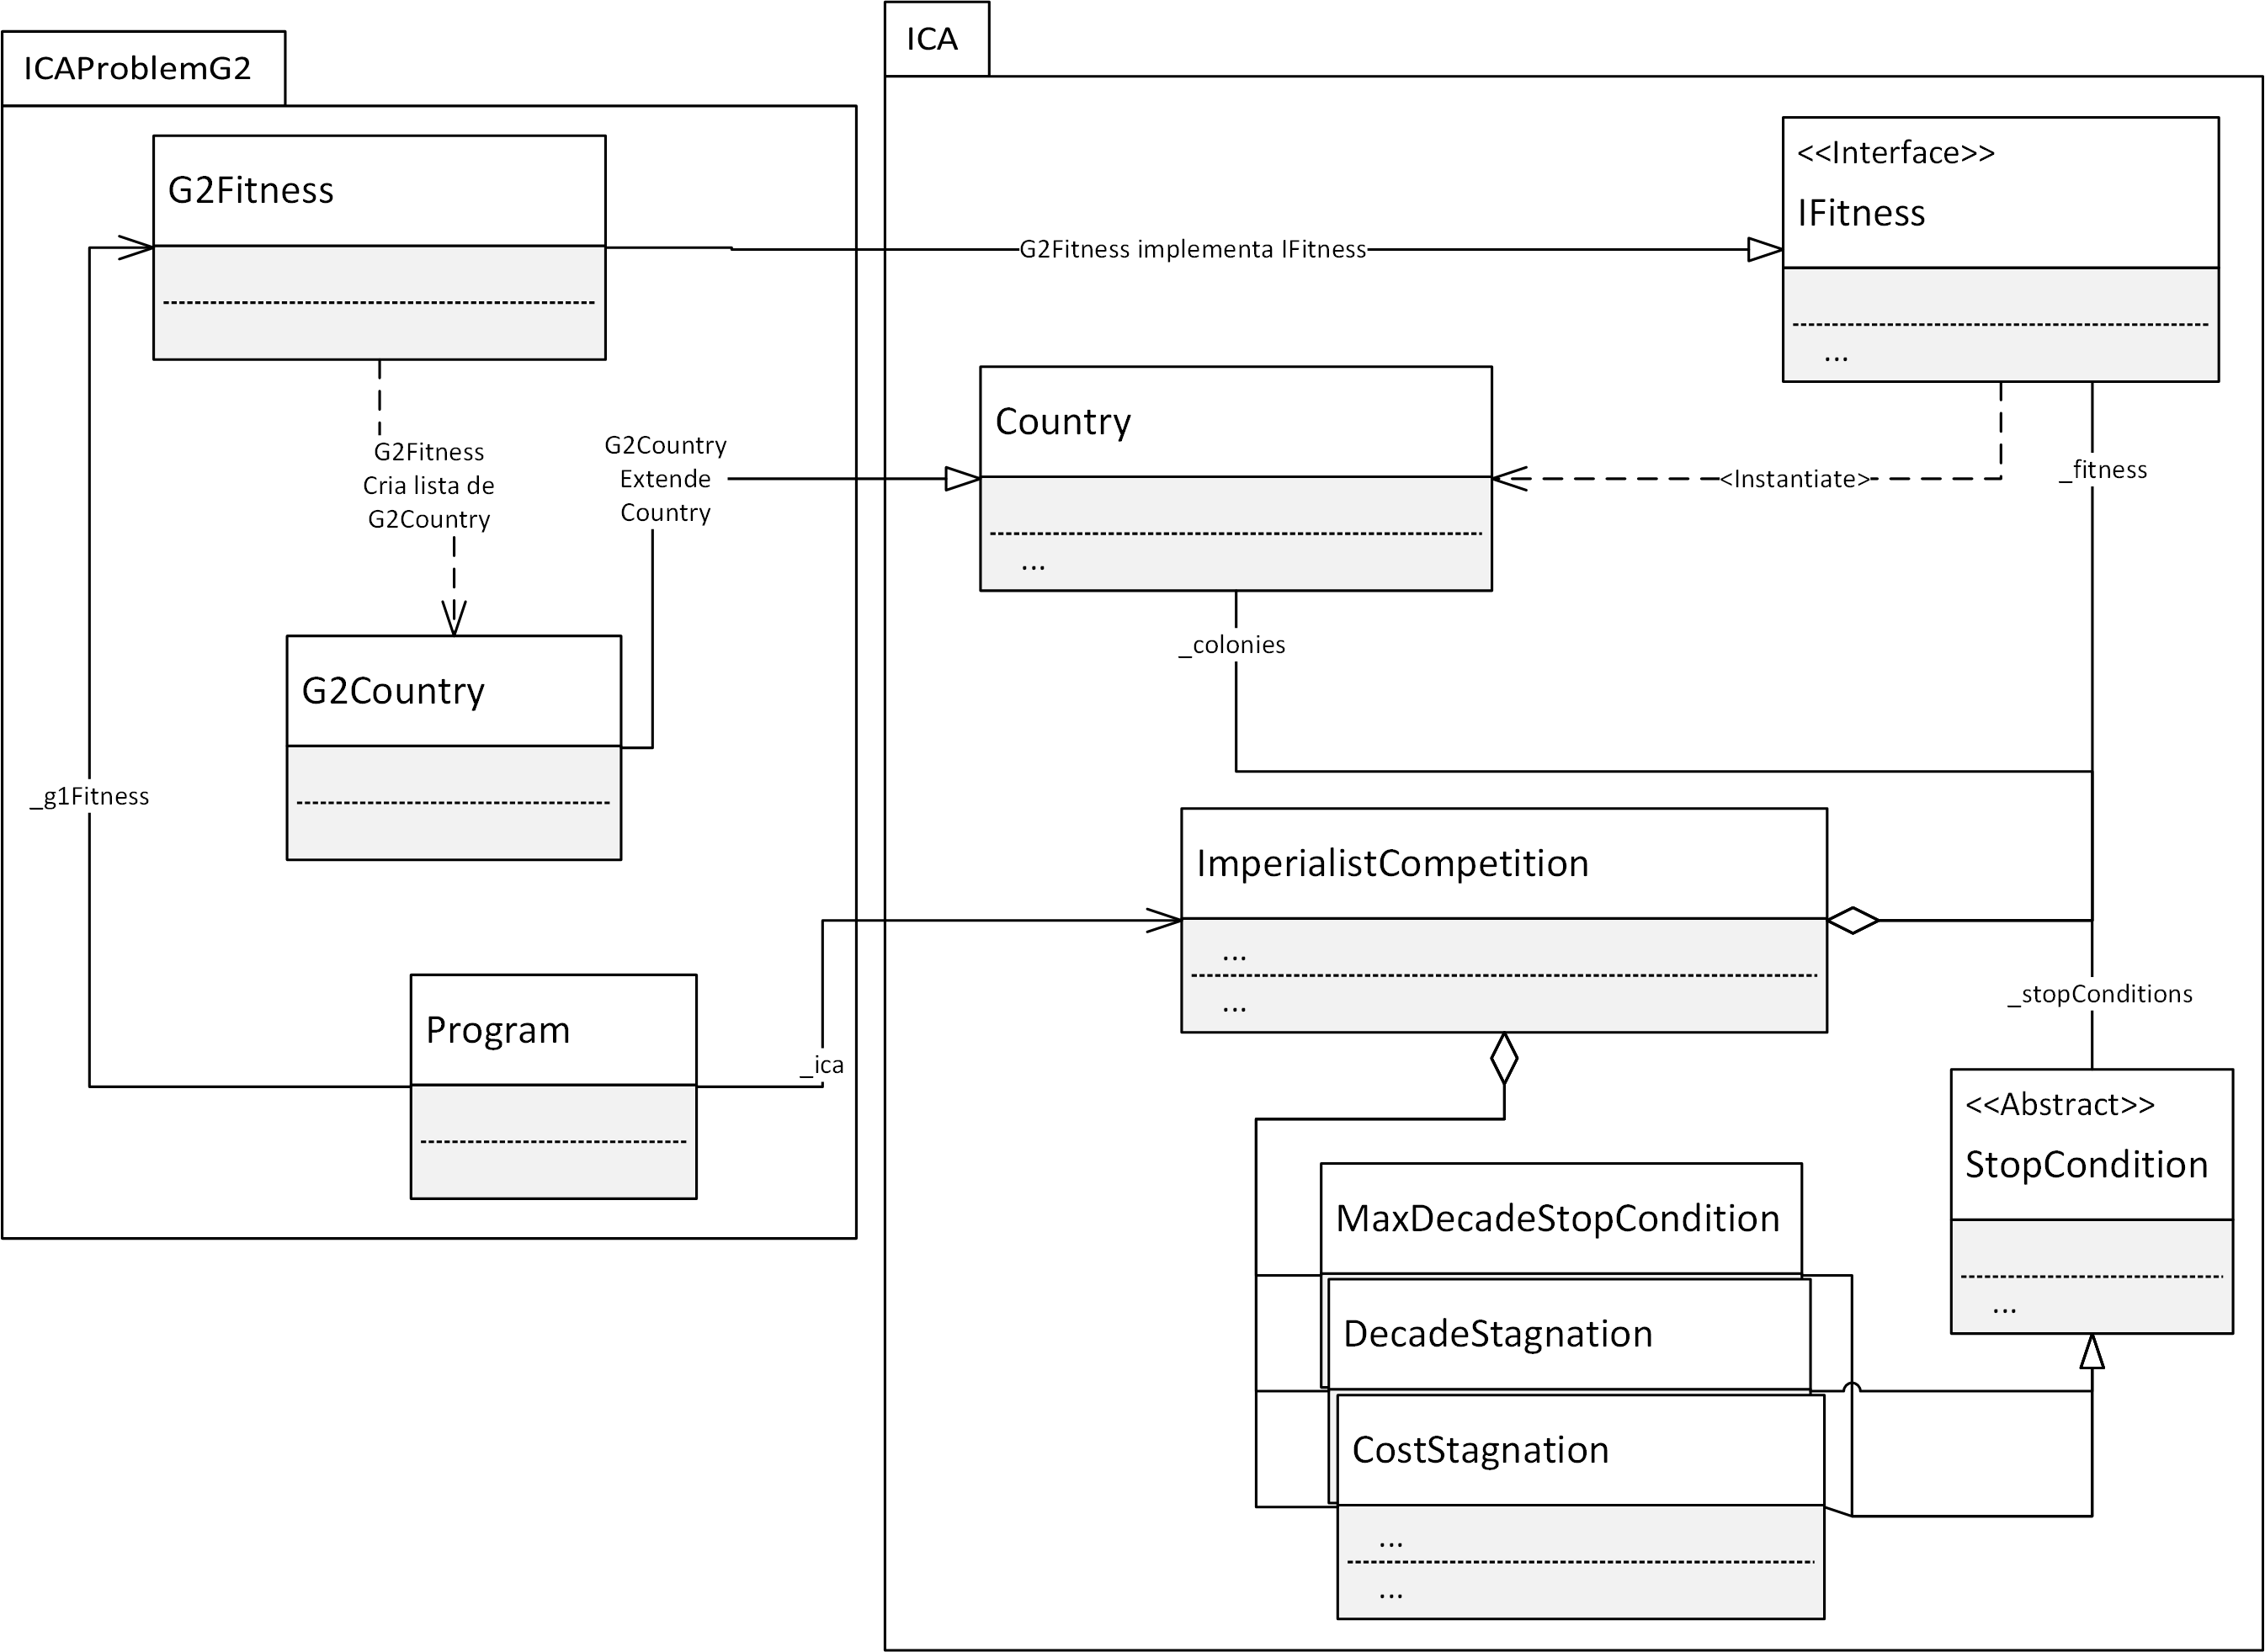
\includegraphics[scale=0.5]{Figuras/Problems-G2Model.png}
	\caption{Diagrama de classes simplificado do problema G2 }
	\label{fig:Problems-G2Model}
\end{figure}

Para que se alcance um resultado satisfatório a modelagem deste problema deve levar em conta, inicialmente, a ordem do filtro e os valores de cada elemento da matriz que representa este filtro. Então, um dos parâmetros definidos na modelagem do problema deve ser a ordem da matriz de convolução, que define quantos atributos os países terão.

Com a ordem estipulada, tem-se que a propriedade \emph{Dimensions} da classe \emph{G2Fitness} retorna a definição do número de dimensões do problema como sendo \(Dimensions = ordem * ordem\). Assim, com o número de dimensões estipulado, para o caso geral de \emph{ordem = n}, o vetor de atributos deve representar todos os elementos da matriz filtro em uma sequência unidimensional representada conforme a Figura \ref{fig:Problems-G2Vector}.

\begin{figure}[h]
	\centering
	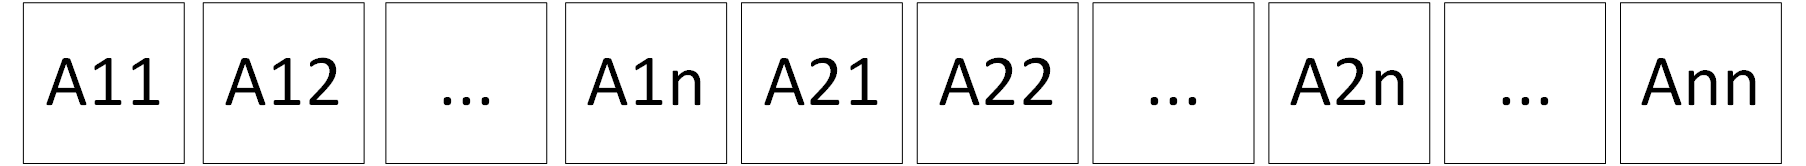
\includegraphics[scale=0.8]{Figuras/Problems-G2Vector.png}
	\caption{Vetor de atributos dos países do problema G2}
	\label{fig:Problems-G2Vector}
\end{figure}

Com o modelo do problema pronto, antes de implementar os métodos da interface \emph{IFitness} na classe \emph{G2Fitness}, estende-se a classe \emph{Country} para a classe \emph{G2Country}, que por sua vez sobrescreve o método \emph{RandomizeAttributes} para utilizar uma função randômica de distribuição normal (substituindo a distribuição anterior, que era uniforme), que por padrão tem \(\mu = 0\) e \(\sigma = 0.269\) (de modo que o valor aleatório retornado varie entre 0 e aproximadamente 1). Outra funcionalidade que a classe \emph{G2Country}  traz é a adição de uma propriedade para se armazenar o resultado que o método \emph{Eval} da classe \emph{G2Fitness} gera, de forma que se possa salvar esta informação durante ou depois do processamento do ICA.

O método \emph{Eval} da classe \emph{G2Fitness} é implementado para avaliar qual matriz de convolução presente em cada país é a que mais se encaixa na utilizada para gerar a imagem resultado (I') a partir da imagem original (I) conforme o Algoritmo \ref{alg:G2Problem}

\begin{algorithm}[h]
\SetAlgoLined
\KwData{
\\ \textbf{ref} element - A referência do país a ser avaliado
\\ \textbf{\emph{static}}  I - Imagem original
\\ \textbf{\emph{static}}  I' - Imagem resultado
}
\KwResult{ nenhum valor de retorno, pois altera-se diretamente na referência de element}
Transformar os atributos do país em uma matriz de convolução (M)\;
Efetuar a operação de convolução entre a imagem original (I) e a matriz de convolução (M), obtendo a imagem resultante (R) \;
Calcular a diferença absoluta entre todos os pontos da imagem resultante (R) e a imagem resultado (I'), e armazenar a soma em (d)\;
element.Cost = d\;
element.resultado = R\;
\caption{ Pseudocódigo método \emph{Eval} do problema G1.}
\label{alg:G2Problem}
\end{algorithm}

Durante os testes foi utilizada uma mesma imagem para dois filtros diferentes. Os dois filtros utilizados são o desfoque gaussiano e detecção de borda, apresentados respectivamente com sua aplicação na Figura \ref{fig:Problems-G2Convolution}.

\begin{figure}[h]
	\centering
	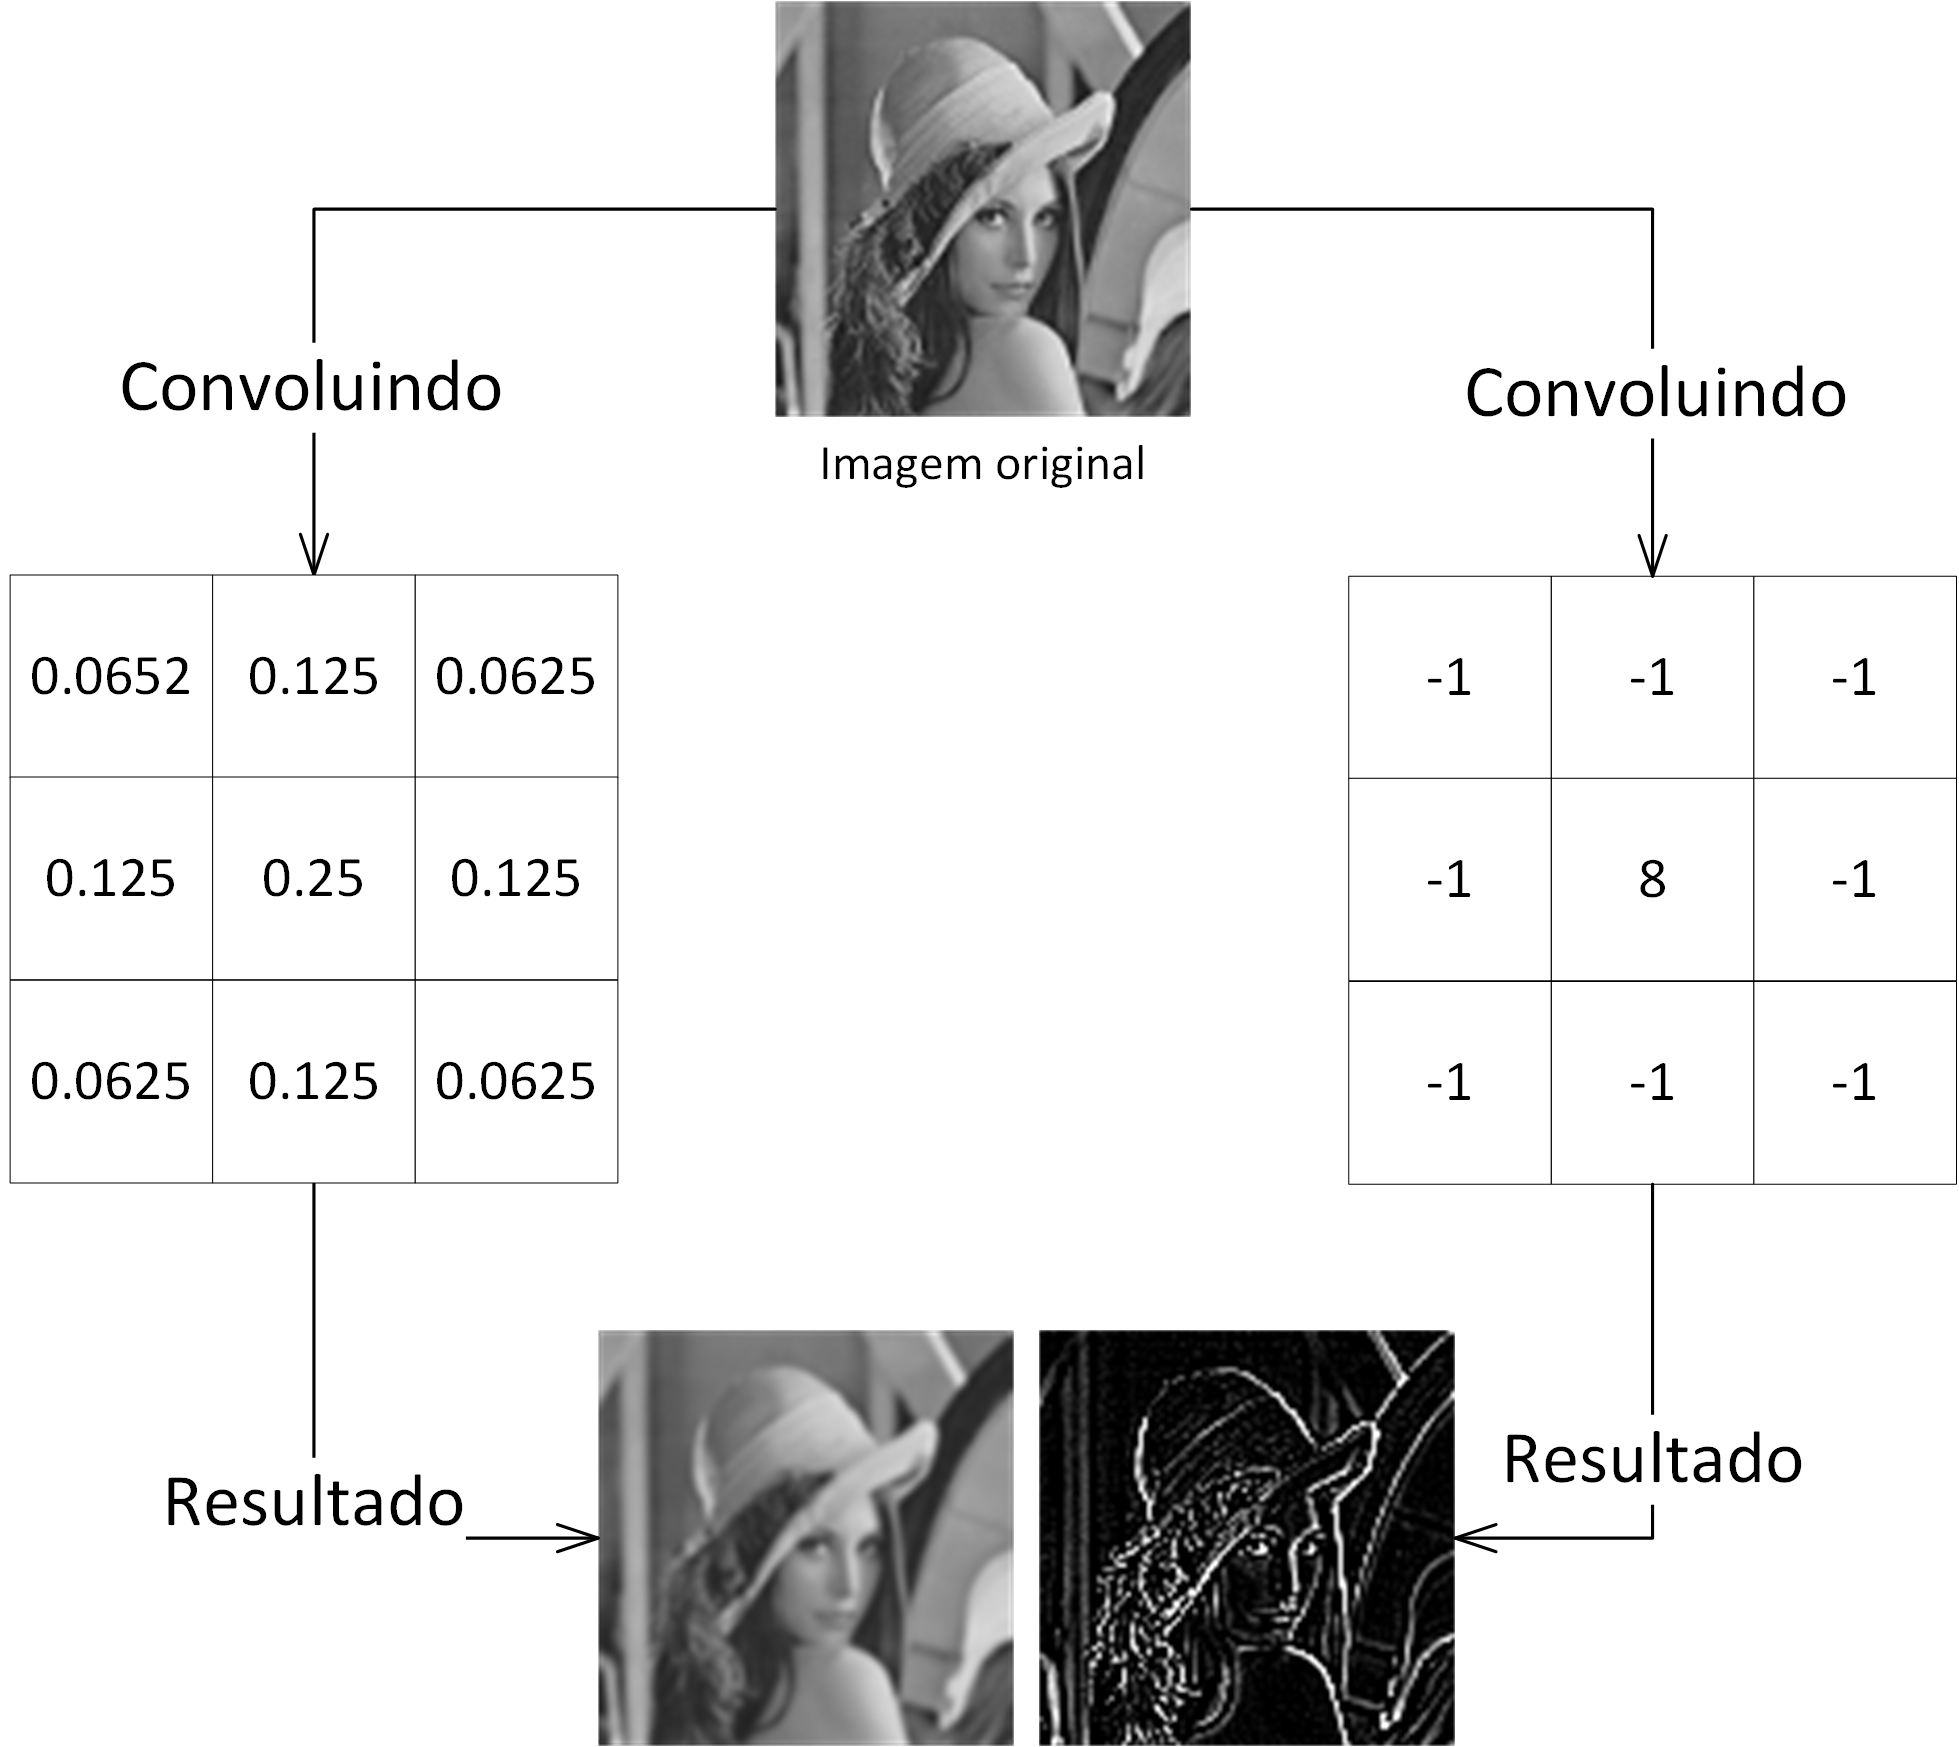
\includegraphics[scale=0.6]{Figuras/Problems-G2Convolution.png}
	\caption{Exemplo Problema G2}
	\label{fig:Problems-G2Convolution}
\end{figure}

Para que o ICA possa encontrar estes dois filtros, ambos tiveram como entrada inicial os mesmos parâmetros, diferenciando-se apenas na imagem resultado e nos limites dos atributos. Os parâmetros de entrada que que foram configurados na inicialização do ICA foram:

Total de países: 64, 

Número máximo de décadas: 2048, 

Taxa de revolução: 0.99, 

Taxa de decaimento de revolução: 0.9999, 

Coeficiente de assimilação: 2, 

Epsilon: 0.025, 

Porcentagem inicial de impérios: 0.15. 

Já os limites, para o filtro de desfoque gaussiano foi escolhido um intervalo entre 0 e 1 para todos os atributos, e para o filtro de detecção de bordas foi escolhido o limite entre -2 e 10 para todos os atributos.

Os demais valores foram mantidos como padrão e podem ser consultados no Anexo1

Os resultados apresentados pela busca de ambos os filtros foram muito bons, e se aproximaram muito do original, como mostrado a seguir na Figura \ref{fig:Problems-G2Results}.

\begin{figure}[h]
	\centering
	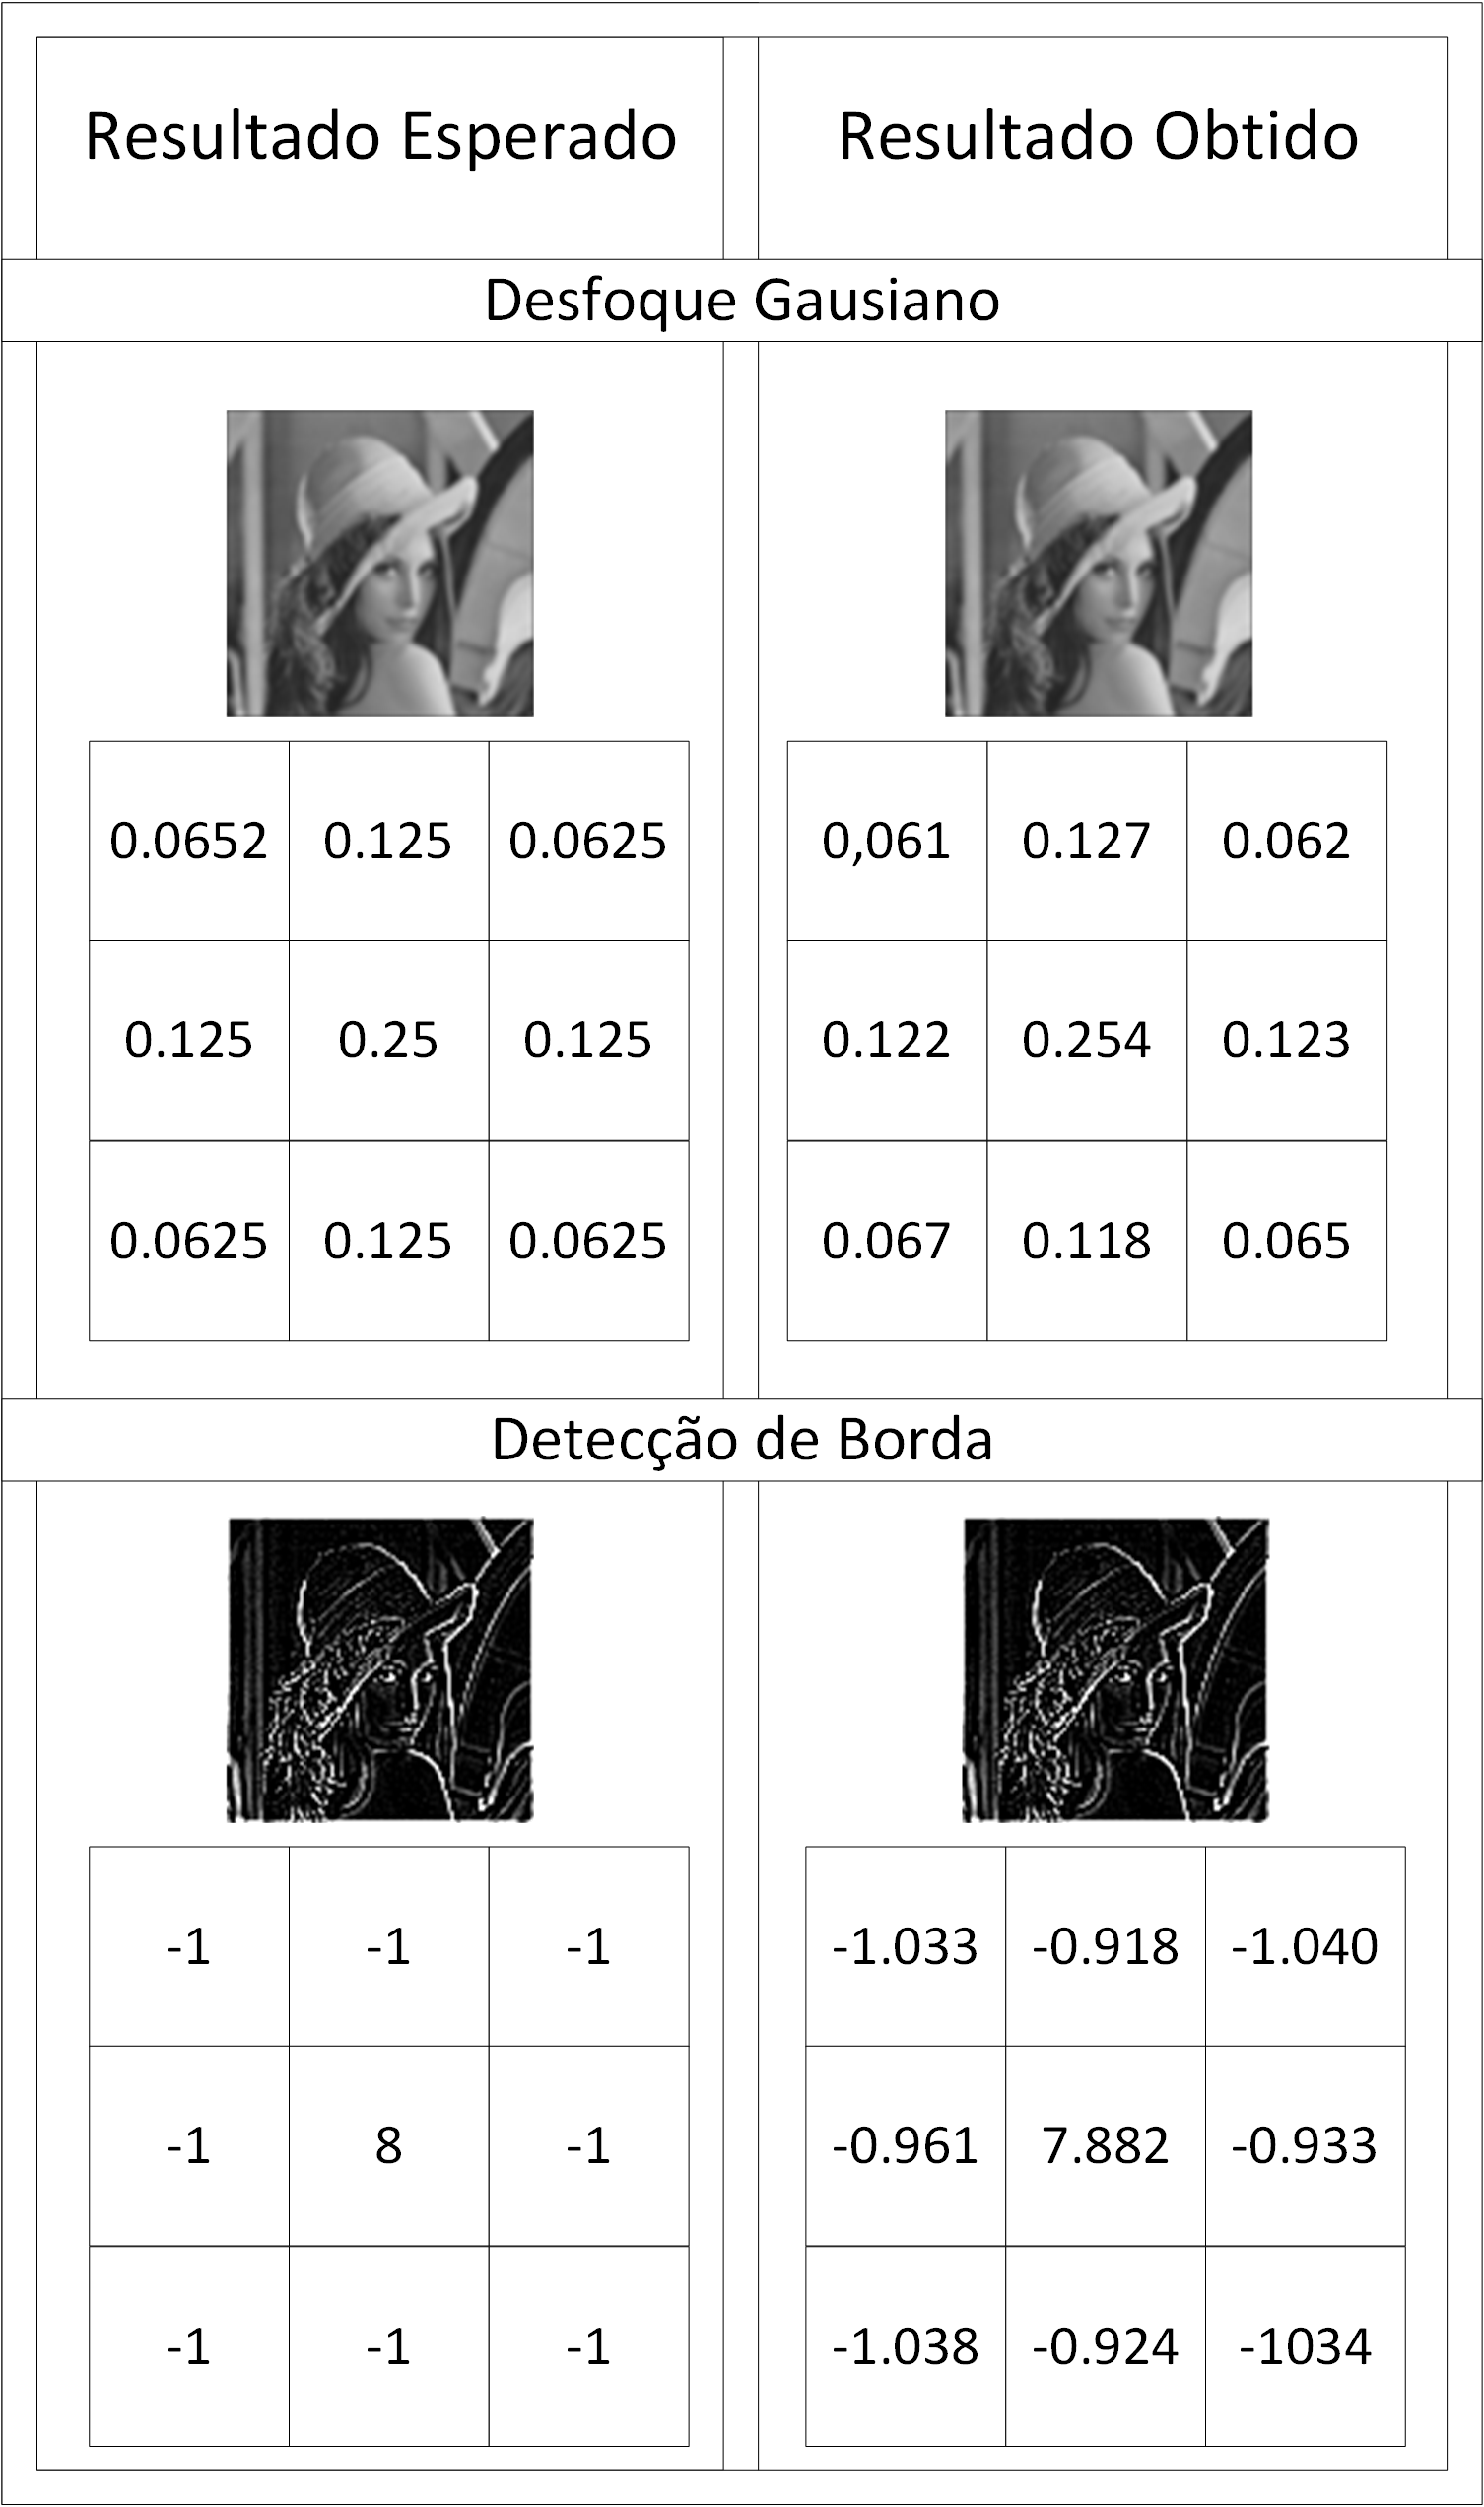
\includegraphics[scale=0.9]{Figuras/Problems-G2Results.png}
	\caption{Resultados do problema G2}
	\label{fig:Problems-G2Results}
\end{figure}

Observa-se que apesar dos resultados dos filtros não atingirem a exatidão, estes chegam muito próximo do resultado esperado e geram imagens indistinguíveis a olho nu. As imagens resultado possuem um erro percentual médio de 0.0471\% e 0.3342\% para as imagens originais geradas a partir do filtro de desfoque gaussiano e de detecção de bordas respectivamente.  

Assim concluímos os exemplos demonstrando a praticidade com que a generalização traz para a modelagem de problemas completamente diferentes, mantendo a estrutura principal do algoritmo inalterada, de modo a adicionar tais problemas como se fossem módulos encapsulados os quais são consumidos e processados pelo ICA.









\section{Análise da operação de movimento do ICA}
\label{Análise da operação de movimento do ICA}


Antes de apresentar cada alteração na operação de movimentação, foi definido um problema que será usado como referência para ambientalizar e ilustrar o entendimento, tanto da operação de movimento citada originalmente, quanto das operações de movimento alteradas apresentadas neste trabalho. O problema P1 em questão refere-se a minimização da função esfera dentro de um intervalo fechado e bidimensional, como mostra a equação \ref{eq:ProblemP1-SphereFunction}.  

Serão apresentadas várias figuras contendo diversos elementos relacionados ao problema, de modo que a estrela vermelha representa a posição em que o país imperialista se encontra, os pontos azuis ligados por linhas representam uma colônia se movendo em direção ao seu país imperialista durante as décadas e a coloração do fundo da imagem, em escalas de cinza, é uma plotagem da função em questão, neste caso da função esfera, que encontra-se no espaço bidimensional dentro do intervalo \(\left[-10, 10\right]\) tanto para \(x\) quanto para \(y\). Esta função foi escolhida, além de ser bem comum, por ter seu mínimo global bem definido e único para este intervalo.

\begin{equation}
f(x,y) = x \cdot x + y \cdot y, \\ x:[-10,10], \\y:[-10,10]
\label{eq:ProblemP1-SphereFunction}
\end{equation}

Inicialmente é preciso entender o que ocorre durante o processo evolutivo do ICA, então, para estes exemplos a funcionalidade de possessão imperial, a qual ocorre quando uma colônia mais forte que seu país imperialista toma o poder para si, foi desabilitada (exceto alguns casos, detalhados mais adiante), de modo que quando uma colônia passar por uma posição de custo menor ela não tome o império para si, além disso, o valor de \(\beta\) utilizado é menor que 1, a taxa de revolução colonial fora configurada como 0, evitando que países tenham seus atributos sorteados novamente, e, por fim, o espaço de busca será explorado por apenas uma colônia junto de um país imperialista, que irão formar um império contendo apenas dois países. A posição inicial da colônia é definida como \((-8,-5)\) e a posição inicial do país imperialista é definida como \((-2,-2)\), mesmo sabendo que o ponto ótimo será o ponto \((0,0)\) e o número máximo de décadas é 40.

A forma como as colônias se movem em direção ao seu imperialista é definida pelo resultado de um valor aleatório proporcional a distância entre cada atributo da colônia em relação aos atributos do país imperialista, e de forma independente dos limites de cada dimensão, tal que, este valor aleatório altera cada atributo na mesma proporção. Assim, pode-se dizer que este valor aleatório representa o tamanho do ‘passo’ que uma colônia dará em direção ao seu país imperialista (lembrando que este valor aleatório é gerado uniformemente no intervalo \(\left[0,\beta\right]\) como mostra a equação \ref{eq:ica7}.


A Figura \ref{fig:Movimento_Linear} ilustra o movimento linear de uma colônia em direção ao seu país imperialista sem a adição de ruído no movimento. Este ruído no movimento se dá pela alteração de cada atributo da colônia somando um valor aleatório, gerado de forma uniforme, e chamado \(\theta\) como mostrado na equação \ref{eq:ica9}. Observe que não foi encontrado o melhor resultado, o qual estaria na posição \((0,0)\) para a solução do problema, apenas houve uma convergência para a mesma posição do império, pois o ruído fora desabilitado para esta demonstração.

\begin{figure}[h]
	\centering
	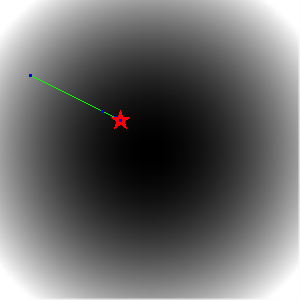
\includegraphics[scale=1]{Figuras/Movimento_Linear.png}
	\caption{Movimento Linear }
	\label{fig:Movimento_Linear}
\end{figure}

Como dito anteriormente, o movimento de uma colônia em direção ao seu país imperialista tem como objetivo principal explorar o espaço de busca para encontrar soluções melhores. O problema de se mover linearmente uma colônia em direção ao seu país imperialista, sem a adição de um ruído, é o mesmo que limitar a busca por soluções melhores dentro de problemas mais complexos, podendo, ao fim das décadas, não chegar ao mínimo global (solução ótima), como pode ser visto na Figura \ref{fig:Movimento_Linear}. Porém o fato da solução não convergir para o mínimo global não significa, neste caso, que a solução estagnou-se em um mínimo local, mas sim que o algoritmo é incapaz de evoluir para a melhor solução por não possuir recursos (adição de ruído durante o movimento) para isto. Então é interessante a adição de um ruído neste movimento, de forma que o espaço de busca seja melhor explorado pela colônia enquanto ela se movimenta em direção ao seu império, como mostra o item \(a\) da Figura \ref{fig:Movimento_Original}. No capítulo \ref{Metodologia} este ruído é definido por \(\theta\), que define um intervalo para a geração de um número aleatório dentro do intervalo \( \left[ -\gamma,\gamma \right]\) que é adicionado a cada atributo. 

O grande problema neste método de inserção de ruídos da forma como é apresentado é a não garantia de proporcionalidade em relação ao espaço de busca de cada atributo, podendo, em um problema mais complexo e com limites diferentes para cada atributo, ter o ruído variando demais em uma dimensão com limites mais apertados, mas ser insignificante em limites de intervalo muito amplo. Além de que com a adição de ruído desta maneira não é possível que a convergência para o cenário ideal (todas as colônias na mesma posição que seu país imperialista ) ocorra.  Os três primeiros itens da Figura \ref{fig:Movimento_Original} \((a, b, c)\), representam o movimento colonial tendo os ruídos definidos com \(\gamma\) valendo respectivamente \(\left(\frac{\pi}{4}\right)\), como descrito por \citeauthor{atashpaz2007imperialist} em \cite{atashpaz2007imperialist}, \(\left(\pi\right)\) e \(\left(4\cdot \pi\right)\). Observa-se que para o item \(a\), existe uma quantidade de ruído pequena, que é aceitável, e que poderia estar levando o império em direção ao mínimo global caso o mecanismo de tomada de poder estivesse habilitado. Já os itens \(b\) e \(c\) apresentam um significativo aumento no ruído, podendo, também, levar à melhor solução, porém esta variação é muito grande e, consequentemente, faz com que a busca pela solução ótima tenda a ser mais aleatória do que direcionada, podendo fazer com que a solução ótima nunca seja atingida.  

\begin{figure}[h]
	\centering
	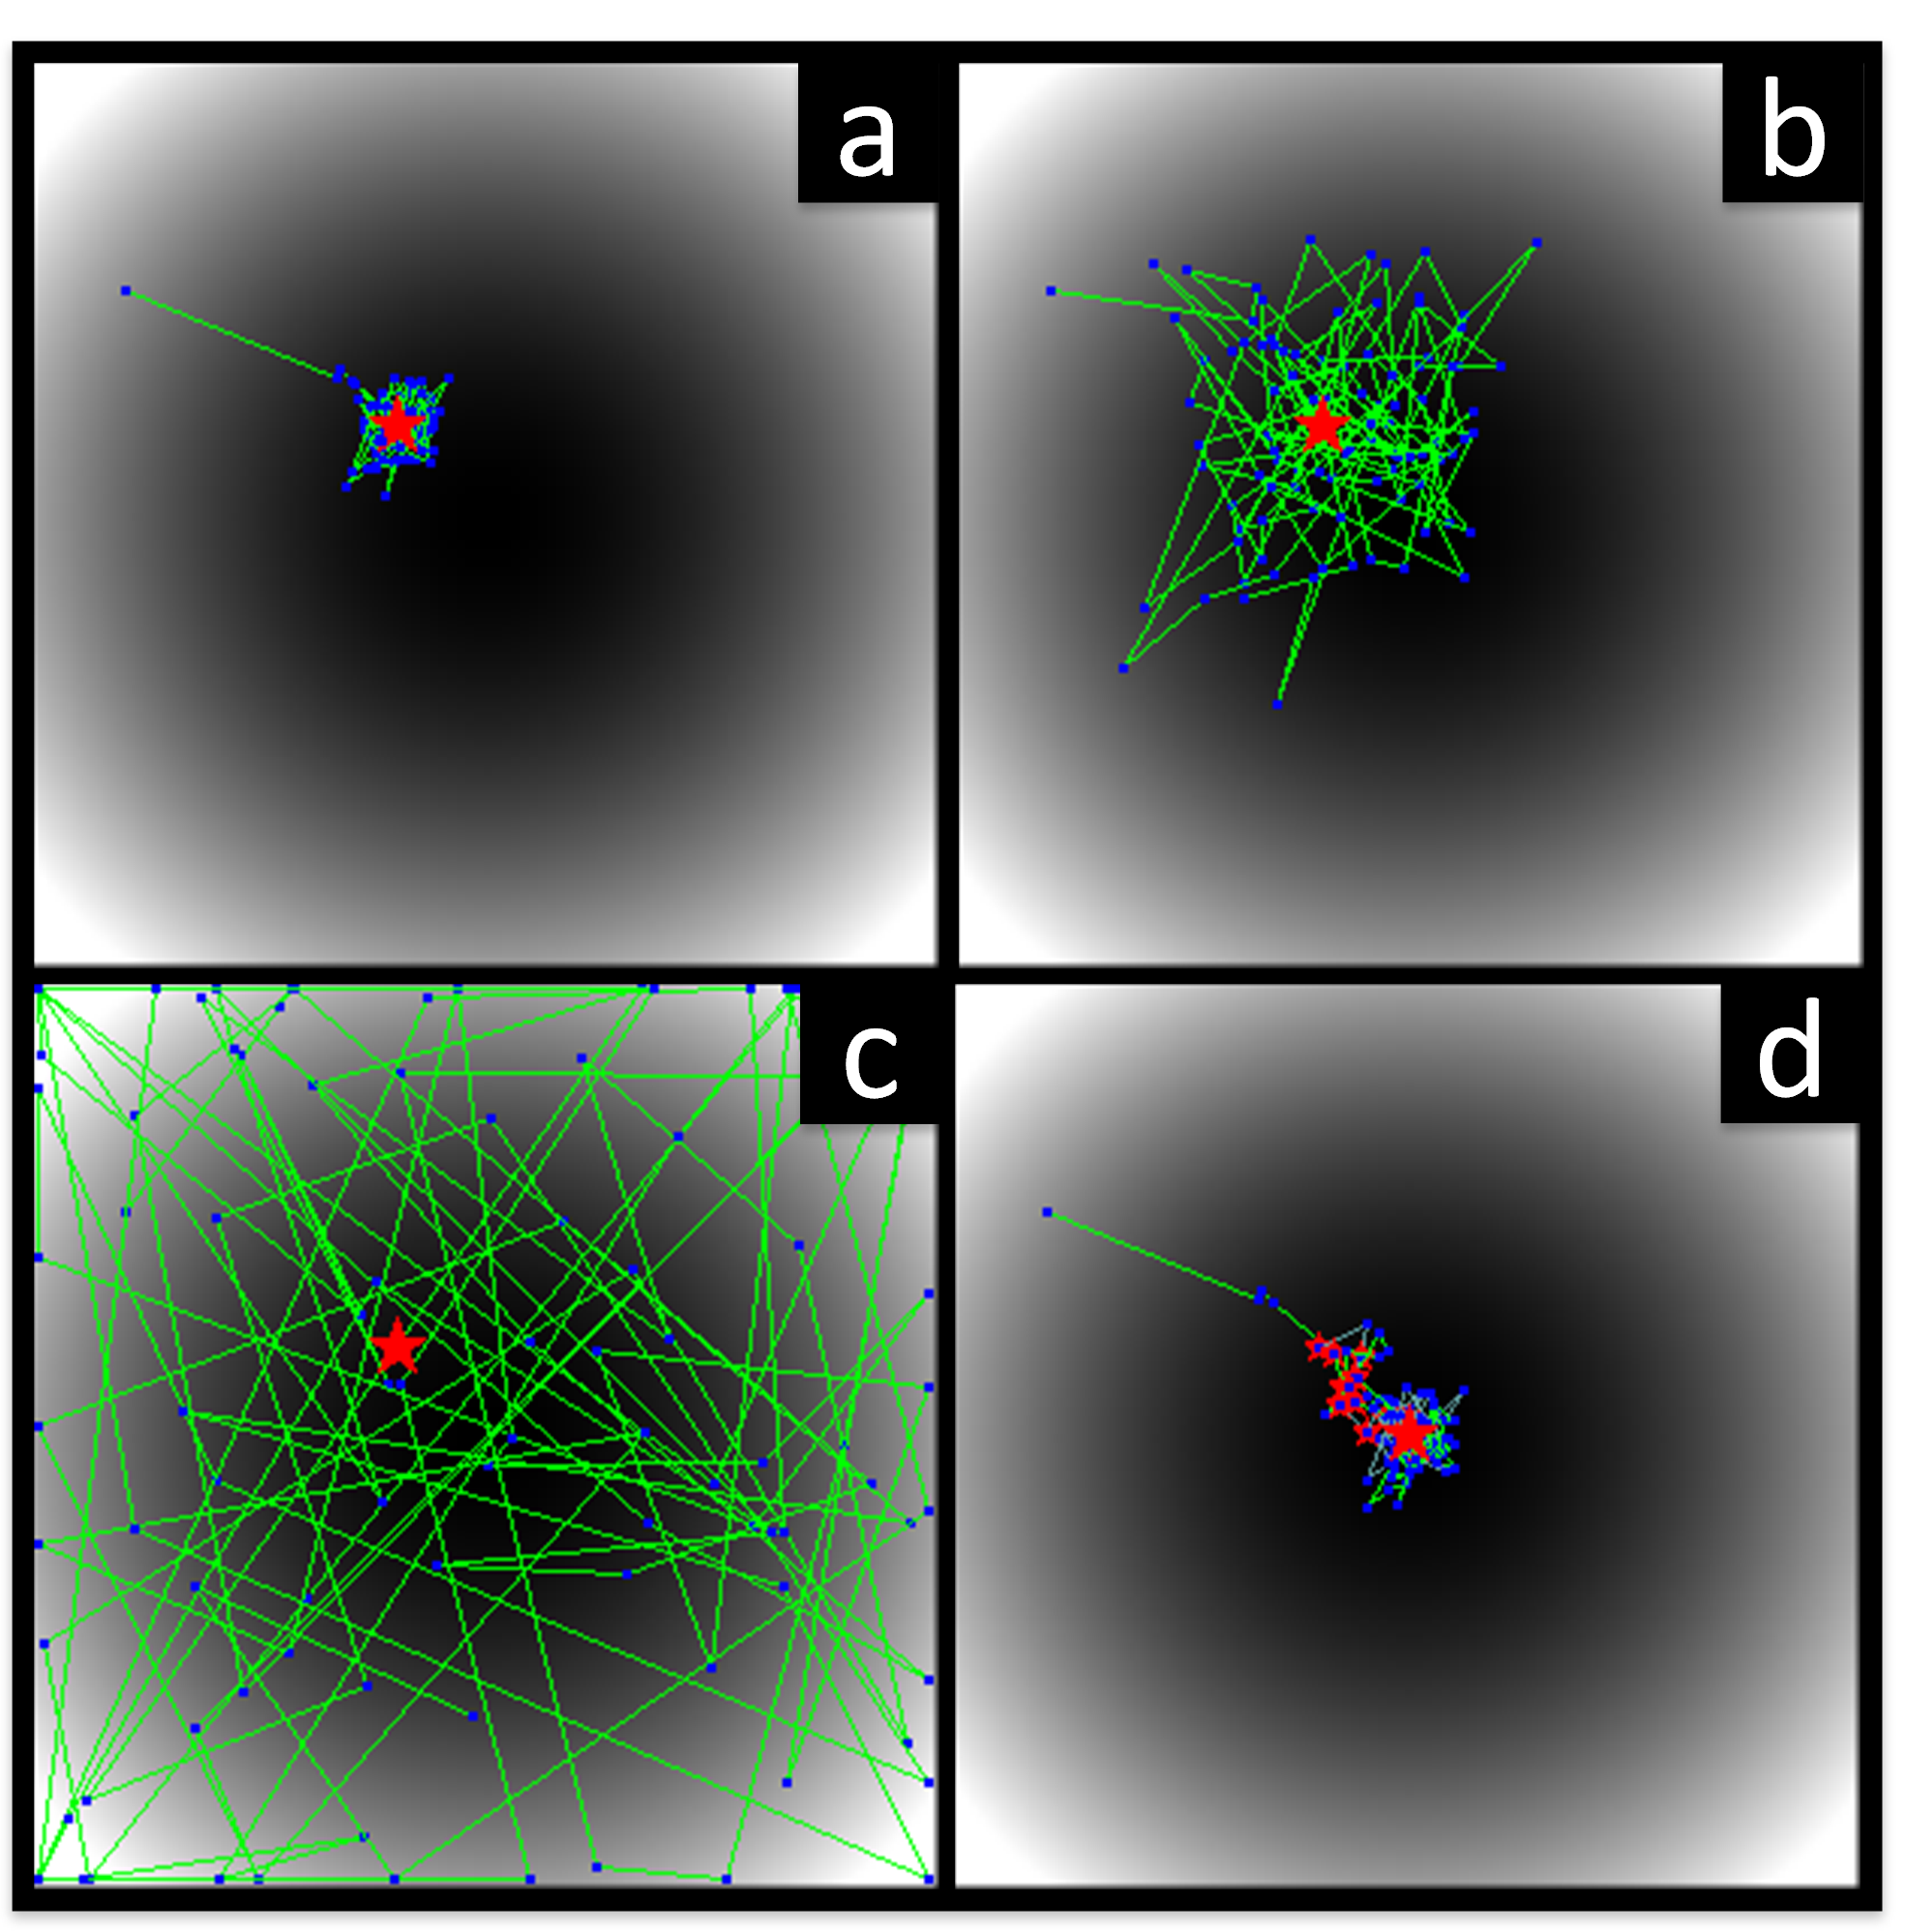
\includegraphics[scale=0.9]{Figuras/Movimento_Original.png}
	\caption{Movimento Original }
	\label{fig:Movimento_Original}
\end{figure}

O item \(d\) da Figura \ref{fig:Movimento_Original} apresenta o resultado do mesmo cenário do item \(a\), porém com a operação de possessão imperial habilitada. Na imagem, as estrelas menores representam os impérios durante as décadas, e a estrela maior representa a posição do império na última década. Observa-se que com a adição do ruído, houveram diversas trocas pelo controle do império entre os países competidores durante as décadas, até a solução convergir para o mínimo global. Outro fato interessante é que neste caso, o valor do ruído levou a um bom tempo de convergência, porém se a operação de possessão imperial tivesse sido habilitada no item \(c\), por exemplo, como mencionado anteriormente, o algoritmo levaria muito mais tempo para encontrar a melhor solução para este problema, pelo fato do ruído estar influenciando demais na definição do passo, que agora passa a ser menos direcionado e mais aleatório. 

A movimentação direta da colônia em direção ao seu país imperialista, isto é, sem adição de ruído, apesar de explorar menos o espaço de busca, converge mais rapidamente para seu império, podendo fornecer uma solução próxima da solução ótima. Por outro lado, quando se adiciona o ruído na movimentação, existe uma maior chance de que a colônia encontre melhores soluções do que a apresentada por seu país imperialista, podendo assim, esta colônia se tornar o centro do império. Esta operação ocorrendo diversas vezes leva os países deste dado império a se moverem para a melhor posição dentro do espaço de busca, de forma que ao fim, ou até mesmo antes do processo evolutivo terminar, se tenha a melhor solução em mãos. Então nota-se uma grande importância na adição de ruído, porém, da forma como é apresentado e calculado, quando um problema apresentar limites de tamanho diferentes, o ruído pode acabar prejudicando a otimização, a velocidade de convergência ou precisão do resultado na busca pela melhor solução.

A partir desta análise, foi possível criar novas formas de movimentação e verificar qual destas seria o melhor modo de mitigar os problemas trazidos com a adição de ruídos na movimentação. Assim foram concebidos os modelos:
\begin{itemize}
\item Movimento Refinado,
\item Visão imperial distorcida e 
\item Combinação de ambos.
\end{itemize}







\subsection{Movimento refinado}
\label{Movimento refinado}

O movimento refinado foi concebido com o intuito de solucionar o problema do movimento Original, o qual tem a geração de ruído fixa, e não proporcional aos limites do problema caso e as dimensões tenham limites diferentes para cada atributo. Então, a proposta é manter o ruído, porém este deve ser proporcional aos limites de cada dimensão. O fluxograma apresentado na Figura \ref{fig:Fluxograms-ColinyEmpireMovement} demonstra a ordem em que ocorrem o cálculo dos valores que irão compor os novos atributos de uma dada colônia para o movimento original descrito anteriormente, sendo o tamanho do passo \(x\) de cada atributo, calculado com o mesmo valor aleatório \(CoefAssimilação\) para todos os atributos, e quando é multiplicado pela distância, se torna proporcional àquele atributo. E antes de atribuir o novo valor a cada atributo, adiciona-se o valor de ruído aleatório. Assim define-se o valor final de cada atributo como apresentado pela equação \ref{eq:ica9}
	
\begin{figure}[hp]
	\centering
	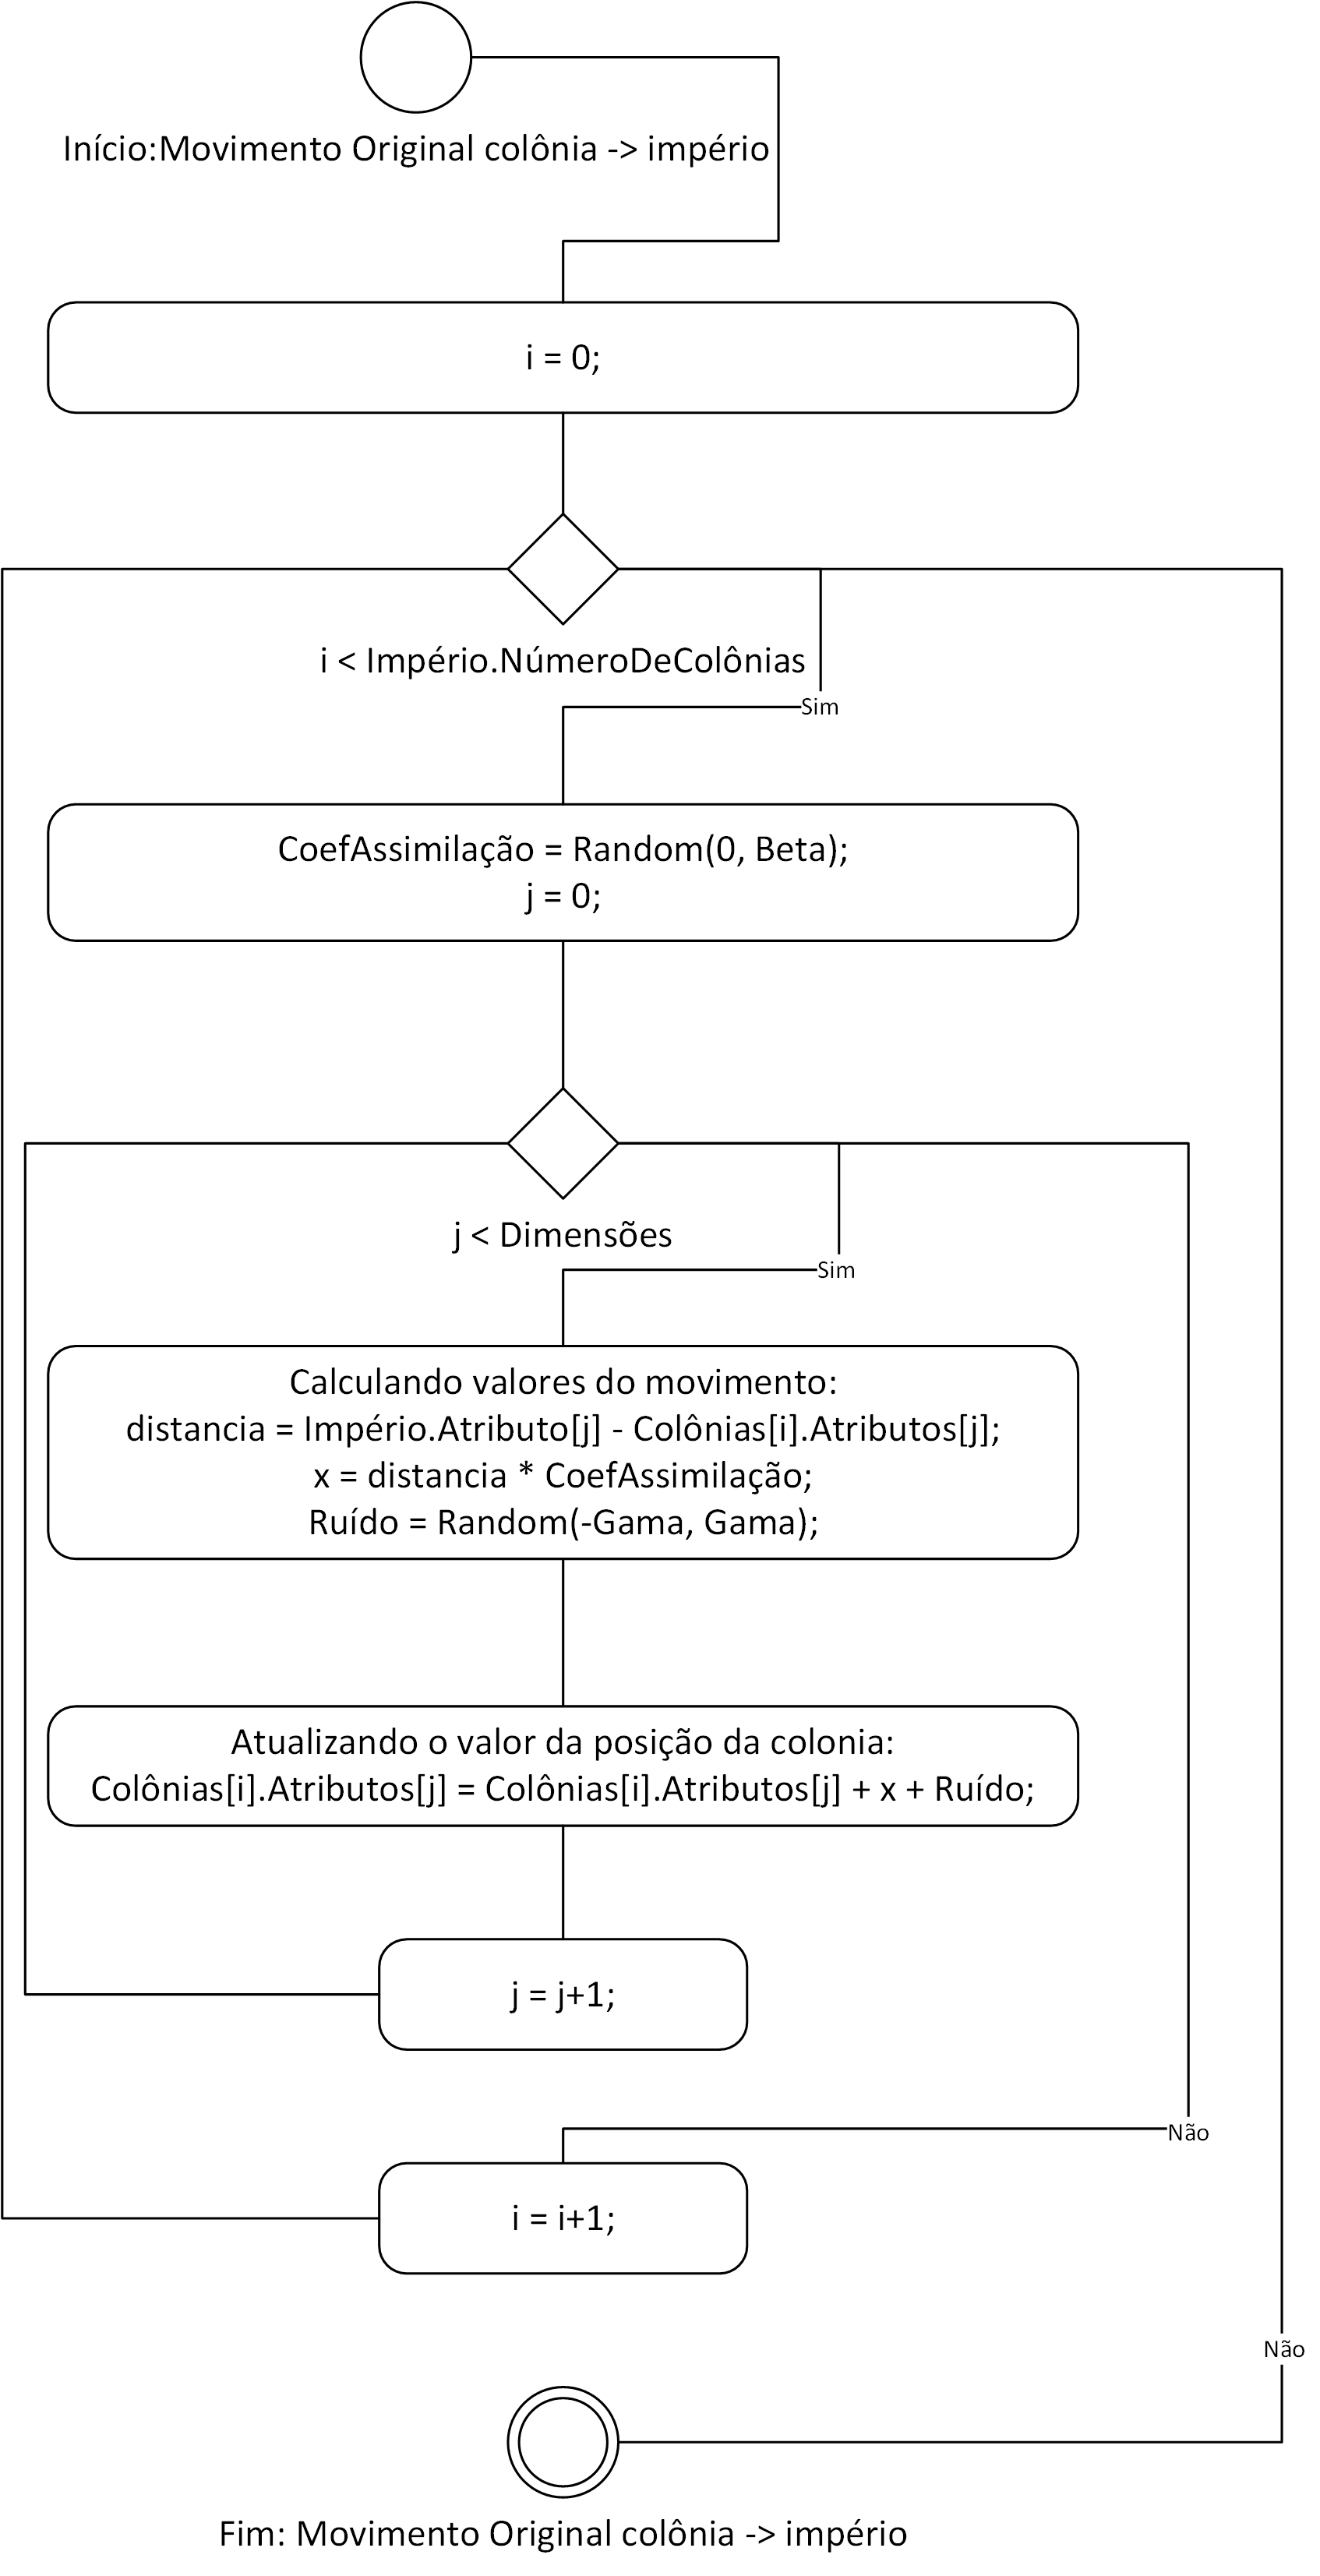
\includegraphics[scale=0.7]{Figuras/Fluxograms-ColinyEmpireMovement.png}
	\caption{Fluxograma Movimento Original ICA }
	\label{fig:Fluxograms-ColinyEmpireMovement}
\end{figure}	

	O método refinado de movimentação então, altera apenas o valor \(\theta\) de ‘Ruído’, que originalmente é calculado como um valor aleatório distribuído normalmente entre o intervalo \(\left[-\gamma, \gamma\right]\), que agora passa a ter uma estrutura dependente dos valores que definem os limites mínimo e máximo para uma dada dimensão e consequentemente do tamanho do espaço de busca, e de um valor de intensidade de ruído, que é um valor de controle, usado para definir o quanto de ruído, proporcionalmente ao espaço de busca, se deseja ter. Assim, este método adiciona uma nova propriedade de controle ao ICA, e troca a equação \ref{eq:ica8} que se resume em:
    
    \[\theta = URand(-\gamma, \gamma);\]
    
pela equação \ref{eq:refined}:

\begin{equation}
\label{eq:refined}
\begin{split}
\theta = 
& TriangularRand(MinBounds[i], MaxBounds[i], dist) \cdot \\ 
& \left(\frac{dist}{TamanhoEspaçoDeBusca[i]} + p \right);
\end{split}
\end{equation}

Sendo a função \(TriangularRand\) uma função que retorna um valor aleatório distribuído triangularmente entre \(MinBounds[i]\) e \(MaxBounds[i]\), e com moda sendo o valor \(dist\) entre o país imperialista e a colônia (observe na Figura \ref{fig:Movimento_Original} que não é apenas usado o valor do módulo da distância, mas sim o vetor distância unidimensional, onde o sinal representará o sentido do vetor). O valor \(p\) é o que define a proporção do ruído, então se \(p\) for definido com o valor de 0.4, o ruído gerado ficará em torno de 40\% do tamanho do espaço de busca de cada dimensão para quando a distância entre o império e a colônia for próxima ou igual a zero. O fator \(\left(\frac{dist}{TamanhoEspaçoDeBusca[i]}\right)\) serve para potencializar o valor de \(p\) quando a distância entre a colônia e o império for grande, porém tende a zero quando o império e a colônia se aproximam, o que anularia o ruído, porém soma-se \(p\) justamente para manter o ruído na proporção desejada.

A função \(TriangularRand\) tem um comportamento muito útil para esta alteração no modo de movimento justamente por gerar os valores, primeiro dentro do intervalo desejado e segundo por gerar tais valores aleatórios tendendo para um valor de moda definido, assim, pode-se gerar valores aleatórios dentro dos limites da dimensão e com a moda sendo a distância entre a colônia e o país imperialista, o que implica que a maior parte do ruído é gerado com mais chances de estar mais próximo ao império, aumentando a velocidade de convergência ao mesmo tempo que mantém uma pequena chance de ruídos mais intensos. A Figura \ref{fig:RandomTriangular-White} abaixo representa um histograma de três sequências de 1000 valores gerados por esta função no intervalo \(\left[0,1\right]\) e de moda 0, 0.5 e 1 respectivamente. Observa-se então, que existirá uma chance muito maior de que os valores aleatórios gerados pelo ruído estejam mais próximos da distância percorrida, mantendo uma forma de controle sobre o ruído gerado e no caso, quanto mais a distância diminui menor também será a chance de existirem ruídos mais intensos. 
	
Apenas com o uso da função que gera valores aleatórios de distribuição triangular, já adiciona uma forma de ruído proporcional ao espaço de busca, porém ela ainda gera valores que podem levar a colônia para qualquer posição do espaço de busca aleatoriamente, quando a colônia estiver muito distante do império, fazendo com que a otimização fique muito mais aleatória do que direcionada. Então definiu-se \(p\) como sendo um valor definido dentro do intervalo \(\left[0,1\right]\) o qual soma-se com o valor proporcional da distância em relação ao espaço de busca \(\left(\frac{dist}{TamanhoEspaçoDeBusca[i]}\right)\), que então multiplica o valor gerado aleatoriamente com distribuição triangular entre os limites da dimensão e com moda como sendo a distância entre o atributo da colônia e do império nesta mesma dimensão, tornando este ruído limitado proporcionalmente a uma porção do espaço de busca. 
    
\begin{figure}[H]
	\centering
	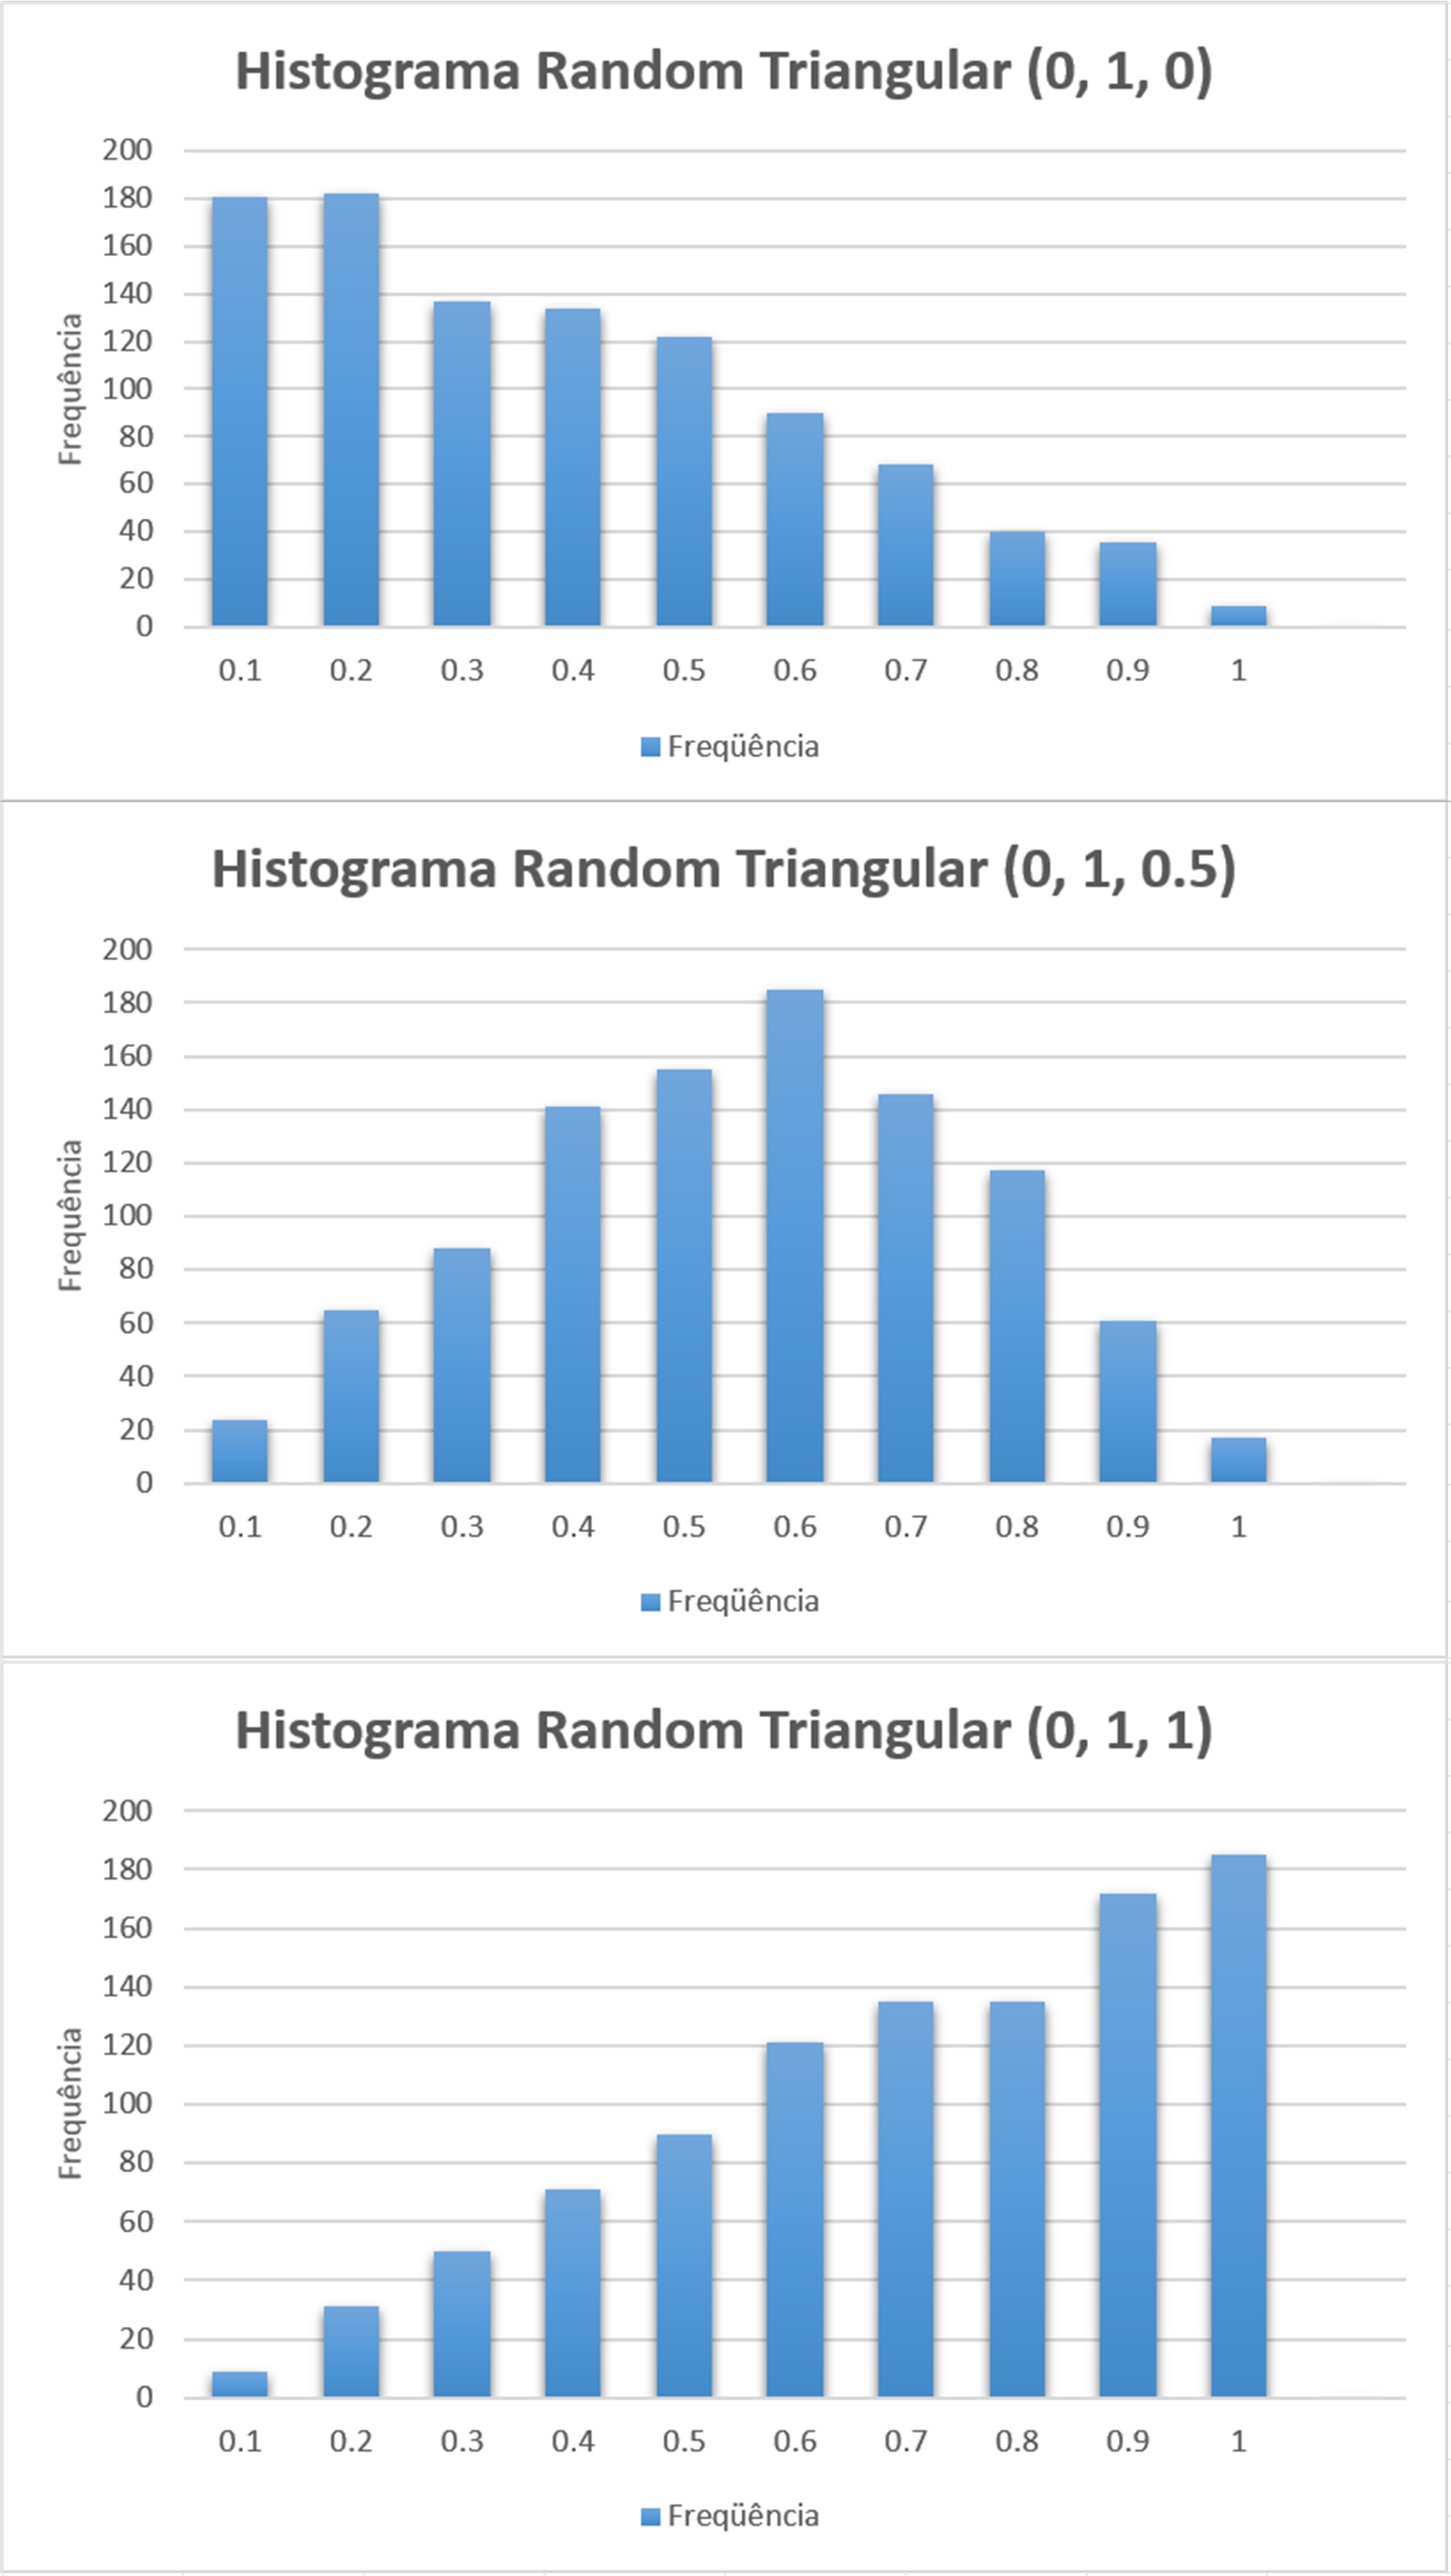
\includegraphics[scale=0.55]{Figuras/RandomTriangular-White.png}
	\caption{Random Triangular}
	\label{fig:RandomTriangular-White}
\end{figure}

A Figura\ref{fig:Movimento_Refinado}, analogamente a Figura \ref{fig:Movimento_Original}  apresenta 4 configurações diferentes para a busca da melhor solução, na qual as três primeiras são com a operação de possessão imperial desabilitada e a última tem esta funcionalidade habilitada. Observa-se que as imagens são muito parecidas, portanto agora existe um controle muito mais preciso sobre a intensidade  do ruído a ser gerado, sendo que os valores para p foram de 0.1, 0.4 e 0.8 para os resultados \(a\), \(b\) e \(c\) respectivamente, e em \(d\) foi utilizado p = 0.1 e a operação de possessão imperial estava habilitada. Em comparação com o modelo original, ao utilizar o método refinado, ocorrem aproximadamente 10\% mais possessões imperiais, ou seja, aumentaram-se as chances de uma colônia se mover para uma posição melhor que a de seu país imperialista em 10\% durante esta etapa de movimentação, uma vez que agora existe uma heurística mais bem definida em relação à adição de ruídos e à intensidade destes.

\begin{figure}[htp]
	\centering
	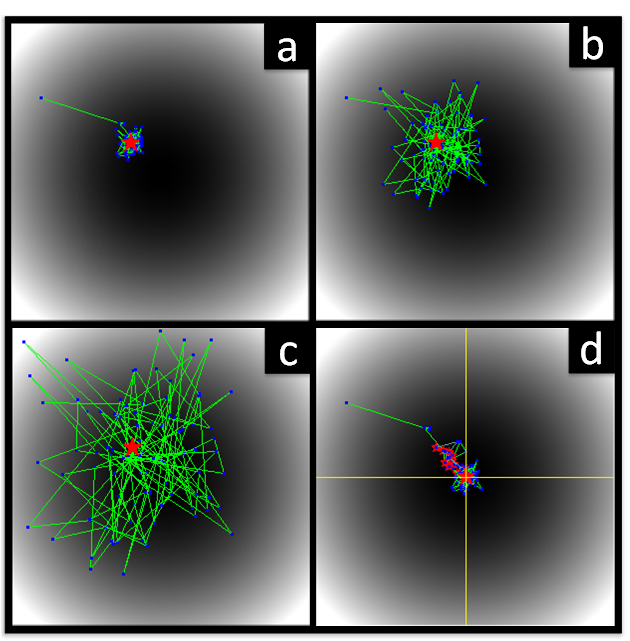
\includegraphics[scale=0.9]{Figuras/Movimento_Refinado.png}
	\caption{Testes com movimento refinado}
	\label{fig:Movimento_Refinado}
\end{figure}






\subsection{Visão imperial distorcida}
\label{Visão imperial distorcida}


A movimentação de uma colônia em direção ao seu país imperialista nada mais é que a tendência da colônia  se parecer mais com seu império ao longo do passar de décadas. Para que a colônia se molde de forma a ter suas características mais parecidas com a de seu império, ela primeiro calcula o quão distante suas características estão do seu império, e então se movimenta em direção ao seu imperialista de acordo com um valor de assimilação. 

Quando uma colônia observa as características de seu império, para então calcular a distância entre cada característica, existe a possibilidade de que esta colônia não localize muito bem a posição ou valor exato da característica do seu império, de modo que tal distorção seja influenciada pelas posições das demais colônias do império. Assim, quando a colônia calcula o quão distante suas características estão de seu império, ela também observa quais são as características mais distantes ao imperialista, dentre todas as colônias, e adiciona um valor aleatório, distribuído normalmente, na característica do império, para então calcular uma distância com uma visão distorcida destas características do império.

Esta distorção é uma adição de ruído proporcional não ao espaço de busca em geral, mas sim em relação ao posicionamento de todas as colônias do império, isto é, em relação a área ou região do espaço de busca ocupada pelo império. Este tipo de ruído é uma otimização que faz com que a solução seja explorada localmente tal que a melhor solução seja encontrada mais devagar, porém explora localmente de forma aleatória o caminho a ser feito pela colônia, até que esta chegue ao país imperialista. Quanto mais próximas o grupo de colônias estiver de seu império, menor será a região ocupada pelo império e menor também será o ruído gerado. O ruído se torna nulo quando as colônias compartilharem as mesmas posições com seu império. Para se conhecer esta região do império, basta obter as distâncias máximas entre as colônias e o império, isto é, obtém-se os limites do império através das características mais distantes das colônias. Estes valores são armazenados localmente em um vetor \(maxDists\), que é gerado segundo o Algoritmo \ref{alg:CalculoMaxDists}
    
\vspace{10px}
\begin{algorithm}[h]
\SetAlgoLined
\KwData{
\\ Império - o império em questão.
\\ Colônias - o vetor de colônias.
\\ Dimensions - o valor que representa a quantidade de dimensões do problema.}
\KwResult{ 
\\maxDist - o vetor de distâncias máximas de cada atributo entre o império e todas as suas colônias.
}
maxDist = new Double[Dimensions]\;

\For{$i \leftarrow $0 \KwTo $Dimensions$}
{
	\For{$j \leftarrow $0 \KwTo $Império.NumColônias$}
    {
    	localDist = ABS(Império.Attributes[i] - Colônias[j].Attributes[i])\;
        maxDists[i] = MAX(localDist, MaxDist[i])\;
    }
}
\caption{ Cálculo das distâncias máximas para Visão Imperial Distorcida.}
\label{alg:CalculoMaxDists}
\end{algorithm}

Assim utiliza-se o vetor \(maxDists\) multiplicado de um valor aleatório distribuído normalmente e soma-o na posição do império, e então subtrai-se o valor da posição da colônia, para se obter o valor de distância distorcido, como mostra a equação \ref{eq:CalcVIDDist}:

\begin{equation}
\label{eq:CalcVIDDist}
\begin{split}
dist = 
&(Império.Attributes[i] + GausRand() \cdot maxDists[i]) - \\ &Colônia.Attributes[i]
\end{split}
\end{equation}

Após o cálculo da distância distorcida, o algoritmo da movimentação prossegue normalmente no seu fluxo como algo semelhante ao fluxo apresentado pela Figura \ref{fig:Movimento_Original}, que será então multiplicada pelo coeficiente de assimilação e atribuída ao valor do atributo (ou característica), com a exceção de que agora não se calcula e nem se adiciona o ruído provido pelo valor aleatório baseado em \(\gamma\). 

Este método de adição de ruído é proporcional à distância entre a colônia e império, isto quer dizer que apenas quando o módulo da distância entre ambos for maior que zero é que existirá ruído. Assim quando a colônia se posicionar junto de seu império, não existirá alteração nenhuma na posição da colônia durante a etapa de movimento provinda do ruído. Ao comparar apenas uma colônia com um império, pode-se obter resultados que não sejam ótimos, porém esta alteração funciona muito bem com impérios que possuem várias colônias, uma vez que com muitas colônias tem-se uma exploração maior da região e a tendência será a de tornar o país menos custoso como sendo o centro do império utilizando a operação de possessão imperial.


A Figura \ref{fig:Testes_Vis_o_Imperial_Distorcida} mostra em \(a\) o caso de um país imperialista e uma colônia, com a operação de possessão imperial desativada. Observa-se que quanto mais próxima a colônia está do império, menos desvio ocorre em seu movimento. Em \(b\) tem-se o mesmo caso de \(a\) porém com a competição imperialista habilitada. Neste caso, existem algumas trocas entre império e colônia, porém a conversão para a melhor posição não ocorre. O item \(c\) representa uma configuração diferente, com 1 império e 9 colônias, totalizando 10 países, assim percebe-se como este tipo de movimento é sempre direcionado para o império, e ainda possui uma variação no movimento que decai à medida que a colônia chega perto do império. Por fim \(d\) é uma combinação de imagens que representam o cenário do item \(c\) durante as décadas de 1 a 5.

\begin{figure}[h]
	\centering
	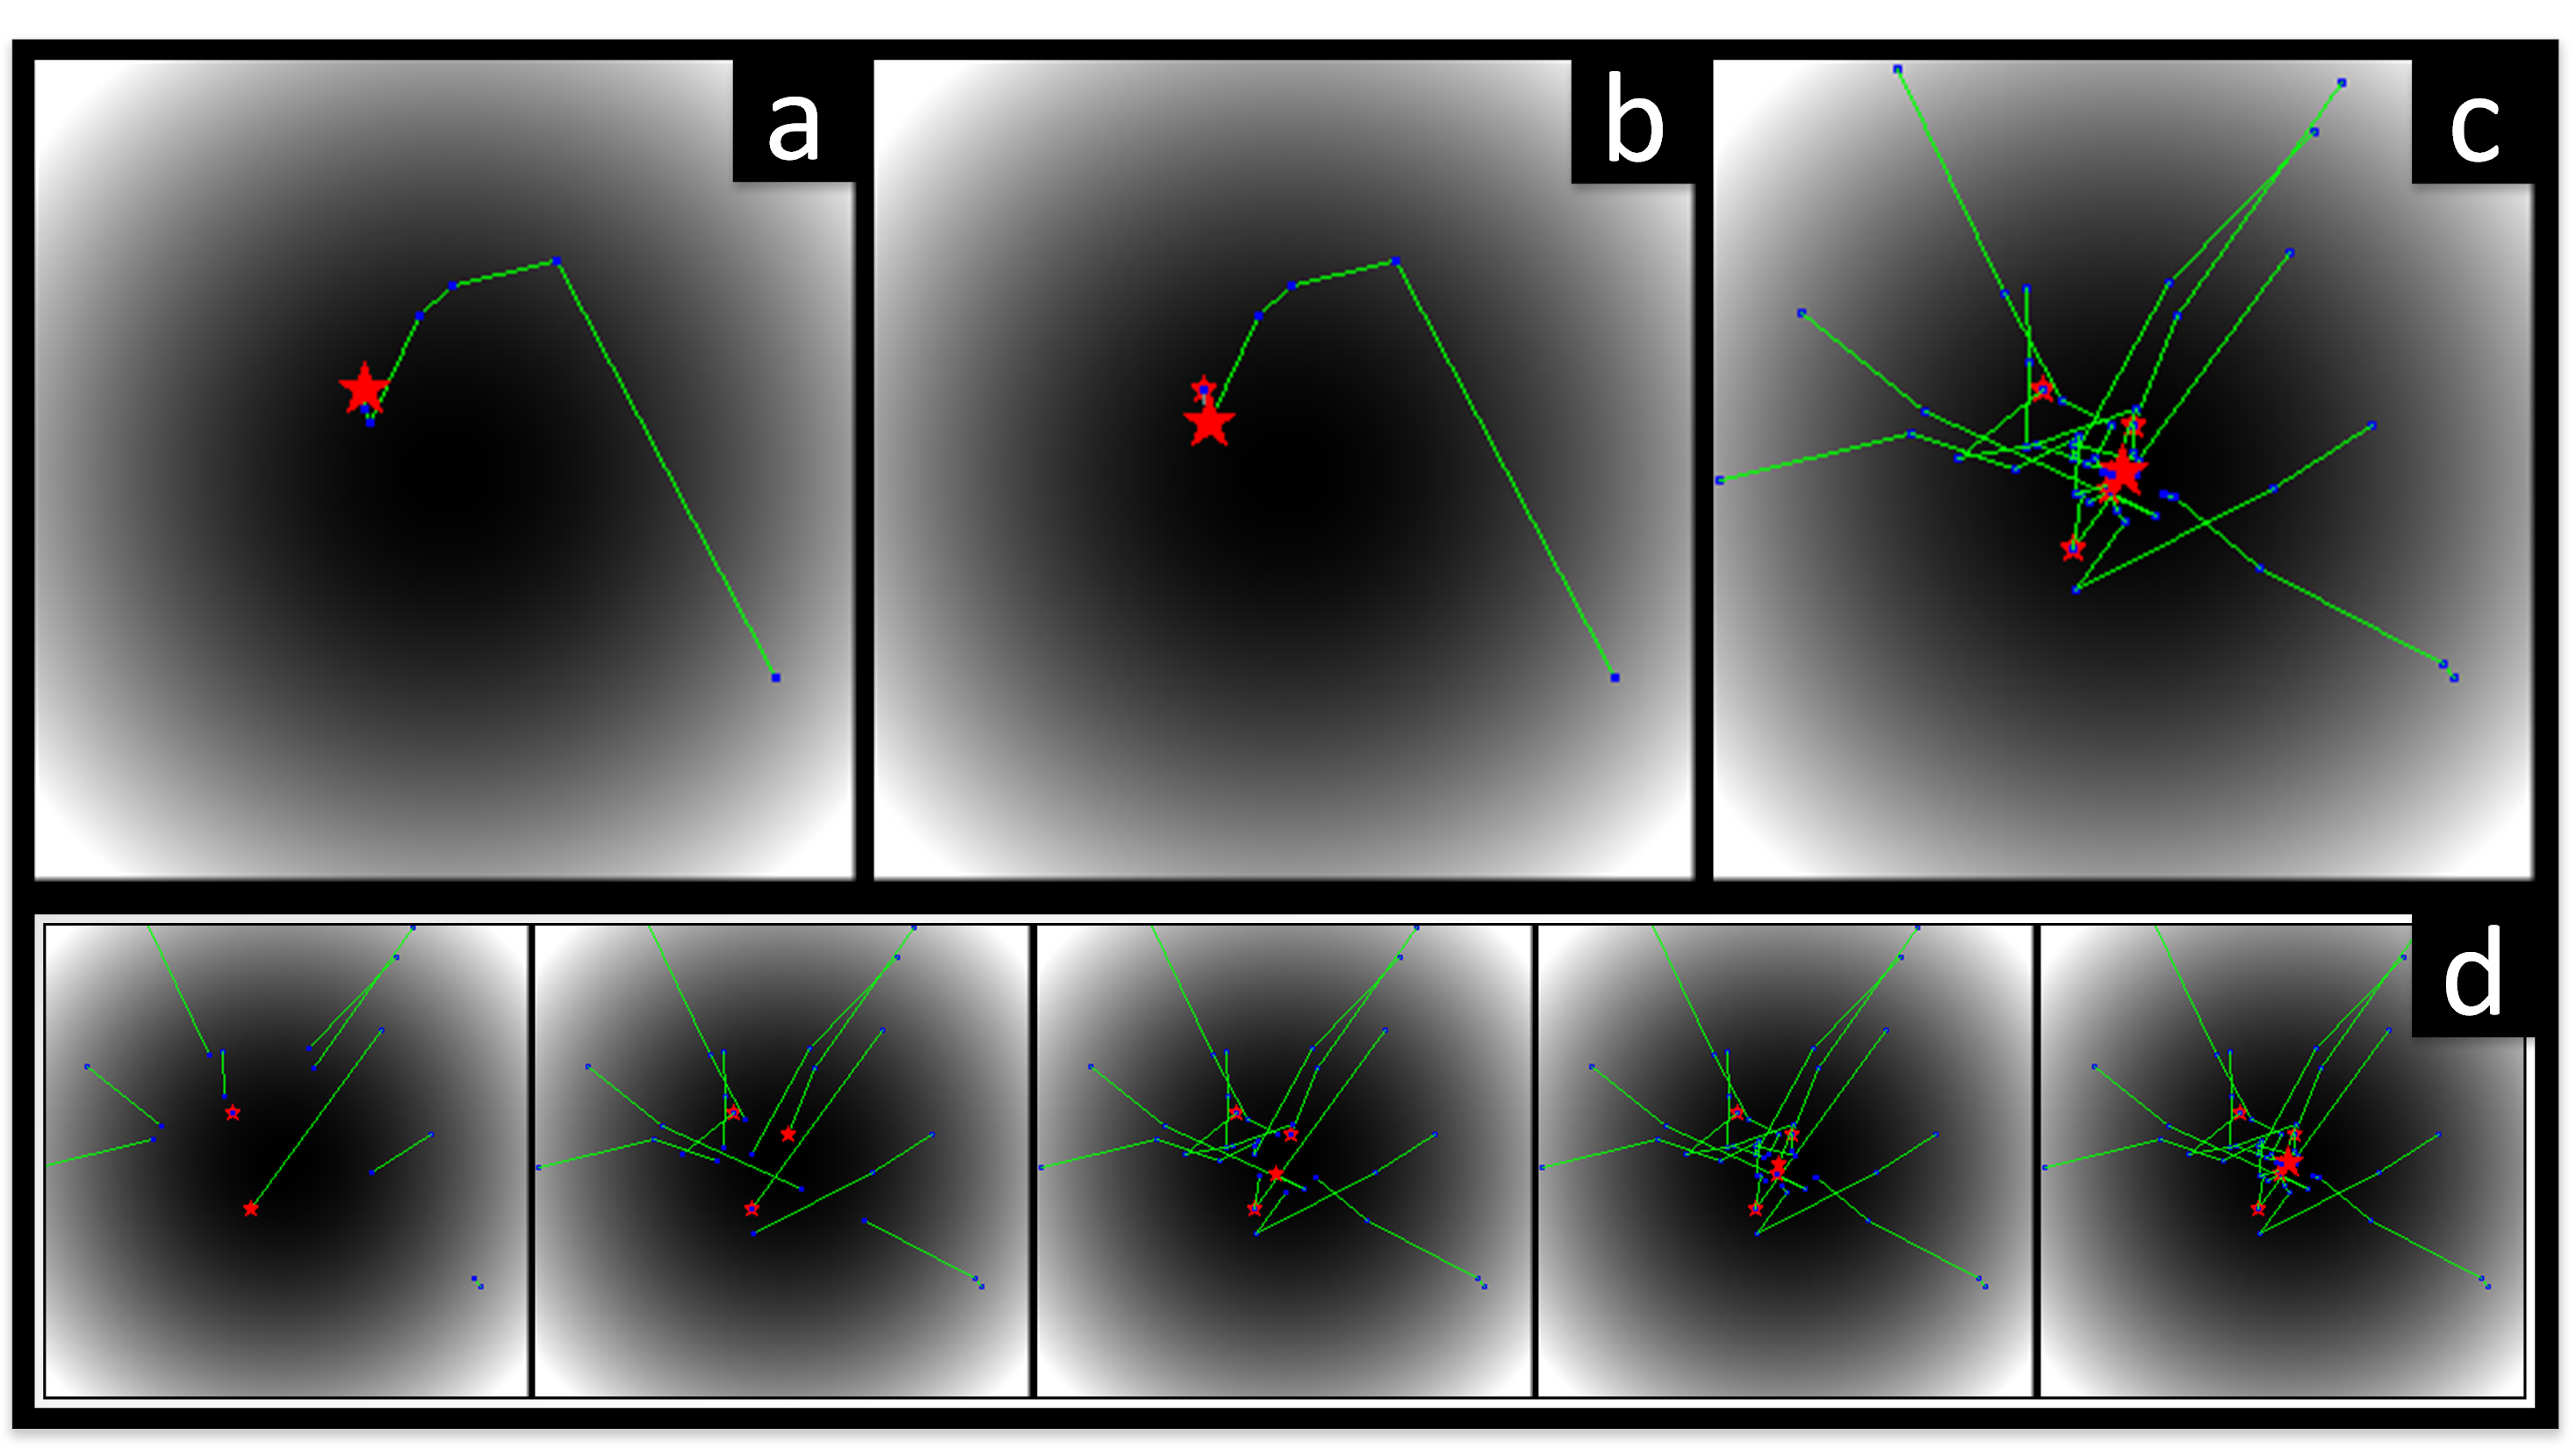
\includegraphics[scale=0.6]{Figuras/Testes_Vis_o_Imperial_Distorcida.png}
	\caption{Testes Visão Distorcida}
	\label{fig:Testes_Vis_o_Imperial_Distorcida}
\end{figure}

Comparando então ambas as alterações, com o método refinado de movimentação, é possível controlar o ruído proporcionalmente ao espaço de busca, mesmo que suas dimensões estejam limitadas em valores e escalas completamente diferentes, possibilitando que um país tenha seu vetor de atributos composto por muito mais elementos sem que o ruído seja um fator que atrapalhe a evolução da solução. Um ponto interessante para se analisar é a quantidade de ruído em relação a precisão da busca pela solução, de modo que tem-se como objetivo principal da movimentação, apenas a transição das características de um indivíduo até as características de seu império, pois o algoritmo possui outros recursos, como o aumento do número de países e impérios, operação de revolução imperialista, e até mesmo a competição imperialista em si, fazem com que a adição de ruído pareça redundante. Porém, este não é o caso, o ruído quando usado em uma porcentagem baixa e durante a movimentação, melhora a busca pela melhor solução localmente, fazendo com que o império se mova para o vale (ou pico) local mais rapidamente (a movimentação de um império ocorre quando há troca  entre império e colônia, através da operação de possessão imperial). E por fim, como mencionado anteriormente, os demais métodos tem o objetivo de evitar que a solução fique estagnada em mínimos (ou máximos) locais, uma vez que possuem apenas o fator aleatório e não são direcionadas, como a movimentação. 

Já o método de movimentação por visão imperial distorcida tem como intuito apenas inserir ruído que seja proporcional às colônias mais distantes do império, trazendo a ideia de que quanto mais distante uma colônia está de seu império mais míope ela é para definir as características de seu império. Assim a exploração do espaço de busca não formará caminhos em linha reta, mas sim caminhos que sejam aleatórios até que a colônia de fato chegue ao império. Esta forma aleatória de se mover pode aumentar o tempo que uma colônia leva para chegar até seu imperialista e lá ficar estagnada, mas por outro lado aumenta a chance do império sair de mínimos (máximos) locais se deslocando pelas décadas através da operação de possessão imperial.

Ambos os métodos ainda possuem um mecanismo de ‘freio’, geralmente relativo ao número máximo de décadas, usado para decrementar gradualmente a quantidade de ruído gerada durante as décadas até que esta quantidade de ruído seja anulada ou se mantenha fixa em um valor. Assim como o decrescimento da operação de revolução colonial decresce, a quantidade de ruído também decresce, porém existe a possibilidade de manter este ruído até o fim (até que uma condição de parada seja atingida), ou também existe a possibilidade de controlar o decrescimento para que os ruídos sejam decrementados até se anularem durante o processo evolutivo. Quando os ruídos tendem a se anular, a forma de movimento tende ao método de movimento linear, que por sua vez é mais rápido e leva à conversão ideal (onde os países estejam na mesma posição de seu imperialista). Desta forma, pode-se ter uma quantidade grande de ruído nas primeiras décadas, de modo a explorar melhor o espaço de busca, evitando mínimos locais, e gradualmente diminuir o ruído para ajustar a posição do império para a melhor possível e por fim, anular os ruídos para que o processo evolutivo possa convergir para o cenário ideal.

A combinação de ambos os métodos mantém a velocidade de deslocamento do império durante as décadas constante, porém mantém o ruído gerado pela visão imperial distorcida sempre ativo nas colônias que sofreram deslocamento por ruído refinado na década passada, isto é, o ruído gerado pelo método refinado faz com que algumas colônias sempre estejam fora do centro do império e limitados em uma região proporcional ao espaço de busca, então, na próxima década, será aplicado a elas, o ruído gerado pela visão imperial distorcida (pois ele é usado quando se calcula a distância, antes de se aplicar o ruído gerado pelo método de movimento refinado), assim este ruído gerado pela visão imperial distorcida será constante e limitado no espaço definido pelo método de movimento refinado, e como ele é proporcional distância entre colônia e império, também passa a ser proporcional ao limite definido no ruído gerado no movimento refinado. A Figura \ref{fig:MovimentoCombinado} mostra a evolução durante as décadas 1, 4 e 8 respectivamente nos itens \(a\), \(b\) e \(c\).

\begin{figure}[h]
	\centering
	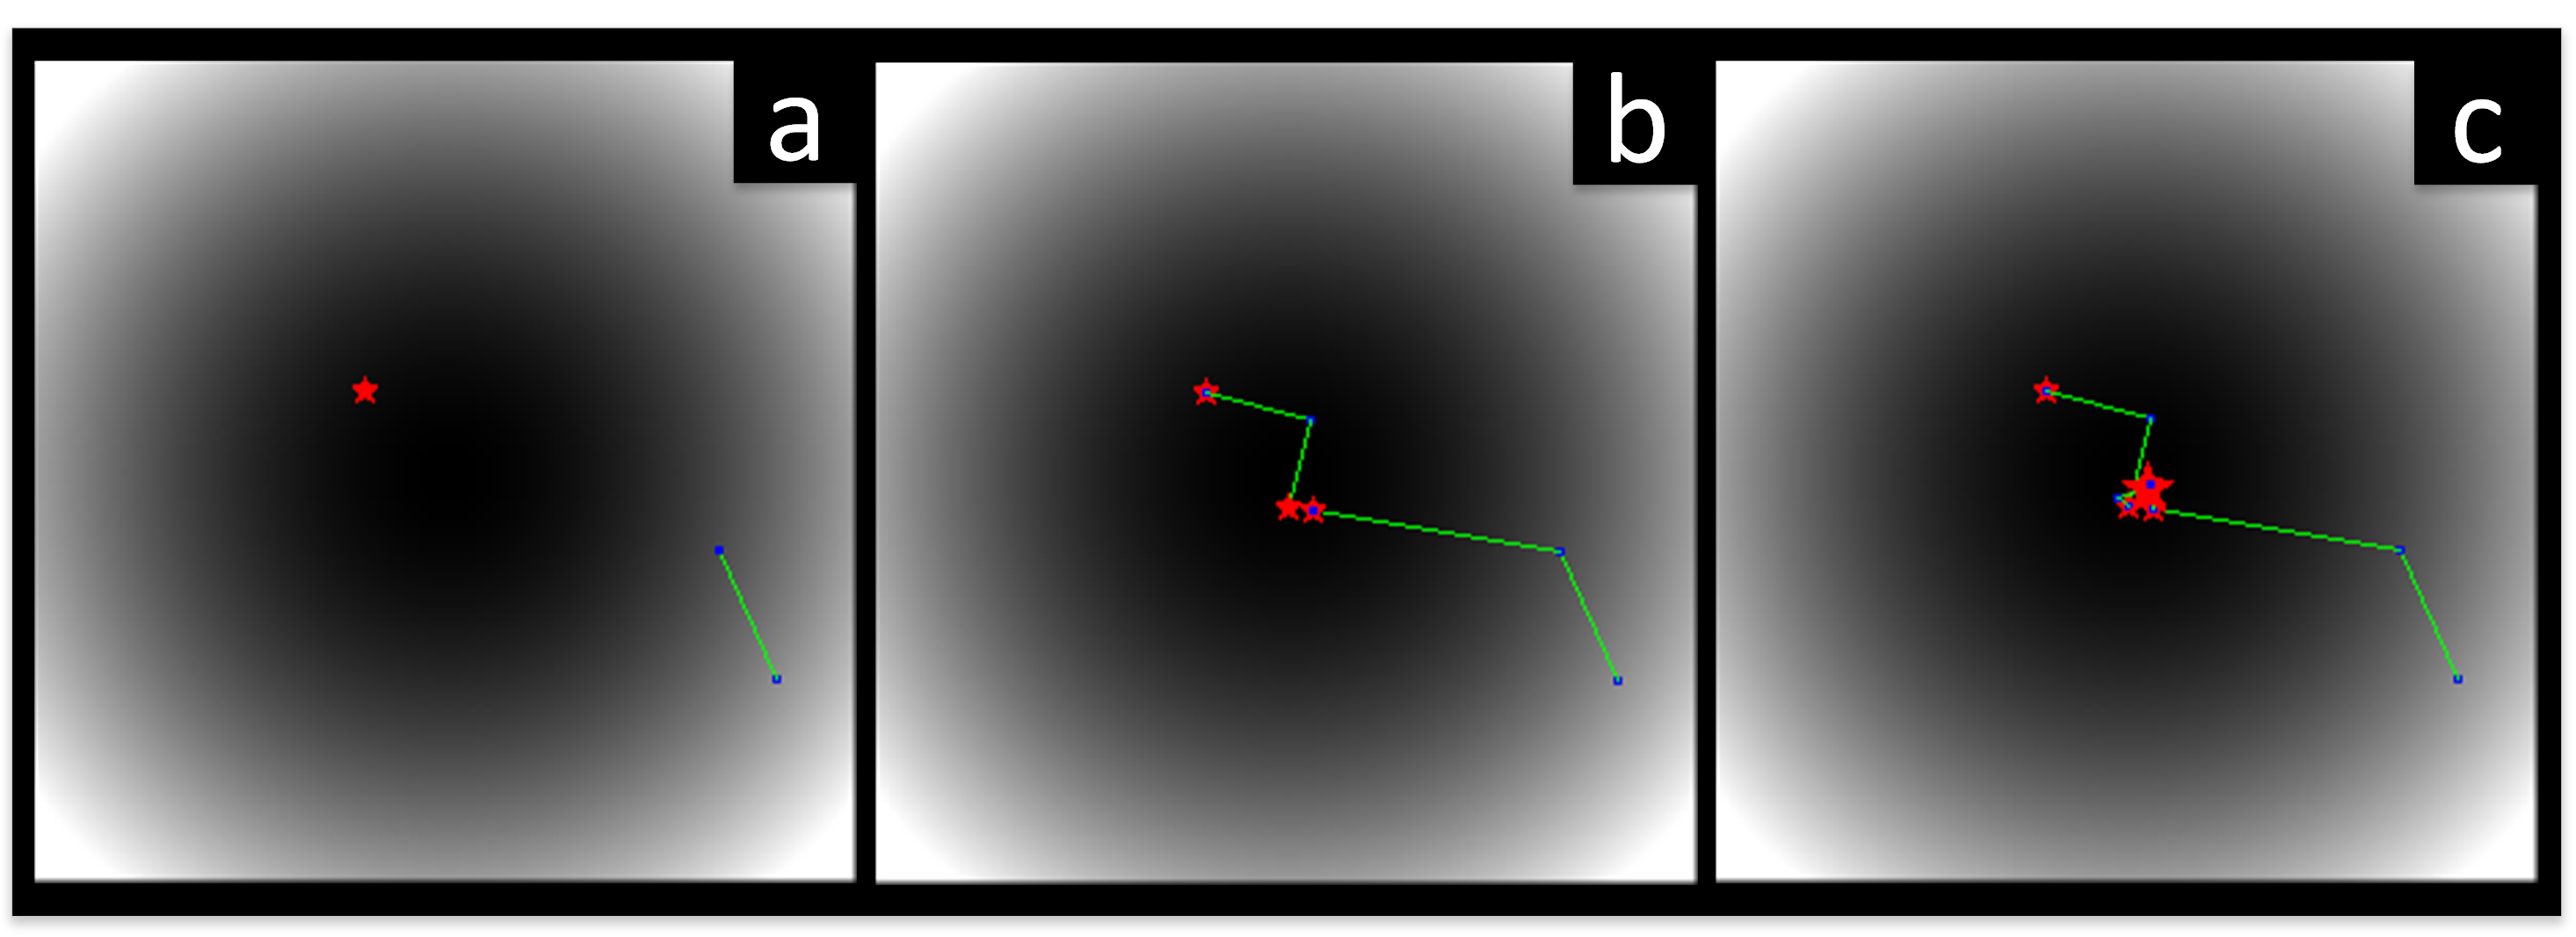
\includegraphics[scale=0.6]{Figuras/MovimentoCombinado.png}
	\caption{Movimento combinado}	
    \label{fig:MovimentoCombinado}
\end{figure}

Concluindo esta seção, tem-se agora três (Refinado, Visão imperial distorcida e Combinado) métodos capazes de mover os países, inserindo ruídos proporcionais ao espaço de busca de forma controlada e que ainda é capaz de atingir o cenário ideal de convergência, diferentemente do modelo proposto por \citeauthor{atashpaz2007imperialist} em \cite{atashpaz2007imperialist} e \citeauthor{roche2011imperialist} em \cite{roche2011imperialist}, ao adicionar o ruído fixo, o qual levaria a impossibilidade de convergência para o cenário ideal. O método combinado pode apresentar soluções melhores, mas em contrapartida são necessários mais cálculos e consequentemente mais processamento. Caso a função de aptidão(\emph{Fitness}) seja de rápida avaliação, é ideal usar o modelo refinado, para ruídos independentes da distância entre colônia e império, ou o método de visão distorcida, para ruídos dependentes da distância. já em casos onde o problema apresenta alto custo computacional, o cálculo da forma de movimento não será tão impactante, porém aconselha-se fazer com que os ruídos cessem após uma quantidade de décadas para que a solução possa convergir para o cenário ideal, encontrando o ponto ótimo entre o quanto se deve explorar o espaço de busca de forma mais aleatória e o quão rápido se deve convergir. 






\section{Paralelização do ICA}
\label{Paralelização do ICA}


Algoritmos evolutivos têm como parte essencial para convergência a função de aptidão, que deve ser bem definida e voltada para o problema. Tal função, deve ser executada durante todas as décadas. No ICA, a função de aptidão proposta foi definida de forma a executar cálculos os quais resultam em um valor de custo para o país, tal que este custo seja utilizado por todos os componentes do ICA, a fim de buscar pela melhor solução. A quantidade de chamadas à função de aptidão é dependente basicamente de dois valores, do número de países \(np\) e número de décadas \(nd\). 


Sabendo que os países sempre são avaliados, todos de uma só vez, e que em cada década todos os países devem ter seu valor de custo calculado, pode-se dizer que em cada década seus atributos se modificam de acordo com a posição de seus impérios. E ainda, leva-se em conta que inicialmente todos os países são avaliados e têm seus custos atribuídos, antes mesmo da separação entre colônias e impérios. Desta forma, é possível calcular a quantidade total de chamadas da função de aptidão durante uma execução completa do ICA como a expressão \ref{eq:quantidade de chamadas fitness}:


%\[
\begin{equation}
\label{eq:quantidade de chamadas fitness}
np \times (nd + 1)
\end{equation}
%\]


Dependendo do tipo de problema, algoritmos evolutivos podem levar diversas épocas, no caso do ICA, décadas, para convergir em uma solução dentro dos critérios de parada (que foram definidas no capítulo x). Em casos cujo problema se expande para o domínio não linear existe a possibilidade de executar tais operações muito mais vezes do que o esperado para se chegar ao resultado. 


No problema a ser solucionado por este trabalho, a função de aptidão utilizará muito processamento para o cálculo de custo de cada país. Para que tal solução possa ser executada diversas vezes, em tempo hábil, e também de forma que o problema possa ser testado dentro de diferentes abordagens, é necessário utilizar todos os recursos tecnológicos disponíveis. 


Para otimizar a velocidade com que o ICA faça tais cálculos, foi desenvolvida uma adaptação na parte central do ICA, de forma que as chamadas para avaliação das funções de custo dos países sejam executadas paralelamente, já que o cálculo de custo do país são independentes dos demais indivíduos, usando todos os núcleos de processamento possíveis. Assim, a aplicação tem um ganho significativo de tempo e um aumento significativo de processamento, que depende de quantos núcleos estão disponíveis para a execução do ICA


Um fato técnico interessante, é que para se utilizar de forma ótima toda esta alocação de núcleos de processamento, devemos levar em conta que o número de indivíduos deve ser múltiplo do número de núcleos de processamento para que todos sejam utilizados com capacidade máxima para o processamento da função de aptidão. Caso este número seja diferente, também haverá uma melhora, porém um dos núcleos poderá ficar ocioso durante os cálculos, fazendo com que indiretamente se “perca” a capacidade total de processamento em um ou mais núcleos. Tal perda de capacidade de processamento pode ser devido também à alocação de processamento pelo sistema operacional para um processo concorrente, porém caso exista apenas o processo em questão, ou caso tenha alta prioridade, deve-se considerar a utilização de número de países múltiplos do número de núcleos.


A paralelização dos cálculos de custos dos países foi implementada de modo a ser opcional. Por padrão já está ativa, porém ao se configurar os dados iniciais para a solução de um dado problema, fica a critério do desenvolvedor, decidir se utilizará ou não o algoritmo de forma paralelizada.


Algo que pode ser chamado de desvantagem em se paralelizar esta parte do algoritmo, aplica-se apenas no momento em que é necessário executar uma depuração no código que faz o cálculo do custo do país. O que ocorre no caso normal, não paralelo, é que para se depurar uma função, se escolhe uma parte do código, a qual se deseja depurar e então a execução do programa sofrerá uma pausa quando chegar naquele ponto. Quando se utiliza a técnica de paralelização para executar as funções (neste caso as funções são as mesmas, porém apenas a chamada da função é alterada), cada núcleo disponível irá alocar uma tarefa (thread) para executar as funções em paralelo, assim, como foi definido um ponto de depuração dentro da função, toda vez que uma das tarefas atingir o ponto de depuração, ela irá pausar a execução do programa, apresentando os valores a serem depurados para o seu contexto de execução da tarefa, e impedindo que uma depuração por passos possa ser feita sequencialmente apenas em uma tarefa sem que um filtro seja criado em tempo de execução. Tal filtro de depuração para pontos de parada só podem ser adicionados em tempo de execução porque inicialmente não se sabe qual será a identificação da tarefa que irá rodar em paralelo por ela não ter sido criada ainda. É importante fixar que a depuração não é impedida ou resulta em erros, mas tal desvantagem se dá na adição de passos para filtrar e isolar a depuração para apenas uma tarefa.


A melhora no desempenho não é apenas dependente da paralelização do cálculo dos custos dos países, mas também, do que está dentro do algoritmo que faz o cálculo e também da configuração e estado da máquina que executará o processamento. É muito importante que se tome cuidado durante o desenvolvimento para que a função de avaliação, quando processada em paralelo, não compartilhe recursos entre as tarefas, pois isto pode causar a execução em serial, já que o algoritmo de paralelização ‘trava’ o uso de um recurso apenas para uma tarefa. Outro problema que ocorre com o compartilhamento de recursos é a inconsistência, pois caso haja escrita, uma tarefa pode alterar um recurso que será usado por outra tarefa. Como a função de aptidão do ICA é uma implementação da interface IFitness, estes tópicos devem ser tratados com cuidado durante o desenvolvimento do problema para que a paralelização funcione de forma ótima.


\subsection{Considerações do Desenvolvimento do ICA Genérico}
\label{Considerações do Desenvolvimento do ICA Genérico}
Neste trabalho foi proposto inicialmente o P.E.M.D., que fará o uso do ICA Genérico apresentado neste capítulo, de modo que na aplicação, o ICA será utilizado para otimizar os parâmetros de uma função de previsão.

A essência da função de previsão modelada deverá ser utilizada para modelar a função de avaliação do ICA genérico para que os parâmetros de previsão sejam ajustados e se encontre a melhor solução dentre um espaço de busca contendo infinitas soluções candidatas.

Tal implementação do ICA Genérico, com a funcionalidade de processamento paralelo e com a correção do problema da dimensionalidade se apresentam essenciais para o desenvolvimento geral do P.E.M.D., que necessita internamente de um sistema que busque as melhores soluções de forma rápida, possibilitando e auxiliando na modelagem de diversas funções de previsão até que chegássemos na função de previsão apresentada por este trabalho no próximo capítulo.

\chapter{Experimentos e Resultados}
\label{experimentos}

Ao fim do processo evolutivo do ICA, que parou por alguma das condições de parada implementadas, obtém-se os atributos do melhor país para se gerar um mapa de previsão futura, que mantém os aspectos de crescimento médio. E então define-se uma região de provável expansão para o mapa matriz, neste caso, partição do mapa matriz, com a aplicação de uma operação semelhante à utilizada na função de avaliação, removendo as partes dos cálculos de erro, mas mantendo o processo de previsão, que faz as convoluções e ponderações para gerar o mapa de previsão final.

A previsão gerada pelo método proposto pode ser comparada com um modelo estatístico que gera uma previsão sobre a curva de tendência linear também para cada região, de modo que cada região apresente uma taxa de crescimento seguindo a curva de tendência, onde cada quadrícula da região cresce homogeneamente, sem que haja a aplicação de nenhuma heurística, e seja usado apenas o modelo estatístico. Desta forma é possível comparar a precisão do modelo de previsão proposto região por região.

\subsection{Modelagem do ambiente}
\label{Exp:Modelagem do ambiente}

Neste trabalho, os dados foram selecionados utilizando a cidade de Taubaté-SP como região base para a criação dos mapas de quadrículas. Os dados contidos no banco de dados são referentes aos períodos de 2008 a 2015. Tais dados são separados de modo que cada período represente 1 ano, assim existirão inicialmente 8 arquivos de entrada para a aplicação, que transformará estes arquivos em mapas de quadrículas, que por sua vez serão particionados em várias pequenas partições para o processamento pelo ICA. 

Para que o método seja validado, devem ser usadas apenas uma porção dos dados para se gerar os países, e então usa-se o restante dos dados reais para se comparar com os dados de previsão computados após a etapa de evolução. Então pode-se separar a validação em duas etapas, sendo a primeira a etapa de treino, a qual se usa o ICA para evoluir os países sobre uma porção dos dados, e a segunda sendo referente à comparação entre os dados reais que não participaram do processo de evolução e os dados de previsão, gerados a partir dos países evoluídos. 

Assim, são selecionados os 5 primeiros anos, de 2008 a 2012, como \emph{nLearn} períodos de treino para o ICA, restando os 3 últimos anos, sendo 2013, 2014 e 2015, como \emph{nTest}, para testar e validar a metodologia de previsão. Neste caso, assim que se termina a etapa de evolução dos indivíduos, obtém-se o melhor indivíduo para aquela partição, e então geram-se 3 previsões seguidas a partir deste país, as quais serão comparadas com os mapas dos períodos reais restantes. A semelhança entre os mapas reais e previstos, devem seguir o crescimento definido pela curva de tendência gerada a partir dos períodos de teste, de modo que a previsão tenha seu crescimento seguindo a média padrão de crescimento entre os anos para que tal previsão seja validada e mais próxima possível do real.

Os mapas gerados de diversos períodos da cidade de Taubaté estão limitados nas latitudes \(Norte = -22.963715\) e \(Sul = -23.099506\) e nas longitudes \(Leste = -45.493534\) e \(Oeste = -45.674465\). O tamanho para cada lado das quadrículas é de 100 \(m\), resultando em uma área de 100 \(m^2\), sendo que tais áreas englobem aproximadamente de 1 a 4 quarteirões residenciais em média. Assim, os mapas ficam com altura igual a 150 quadrículas e largura igual a 185 quadrículas, o qual nos leva a ter que a região representa um retângulo de 18.5 \(km\) de largura por 15 \(km\) de altura, tendo uma área total de 277.5 \(km^2\). 

Estes mapas ainda são particionados em 15 partes para largura e para altura, gerando 210 partições de 13 x 10 quadrículas, sendo que as últimas 15, referentes às últimas colunas de cada linha sempre tenham dimensões 17 x 10 quadrículas para que não haja perda de informação ou geração de ruído em regiões não que estejam fora da definição \((Norte, Sul)\) e \((Leste, Oeste)\). Como cada quadrícula possui lado igual a 100 \(m\), tem-se que cada partição irá abranger uma área de 1300\(m\) X 1000\(m\) = 1300000\(m^2\) = 1.3\(km^2\) para as 210 quadrículas e 1700\(m\) X 1000\(m\) = 1700000\(m^2\) = 1.7\(km^2\)  para as 15 quadrículas restantes.

O tamanho das quadrículas foi diminuído, segundo \citeauthor{willis2002spatial}, o ideal é usar o tamanho das quadrículas como sendo \(\frac{1}{4} milha\), o que é aproximadamente 400\(m\) (\(\frac{1}{4} milha = 402.3360m\)), a fim de se aumentar a resolução de cada partição para que esta possa captar características mais bem definidas sempre que efetuar a metodologia de previsão sobre a partição. Caso fosse utilizado o tamanho da quadrícula original, igual a 400\(m\), cada partição seria composta por aproximadamente \(3 \times 2\) quadrículas, diminuindo assim a resolução de cada partição. Esta diminuição tem como intuito fazer com que cada quadrícula represente aproximadamente de 1 a 2 quarteirões de tamanho médio.

\subsection{Testes sobre cada regiões}
\label{Exp:Testes sobre cada regiões}

Não se foi definida uma relação entre o tamanho de cada partição e o tamanho da máscara de convolução, porém espera-se que cada partição seja pelo menos 2 vezes maior que a matriz de convolução tanto em largura quanto em altura para que as máscaras possam gerar mapas que possuam características da região abordada nesta região de uma forma aproximada sem que os valores mais periféricos da máscara fiquem, em sua maior parte durante o processamento, para fora da região a ser analisada. 

Sendo assim máscaras de ordem 3, 5 e 7 podem ser usadas para gerar as previsões para este caso, onde tem-se que a menor partição é de \(13 \times 10\) quadrículas, já as máscaras  de ordem 9, estão no limite entre o que se considera previsão com erro aceitável, podendo apresentar resultados de previsão não aceitáveis, e as máscaras de ordem 11, 13, etc. apresentam um resultado mais agressivo (mesmo aumentando o número de ponderações), já que alguns de seus valores mais periféricos ficarão para fora da imagem por muitos ciclos do processo de convolução, e assim, o ICA é incapaz de evoluir seus valores para alguma característica da região, de modo que a previsão de algumas regiões resulte em uma previsão irreal, \emph{estourando} a previsão de crescimento da região, tal que estes valores que ficam durante muitos ciclos de fora da região sejam em sua maior parte aleatórios, aplicando as características inexistentes na região de uma forma muito intensa em pontos mais distantes, gerando muito ruído no processo de previsão. 

A figura \ref{fig:ForecastingSpike} mostra uma região real, e a mesma região com a previsão 'estourada'. As cores das regiões em questão foram invertidas para facilitar a visualização das áreas urbanas, neste caso pontos mais claros representam pontos de alta densidade e regiões mais escuras representam pontos de baixa densidade, a cor preta representa uma região com nenhuma residência.

\begin{figure}[h]
	\centering	
    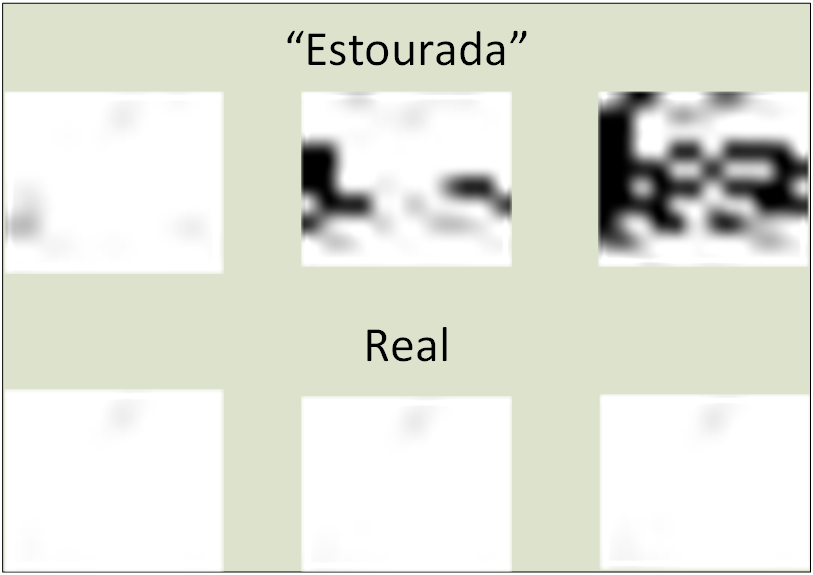
\includegraphics[scale=1]{Figuras/Image-PrevisaoEstourada.png}
	\caption{Imagem da previsão estourada}
	\label{fig:ForecastingSpike}
\end{figure}

Uma solução para este problema seria alterar o algoritmo de convolução para efetuar um processo de convolução aperiódica, que é uma forma diferente do padrão(convolução truncada, que centra a máscara com o primeiro pixel da imagem, e atribui zero aos valores inexistentes da imagem), que sempre agirá dentro da imagem porém atribui zero para resultados não calculáveis. A figura \ref{fig:convApvsTr} abaixo ilustra no seu item \emph{(a)} a convolução aperiódica, e em \emph{(b)} a convolução padrão (Truncada).

\begin{figure}[h]
	\centering	
    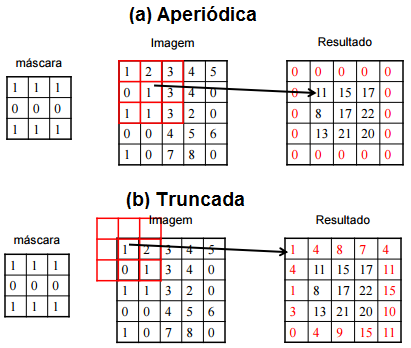
\includegraphics[scale=1]{Figuras/ConvolucaoAperiodica.png}
	\caption{Convolução aperiódica versus truncada}
	\label{fig:convApvsTr}
\end{figure}

A opção de utilizar esta forma de convolução não se aplicaria para a previsão, pois estaria-se perdendo informação e aumentando o erro da previsão de uma forma drástica, sendo que os valores das bordas de cada região seriam 0.


\subsection{Testes sobre todas regiões}
\label{Exp:Testes sobre todas regiões}


Para cada partição, será gerado um país através do processamento no ICA, que por sua vez será usado para fazer a previsão dos \emph{nTeste} períodos desta partição. Foram  executadas duas configurações de treino, sendo a primeira com apenas a condição de paradas por máxima quantidade de décadas, com os valores do ICA configurados como:

\begin{itemize}
\item Vetor de atributos do país:

  \begin{itemize}
  \item Os valores de fator estão limitados em [-50,50];
  \item Os valores das matrizes de convolução são estão limitados em [-100,100];
  \end{itemize}

\item valores das propriedades do ICA:

  \begin{itemize}
  \item Beta: 2;
  \item Taxa de revolução: 0.99;
  \item Taxa de decaimento de revolução: 0.999999;
  \item Taxa de impérios iniciais: 15\%.
  \item É Paralelo? sim;
  \item População inicial: 64;
  \item Máximo de décadas: 2048;
  \item Modo de movimento: Combinado(Refinado + Visão Imperial Distorcida);
  \end{itemize}

\end{itemize}

Para a segunda configuração, foi implementada uma condição de parada que leva em consideração o número máximo de décadas e o custo mínimo a ser atingido. Esta condição de parada segue o padrão de validação segundo o algoritmo \ref{alg:FpCP} apresentado abaixo:
	
 \begin{algorithm}[h]
\SetAlgoLined
\KwData
{
\\ \emph{curD} - década atual.
\\ \emph{maxD} - número máximo de décadas.
\\ \emph{curC} - custo do melhor país.
\\ \emph{minC} - valor do custo mínimo.
}
\KwResult{ 
\\ retorna se a condição de parada foi atingida ou não. 
}
	\Se{$curD$ >= $maxD$ * 10} 
    {
    	\KwRetorna Condição de parada atingida\;
    }
    \Se{$curD$ > $maxD$}
    {
    	\Se{$curC$ < $minC$}
     	{
        	\KwRetorna Condição de parada atingida\;
        }
    }
   \KwRetorna Condição de parada NÃO atingida\;

 \caption{Algoritmo condição de parada para o ICA}
\label{alg:FpCP}
\end{algorithm}

Observa-se no algoritmo da condição de parada que ela só será atingida quando atingir 10 vezes o número de máximo de décadas estipulado ou quando o custo for menor que \emph{minC} e, inclusivamente, o número de décadas for maior que o número máximo de décadas estipulado. Assim, garante-se que o algoritmo só irá parar segundo estas condições, tal que considera-se importante atingir o valor \emph{maxD} de décadas mesmo se o custo for menor que o valor definido em  \emph{minC}, e ainda tenta-se atingir \emph{minC} até 10 vezes o valor estipulado em \emph{maxD}. É importante mencionar que se um país chegar ao custo zero, o ICA para imediatamente, por este ser o melhor país (melhor solução a ser encontrada), e ainda, esta condição não é avaliada junto das condições de parada, mas sim antes de começar tal avaliação.

Esta segunda configuração não difere muito da primeira em questão dos parâmetros do ICA, basicamente insere-se esta nova condição de parada, que fica como:

\begin{itemize}
\item Vetor de atributos do país:

	\begin{itemize}
	\item mesmos valores;
	\end{itemize}

\item valores das propriedades do ICA:

	\begin{itemize}
	\item mesmos valores;
	\item Adicionar condição de parada 	padrão por número máximo de décadas: Não; 
	\item Usar condição de parada por década e Custo: Sim;
	\item Condição de parada adicional (por década e custo):

		\begin{itemize}
		\item Custo mínimo = 50;
		\item Máximo de décadas = 2048;
		\end{itemize}

	\end{itemize}

\end{itemize}

Geralmente, os países não convergem para custo 0, mas geram mapas com uma diferença mínima entre os períodos, de modo que este país quando utilizado para fazer uma previsão futura, seguirá o padrão de crescimento, elevando os valores de cada quadrícula de acordo com a função de testes descrita, que neste caso é a própria função que faz a previsão da expansão urbana, que usa o país como solução ótima aplicada sobre os dados, operando a ponderação das convoluções e gerando um mapa final de previsão.

Esta segunda configuração, apesar de parecer mais rápida, acaba sendo mais demorada por permitir que o número máximo de décadas se estenda para 10 vezes o tamanho configurado inicialmente. Porém, obtém-se uma previsão mais precisa em troca de tempo de processamento.

Em posse dos melhores países para cada partição, inicia-se o processo de geração dos \emph{nTest} mapas de previsão, também para cada partição. Assim que os mapas de previsão para cada partição são gerados, pode-se compará-los com com os mapas particionados reais, tomando a diferença absoluta entre a soma das diferenças das quadrículas (ou \emph{pixels}) dos mapas como sendo o erro de previsão daquela partição. 

Ao considerar cada partição como um bloco fechado, que cresce em densidade durante os períodos, tal bloco deve seguir uma linha de crescimento tendenciosa, que define em quantidades absolutas como tal bloco se desenvolverá durante períodos futuros. Mas é impossível saber, dentro deste bloco, onde e como tal crescimento será imposto. A linha de tendência sobre o crescimento do bloco fornece apenas um valor unitário de intensidade sobre como tal bloco se desenvolverá no futuro, de modo que só se pode afirmar, que todos os pontos (\emph{pixels} ou quadrículas) deste bloco irão crescer de um valor x para um valor x+y, seguindo especificamente a função de crescimento gerada pela curva de tendência linear. 

O modelo proposto, então apresenta uma solução para que se possa obter tal nível de precisão, de modo que os blocos, tenham um crescimento que siga tal linha de tendência, mesmo que a função de avaliação não os considere, e que além disso, apresentem uma solução que leve em consideração os pontos contidos no bloco, suas posições, intensidades e características regionais, dentro deste bloco, e portanto possibilitando a construção de um mapa de quadrículas disposto bidimensionalmente em forma de uma imagem, onde cada quadrícula pode ser representada por um pixel dessa imagem. Assim a análise de previsão desta metodologia utiliza-se de dois parâmetros para comparar a previsão, sendo o crescimento geral da região durante os períodos e o valor absoluto de acerto ponto a ponto.

Dentro deste cenário foram efetuados diversos testes, variando o tamanho da matriz de convolução, e a quantidade de ponderações. Foi definido que o número de ponderações igual a 3 é suficiente para prover suavidade e precisão no mapa de previsão gerado em relação aos métodos convencionais para geração do mapa de previsão. O uso de apenas um fator e uma matriz de convolução pode resultar algumas vezes, em um mapa de previsão semelhante ao modelo estatístico, que usa a curva de tendência (neste caso qualquer que seja, linear, exponencial, polinomial etc.) referente ao crescimento da região, mas não é tão preciso quando refere-se à constituição (forma e intensidade dos pontos) do mapa, relativo a quantidade de pontos, seja ela percentual ou absoluta, acertados pela previsão. O ponto negativo é que quanto mais ponderações houver, mais aumenta-se o uso de processamento, colocando mais precisamente, a quantidade de convoluções aumenta de acordo com o número de ponderações, sendo que a operação de convolução é o processo mais pesado que ocorre durante a avaliação, que por sua vez aumenta o tempo de execução de todo o processo de avaliação.

O aumento da ordem da matriz de convolução aumenta drasticamente o tempo de processamento, porém traz resultados mais interessantes. Quando seleciona-se o tamanho mínimo de 3 para a ordem da matriz de convolução, os resultados apresentados já são satisfatórios e apresentam uma precisão no acerto sobre o crescimento geral da região e sobre a quantidade de acertos ponto a ponto melhor que a curva de tendência aplicada sobre a mesma região. Ao aumentar a ordem da matriz de convolução para 5, tem-se uma melhora no erro do crescimento da região em relação à matriz de ordem 3, porém aumenta-se sutilmente o erro da previsão ponto a ponto. Aumentando a ordem da matriz para 7, algumas regiões passam a apresentar um comportamento atípico, fazendo com que o resultado final de previsão exploda para valores de erros, tanto no crescimento regional geral quanto no ponto a ponto, muito maiores que os apresentados pelo modelo estatístico, tornando o mapa final de previsão muito ruidoso e impossível de ser usado para fazer qualquer tipo de análise. A figura \ref{fig:allResults} mostra uma comparação entre os valores reais, os resultados gerados pela metodologia de previsão proposta, usando matrizes de convolução 3x3, 5x5, 7x7, com o modelo estatístico, para os anos de 2013, 2014 e 2015.

\begin{figure}[h]
	\centering	
    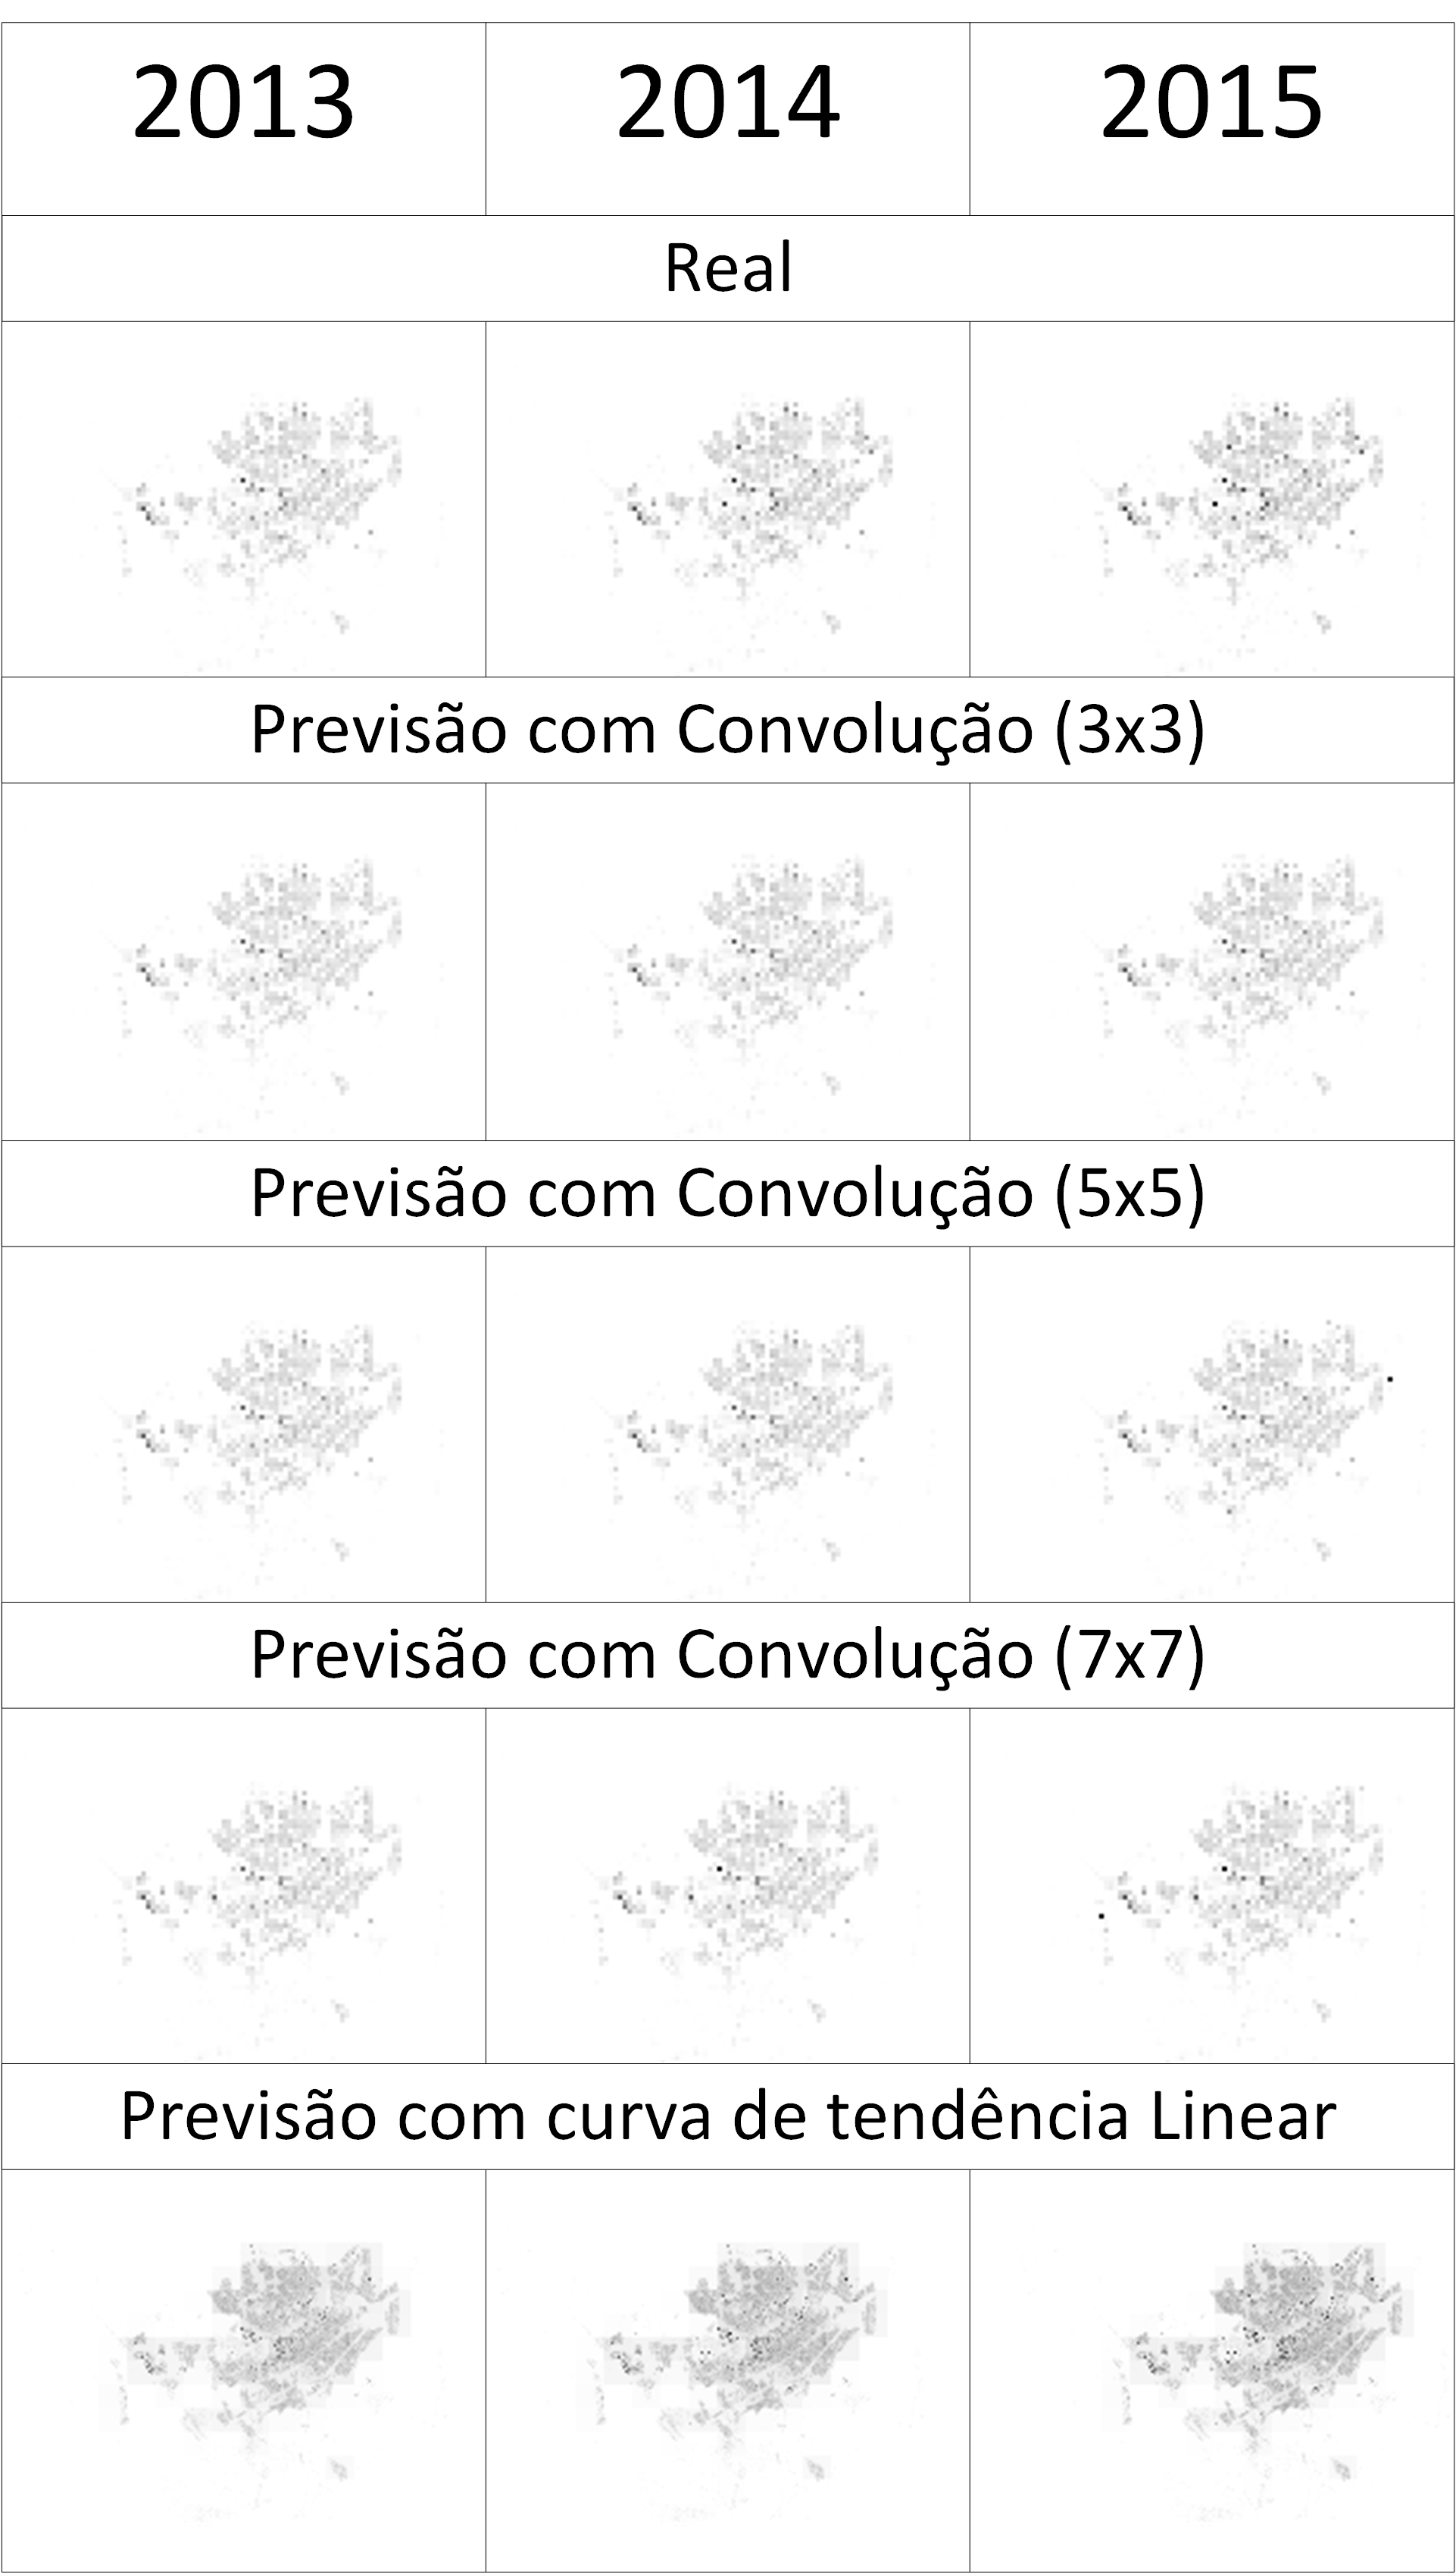
\includegraphics[scale=0.7]{Figuras/AllResults.png}
	\caption{Apresentação dos mapas reais de 2013, 2014 e 2015 comparando com a previsão por linha de tendência e com o método proposto para matrizes de convolução de ordem 3, 5 e 7}
	\label{fig:allResults}
\end{figure}

Dois parâmetros foram numericamente comparados: o erro sobre a taxa de crescimento da região prevista (Eg), e a precisão da previsão de cada célula da região (Epp). A tabela \ref{tbl:forecastErrors} mostra faz uma comparação entre os 4 métodos (proposto 3x3, proposto 5x5, proposto 7x7 e curva de tendência), onde é possível observar que o método proposto apresenta uma precisão muito semelhante em relação à linha de tendência quando compara-se o crescimento geral da região, e apresenta ainda, na previsão ponto a ponto (sobre cada célula ou \emph{pixel}) valores notavelmente melhores. Na comparação deste segundo parâmetro é possível observar ainda que ao aumentar-se a ordem da matriz de convolução não necessariamente piora-se a previsão, porém é importante notar que este aumento pode vir a extrapolar a previsão e fazer com que a precisão seja invalidada, apresentando uma previsão "estourada" como fora visto na \ref{fig:ForecastingSpike}. Os valores da matriz 5x5 apresentam-se um pouco piores, devido exatamente à extrapolação na previsão do período de 2015, sendo que na figura \ref{fig:allResults} é possível observar alguns pontos de crescimento nunca vieram a ocorrer em determinadas regiões no mapa real ou nos mapas previstos usando as matrizes de convolução de ordem 3 e 7. 

\begin{table}[h]
	\centering
	\caption{Erros de previsão}
	\label{tbl:forecastErrors}
	\begin{tabular}{l|l|l|l|l|l|}
		\cline{2-6}
		& Ano  & Eg & Eg\% & Epp & Epp\% \\ \hline
		\multicolumn{1}{|c|}{\multirow{3}{*}{Matriz 3x3}}         & 2013 & 3407,36  & 8,38\%  & 7044,81  & 2,46\%  \\ \cline{2-6} 
		\multicolumn{1}{|c|}{}                                    & 2014 & 9240,26  & 18,52\% & 14717,04 & 5,14\%  \\ \cline{2-6} 
		\multicolumn{1}{|c|}{}                                    & 2015 & 15614,48 & 26,13\% & 23649,79 & 8,27\%  \\ \hline
		\multicolumn{1}{|c|}{\multirow{3}{*}{Matriz 5x5}}         & 2013 & 3640,63  & 8,84\%  & 7359,92  & 2,57\%  \\ \cline{2-6} 
		\multicolumn{1}{|c|}{}                                    & 2014 & 9574,66  & 19,25\% & 15303,43 & 5,35\%  \\ \cline{2-6} 
		\multicolumn{1}{|c|}{}                                    & 2015 & 21038,39 & 28,86\% & 29585,02 & 10,34\% \\ \hline
		\multicolumn{1}{|c|}{\multirow{3}{*}{Matriz 7x7}}         & 2013 & 3326,51  & 8,80\%  & 7306,07  & 2,55\%  \\ \cline{2-6} 
		\multicolumn{1}{|c|}{}                                    & 2014 & 9355,60  & 18,52\% & 15325,48 & 5,36\%  \\ \cline{2-6} 
		\multicolumn{1}{|c|}{}                                    & 2015 & 16181,37 & 26,27\% & 24992,63 & 8,73\%  \\ \hline
		\multicolumn{1}{|c|}{\multirow{3}{*}{Linha de Tendência}} & 2013 & 3699,5   & 8,93\%  & 89488,3  & 31,28\% \\ \cline{2-6} 
		\multicolumn{1}{|c|}{}                                    & 2014 & 9300,8   & 18,52\% & 95026,6  & 33,21\% \\ \cline{2-6} 
		\multicolumn{1}{|c|}{}                                    & 2015 & 15757,1  & 23,15\% & 100564,9 & 35,15\% \\ \hline
	\end{tabular}
	\\[10pt]
	Nota: Validação dos resultados apresentando os erros de crescimento (Eg e Eg\%) e por pixel (Epp e Epp\%) entre o método proposto com as matrizes de convolução de ordem 3, 5 e 7 e Linha de Tendência para as previsões de 2013, 2014 e 2015
\end{table}



% ----------------------------------------------------------------
% Das conclusões tiradas
% ----------------------------------------------------------------
\chapter{Conclusão}
\label{conclusao}

Este trabalho apresenta uma abordagem evolucionária por matrizes de convolução para previsão espacial de densidades quaisquer, enfatizando em seus exemplos a densidade de carga elétrica regional. Esta abordagem usa dados históricos de pontos de instalação elétrica de diversos tipos (residencial, comercial, industrial, etc.), sendo tais dados podendo ser inseridos de qualquer fonte em uma forma normalizada pelas coordenadas geográficas, valor de densidade, tipo e  data. Quando comparado com dados históricos reais de uma cidade de tamanho médio, obtiveram resultados de alta qualidade com um erro espacial total menor que 9 \%, mesmo com acúmulo de cálculos para 3 anos consecutivos. 

A metodologia proposta utilizou quadriculas com área de 100 \(m^2\) para mapas em alta resolução, subdividos em agrupamentos planares, deta forma, obtendo um melhor impacto na previsão por adquirir características regionais mais próximas dos grupos analisados. De tal forma que o processamento e a obtenção das parâmetros de crescimento fossem obtidas através de uma otimização regional, resultando assim em diversas sub-regiões, que nos testes eram compostas de aproximadamente 130 quadriculas, podendo variar devido às bordas não serem proporcionais ao valor escolhido para a divisão das sub-regiões. Onde cada agrupamento regional tem seus próprios padrões na previsão de crescimento.

A partir deste tratamento dos mapas históricos observou-se uma função de previsão capaz de executar uma estimativa futura para um período anual \(t_{(x+1)}\), tal que esta função tenha como parâmetros um mapa de quadrículas para o ano \(t_{(x)}\) e um conjunto de informações otimizados pelo ICA, usados para formar os índices e matrizes de convolução.  

A função de previsão ainda foi adaptada para sua utilização na otimização do ICA como sendo a função de avaliação principal do problema. Assim, os parâmetros dinâmicos gerados pelas matrizes de convolução, fossem alterados e pontuados por uma \emph{regressão espacial}, onde tais parâmetros fossem modificados pela passagem desta função de avaliação por todo histórico de mapas anteriores à previsão. 

A proposta ainda demonstrou duas otimizações no ICA sobre a otimização dos valores da função de avaliação, que solucionou o problema de dimensionalidade da solução candidata pelo acrescimo de um ruído gaussiano durante a exploração do espaço de busca. A combinação dos dois métodos apresentam uma melhora ainda mais significativa na convergência para a melhor solução, como foram mostrados nos testes. 

O método proposto obteve vantagens significativas no quesito de crescimento quadrícula a quadrícula quando comparado com a previsão por curva de tendência, uma vez que as quadrículas não seguem uma função de crescimento uniforme em suas vizinhanças gerando distorções em seus índices e reduzindo a resolução do mapa futuro. Fato que não ocorre dentro da metodologia proposta com matrizes de convolução.

A maior dificuldade encontrada no trabalho foi a aquisição das informações georeferenciadas necessárias para o início dos estudos, pois mesmo com os diversos mapas disponíveis on-line, os dados de densidade populacional e a proporcional densidade de carga elétrica requer um estudo das imagens da região. Logo foi executado uma extração manual desses dados dos mapas de satélite para obter os campos de latitude, longitude, tipo de consumidor, data do mapa e densidade necessários para os testes.

O esforço computacional da metodologia com matrizes de convolução é extremamente alto, devido à busca de correlação dos mapas históricos em quadrículas para a extração dos melhores padrões em matrizes. Assim essa operação leva aproximadamente de 2 a 3 horas de processamento paralelo para todas as 225 regiões do teste, em um computador com Windows 10 e processador AMD-FX8350 de 8 núcleos com clock fixo de 3GHz e 16GB RAM, calculando a matriz de convolução de ordem 7 com 3 ponderações. Como o código do ICA foi desenvolvido de forma a ser otimizado em relação às suas operações internas, 93\% do tempo total é ocasionado pelo cálculo paralelo da função de avaliação, que realiza inúmeras operações matriciais com os mapas históricos de quadrículas. Como exemplo, o número de operações de convolução que ocorrem durante uma década é igual ao número de colônias vezes o número de ponderações escolhidas. É importante salientar que mesmo com um alto tempo de cálculo a metodologia proposta é paralela, permitindo sua utilização em núvens de clusters de computadores, reduzindo de forma abrupta esse tempo de cálculo obtido nos experimentos.

O destaque da proposta fica evidente pela qualidade dos resultados gerados, tanto pela alta resolução quanto pelo alto grau de acerto, obtidos pelas contribuições no uso de matrizes de convolução para identificação e cálculo dos padrões de crescimento das áreas, quanto a eficiência e robustez do ICA para a busca dessas matrizes em um problema tão grande e complexo em proporções.

A aplicação desses resultados são de grande valia para as empresas concessionárias de energia, pois com a qualidade de valores futuros e a grande resolução de seus mapas permitem o planejamento da expansão do sistema elétrico de um município, identificando com precisão locais de novas subestações, instalação de novos transformadores e a inserção de acumuladores com baterias de sal em locais estratégicos, aumentando a confiabilidade da rede e reduzindo custos.

Inicialmente proposta para o emprego em Smartgrids, o previsor espacial urbano durante os estudos demonstrou um emprego muito mais amplo além do foco em mercados consumidores de energia por sua resolução mais apurada nos mapas futuros. Planejamentos urbanos de vias, serviços fundamentais como escolas e clínicas, fornecimento de comunicação, água e gás podem utilizar sem nenhuma modificação a metodologia proposta, demonstrando ser uma ferramenta poderosa para a solução dos principais problemas urbanos encontrados em nossas cidades. 

\section{Colaborações do Trabalho}
\label{colaborações_do_trabalho}

% ICA modificado + matriz de convolução para identificação de características do mapa %

Este trabalho apresenta duas colaborações relevantes, sendo a primeira a resolução do problema da dimensionalidade dos limites dos atributos do ICA, que fora solucionado com duas implementações distintas, podendo elas serem utilizadas separadamente ou de forma combinada, alterando diretamente a forma como os ruídos são inseridos durante a assimilação de colônias por um império, diminuindo o tempo de conversão, em número de décadas, para o mínimo global. Além disso, o ICA foi desenvolvido de forma a ser facilmente utilizado por qualquer aplicação, isolando a sua lógica do processo evolutivo do problema a ser implementado, de modo que, qualquer problema que venha a ser modelado no ICA não precise alterar os componentes relativos ao processo evolutivo. 

A segunda colaboração deste trabalho é referente à forma como foram usadas as operações de convolução, sendo estas combinadas em uma função de previsão, que faz ponderações sobre diversas matrizes de convolução, que neste caso são treinadas pelo ICA com o intuito de obter características de crescimento de densidade distintas de uma mesma região, as quais, junto de outros atributos, são usadas para formar um mapa futuro de previsão. Com a operação de convolução, é possível buscar tais características de crescimento para cada ponto de modo que tanto o ponto em questão quanto os pontos vizinhos sejam levados em consideração no momento da definição da característica, durante a etapa de treino. A ponderação entre as diversas matrizes de convolução garante que a previsão de um dado ponto condiz mais com a realidade, dentre diversas características.

\section{Trabalhos Futuros}
\label{trabalhos_futuros}

Este trabalho aplicou a função de previsão sobre os dados de densidade de carga elétrica. Porém, tal técnica pode ser utilizada para a busca de um mapa de crescimento futuro baseado em qualquer tipo de densidade. Para trabalhos futuros tem-se a intenção de alterar a função de previsão para que esta faça o uso de outra técnica de processamento de imagens ou até mesmo, que venha a utilizar técnicas de visão computacional, como a identificação de padrões através de técnicas do tipo Haar \cite{mita2005joint}, que geralmente são utilizadas para encontrar padrões faciais, porém podem ser aplicadas para o treinamento e reconhecimento de qualquer tipo de padrão em imagens, sendo possível a detecção de padrões de crescimento sobre a identificação de padrões na forma e intensidade dos pontos da imagem, diminuindo a quantidade de parâmetros, porém aumentando a quantidade de características de crescimento de uma região.


% haar-feature para identificação de padrões para regiões de crescimento %


\bibliography{bibliografia}

%% ----------------------------------------------------------------
% Os documentos e imagens adicionais da dissertação
% ----------------------------------------------------------------
\apendice

\chapter{Tabelas dos Valores Obtidos nos Testes}
\label{apendice_tabelas_valores}

As tabelas a seguir apresentam o Valor Obtido ($v_i$), o Valor Médio Acumulado ($VMA_i$) e a Variação de Valor Médio Acumulado ($Var_i$) em todas as métricas, para cada uma das execuções realizadas. As iterações encerram quando todas as métricas obtém Variação de Valor Médio Acumulado ($Var_i$) com valor igual ou inferior a 5\% (0.05) em duas iterações seguidas. O número mínimo de 5 execuções foi utilizado.

A Tabela abaixo é um modelo de representação das tabelas a seguir.

\begin{table}[htb]
\rowcolors{2}{gray!25}{white}
\centering
\resizebox{\textwidth}{!}{%
\begin{tabular}{ccllllll}
\rowcolor{gray!50}
\hline
\multicolumn{1}{c|}{Execução} & \multicolumn{1}{c|}{\begin{tabular}[c]{@{}c@{}}Nota de\\ Avaliação\\ Média\end{tabular}} & \multicolumn{1}{c|}{\begin{tabular}[c]{@{}c@{}}Dispersão\\ Média\end{tabular}} & \multicolumn{1}{c|}{\begin{tabular}[c]{@{}c@{}}Nota Local\\ Média\end{tabular}} & \multicolumn{1}{c|}{\begin{tabular}[c]{@{}c@{}}Nota Local\\ Máxima\end{tabular}} & \multicolumn{1}{c|}{$C_f$ Count} & \multicolumn{1}{c|}{\begin{tabular}[c]{@{}c@{}}Nota de\\ Avaliação\\ em $C_f$\end{tabular}} & \multicolumn{1}{c}{\begin{tabular}[c]{@{}c@{}}Dispersão\\ em $C_f$\end{tabular}} \\ \hline
\multicolumn{1}{c|}{} & \multicolumn{7}{c|}{Valores Obtido nesta Execução ($v$)} \\ \cline{2-8} 
\multicolumn{1}{c|}{} & \multicolumn{7}{c|}{Valores Médios Acumulados ($VMA$)} \\ \cline{2-8} 
\multicolumn{1}{c|}{\multirow{-3}{*}{1}} & \multicolumn{7}{c|}{Variação de Valor Médio Acumulado em relação à execução anterior ($Var$)} \\ \hline
\multicolumn{1}{c|}{...} & \multicolumn{1}{l|}{} & \multicolumn{1}{l|}{} & \multicolumn{1}{l|}{} & \multicolumn{1}{l|}{} & \multicolumn{1}{l|}{} & \multicolumn{1}{l|}{} &  \\ \hline
\multicolumn{1}{c|}{} & \multicolumn{7}{c|}{$v_i$} \\ \cline{2-8} 
\multicolumn{1}{c|}{} & \multicolumn{7}{c|}{${VMA}_i = (v_1 + v_2 + ... + v_{i-1} + v_i) / i$} \\ \cline{2-8} 
\multicolumn{1}{c|}{\multirow{-3}{*}{i}} & \multicolumn{7}{c|}{${Var}_i = ({VMA}_i / {VMA}_{i-1}) - 1$} \\ \hline
\multicolumn{1}{c|}{...} & \multicolumn{1}{r|}{} & \multicolumn{1}{r|}{} & \multicolumn{1}{r|}{} & \multicolumn{1}{r|}{} & \multicolumn{1}{r|}{} & \multicolumn{1}{r|}{} & \multicolumn{1}{r}{} \\ \hline
\multicolumn{1}{c|}{} & \multicolumn{7}{c|}{$v_{n-1}$} \\ \cline{2-8} 
\multicolumn{1}{c|}{} & \multicolumn{7}{c|}{${VMA}_{n-1}$} \\ \cline{2-8} 
\multicolumn{1}{c|}{\multirow{-3}{*}{n-1}} & \multicolumn{7}{c|}{\cellcolor[HTML]{ADDDAD}$|{Var}_{n-1}| \leq 0.05$} \\ \hline
\multicolumn{1}{c|}{} & \multicolumn{7}{c|}{$v_n$} \\ \cline{2-8} 
\multicolumn{1}{c|}{} & \multicolumn{7}{c|}{\cellcolor[HTML]{FFCE93}${VMA}_n$} \\ \cline{2-8} 
\multicolumn{1}{c|}{\multirow{-3}{*}{n}} & \multicolumn{7}{c|}{\cellcolor[HTML]{ADDDAD}$|{Var}_n| \leq 0.05$} \\ \hline 
\multicolumn{1}{l}{} & \multicolumn{1}{l}{} &  &  &  &  &  &  \\ \cline{2-4} \cline{6-8} 
\multicolumn{1}{l|}{\cellcolor[HTML]{FFFFFF}} & \multicolumn{3}{c|}{\cellcolor[HTML]{ADDDAD}Variação abaixo de 5\%} & \multicolumn{1}{l|}{\cellcolor[HTML]{FFFFFF}} & \multicolumn{3}{c|}{\cellcolor[HTML]{FFCE93}Valores utilizados} \\ \cline{2-4} \cline{6-8} 
\end{tabular}%
}
\end{table}

\pagebreak

\section{Algoritmo Genético}

Os valores de Nota de Avaliação em $C_f$ e Dispersão em $C_f$ não se aplicam à configuração \textbf{AG} conforme discutido na seção \ref{metricas}.

\begin{table}[!htb]
\rowcolors{2}{gray!25}{white}
\centering
\resizebox{\textwidth}{!}{%
\begin{tabular}{c|r|r|r|r|r|r|r}
\rowcolor{gray!50}
\hline
Execução & \multicolumn{1}{c|}{\begin{tabular}[c]{@{}c@{}}Nota de\\ Avaliação\\ Média\end{tabular}} & \multicolumn{1}{c|}{\begin{tabular}[c]{@{}c@{}}Dispersão\\ Média\end{tabular}} & \multicolumn{1}{c|}{\begin{tabular}[c]{@{}c@{}}Nota Local\\ Média\end{tabular}} & \multicolumn{1}{c|}{\begin{tabular}[c]{@{}c@{}}Nota Local\\ Máxima\end{tabular}} & \multicolumn{1}{c|}{$C_f$ Count} & \multicolumn{1}{c|}{\begin{tabular}[c]{@{}c@{}}Nota de\\ Avaliação\\ em $C_f$\end{tabular}} & \multicolumn{1}{c}{\begin{tabular}[c]{@{}c@{}}Dispersão\\ em $C_f$\end{tabular}} \\ \hline
 & 255.3900 & 43.0220 & 2.1450 & 15.0000 & 1.0000 & - & - \\ \cline{2-8} 
 & 255.3900 & 43.0220 & 2.1450 & 15.0000 & 1.0000 & - & - \\ \cline{2-8} 
\multirow{-3}{*}{1} & - & - & - & - & - & - & - \\ \hline
 & 292.3300 & 21.9953 & 0.5250 & 6.0000 & 0.0000 & - & - \\ \cline{2-8} 
 & 258.8600 & 32.5087 & 1.3350 & 10.5000 & 0.5000 & - & - \\ \cline{2-8} 
\multirow{-3}{*}{2} & 0.1485 & -0.2444 & -0.3776 & -0.3000 & -0.5000 & - & - \\ \hline
 & 263.7850 & 17.9270 & 0.8650 & 10.0000 & 0.0000 & - & - \\ \cline{2-8} 
 & 260.5017 & 27.6481 & 1.1783 & 10.3333 & 0.3333 & - & - \\ \cline{2-8} 
\multirow{-3}{*}{3} & \cellcolor[HTML]{ADDDAD}0.0063 & -0.1495 & -0.1174 & \cellcolor[HTML]{ADDDAD}-0.0159 & -0.3333 & - & - \\ \hline
 & 237.0050 & 28.4870 & 0.0750 & 15.0000 & 1.0000 & - & - \\ \cline{2-8} 
 & 254.6275 & 27.8578 & 0.9025 & 11.5000 & 0.5000 & - & - \\ \cline{2-8} 
\multirow{-3}{*}{4} & \cellcolor[HTML]{ADDDAD}-0.0225 & \cellcolor[HTML]{ADDDAD}0.0076 & -0.2341 & 0.1129 & 0.5000 & - & - \\ \hline
 & 260.0000 & 10.6010 & 0.0000 & 0.0000 & 0.0000 & - & - \\ \cline{2-8} 
 & 255.7020 & 24.4065 & 0.7220 & 9.2000 & 0.4000 & - & - \\ \cline{2-8} 
\multirow{-3}{*}{5} & \cellcolor[HTML]{ADDDAD}0.0042 & -0.1239 & -0.2000 & -0.2000 & -0.2000 & - & - \\ \hline
 & 241.0000 & 118.8943 & 0.0000 & 0.0000 & 0.0000 & - & - \\ \cline{2-8} 
 & 253.2517 & 40.1544 & 0.6017 & 7.6667 & 0.3333 & - & - \\ \cline{2-8} 
\multirow{-3}{*}{6} & \cellcolor[HTML]{ADDDAD}-0.0096 & 0.6452 & -0.1667 & -0.1667 & -0.1667 & - & - \\ \hline
 & 208.2350 & 40.6240 & 0.1500 & 15.0000 & 2.0000 & - & - \\ \cline{2-8} 
 & 246.8207 & 40.2215 & 0.5371 & 8.7143 & 0.5714 & - & - \\ \cline{2-8} 
\multirow{-3}{*}{7} & \cellcolor[HTML]{ADDDAD}-0.0254 & \cellcolor[HTML]{ADDDAD}0.0017 & -0.1072 & 0.1366 & 0.7143 & - & - \\ \hline
 & 226.1050 & 31.7023 & 0.2800 & 15.0000 & 1.0000 & - & - \\ \cline{2-8} 
 & 244.2313 & 39.1566 & 0.5050 & 9.5000 & 0.6250 & - & - \\ \cline{2-8} 
\multirow{-3}{*}{8} & \cellcolor[HTML]{ADDDAD}-0.0105 & \cellcolor[HTML]{ADDDAD}-0.0265 & -0.0598 & 0.0902 & 0.0938 & - & - \\ \hline
 & 277.3150 & 38.7190 & 0.7550 & 14.0000 & 0.0000 & - & - \\ \cline{2-8} 
 & 247.9072 & 39.1080 & 0.5328 & 10.0000 & 0.5556 & - & - \\ \cline{2-8} 
\multirow{-3}{*}{9} & \cellcolor[HTML]{ADDDAD}0.0151 & \cellcolor[HTML]{ADDDAD}-0.0012 & 0.0550 & 0.0526 & -0.1111 & - & - \\ \hline
 & 228.0000 & 29.9807 & 0.0000 & 0.0000 & 0.0000 & - & - \\ \cline{2-8} 
 & 245.9165 & 38.1953 & 0.4795 & 9.0000 & 0.5000 & - & - \\ \cline{2-8} 
\multirow{-3}{*}{10} & \cellcolor[HTML]{ADDDAD}-0.0080 & \cellcolor[HTML]{ADDDAD}-0.0233 & -0.1000 & -0.1000 & -0.1000 & - & - \\ \hline
 & 240.0050 & 29.3243 & 0.0750 & 15.0000 & 1.0000 & - & - \\ \cline{2-8} 
 & 245.3791 & 37.3888 & 0.4427 & 9.5455 & 0.5455 & - & - \\ \cline{2-8} 
\multirow{-3}{*}{11} & \cellcolor[HTML]{ADDDAD}-0.0022 & \cellcolor[HTML]{ADDDAD}-0.0211 & -0.0767 & 0.0606 & 0.0909 & - & - \\ \hline
 & 271.7650 & 62.5497 & 1.6800 & 15.0000 & 3.0000 & - & - \\ \cline{2-8} 
 & 247.5779 & 39.4865 & 0.5458 & 10.0000 & 0.7500 & - & - \\ \cline{2-8} 
\multirow{-3}{*}{12} & \cellcolor[HTML]{ADDDAD}0.0090 & 0.0561 & 0.2329 & \cellcolor[HTML]{ADDDAD}0.0476 & 0.3750 & - & - \\ \hline
 & 235.0000 & 17.3193 & 0.0000 & 0.0000 & 0.0000 & - & - \\ \cline{2-8} 
 & 246.6104 & 37.7805 & 0.5038 & 9.2308 & 0.6923 & - & - \\ \cline{2-8} 
\multirow{-3}{*}{13} & \cellcolor[HTML]{ADDDAD}-0.0039 & \cellcolor[HTML]{ADDDAD}-0.0432 & -0.0769 & -0.0769 & -0.0769 & - & - \\ \hline
 & 233.0050 & 10.1877 & 0.0750 & 15.0000 & 1.0000 & - & - \\ \cline{2-8} 
 & 245.6386 & 35.8095 & 0.4732 & 9.6429 & 0.7143 & - & - \\ \cline{2-8} 
\multirow{-3}{*}{14} & \cellcolor[HTML]{ADDDAD}-0.0039 & -0.0522 & -0.0608 & \cellcolor[HTML]{ADDDAD}0.0446 & \cellcolor[HTML]{ADDDAD}0.0317 & - & - \\ \hline
\end{tabular}%
}
\end{table}

\FloatBarrier
\pagebreak

\begin{table}[htb]
\rowcolors{2}{gray!25}{white}
\centering
\resizebox{\textwidth}{!}{%
\begin{tabular}{c|r|r|r|r|r|r|r}
\rowcolor{gray!50}
\hline
Execução & \multicolumn{1}{c|}{\begin{tabular}[c]{@{}c@{}}Nota de\\ Avaliação\\ Média\end{tabular}} & \multicolumn{1}{c|}{\begin{tabular}[c]{@{}c@{}}Dispersão\\ Média\end{tabular}} & \multicolumn{1}{c|}{\begin{tabular}[c]{@{}c@{}}Nota Local\\ Média\end{tabular}} & \multicolumn{1}{c|}{\begin{tabular}[c]{@{}c@{}}Nota Local\\ Máxima\end{tabular}} & \multicolumn{1}{c|}{$C_f$ Count} & \multicolumn{1}{c|}{\begin{tabular}[c]{@{}c@{}}Nota de\\ Avaliação\\ em $C_f$\end{tabular}} & \multicolumn{1}{c}{\begin{tabular}[c]{@{}c@{}}Dispersão\\ em $C_f$\end{tabular}} \\ \hline
 & 217.0000 & 48.4733 & 0.0000 & 0.0000 & 0.0000 & - & - \\ \cline{2-8} 
 & 243.7293 & 36.6538 & 0.4417 & 9.0000 & 0.6667 & - & - \\ \cline{2-8} 
\multirow{-3}{*}{15} & \cellcolor[HTML]{ADDDAD}-0.0078 & \cellcolor[HTML]{ADDDAD}0.0236 & -0.0667 & -0.0667 & -0.0667 & - & - \\ \hline
 & 232.0750 & 49.5183 & 0.3600 & 13.0000 & 0.0000 & - & - \\ \cline{2-8} 
 & 243.0009 & 37.4578 & 0.4366 & 9.2500 & 0.6250 & - & - \\ \cline{2-8} 
\multirow{-3}{*}{16} & \cellcolor[HTML]{ADDDAD}-0.0030 & \cellcolor[HTML]{ADDDAD}0.0219 & \cellcolor[HTML]{ADDDAD}-0.0116 & \cellcolor[HTML]{ADDDAD}0.0278 & -0.0625 & - & - \\ \hline
 & 256.0000 & 43.4033 & 0.0000 & 0.0000 & 0.0000 & - & - \\ \cline{2-8} 
 & 243.7656 & 37.8076 & 0.4109 & 8.7059 & 0.5882 & - & - \\ \cline{2-8} 
\multirow{-3}{*}{17} & \cellcolor[HTML]{ADDDAD}0.0031 & \cellcolor[HTML]{ADDDAD}0.0093 & -0.0588 & -0.0588 & -0.0588 & - & - \\ \hline
 & 227.0000 & 44.6817 & 0.0000 & 0.0000 & 0.0000 & - & - \\ \cline{2-8} 
 & 242.8342 & 38.1895 & 0.3881 & 8.2222 & 0.5556 & - & - \\ \cline{2-8} 
\multirow{-3}{*}{18} & \cellcolor[HTML]{ADDDAD}-0.0038 & \cellcolor[HTML]{ADDDAD}0.0101 & -0.0556 & -0.0556 & -0.0556 & - & - \\ \hline
 & 243.0300 & 10.6437 & 0.1950 & 13.0000 & 0.0000 & - & - \\ \cline{2-8} 
 & 242.8445 & 36.7397 & 0.3779 & 8.4737 & 0.5263 & - & - \\ \cline{2-8} 
\multirow{-3}{*}{19} & \cellcolor[HTML]{ADDDAD}0.0000 & \cellcolor[HTML]{ADDDAD}-0.0380 & \cellcolor[HTML]{ADDDAD}-0.0262 & \cellcolor[HTML]{ADDDAD}0.0306 & -0.0526 & - & - \\ \hline
 & 250.3850 & 37.5533 & 0.6100 & 14.0000 & 0.0000 & - & - \\ \cline{2-8} 
 & 243.2215 & 36.7804 & 0.3895 & 8.7500 & 0.5000 & - & - \\ \cline{2-8} 
\multirow{-3}{*}{20} & \cellcolor[HTML]{ADDDAD}0.0016 & \cellcolor[HTML]{ADDDAD}0.0011 & \cellcolor[HTML]{ADDDAD}0.0307 & \cellcolor[HTML]{ADDDAD}0.0326 & \cellcolor[HTML]{ADDDAD}-0.0500 & - & - \\ \hline
 & 247.0100 & 17.9377 & 0.1400 & 14.0000 & 0.0000 & - & - \\ \cline{2-8} 
 & \cellcolor[HTML]{FFCE93}243.4019 & \cellcolor[HTML]{FFCE93}35.8831 & \cellcolor[HTML]{FFCE93}0.3776 & \cellcolor[HTML]{FFCE93}9.0000 & \cellcolor[HTML]{FFCE93}0.4762 & - & - \\ \cline{2-8} 
\multirow{-3}{*}{21} & \cellcolor[HTML]{ADDDAD}0.0007 & \cellcolor[HTML]{ADDDAD}-0.0244 & \cellcolor[HTML]{ADDDAD}-0.0305 & \cellcolor[HTML]{ADDDAD}0.0286 & \cellcolor[HTML]{ADDDAD}-0.0476 & - & - \\ \hline
\end{tabular}%
}
\end{table}

Tempo total de execução: 875 segundos

\pagebreak
\section{Busca Inovativa}

\begin{table}[htb]
\rowcolors{2}{gray!25}{white}
\centering
\resizebox{\textwidth}{!}{%
\begin{tabular}{c|r|r|r|r|r|r|r}
\rowcolor{gray!50}
\hline
Execução & \multicolumn{1}{c|}{\begin{tabular}[c]{@{}c@{}}Nota de\\ Avaliação\\ Média\end{tabular}} & \multicolumn{1}{c|}{\begin{tabular}[c]{@{}c@{}}Dispersão\\ Média\end{tabular}} & \multicolumn{1}{c|}{\begin{tabular}[c]{@{}c@{}}Nota Local\\ Média\end{tabular}} & \multicolumn{1}{c|}{\begin{tabular}[c]{@{}c@{}}Nota Local\\ Máxima\end{tabular}} & \multicolumn{1}{c|}{$C_f$ Count} & \multicolumn{1}{c|}{\begin{tabular}[c]{@{}c@{}}Nota de\\ Avaliação\\ em $C_f$\end{tabular}} & \multicolumn{1}{c}{\begin{tabular}[c]{@{}c@{}}Dispersão\\ em $C_f$\end{tabular}} \\ \hline
 & 55.7400 & 1695.3943 & 7.9950 & 15.0000 & 14.0000 & 90.6429 & 2028.8901 \\ \cline{2-8} 
 & 55.7400 & 1695.3943 & 7.9950 & 15.0000 & 14.0000 & 90.6429 & 2028.8901 \\ \cline{2-8} 
\multirow{-3}{*}{1} & - & - & - & - & - & - & - \\ \hline
 & 74.2200 & 1692.8953 & 8.1450 & 15.0000 & 14.0000 & 105.1429 & 2032.7143 \\ \cline{2-8} 
 & 64.9800 & 1694.1448 & 8.0700 & 15.0000 & 14.0000 & 97.8929 & 2030.8022 \\ \cline{2-8} 
\multirow{-3}{*}{2} & 0.1658 & \cellcolor[HTML]{ADDDAD}-0.0007 & \cellcolor[HTML]{ADDDAD}0.0094 & \cellcolor[HTML]{ADDDAD}0.0000 & \cellcolor[HTML]{ADDDAD}0.0000 & 0.0800 & \cellcolor[HTML]{ADDDAD}0.0009 \\ \hline
 & 62.9100 & 1702.1457 & 7.7950 & 15.0000 & 11.0000 & 109.1818 & 2053.8182 \\ \cline{2-8} 
 & 64.2900 & 1696.8118 & 7.9783 & 15.0000 & 13.0000 & 101.6558 & 2038.4742 \\ \cline{2-8} 
\multirow{-3}{*}{3} & \cellcolor[HTML]{ADDDAD}-0.0106 & \cellcolor[HTML]{ADDDAD}0.0016 & \cellcolor[HTML]{ADDDAD}-0.0114 & \cellcolor[HTML]{ADDDAD}0.0000 & -0.0714 & \cellcolor[HTML]{ADDDAD}0.0384 & \cellcolor[HTML]{ADDDAD}0.0038 \\ \hline
 & 55.1800 & 1679.0587 & 7.7450 & 15.0000 & 8.0000 & 106.1250 & 2051.1429 \\ \cline{2-8} 
 & 62.0125 & 1692.3735 & 7.9200 & 15.0000 & 11.7500 & 102.7731 & 2041.6414 \\ \cline{2-8} 
\multirow{-3}{*}{4} & \cellcolor[HTML]{ADDDAD}-0.0354 & \cellcolor[HTML]{ADDDAD}-0.0026 & \cellcolor[HTML]{ADDDAD}-0.0073 & \cellcolor[HTML]{ADDDAD}0.0000 & -0.0962 & \cellcolor[HTML]{ADDDAD}0.0110 & \cellcolor[HTML]{ADDDAD}0.0016 \\ \hline
 & 65.0550 & 1697.0447 & 7.5400 & 15.0000 & 10.0000 & 103.1000 & 2049.3778 \\ \cline{2-8} 
 & 62.6210 & 1693.3077 & 7.8440 & 15.0000 & 11.4000 & 102.8385 & 2043.1886 \\ \cline{2-8} 
\multirow{-3}{*}{5} & \cellcolor[HTML]{ADDDAD}0.0098 & \cellcolor[HTML]{ADDDAD}0.0006 & \cellcolor[HTML]{ADDDAD}-0.0096 & \cellcolor[HTML]{ADDDAD}0.0000 & \cellcolor[HTML]{ADDDAD}-0.0298 & \cellcolor[HTML]{ADDDAD}0.0006 & \cellcolor[HTML]{ADDDAD}0.0008 \\ \hline
 & 70.8900 & 1691.3567 & 8.4750 & 15.0000 & 15.0000 & 104.0000 & 2041.7905 \\ \cline{2-8} 
 & 63.9992 & 1692.9826 & 7.9492 & 15.0000 & 12.0000 & 103.0321 & 2042.9556 \\ \cline{2-8} 
\multirow{-3}{*}{6} & \cellcolor[HTML]{ADDDAD}0.0220 & \cellcolor[HTML]{ADDDAD}-0.0002 & \cellcolor[HTML]{ADDDAD}0.0134 & \cellcolor[HTML]{ADDDAD}0.0000 & 0.0526 & \cellcolor[HTML]{ADDDAD}0.0019 & \cellcolor[HTML]{ADDDAD}-0.0001 \\ \hline
 & 52.7400 & 1685.8547 & 7.9600 & 15.0000 & 11.0000 & 88.4545 & 2050.5636 \\ \cline{2-8} 
 & 62.3907 & 1691.9643 & 7.9507 & 15.0000 & 11.8571 & 100.9496 & 2044.0425 \\ \cline{2-8} 
\multirow{-3}{*}{7} & \cellcolor[HTML]{ADDDAD}-0.0251 & \cellcolor[HTML]{ADDDAD}-0.0006 & \cellcolor[HTML]{ADDDAD}0.0002 & \cellcolor[HTML]{ADDDAD}0.0000 & \cellcolor[HTML]{ADDDAD}-0.0119 & \cellcolor[HTML]{ADDDAD}-0.0202 & \cellcolor[HTML]{ADDDAD}0.0005 \\ \hline
 & 67.2900 & 1692.4190 & 7.6050 & 15.0000 & 15.0000 & 99.7333 & 2049.5143 \\ \cline{2-8} 
 & \cellcolor[HTML]{FFCE93}63.0031 & \cellcolor[HTML]{FFCE93}1692.0211 & \cellcolor[HTML]{FFCE93}7.9075 & \cellcolor[HTML]{FFCE93}15.0000 & \cellcolor[HTML]{FFCE93}12.2500 & \cellcolor[HTML]{FFCE93}100.7976 & \cellcolor[HTML]{FFCE93}2044.7265 \\ \cline{2-8} 
\multirow{-3}{*}{8} & \cellcolor[HTML]{ADDDAD}0.0098 & \cellcolor[HTML]{ADDDAD}0.0000 & \cellcolor[HTML]{ADDDAD}-0.0054 & \cellcolor[HTML]{ADDDAD}0.0000 & \cellcolor[HTML]{ADDDAD}0.0331 & \cellcolor[HTML]{ADDDAD}-0.0015 & \cellcolor[HTML]{ADDDAD}0.0003 \\ \hline
\end{tabular}%
}
\end{table}

Tempo total de execução: 1634 segundos

\pagebreak
\section{Competição Local}

\begin{table}[htb]
\rowcolors{2}{gray!25}{white}
\centering
\resizebox{\textwidth}{!}{%
\begin{tabular}{c|r|r|r|r|r|r|r}
\rowcolor{gray!50}
\hline
Execução & \multicolumn{1}{c|}{\begin{tabular}[c]{@{}c@{}}Nota de\\ Avaliação\\ Média\end{tabular}} & \multicolumn{1}{c|}{\begin{tabular}[c]{@{}c@{}}Dispersão\\ Média\end{tabular}} & \multicolumn{1}{c|}{\begin{tabular}[c]{@{}c@{}}Nota Local\\ Média\end{tabular}} & \multicolumn{1}{c|}{\begin{tabular}[c]{@{}c@{}}Nota Local\\ Máxima\end{tabular}} & \multicolumn{1}{c|}{$C_f$ Count} & \multicolumn{1}{c|}{\begin{tabular}[c]{@{}c@{}}Nota de\\ Avaliação\\ em $C_f$\end{tabular}} & \multicolumn{1}{c}{\begin{tabular}[c]{@{}c@{}}Dispersão\\ em $C_f$\end{tabular}} \\ \hline
 & 102.0000 & 1675.3643 & 9.9100 & 15.0000 & 25.0000 & 129.6400 & 2037.5533 \\ \cline{2-8} 
 & 102.0000 & 1675.3643 & 9.9100 & 15.0000 & 25.0000 & 129.6400 & 2037.5533 \\ \cline{2-8} 
\multirow{-3}{*}{1} & - & - & - & - & - & - & - \\ \hline
 & 100.2050 & 1679.6123 & 9.3900 & 15.0000 & 22.0000 & 139.5455 & 2028.9134 \\ \cline{2-8} 
 & 101.1025 & 1677.4883 & 9.6500 & 15.0000 & 23.5000 & 134.5927 & 2033.2334 \\ \cline{2-8} 
\multirow{-3}{*}{2} & \cellcolor[HTML]{ADDDAD}-0.0088 & \cellcolor[HTML]{ADDDAD}0.0013 & \cellcolor[HTML]{ADDDAD}-0.0262 & \cellcolor[HTML]{ADDDAD}0.0000 & -0.0600 & \cellcolor[HTML]{ADDDAD}0.0382 & \cellcolor[HTML]{ADDDAD}-0.0021 \\ \hline
 & 103.5150 & 1683.0843 & 9.7500 & 15.0000 & 16.0000 & 129.1250 & 2050.2750 \\ \cline{2-8} 
 & 101.9067 & 1679.3537 & 9.6833 & 15.0000 & 21.0000 & 132.7702 & 2038.9139 \\ \cline{2-8} 
\multirow{-3}{*}{3} & \cellcolor[HTML]{ADDDAD}0.0080 & \cellcolor[HTML]{ADDDAD}0.0011 & \cellcolor[HTML]{ADDDAD}0.0035 & \cellcolor[HTML]{ADDDAD}0.0000 & -0.1064 & \cellcolor[HTML]{ADDDAD}-0.0135 & \cellcolor[HTML]{ADDDAD}0.0028 \\ \hline
 & 101.5450 & 1684.4330 & 9.5450 & 15.0000 & 24.0000 & 137.5833 & 2027.3949 \\ \cline{2-8} 
 & 101.8163 & 1680.6235 & 9.6488 & 15.0000 & 21.7500 & 133.9734 & 2036.0342 \\ \cline{2-8} 
\multirow{-3}{*}{4} & \cellcolor[HTML]{ADDDAD}-0.0009 & \cellcolor[HTML]{ADDDAD}0.0008 & \cellcolor[HTML]{ADDDAD}-0.0036 & \cellcolor[HTML]{ADDDAD}0.0000 & \cellcolor[HTML]{ADDDAD}0.0357 & \cellcolor[HTML]{ADDDAD}0.0091 & \cellcolor[HTML]{ADDDAD}-0.0014 \\ \hline
 & 103.9450 & 1687.1173 & 9.5750 & 15.0000 & 26.0000 & 134.7308 & 2029.9354 \\ \cline{2-8} 
 & \cellcolor[HTML]{FFCE93}102.2420 & \cellcolor[HTML]{FFCE93}1681.9223 & \cellcolor[HTML]{FFCE93}9.6340 & \cellcolor[HTML]{FFCE93}15.0000 & \cellcolor[HTML]{FFCE93}22.6000 & \cellcolor[HTML]{FFCE93}134.1249 & \cellcolor[HTML]{FFCE93}2034.8144 \\ \cline{2-8} 
\multirow{-3}{*}{5} & \cellcolor[HTML]{ADDDAD}0.0042 & \cellcolor[HTML]{ADDDAD}0.0008 & \cellcolor[HTML]{ADDDAD}-0.0150 & \cellcolor[HTML]{ADDDAD}0.0000 & \cellcolor[HTML]{ADDDAD}0.0391 & \cellcolor[HTML]{ADDDAD}0.0011 & \cellcolor[HTML]{ADDDAD}-0.0006 \\ \hline
\end{tabular}%
}
\end{table}

Tempo total de execução: 1008 segundos

\pagebreak
\section{Proposta}

\begin{table}[htb]
\rowcolors{2}{gray!25}{white}
\centering
\resizebox{\textwidth}{!}{%
\begin{tabular}{c|r|r|r|r|r|r|r}
\rowcolor{gray!50}
\hline
Execução & \multicolumn{1}{c|}{\begin{tabular}[c]{@{}c@{}}Nota de\\ Avaliação\\ Média\end{tabular}} & \multicolumn{1}{c|}{\begin{tabular}[c]{@{}c@{}}Dispersão\\ Média\end{tabular}} & \multicolumn{1}{c|}{\begin{tabular}[c]{@{}c@{}}Nota Local\\ Média\end{tabular}} & \multicolumn{1}{c|}{\begin{tabular}[c]{@{}c@{}}Nota Local\\ Máxima\end{tabular}} & \multicolumn{1}{c|}{$C_f$ Count} & \multicolumn{1}{c|}{\begin{tabular}[c]{@{}c@{}}Nota de\\ Avaliação\\ em $C_f$\end{tabular}} & \multicolumn{1}{c}{\begin{tabular}[c]{@{}c@{}}Dispersão\\ em $C_f$\end{tabular}} \\ \hline
 & 131.5750 & 1595.9700 & 9.4700 & 15.0000 & 17.0000 & 158.5294 & 1971.8824 \\ \cline{2-8} 
 & 131.5750 & 1595.9700 & 9.4700 & 15.0000 & 17.0000 & 158.5294 & 1971.8824 \\ \cline{2-8} 
\multirow{-3}{*}{1} & - & - & - & - & - & - & - \\ \hline
 & 137.1000 & 1550.8537 & 9.5100 & 15.0000 & 18.0000 & 160.2222 & 1995.2614 \\ \cline{2-8} 
 & 134.3375 & 1573.4118 & 9.4900 & 15.0000 & 17.5000 & 159.3758 & 1983.5719 \\ \cline{2-8} 
\multirow{-3}{*}{2} & \cellcolor[HTML]{ADDDAD}0.0210 & \cellcolor[HTML]{ADDDAD}-0.0141 & \cellcolor[HTML]{ADDDAD}0.0021 & \cellcolor[HTML]{ADDDAD}0.0000 & \cellcolor[HTML]{ADDDAD}0.0294 & \cellcolor[HTML]{ADDDAD}0.0053 & \cellcolor[HTML]{ADDDAD}0.0059 \\ \hline
 & 118.1550 & 1516.6340 & 9.3250 & 15.0000 & 17.0000 & 150.0000 & 1963.6397 \\ \cline{2-8} 
 & 128.9433 & 1554.4859 & 9.4350 & 15.0000 & 17.3333 & 156.2505 & 1976.9278 \\ \cline{2-8} 
\multirow{-3}{*}{3} & \cellcolor[HTML]{ADDDAD}-0.0402 & \cellcolor[HTML]{ADDDAD}-0.0120 & \cellcolor[HTML]{ADDDAD}-0.0058 & \cellcolor[HTML]{ADDDAD}0.0000 & \cellcolor[HTML]{ADDDAD}-0.0095 & \cellcolor[HTML]{ADDDAD}-0.0196 & \cellcolor[HTML]{ADDDAD}-0.0033 \\ \hline
 & 137.3200 & 1550.7850 & 9.1450 & 15.0000 & 19.0000 & 164.7368 & 1987.4269 \\ \cline{2-8} 
 & 131.0375 & 1553.5607 & 9.3625 & 15.0000 & 17.7500 & 158.3721 & 1979.5526 \\ \cline{2-8} 
\multirow{-3}{*}{4} & \cellcolor[HTML]{ADDDAD}0.0162 & \cellcolor[HTML]{ADDDAD}-0.0006 & \cellcolor[HTML]{ADDDAD}-0.0077 & \cellcolor[HTML]{ADDDAD}0.0000 & \cellcolor[HTML]{ADDDAD}0.0240 & \cellcolor[HTML]{ADDDAD}0.0136 & \cellcolor[HTML]{ADDDAD}0.0013 \\ \hline
 & 135.9750 & 1562.5000 & 9.9100 & 15.0000 & 23.0000 & 156.4783 & 1923.7036 \\ \cline{2-8} 
 & 132.0250 & 1555.3485 & 9.4720 & 15.0000 & 18.8000 & 157.9933 & 1968.3828 \\ \cline{2-8} 
\multirow{-3}{*}{5} & \cellcolor[HTML]{ADDDAD}0.0075 & \cellcolor[HTML]{ADDDAD}0.0012 & \cellcolor[HTML]{ADDDAD}0.0117 & \cellcolor[HTML]{ADDDAD}0.0000 & 0.0592 & \cellcolor[HTML]{ADDDAD}-0.0024 & \cellcolor[HTML]{ADDDAD}-0.0056 \\ \hline
 & 137.9550 & 1506.9420 & 9.1050 & 15.0000 & 16.0000 & 162.9375 & 1971.1250 \\ \cline{2-8} 
 & 133.0133 & 1547.2808 & 9.4108 & 15.0000 & 18.3333 & 158.8174 & 1968.8398 \\ \cline{2-8} 
\multirow{-3}{*}{6} & \cellcolor[HTML]{ADDDAD}0.0075 & \cellcolor[HTML]{ADDDAD}-0.0052 & \cellcolor[HTML]{ADDDAD}-0.0065 & \cellcolor[HTML]{ADDDAD}0.0000 & \cellcolor[HTML]{ADDDAD}-0.0248 & \cellcolor[HTML]{ADDDAD}0.0052 & \cellcolor[HTML]{ADDDAD}0.0002 \\ \hline
 & 138.2950 & 1567.2277 & 9.7600 & 15.0000 & 19.0000 & 162.5263 & 1990.7251 \\ \cline{2-8} 
 & \cellcolor[HTML]{FFCE93}133.7679 & \cellcolor[HTML]{FFCE93}1550.1303 & \cellcolor[HTML]{FFCE93}9.4607 & \cellcolor[HTML]{FFCE93}15.0000 & \cellcolor[HTML]{FFCE93}18.4286 & \cellcolor[HTML]{FFCE93}159.3472 & \cellcolor[HTML]{FFCE93}1971.9663 \\ \cline{2-8} 
\multirow{-3}{*}{7} & \cellcolor[HTML]{ADDDAD}0.0057 & \cellcolor[HTML]{ADDDAD}0.0018 & \cellcolor[HTML]{ADDDAD}0.0053 & \cellcolor[HTML]{ADDDAD}0.0000 & \cellcolor[HTML]{ADDDAD}0.0052 & \cellcolor[HTML]{ADDDAD}0.0033 & \cellcolor[HTML]{ADDDAD}0.0016 \\ \hline
\end{tabular}%
}
\end{table}

Tempo total de execução: 1401 segundos

\chapter{Exemplos de Mapas Obtidos}
\label{exemplos_mapas}

\section{Algoritmo Genético}

Mapas contidos no conjunto $C_f$ da 12ª execução da configuração \textbf{AG}.

\begin{figure}[htb]
	\begin{center}
		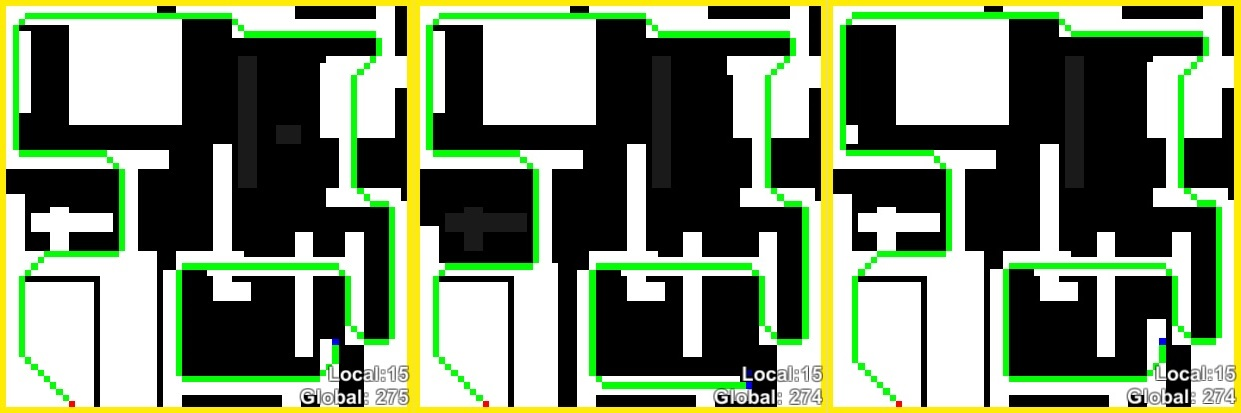
\includegraphics[width=1\textwidth]{Imagens/maps_ag.jpg}
	\end{center}
\end{figure}

\FloatBarrier
\pagebreak

\section{Busca Inovativa}

Mapas contidos no conjunto $C_f$ da 3ª execução da configuração \textbf{NS}.

\begin{figure}[htb]
	\begin{center}
		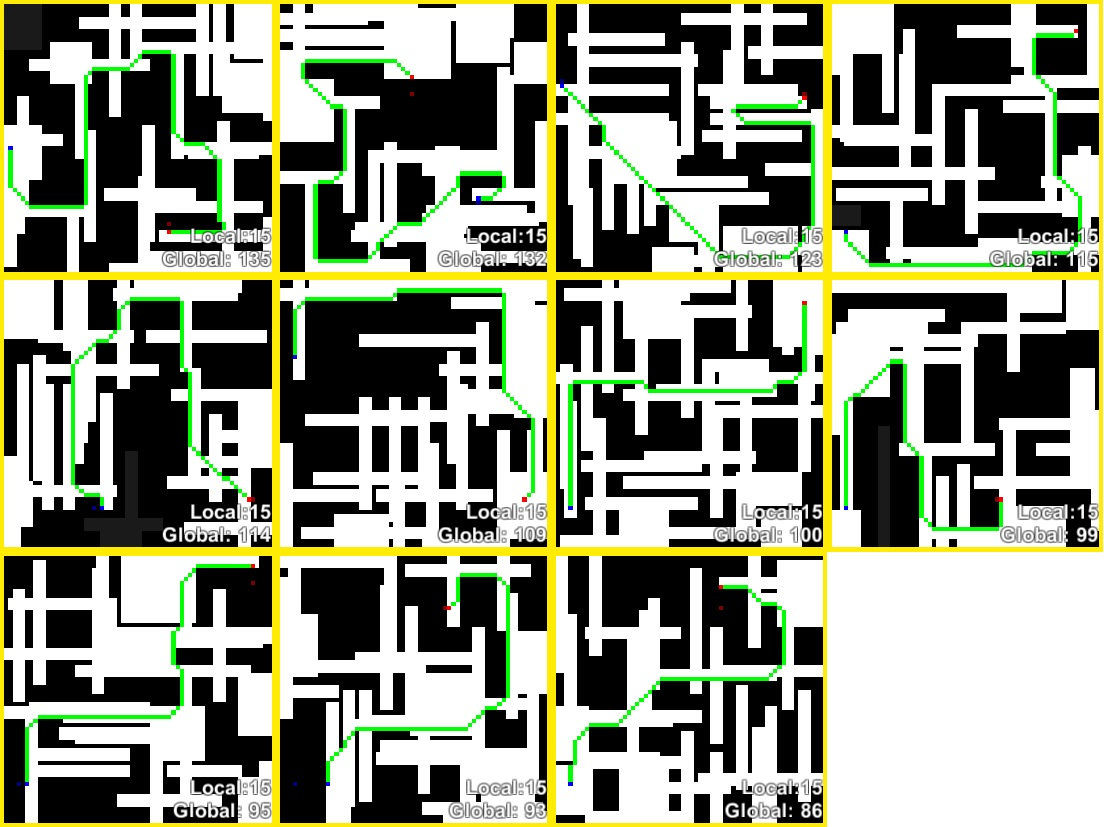
\includegraphics[width=1\textwidth]{Imagens/maps_ns.jpg}
	\end{center}
\end{figure}

\FloatBarrier
\pagebreak

\section{Competição Local}

Mapas contidos no conjunto $C_f$ da 3ª execução da configuração \textbf{Lehman}.

\begin{figure}[htb]
	\begin{center}
		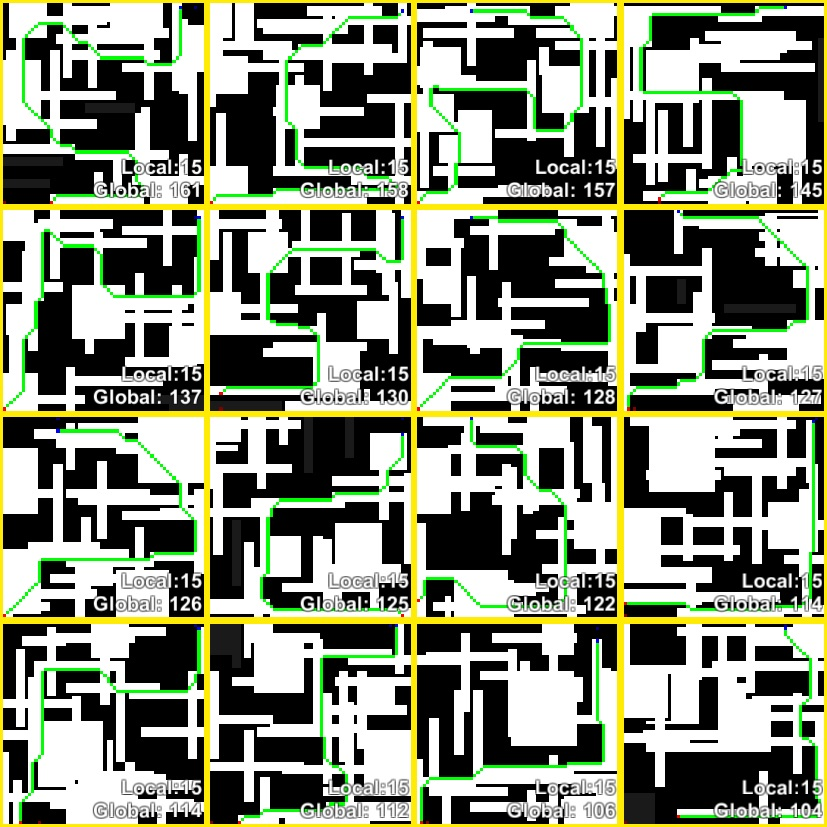
\includegraphics[width=1\textwidth]{Imagens/maps_lehman.jpg}
	\end{center}
\end{figure}

\FloatBarrier
\pagebreak

\section{Proposta}

Mapas contidos no conjunto $C_f$ da 6ª execução da configuração \textbf{Proposta}.

\begin{figure}[htb]
	\begin{center}
		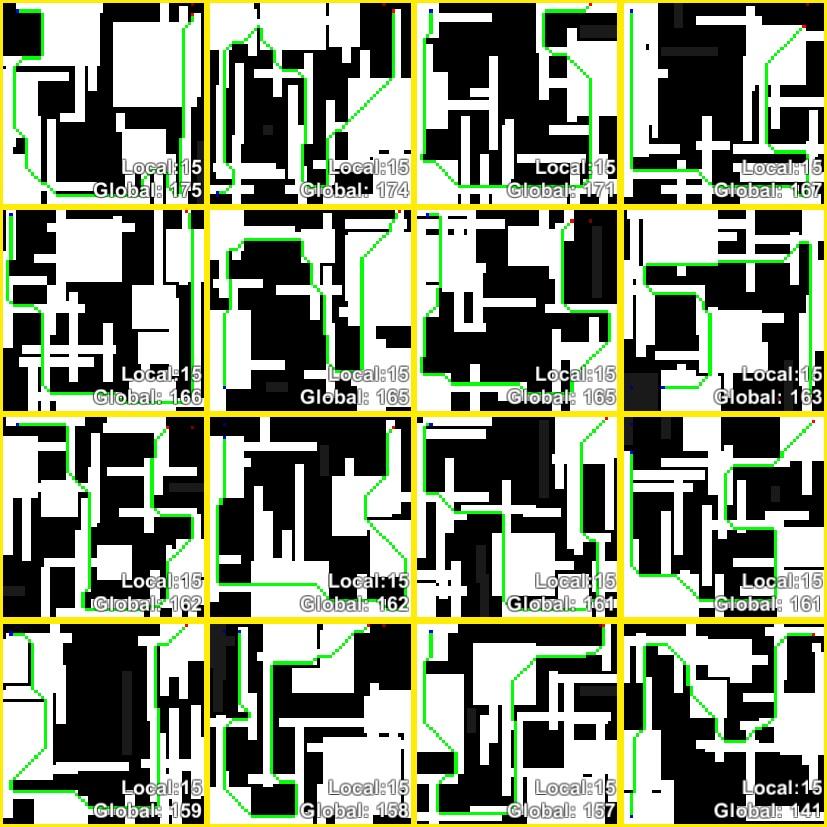
\includegraphics[width=1\textwidth]{Imagens/maps_melotti.jpg}
	\end{center}
\end{figure}

\FloatBarrier

\end{document}
% ----------------------------------------------------------------
